\documentclass[twoside]{book}

% Packages required by doxygen
\usepackage{calc}
\usepackage{doxygen}
\usepackage{graphicx}
\usepackage[utf8]{inputenc}
\usepackage{makeidx}
\usepackage{multicol}
\usepackage{multirow}
\usepackage{textcomp}
\usepackage[table]{xcolor}

% Font selection
\usepackage[T1]{fontenc}
\usepackage{mathptmx}
\usepackage[scaled=.90]{helvet}
\usepackage{courier}
\usepackage{amssymb}
\usepackage{sectsty}
\renewcommand{\familydefault}{\sfdefault}
\allsectionsfont{%
  \fontseries{bc}\selectfont%
  \color{darkgray}%
}
\renewcommand{\DoxyLabelFont}{%
  \fontseries{bc}\selectfont%
  \color{darkgray}%
}

% Page & text layout
\usepackage{geometry}
\geometry{%
  a4paper,%
  top=2.5cm,%
  bottom=2.5cm,%
  left=2.5cm,%
  right=2.5cm%
}
\tolerance=750
\hfuzz=15pt
\hbadness=750
\setlength{\emergencystretch}{15pt}
\setlength{\parindent}{0cm}
\setlength{\parskip}{0.2cm}
\makeatletter
\renewcommand{\paragraph}{%
  \@startsection{paragraph}{4}{0ex}{-1.0ex}{1.0ex}{%
    \normalfont\normalsize\bfseries\SS@parafont%
  }%
}
\renewcommand{\subparagraph}{%
  \@startsection{subparagraph}{5}{0ex}{-1.0ex}{1.0ex}{%
    \normalfont\normalsize\bfseries\SS@subparafont%
  }%
}
\makeatother

% Headers & footers
\usepackage{fancyhdr}
\pagestyle{fancyplain}
\fancyhead[LE]{\fancyplain{}{\bfseries\thepage}}
\fancyhead[CE]{\fancyplain{}{}}
\fancyhead[RE]{\fancyplain{}{\bfseries\leftmark}}
\fancyhead[LO]{\fancyplain{}{\bfseries\rightmark}}
\fancyhead[CO]{\fancyplain{}{}}
\fancyhead[RO]{\fancyplain{}{\bfseries\thepage}}
\fancyfoot[LE]{\fancyplain{}{}}
\fancyfoot[CE]{\fancyplain{}{}}
\fancyfoot[RE]{\fancyplain{}{\bfseries\scriptsize Generated on Fri Feb 21 2014 01\-:03\-:25 for Hoa\-Library by Doxygen }}
\fancyfoot[LO]{\fancyplain{}{\bfseries\scriptsize Generated on Fri Feb 21 2014 01\-:03\-:25 for Hoa\-Library by Doxygen }}
\fancyfoot[CO]{\fancyplain{}{}}
\fancyfoot[RO]{\fancyplain{}{}}
\renewcommand{\footrulewidth}{0.4pt}
\renewcommand{\chaptermark}[1]{%
  \markboth{#1}{}%
}
\renewcommand{\sectionmark}[1]{%
  \markright{\thesection\ #1}%
}

% Indices & bibliography
\usepackage{natbib}
\usepackage[titles]{tocloft}
\setcounter{tocdepth}{3}
\setcounter{secnumdepth}{5}
\makeindex

% Hyperlinks (required, but should be loaded last)
\usepackage{ifpdf}
\ifpdf
  \usepackage[pdftex,pagebackref=true]{hyperref}
\else
  \usepackage[ps2pdf,pagebackref=true]{hyperref}
\fi
\hypersetup{%
  colorlinks=true,%
  linkcolor=blue,%
  citecolor=blue,%
  unicode%
}

% Custom commands
\newcommand{\clearemptydoublepage}{%
  \newpage{\pagestyle{empty}\cleardoublepage}%
}


%===== C O N T E N T S =====

\begin{document}

% Titlepage & ToC
\hypersetup{pageanchor=false}
\pagenumbering{roman}
\begin{titlepage}
\vspace*{7cm}
\begin{center}%
{\Large Hoa\-Library \\[1ex]\large 2.\-0 }\\
\vspace*{1cm}
{\large Generated by Doxygen 1.8.5}\\
\vspace*{0.5cm}
{\small Fri Feb 21 2014 01:03:25}\\
\end{center}
\end{titlepage}
\clearemptydoublepage
\tableofcontents
\clearemptydoublepage
\pagenumbering{arabic}
\hypersetup{pageanchor=true}

%--- Begin generated contents ---
\chapter{Namespace Index}
\section{Namespace List}
Here is a list of all documented namespaces with brief descriptions\-:\begin{DoxyCompactList}
\item\contentsline{section}{\hyperlink{namespace_hoa}{Hoa} \\*The high order ambisonic namespace }{\pageref{namespace_hoa}}{}
\item\contentsline{section}{\hyperlink{namespace_hoa2_d}{Hoa2\-D} \\*The 2\-D high order ambisonic namespace }{\pageref{namespace_hoa2_d}}{}
\item\contentsline{section}{\hyperlink{namespace_hoa3_d}{Hoa3\-D} \\*The 3\-D ambisonic classes }{\pageref{namespace_hoa3_d}}{}
\end{DoxyCompactList}

\chapter{Hierarchical Index}
\section{Class Hierarchy}
This inheritance list is sorted roughly, but not completely, alphabetically\-:\begin{DoxyCompactList}
\item \contentsline{section}{Hoa\-:\-:\-\_\-hoa\-\_\-rgb}{\pageref{struct_hoa_1_1__hoa__rgb}}{}
\item \contentsline{section}{Hoa\-:\-:\-\_\-hoa\-\_\-rgba}{\pageref{struct_hoa_1_1__hoa__rgba}}{}
\item \contentsline{section}{Hoa2\-D\-:\-:Ambisonic}{\pageref{class_hoa2_d_1_1_ambisonic}}{}
\begin{DoxyCompactList}
\item \contentsline{section}{Hoa2\-D\-:\-:Decoder\-Binaural}{\pageref{class_hoa2_d_1_1_decoder_binaural}}{}
\item \contentsline{section}{Hoa2\-D\-:\-:Decoder\-Irregular}{\pageref{class_hoa2_d_1_1_decoder_irregular}}{}
\item \contentsline{section}{Hoa2\-D\-:\-:Decoder\-Regular}{\pageref{class_hoa2_d_1_1_decoder_regular}}{}
\item \contentsline{section}{Hoa2\-D\-:\-:Encoder}{\pageref{class_hoa2_d_1_1_encoder}}{}
\item \contentsline{section}{Hoa2\-D\-:\-:Map}{\pageref{class_hoa2_d_1_1_map}}{}
\item \contentsline{section}{Hoa2\-D\-:\-:Optim}{\pageref{class_hoa2_d_1_1_optim}}{}
\item \contentsline{section}{Hoa2\-D\-:\-:Projector}{\pageref{class_hoa2_d_1_1_projector}}{}
\item \contentsline{section}{Hoa2\-D\-:\-:Recomposer}{\pageref{class_hoa2_d_1_1_recomposer}}{}
\item \contentsline{section}{Hoa2\-D\-:\-:Rotate}{\pageref{class_hoa2_d_1_1_rotate}}{}
\item \contentsline{section}{Hoa2\-D\-:\-:Scope}{\pageref{class_hoa2_d_1_1_scope}}{}
\item \contentsline{section}{Hoa2\-D\-:\-:Wider}{\pageref{class_hoa2_d_1_1_wider}}{}
\end{DoxyCompactList}
\item \contentsline{section}{Hoa3\-D\-:\-:Ambisonic}{\pageref{class_hoa3_d_1_1_ambisonic}}{}
\begin{DoxyCompactList}
\item \contentsline{section}{Hoa3\-D\-:\-:Decoder}{\pageref{class_hoa3_d_1_1_decoder}}{}
\item \contentsline{section}{Hoa3\-D\-:\-:Encoder}{\pageref{class_hoa3_d_1_1_encoder}}{}
\item \contentsline{section}{Hoa3\-D\-:\-:Map}{\pageref{class_hoa3_d_1_1_map}}{}
\item \contentsline{section}{Hoa3\-D\-:\-:Optim}{\pageref{class_hoa3_d_1_1_optim}}{}
\item \contentsline{section}{Hoa3\-D\-:\-:Rotate}{\pageref{class_hoa3_d_1_1_rotate}}{}
\item \contentsline{section}{Hoa3\-D\-:\-:Scope}{\pageref{class_hoa3_d_1_1_scope}}{}
\item \contentsline{section}{Hoa3\-D\-:\-:Wider}{\pageref{class_hoa3_d_1_1_wider}}{}
\end{DoxyCompactList}
\item \contentsline{section}{Ambisonic\-Virtual\-Mic\-U\-I}{\pageref{class_ambisonic_virtual_mic_u_i}}{}
\item \contentsline{section}{Ambisonic\-Virtual\-Mic\-U\-I\-Manager}{\pageref{class_ambisonic_virtual_mic_u_i_manager}}{}
\item \contentsline{section}{Hoa\-:\-:coordinates\-Cartesian}{\pageref{struct_hoa_1_1coordinates_cartesian}}{}
\item \contentsline{section}{Hoa\-:\-:coordinates\-Polar}{\pageref{struct_hoa_1_1coordinates_polar}}{}
\item \contentsline{section}{Hoa3\-D\-:\-:Planewaves}{\pageref{class_hoa3_d_1_1_planewaves}}{}
\begin{DoxyCompactList}
\item \contentsline{section}{Hoa3\-D\-:\-:Meter}{\pageref{class_hoa3_d_1_1_meter}}{}
\item \contentsline{section}{Hoa3\-D\-:\-:Vector}{\pageref{class_hoa3_d_1_1_vector}}{}
\end{DoxyCompactList}
\item Planewaves\begin{DoxyCompactList}
\item \contentsline{section}{Ambisonics\-Meter}{\pageref{class_ambisonics_meter}}{}
\end{DoxyCompactList}
\item \contentsline{section}{Hoa2\-D\-:\-:Planewaves}{\pageref{class_hoa2_d_1_1_planewaves}}{}
\begin{DoxyCompactList}
\item \contentsline{section}{Hoa2\-D\-:\-:Decoder\-Binaural}{\pageref{class_hoa2_d_1_1_decoder_binaural}}{}
\item \contentsline{section}{Hoa2\-D\-:\-:Decoder\-Irregular}{\pageref{class_hoa2_d_1_1_decoder_irregular}}{}
\item \contentsline{section}{Hoa2\-D\-:\-:Decoder\-Regular}{\pageref{class_hoa2_d_1_1_decoder_regular}}{}
\item \contentsline{section}{Hoa2\-D\-:\-:Meter}{\pageref{class_hoa2_d_1_1_meter}}{}
\item \contentsline{section}{Hoa2\-D\-:\-:Projector}{\pageref{class_hoa2_d_1_1_projector}}{}
\item \contentsline{section}{Hoa2\-D\-:\-:Recomposer}{\pageref{class_hoa2_d_1_1_recomposer}}{}
\item \contentsline{section}{Hoa2\-D\-:\-:Vector}{\pageref{class_hoa2_d_1_1_vector}}{}
\end{DoxyCompactList}
\item \contentsline{section}{Hoa2\-D\-:\-:Source}{\pageref{class_hoa2_d_1_1_source}}{}
\item \contentsline{section}{Hoa2\-D\-:\-:Sources\-Group}{\pageref{class_hoa2_d_1_1_sources_group}}{}
\item \contentsline{section}{Hoa2\-D\-:\-:Sources\-Manager}{\pageref{class_hoa2_d_1_1_sources_manager}}{}
\item \contentsline{section}{Hoa2\-D\-:\-:Sources\-Preset}{\pageref{class_hoa2_d_1_1_sources_preset}}{}
\begin{DoxyCompactList}
\item \contentsline{section}{Hoa2\-D\-:\-:Sources\-Trajectory}{\pageref{class_hoa2_d_1_1_sources_trajectory}}{}
\end{DoxyCompactList}
\item \contentsline{section}{Tools}{\pageref{class_tools}}{}
\end{DoxyCompactList}

\chapter{Class Index}
\section{Class List}
Here are the classes, structs, unions and interfaces with brief descriptions\-:\begin{DoxyCompactList}
\item\contentsline{section}{\hyperlink{class_hoa2_d_1_1_ambisonic}{Hoa2\-D\-::\-Ambisonic} \\*The ambisonic class }{\pageref{class_hoa2_d_1_1_ambisonic}}{}
\item\contentsline{section}{\hyperlink{class_hoa3_d_1_1_ambisonic}{Hoa3\-D\-::\-Ambisonic} \\*The ambisonic class }{\pageref{class_hoa3_d_1_1_ambisonic}}{}
\item\contentsline{section}{\hyperlink{class_ambisonic}{Ambisonic} }{\pageref{class_ambisonic}}{}
\item\contentsline{section}{\hyperlink{class_ambisonic_convolver}{Ambisonic\-Convolver} }{\pageref{class_ambisonic_convolver}}{}
\item\contentsline{section}{\hyperlink{class_ambisonic_encoder}{Ambisonic\-Encoder} \\*An ambisonic encoder }{\pageref{class_ambisonic_encoder}}{}
\item\contentsline{section}{\hyperlink{class_ambisonic_freeverb}{Ambisonic\-Freeverb} }{\pageref{class_ambisonic_freeverb}}{}
\item\contentsline{section}{\hyperlink{class_ambisonic_map}{Ambisonic\-Map} }{\pageref{class_ambisonic_map}}{}
\item\contentsline{section}{\hyperlink{class_ambisonic_one_pole}{Ambisonic\-One\-Pole} }{\pageref{class_ambisonic_one_pole}}{}
\item\contentsline{section}{\hyperlink{class_ambisonic_optim}{Ambisonic\-Optim} }{\pageref{class_ambisonic_optim}}{}
\item\contentsline{section}{\hyperlink{class_ambisonic_projector}{Ambisonic\-Projector} }{\pageref{class_ambisonic_projector}}{}
\item\contentsline{section}{\hyperlink{class_ambisonic_recomposer}{Ambisonic\-Recomposer} }{\pageref{class_ambisonic_recomposer}}{}
\item\contentsline{section}{\hyperlink{class_ambisonic_rotate}{Ambisonic\-Rotate} }{\pageref{class_ambisonic_rotate}}{}
\item\contentsline{section}{\hyperlink{class_ambisonics_binaural}{Ambisonics\-Binaural} }{\pageref{class_ambisonics_binaural}}{}
\item\contentsline{section}{\hyperlink{class_ambisonics_decoder}{Ambisonics\-Decoder} }{\pageref{class_ambisonics_decoder}}{}
\item\contentsline{section}{\hyperlink{class_ambisonics_delay}{Ambisonics\-Delay} }{\pageref{class_ambisonics_delay}}{}
\item\contentsline{section}{\hyperlink{class_ambisonics_diffuser}{Ambisonics\-Diffuser} }{\pageref{class_ambisonics_diffuser}}{}
\item\contentsline{section}{\hyperlink{class_ambisonics_filter}{Ambisonics\-Filter} }{\pageref{class_ambisonics_filter}}{}
\item\contentsline{section}{\hyperlink{class_ambisonics_freeverb}{Ambisonics\-Freeverb} }{\pageref{class_ambisonics_freeverb}}{}
\item\contentsline{section}{\hyperlink{class_ambisonics_grain}{Ambisonics\-Grain} }{\pageref{class_ambisonics_grain}}{}
\item\contentsline{section}{\hyperlink{class_ambisonics_meter}{Ambisonics\-Meter} }{\pageref{class_ambisonics_meter}}{}
\item\contentsline{section}{\hyperlink{class_ambisonics_multi_decoder}{Ambisonics\-Multi\-Decoder} }{\pageref{class_ambisonics_multi_decoder}}{}
\item\contentsline{section}{\hyperlink{class_ambisonics_multi_maps}{Ambisonics\-Multi\-Maps} }{\pageref{class_ambisonics_multi_maps}}{}
\item\contentsline{section}{\hyperlink{class_ambisonic_space}{Ambisonic\-Space} }{\pageref{class_ambisonic_space}}{}
\item\contentsline{section}{\hyperlink{class_ambisonic_spectrum}{Ambisonic\-Spectrum} }{\pageref{class_ambisonic_spectrum}}{}
\item\contentsline{section}{\hyperlink{class_ambisonics_restitution}{Ambisonics\-Restitution} }{\pageref{class_ambisonics_restitution}}{}
\item\contentsline{section}{\hyperlink{class_ambisonics_ring_modulation}{Ambisonics\-Ring\-Modulation} }{\pageref{class_ambisonics_ring_modulation}}{}
\item\contentsline{section}{\hyperlink{class_ambisonics_scope}{Ambisonics\-Scope} }{\pageref{class_ambisonics_scope}}{}
\item\contentsline{section}{\hyperlink{class_ambisonic_vector}{Ambisonic\-Vector} }{\pageref{class_ambisonic_vector}}{}
\item\contentsline{section}{\hyperlink{class_ambisonic_viewer}{Ambisonic\-Viewer} }{\pageref{class_ambisonic_viewer}}{}
\item\contentsline{section}{\hyperlink{class_ambisonic_virtual_mic_u_i}{Ambisonic\-Virtual\-Mic\-U\-I} }{\pageref{class_ambisonic_virtual_mic_u_i}}{}
\item\contentsline{section}{\hyperlink{class_ambisonic_virtual_mic_u_i_manager}{Ambisonic\-Virtual\-Mic\-U\-I\-Manager} }{\pageref{class_ambisonic_virtual_mic_u_i_manager}}{}
\item\contentsline{section}{\hyperlink{class_ambisonic_wider}{Ambisonic\-Wider} \\*An ambisonic wider }{\pageref{class_ambisonic_wider}}{}
\item\contentsline{section}{\hyperlink{class_boid}{Boid} }{\pageref{class_boid}}{}
\item\contentsline{section}{\hyperlink{class_boids_manager}{Boids\-Manager} }{\pageref{class_boids_manager}}{}
\item\contentsline{section}{\hyperlink{struct_box2_d}{Box2\-D} }{\pageref{struct_box2_d}}{}
\item\contentsline{section}{\hyperlink{class_cicm___fft}{Cicm\-\_\-\-Fft} }{\pageref{class_cicm___fft}}{}
\item\contentsline{section}{\hyperlink{class_cicm_decorrelation}{Cicm\-Decorrelation} }{\pageref{class_cicm_decorrelation}}{}
\item\contentsline{section}{\hyperlink{class_cicm_envelope}{Cicm\-Envelope} }{\pageref{class_cicm_envelope}}{}
\item\contentsline{section}{\hyperlink{class_cicm_filter_delay}{Cicm\-Filter\-Delay} }{\pageref{class_cicm_filter_delay}}{}
\item\contentsline{section}{\hyperlink{class_cicm_line}{Cicm\-Line} }{\pageref{class_cicm_line}}{}
\item\contentsline{section}{\hyperlink{class_cicm_qsgs}{Cicm\-Qsgs} }{\pageref{class_cicm_qsgs}}{}
\item\contentsline{section}{\hyperlink{class_cicm_ring_modulation}{Cicm\-Ring\-Modulation} }{\pageref{class_cicm_ring_modulation}}{}
\item\contentsline{section}{\hyperlink{structcolor}{color} }{\pageref{structcolor}}{}
\item\contentsline{section}{\hyperlink{structcoordinates_cartesian}{coordinates\-Cartesian} }{\pageref{structcoordinates_cartesian}}{}
\item\contentsline{section}{\hyperlink{structcoordinates_polar}{coordinates\-Polar} }{\pageref{structcoordinates_polar}}{}
\item\contentsline{section}{\hyperlink{class_hoa3_d_1_1_decoder}{Hoa3\-D\-::\-Decoder} \\*The ambisonic decoder }{\pageref{class_hoa3_d_1_1_decoder}}{}
\item\contentsline{section}{\hyperlink{class_hoa2_d_1_1_decoder}{Hoa2\-D\-::\-Decoder} }{\pageref{class_hoa2_d_1_1_decoder}}{}
\item\contentsline{section}{\hyperlink{class_hoa3_d_1_1_encoder}{Hoa3\-D\-::\-Encoder} \\*The ambisonic encoder }{\pageref{class_hoa3_d_1_1_encoder}}{}
\item\contentsline{section}{\hyperlink{class_hoa2_d_1_1_encoder}{Hoa2\-D\-::\-Encoder} \\*The ambisonic encoder }{\pageref{class_hoa2_d_1_1_encoder}}{}
\item\contentsline{section}{\hyperlink{class_filter}{Filter} }{\pageref{class_filter}}{}
\item\contentsline{section}{\hyperlink{class_filter_allpass}{Filter\-Allpass} }{\pageref{class_filter_allpass}}{}
\item\contentsline{section}{\hyperlink{class_filter_biquad}{Filter\-Biquad} }{\pageref{class_filter_biquad}}{}
\item\contentsline{section}{\hyperlink{class_filter_comb}{Filter\-Comb} }{\pageref{class_filter_comb}}{}
\item\contentsline{section}{\hyperlink{class_filter_convolution}{Filter\-Convolution} }{\pageref{class_filter_convolution}}{}
\item\contentsline{section}{\hyperlink{class_filter_convolution_zero}{Filter\-Convolution\-Zero} }{\pageref{class_filter_convolution_zero}}{}
\item\contentsline{section}{\hyperlink{class_filter_damper}{Filter\-Damper} }{\pageref{class_filter_damper}}{}
\item\contentsline{section}{\hyperlink{class_filter_diffuser}{Filter\-Diffuser} }{\pageref{class_filter_diffuser}}{}
\item\contentsline{section}{\hyperlink{class_filter_fir}{Filter\-Fir} }{\pageref{class_filter_fir}}{}
\item\contentsline{section}{\hyperlink{class_filter_fixed_delay}{Filter\-Fixed\-Delay} }{\pageref{class_filter_fixed_delay}}{}
\item\contentsline{section}{\hyperlink{class_filter_one_pole}{Filter\-One\-Pole} }{\pageref{class_filter_one_pole}}{}
\item\contentsline{section}{\hyperlink{class_freeverb}{Freeverb} }{\pageref{class_freeverb}}{}
\item\contentsline{section}{\hyperlink{class_hoa3_d_1_1_map}{Hoa3\-D\-::\-Map} \\*The ambisonic map }{\pageref{class_hoa3_d_1_1_map}}{}
\item\contentsline{section}{\hyperlink{class_hoa3_d_1_1_meter}{Hoa3\-D\-::\-Meter} \\*The ambisonic \hyperlink{class_hoa3_d_1_1_meter}{Meter} }{\pageref{class_hoa3_d_1_1_meter}}{}
\item\contentsline{section}{\hyperlink{class_hoa2_d_1_1_optim}{Hoa2\-D\-::\-Optim} \\*The ambisonic optimization }{\pageref{class_hoa2_d_1_1_optim}}{}
\item\contentsline{section}{\hyperlink{class_hoa3_d_1_1_optim}{Hoa3\-D\-::\-Optim} \\*The ambisonic optimization }{\pageref{class_hoa3_d_1_1_optim}}{}
\item\contentsline{section}{\hyperlink{class_hoa3_d_1_1_planewaves}{Hoa3\-D\-::\-Planewaves} \\*The planewaves class }{\pageref{class_hoa3_d_1_1_planewaves}}{}
\item\contentsline{section}{\hyperlink{class_planewaves}{Planewaves} }{\pageref{class_planewaves}}{}
\item\contentsline{section}{\hyperlink{struct_point2d}{Point2d} }{\pageref{struct_point2d}}{}
\item\contentsline{section}{\hyperlink{class_hoa2_d_1_1_rotate}{Hoa2\-D\-::\-Rotate} \\*The ambisonic rotation }{\pageref{class_hoa2_d_1_1_rotate}}{}
\item\contentsline{section}{\hyperlink{class_hoa3_d_1_1_rotate}{Hoa3\-D\-::\-Rotate} \\*The ambisonic rotate }{\pageref{class_hoa3_d_1_1_rotate}}{}
\item\contentsline{section}{\hyperlink{class_hoa3_d_1_1_scope}{Hoa3\-D\-::\-Scope} \\*The ambisonic scope }{\pageref{class_hoa3_d_1_1_scope}}{}
\item\contentsline{section}{\hyperlink{class_cicm_1_1_signal_vector_float}{Cicm\-::\-Signal\-Vector\-Float} }{\pageref{class_cicm_1_1_signal_vector_float}}{}
\item\contentsline{section}{\hyperlink{class_sources_manager}{Sources\-Manager} }{\pageref{class_sources_manager}}{}
\item\contentsline{section}{\hyperlink{class_sources_preset}{Sources\-Preset} }{\pageref{class_sources_preset}}{}
\item\contentsline{section}{\hyperlink{class_sources_trajectory}{Sources\-Trajectory} }{\pageref{class_sources_trajectory}}{}
\item\contentsline{section}{\hyperlink{class_tools}{Tools} }{\pageref{class_tools}}{}
\item\contentsline{section}{\hyperlink{class_hoa3_d_1_1_vector}{Hoa3\-D\-::\-Vector} \\*The ambisonic vector }{\pageref{class_hoa3_d_1_1_vector}}{}
\item\contentsline{section}{\hyperlink{struct_velocity}{Velocity} }{\pageref{struct_velocity}}{}
\item\contentsline{section}{\hyperlink{class_hoa3_d_1_1_wider}{Hoa3\-D\-::\-Wider} \\*The ambisonic wider }{\pageref{class_hoa3_d_1_1_wider}}{}
\end{DoxyCompactList}

\chapter{Namespace Documentation}
\hypertarget{namespace_hoa2_d}{\section{Hoa2\-D Namespace Reference}
\label{namespace_hoa2_d}\index{Hoa2\-D@{Hoa2\-D}}
}


The 2\-D high order ambisonic namespace.  


\subsection*{Classes}
\begin{DoxyCompactItemize}
\item 
class \hyperlink{class_hoa2_d_1_1_ambisonic}{Ambisonic}
\begin{DoxyCompactList}\small\item\em The ambisonic class. \end{DoxyCompactList}\item 
class \hyperlink{class_hoa2_d_1_1_channel_manager}{Channel\-Manager}
\begin{DoxyCompactList}\small\item\em The channel manager. \end{DoxyCompactList}\item 
class \hyperlink{class_hoa2_d_1_1_decoder_regular}{Decoder\-Regular}
\begin{DoxyCompactList}\small\item\em The ambisonic regular decoder. \end{DoxyCompactList}\item 
class \hyperlink{class_hoa2_d_1_1_decoder_irregular}{Decoder\-Irregular}
\begin{DoxyCompactList}\small\item\em The ambisonic irregular decoder. \end{DoxyCompactList}\item 
class \hyperlink{class_hoa2_d_1_1_decoder_binaural}{Decoder\-Binaural}
\begin{DoxyCompactList}\small\item\em The ambisonic binaural decoder. \end{DoxyCompactList}\item 
class \hyperlink{class_hoa2_d_1_1_decoder_multi}{Decoder\-Multi}
\begin{DoxyCompactList}\small\item\em The ambisonic multi-\/decoder. \end{DoxyCompactList}\item 
class \hyperlink{class_hoa2_d_1_1_encoder}{Encoder}
\begin{DoxyCompactList}\small\item\em The ambisonic encoder. \end{DoxyCompactList}\item 
class \hyperlink{class_hoa2_d_1_1_kit_sources}{Kit\-Sources}
\begin{DoxyCompactList}\small\item\em The kit to spatialize lught points sources. \end{DoxyCompactList}\item 
class \hyperlink{class_hoa2_d_1_1_map}{Map}
\begin{DoxyCompactList}\small\item\em The ambisonic multi-\/encoder with distance compensation. \end{DoxyCompactList}\item 
class \hyperlink{class_hoa2_d_1_1_meter}{Meter}
\begin{DoxyCompactList}\small\item\em The planewaves peak level meter. \end{DoxyCompactList}\item 
class \hyperlink{class_hoa2_d_1_1_optim}{Optim}
\begin{DoxyCompactList}\small\item\em The ambisonic optimization. \end{DoxyCompactList}\item 
class \hyperlink{class_hoa2_d_1_1_planewaves}{Planewaves}
\begin{DoxyCompactList}\small\item\em The planewaves class. \end{DoxyCompactList}\item 
class \hyperlink{class_hoa2_d_1_1_projector}{Projector}
\begin{DoxyCompactList}\small\item\em The ambisonic projector. \end{DoxyCompactList}\item 
class \hyperlink{class_hoa2_d_1_1_recomposer}{Recomposer}
\begin{DoxyCompactList}\small\item\em The ambisonic recomposer. \end{DoxyCompactList}\item 
class \hyperlink{class_hoa2_d_1_1_rotate}{Rotate}
\begin{DoxyCompactList}\small\item\em The ambisonic rotation. \end{DoxyCompactList}\item 
class \hyperlink{class_hoa2_d_1_1_scope}{Scope}
\begin{DoxyCompactList}\small\item\em The ambisonic scope. \end{DoxyCompactList}\item 
class \hyperlink{class_hoa2_d_1_1_source}{Source}
\begin{DoxyCompactList}\small\item\em The source. \end{DoxyCompactList}\item 
class \hyperlink{class_hoa2_d_1_1_sources_group}{Sources\-Group}
\begin{DoxyCompactList}\small\item\em The sources group. \end{DoxyCompactList}\item 
class \hyperlink{class_hoa2_d_1_1_sources_manager}{Sources\-Manager}
\begin{DoxyCompactList}\small\item\em The sources manager. \end{DoxyCompactList}\item 
class \hyperlink{class_hoa2_d_1_1_sources_preset}{Sources\-Preset}
\begin{DoxyCompactList}\small\item\em The sources preset. \end{DoxyCompactList}\item 
class \hyperlink{class_hoa2_d_1_1_sources_trajectory}{Sources\-Trajectory}
\begin{DoxyCompactList}\small\item\em The sources trajectory. \end{DoxyCompactList}\item 
class \hyperlink{class_hoa2_d_1_1_vector}{Vector}
\begin{DoxyCompactList}\small\item\em The ambisonic vector. \end{DoxyCompactList}\item 
class \hyperlink{class_hoa2_d_1_1_wider}{Wider}
\begin{DoxyCompactList}\small\item\em The ambisonic wider. \end{DoxyCompactList}\end{DoxyCompactItemize}


\subsection{Detailed Description}
The 2\-D high order ambisonic namespace. All the 2\-D ambisonic classes will be part of this namespace 
\hypertarget{namespace_hoa3_d}{\section{Hoa3\-D Namespace Reference}
\label{namespace_hoa3_d}\index{Hoa3\-D@{Hoa3\-D}}
}


The 3\-D ambisonic classes.  


\subsection*{Classes}
\begin{DoxyCompactItemize}
\item 
class \hyperlink{class_hoa3_d_1_1_ambisonic}{Ambisonic}
\begin{DoxyCompactList}\small\item\em The ambisonic class. \end{DoxyCompactList}\item 
class \hyperlink{class_hoa3_d_1_1_decoder}{Decoder}
\begin{DoxyCompactList}\small\item\em The ambisonic decoder. \end{DoxyCompactList}\item 
class \hyperlink{class_hoa3_d_1_1_encoder}{Encoder}
\begin{DoxyCompactList}\small\item\em The ambisonic encoder. \end{DoxyCompactList}\item 
class \hyperlink{class_hoa3_d_1_1_map}{Map}
\begin{DoxyCompactList}\small\item\em The ambisonic map. \end{DoxyCompactList}\item 
class \hyperlink{class_hoa3_d_1_1_meter}{Meter}
\begin{DoxyCompactList}\small\item\em The ambisonic \hyperlink{class_hoa3_d_1_1_meter}{Meter}. \end{DoxyCompactList}\item 
class \hyperlink{class_hoa3_d_1_1_optim}{Optim}
\begin{DoxyCompactList}\small\item\em The ambisonic optimization. \end{DoxyCompactList}\item 
class \hyperlink{class_hoa3_d_1_1_planewaves}{Planewaves}
\begin{DoxyCompactList}\small\item\em The planewaves class. \end{DoxyCompactList}\item 
class \hyperlink{class_hoa3_d_1_1_rotate}{Rotate}
\begin{DoxyCompactList}\small\item\em The ambisonic rotate. \end{DoxyCompactList}\item 
class \hyperlink{class_hoa3_d_1_1_scope}{Scope}
\begin{DoxyCompactList}\small\item\em The ambisonic scope. \end{DoxyCompactList}\item 
class \hyperlink{class_hoa3_d_1_1_vector}{Vector}
\begin{DoxyCompactList}\small\item\em The ambisonic vector. \end{DoxyCompactList}\item 
class \hyperlink{class_hoa3_d_1_1_wider}{Wider}
\begin{DoxyCompactList}\small\item\em The ambisonic wider. \end{DoxyCompactList}\end{DoxyCompactItemize}


\subsection{Detailed Description}
The 3\-D ambisonic classes. All the 3\-D ambisonic and planewaves classes will be part of this namespace 
\chapter{Class Documentation}
\hypertarget{class_hoa2_d_1_1_ambisonic}{\section{Hoa2\-D\-:\-:Ambisonic Class Reference}
\label{class_hoa2_d_1_1_ambisonic}\index{Hoa2\-D\-::\-Ambisonic@{Hoa2\-D\-::\-Ambisonic}}
}


The ambisonic class.  




{\ttfamily \#include $<$Ambisonic.\-h$>$}

Inheritance diagram for Hoa2\-D\-:\-:Ambisonic\-:\begin{figure}[H]
\begin{center}
\leavevmode
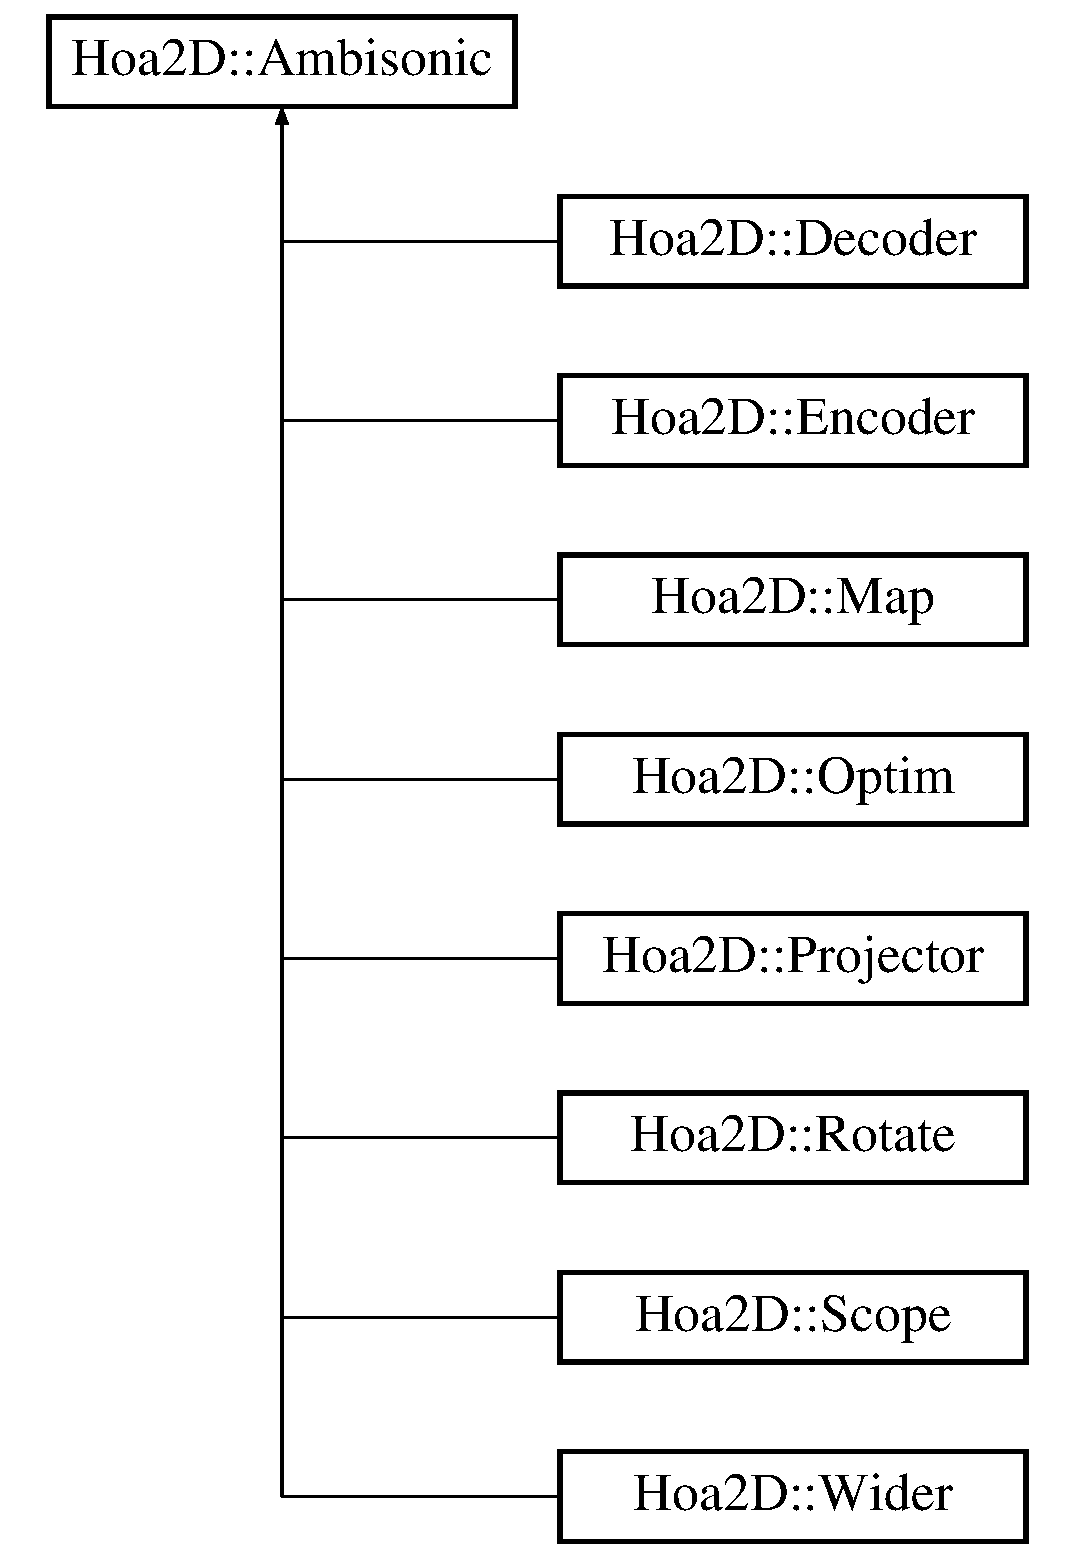
\includegraphics[height=12.000000cm]{class_hoa2_d_1_1_ambisonic}
\end{center}
\end{figure}
\subsection*{Public Member Functions}
\begin{DoxyCompactItemize}
\item 
\hyperlink{class_hoa2_d_1_1_ambisonic_ac53cc3ea0b6600dd84d761f89b5af9d3}{Ambisonic} (unsigned int order)
\begin{DoxyCompactList}\small\item\em The ambisonic constructor. \end{DoxyCompactList}\item 
\hyperlink{class_hoa2_d_1_1_ambisonic_a27be996cfb2bad88e13a32c0d7dba517}{$\sim$\-Ambisonic} ()
\item 
unsigned int \hyperlink{class_hoa2_d_1_1_ambisonic_a00797f96b864e2913567e08239ed9593}{get\-Order} () const 
\item 
unsigned int \hyperlink{class_hoa2_d_1_1_ambisonic_ae7cee18218c9bf00091d83e661d487ee}{get\-Number\-Of\-Harmonics} () const 
\item 
long \hyperlink{class_hoa2_d_1_1_ambisonic_a68c389087fb999101a499f6849b635f9}{get\-Harmonic\-Argument} (unsigned int index) const 
\begin{DoxyCompactList}\small\item\em Retrieve the argument of an harmonic. \end{DoxyCompactList}\item 
long \hyperlink{class_hoa2_d_1_1_ambisonic_a9485abf2b4f1b1aec8d0da9b12cf42ed}{get\-Harmonic\-Band} (unsigned int index) const 
\begin{DoxyCompactList}\small\item\em Retrieve the band of an harmonic. \end{DoxyCompactList}\item 
std\-::string \hyperlink{class_hoa2_d_1_1_ambisonic_a6b6f6ff74792f00bf5095dc9cfec28a4}{get\-Harmonics\-Name} (unsigned int index) const 
\begin{DoxyCompactList}\small\item\em Retrieve a name for an harmonic. \end{DoxyCompactList}\end{DoxyCompactItemize}


\subsection{Detailed Description}
The ambisonic class. 

Most of the ambisonic classes inherit from this classe. It computes the number of harmonics, their arguments and their orders depending of the decomposition order. etc... 

Definition at line 18 of file Ambisonic.\-h.



\subsection{Constructor \& Destructor Documentation}
\hypertarget{class_hoa2_d_1_1_ambisonic_ac53cc3ea0b6600dd84d761f89b5af9d3}{\index{Hoa2\-D\-::\-Ambisonic@{Hoa2\-D\-::\-Ambisonic}!Ambisonic@{Ambisonic}}
\index{Ambisonic@{Ambisonic}!Hoa2D::Ambisonic@{Hoa2\-D\-::\-Ambisonic}}
\subsubsection[{Ambisonic}]{\setlength{\rightskip}{0pt plus 5cm}Hoa2\-D\-::\-Ambisonic\-::\-Ambisonic (
\begin{DoxyParamCaption}
\item[{unsigned int}]{order}
\end{DoxyParamCaption}
)}}\label{class_hoa2_d_1_1_ambisonic_ac53cc3ea0b6600dd84d761f89b5af9d3}


The ambisonic constructor. 

The ambisonic constructor allocates and initializes the generale member values depending of a decomposition order. 
\begin{DoxyParams}{Parameters}
{\em order} & The order, must be at least 1. \\
\hline
\end{DoxyParams}


Definition at line 11 of file Ambisonic.\-cpp.

\hypertarget{class_hoa2_d_1_1_ambisonic_a27be996cfb2bad88e13a32c0d7dba517}{\index{Hoa2\-D\-::\-Ambisonic@{Hoa2\-D\-::\-Ambisonic}!$\sim$\-Ambisonic@{$\sim$\-Ambisonic}}
\index{$\sim$\-Ambisonic@{$\sim$\-Ambisonic}!Hoa2D::Ambisonic@{Hoa2\-D\-::\-Ambisonic}}
\subsubsection[{$\sim$\-Ambisonic}]{\setlength{\rightskip}{0pt plus 5cm}Hoa2\-D\-::\-Ambisonic\-::$\sim$\-Ambisonic (
\begin{DoxyParamCaption}
{}
\end{DoxyParamCaption}
)}}\label{class_hoa2_d_1_1_ambisonic_a27be996cfb2bad88e13a32c0d7dba517}
The ambisonic destructor. 

Definition at line 25 of file Ambisonic.\-cpp.



\subsection{Member Function Documentation}
\hypertarget{class_hoa2_d_1_1_ambisonic_a68c389087fb999101a499f6849b635f9}{\index{Hoa2\-D\-::\-Ambisonic@{Hoa2\-D\-::\-Ambisonic}!get\-Harmonic\-Argument@{get\-Harmonic\-Argument}}
\index{get\-Harmonic\-Argument@{get\-Harmonic\-Argument}!Hoa2D::Ambisonic@{Hoa2\-D\-::\-Ambisonic}}
\subsubsection[{get\-Harmonic\-Argument}]{\setlength{\rightskip}{0pt plus 5cm}long Hoa2\-D\-::\-Ambisonic\-::get\-Harmonic\-Argument (
\begin{DoxyParamCaption}
\item[{unsigned int}]{index}
\end{DoxyParamCaption}
) const\hspace{0.3cm}{\ttfamily [inline]}}}\label{class_hoa2_d_1_1_ambisonic_a68c389087fb999101a499f6849b635f9}


Retrieve the argument of an harmonic. 

The argument of an harmonic is in the range -\/order to order. The harmonics are sorted by their bands, from 0 to the decomposition order and, in each band, there are the 2 harmonics with the arguments -\/band and band. For the first bands, the harmonics arrangement is h\mbox{[}0\mbox{]} h\mbox{[}-\/1\mbox{]} h\mbox{[}1\mbox{]} h\mbox{[}-\/2\mbox{]} h\mbox{[}2\mbox{]} h\mbox{[}-\/3\mbox{]} h\mbox{[}3\mbox{]}etc. with h\mbox{[}argument\mbox{]}.


\begin{DoxyParams}{Parameters}
{\em index} & The index of an harmonic. \\
\hline
\end{DoxyParams}
\begin{DoxyReturn}{Returns}
The method returns the argument of the harmonic if the harmonic exists, otherwise the function generates an error. 
\end{DoxyReturn}
\begin{DoxySeeAlso}{See Also}
\hyperlink{class_hoa2_d_1_1_ambisonic_a9485abf2b4f1b1aec8d0da9b12cf42ed}{get\-Harmonic\-Band()} 

\hyperlink{class_hoa2_d_1_1_ambisonic_a6b6f6ff74792f00bf5095dc9cfec28a4}{get\-Harmonics\-Name()} 
\end{DoxySeeAlso}


Definition at line 58 of file Ambisonic.\-h.

\hypertarget{class_hoa2_d_1_1_ambisonic_a9485abf2b4f1b1aec8d0da9b12cf42ed}{\index{Hoa2\-D\-::\-Ambisonic@{Hoa2\-D\-::\-Ambisonic}!get\-Harmonic\-Band@{get\-Harmonic\-Band}}
\index{get\-Harmonic\-Band@{get\-Harmonic\-Band}!Hoa2D::Ambisonic@{Hoa2\-D\-::\-Ambisonic}}
\subsubsection[{get\-Harmonic\-Band}]{\setlength{\rightskip}{0pt plus 5cm}long Hoa2\-D\-::\-Ambisonic\-::get\-Harmonic\-Band (
\begin{DoxyParamCaption}
\item[{unsigned int}]{index}
\end{DoxyParamCaption}
) const\hspace{0.3cm}{\ttfamily [inline]}}}\label{class_hoa2_d_1_1_ambisonic_a9485abf2b4f1b1aec8d0da9b12cf42ed}


Retrieve the band of an harmonic. 

The bands of the harmonics are in the range 0 to the decomposition order. Each band contains 2 harmonics with the arguments -\/band and band. For the first bands, the harmonics arrangement is h\mbox{[}0\mbox{]} h\mbox{[}-\/1\mbox{]} h\mbox{[}1\mbox{]} h\mbox{[}-\/2\mbox{]} h\mbox{[}2\mbox{]} h\mbox{[}-\/3\mbox{]} h\mbox{[}3\mbox{]}, etc. with h\mbox{[}argument\mbox{]}.


\begin{DoxyParams}{Parameters}
{\em index} & The index of an harmonic. \\
\hline
\end{DoxyParams}
\begin{DoxyReturn}{Returns}
The method returns the band of the harmonic if the harmonic exists, otherwise the function generates an error. 
\end{DoxyReturn}
\begin{DoxySeeAlso}{See Also}
\hyperlink{class_hoa2_d_1_1_ambisonic_a68c389087fb999101a499f6849b635f9}{get\-Harmonic\-Argument()} 

\hyperlink{class_hoa2_d_1_1_ambisonic_a6b6f6ff74792f00bf5095dc9cfec28a4}{get\-Harmonics\-Name()} 
\end{DoxySeeAlso}


Definition at line 72 of file Ambisonic.\-h.

\hypertarget{class_hoa2_d_1_1_ambisonic_a6b6f6ff74792f00bf5095dc9cfec28a4}{\index{Hoa2\-D\-::\-Ambisonic@{Hoa2\-D\-::\-Ambisonic}!get\-Harmonics\-Name@{get\-Harmonics\-Name}}
\index{get\-Harmonics\-Name@{get\-Harmonics\-Name}!Hoa2D::Ambisonic@{Hoa2\-D\-::\-Ambisonic}}
\subsubsection[{get\-Harmonics\-Name}]{\setlength{\rightskip}{0pt plus 5cm}std\-::string Hoa2\-D\-::\-Ambisonic\-::get\-Harmonics\-Name (
\begin{DoxyParamCaption}
\item[{unsigned int}]{index}
\end{DoxyParamCaption}
) const\hspace{0.3cm}{\ttfamily [inline]}}}\label{class_hoa2_d_1_1_ambisonic_a6b6f6ff74792f00bf5095dc9cfec28a4}


Retrieve a name for an harmonic. 

Retrieve a name for an harmonic in a std\-::string format that will be \char`\"{}harmonic argument\char`\"{}.


\begin{DoxyParams}{Parameters}
{\em index} & The index of an harmonic. \\
\hline
\end{DoxyParams}
\begin{DoxyReturn}{Returns}
The method returns a name for the harmonic that contains its argument if the harmonic exists, otherwise the function generates an error.
\end{DoxyReturn}
\begin{DoxySeeAlso}{See Also}
\hyperlink{class_hoa2_d_1_1_ambisonic_a9485abf2b4f1b1aec8d0da9b12cf42ed}{get\-Harmonic\-Band()} 

\hyperlink{class_hoa2_d_1_1_ambisonic_a68c389087fb999101a499f6849b635f9}{get\-Harmonic\-Argument()} 
\end{DoxySeeAlso}


Definition at line 87 of file Ambisonic.\-h.

\hypertarget{class_hoa2_d_1_1_ambisonic_ae7cee18218c9bf00091d83e661d487ee}{\index{Hoa2\-D\-::\-Ambisonic@{Hoa2\-D\-::\-Ambisonic}!get\-Number\-Of\-Harmonics@{get\-Number\-Of\-Harmonics}}
\index{get\-Number\-Of\-Harmonics@{get\-Number\-Of\-Harmonics}!Hoa2D::Ambisonic@{Hoa2\-D\-::\-Ambisonic}}
\subsubsection[{get\-Number\-Of\-Harmonics}]{\setlength{\rightskip}{0pt plus 5cm}unsigned int Hoa2\-D\-::\-Ambisonic\-::get\-Number\-Of\-Harmonics (
\begin{DoxyParamCaption}
{}
\end{DoxyParamCaption}
) const\hspace{0.3cm}{\ttfamily [inline]}}}\label{class_hoa2_d_1_1_ambisonic_ae7cee18218c9bf00091d83e661d487ee}
Retrieve the number of harmonics. 

Definition at line 45 of file Ambisonic.\-h.

\hypertarget{class_hoa2_d_1_1_ambisonic_a00797f96b864e2913567e08239ed9593}{\index{Hoa2\-D\-::\-Ambisonic@{Hoa2\-D\-::\-Ambisonic}!get\-Order@{get\-Order}}
\index{get\-Order@{get\-Order}!Hoa2D::Ambisonic@{Hoa2\-D\-::\-Ambisonic}}
\subsubsection[{get\-Order}]{\setlength{\rightskip}{0pt plus 5cm}unsigned int Hoa2\-D\-::\-Ambisonic\-::get\-Order (
\begin{DoxyParamCaption}
{}
\end{DoxyParamCaption}
) const\hspace{0.3cm}{\ttfamily [inline]}}}\label{class_hoa2_d_1_1_ambisonic_a00797f96b864e2913567e08239ed9593}
Retrieve the decomposition order. 

Definition at line 38 of file Ambisonic.\-h.



The documentation for this class was generated from the following files\-:\begin{DoxyCompactItemize}
\item 
/\-Users/elioton/\-Documents/programmation/\-C\-I\-C\-M/source\-Tree/\-Hoa\-Library/\-Sources/\-Hoa2\-D/Ambisonic.\-h\item 
/\-Users/elioton/\-Documents/programmation/\-C\-I\-C\-M/source\-Tree/\-Hoa\-Library/\-Sources/\-Hoa2\-D/Ambisonic.\-cpp\end{DoxyCompactItemize}

\hypertarget{class_hoa3_d_1_1_ambisonic}{\section{Hoa3\-D\-:\-:Ambisonic Class Reference}
\label{class_hoa3_d_1_1_ambisonic}\index{Hoa3\-D\-::\-Ambisonic@{Hoa3\-D\-::\-Ambisonic}}
}


The ambisonic class.  




{\ttfamily \#include $<$Hoa3\-D\-Ambisonic.\-h$>$}

Inheritance diagram for Hoa3\-D\-:\-:Ambisonic\-:\begin{figure}[H]
\begin{center}
\leavevmode
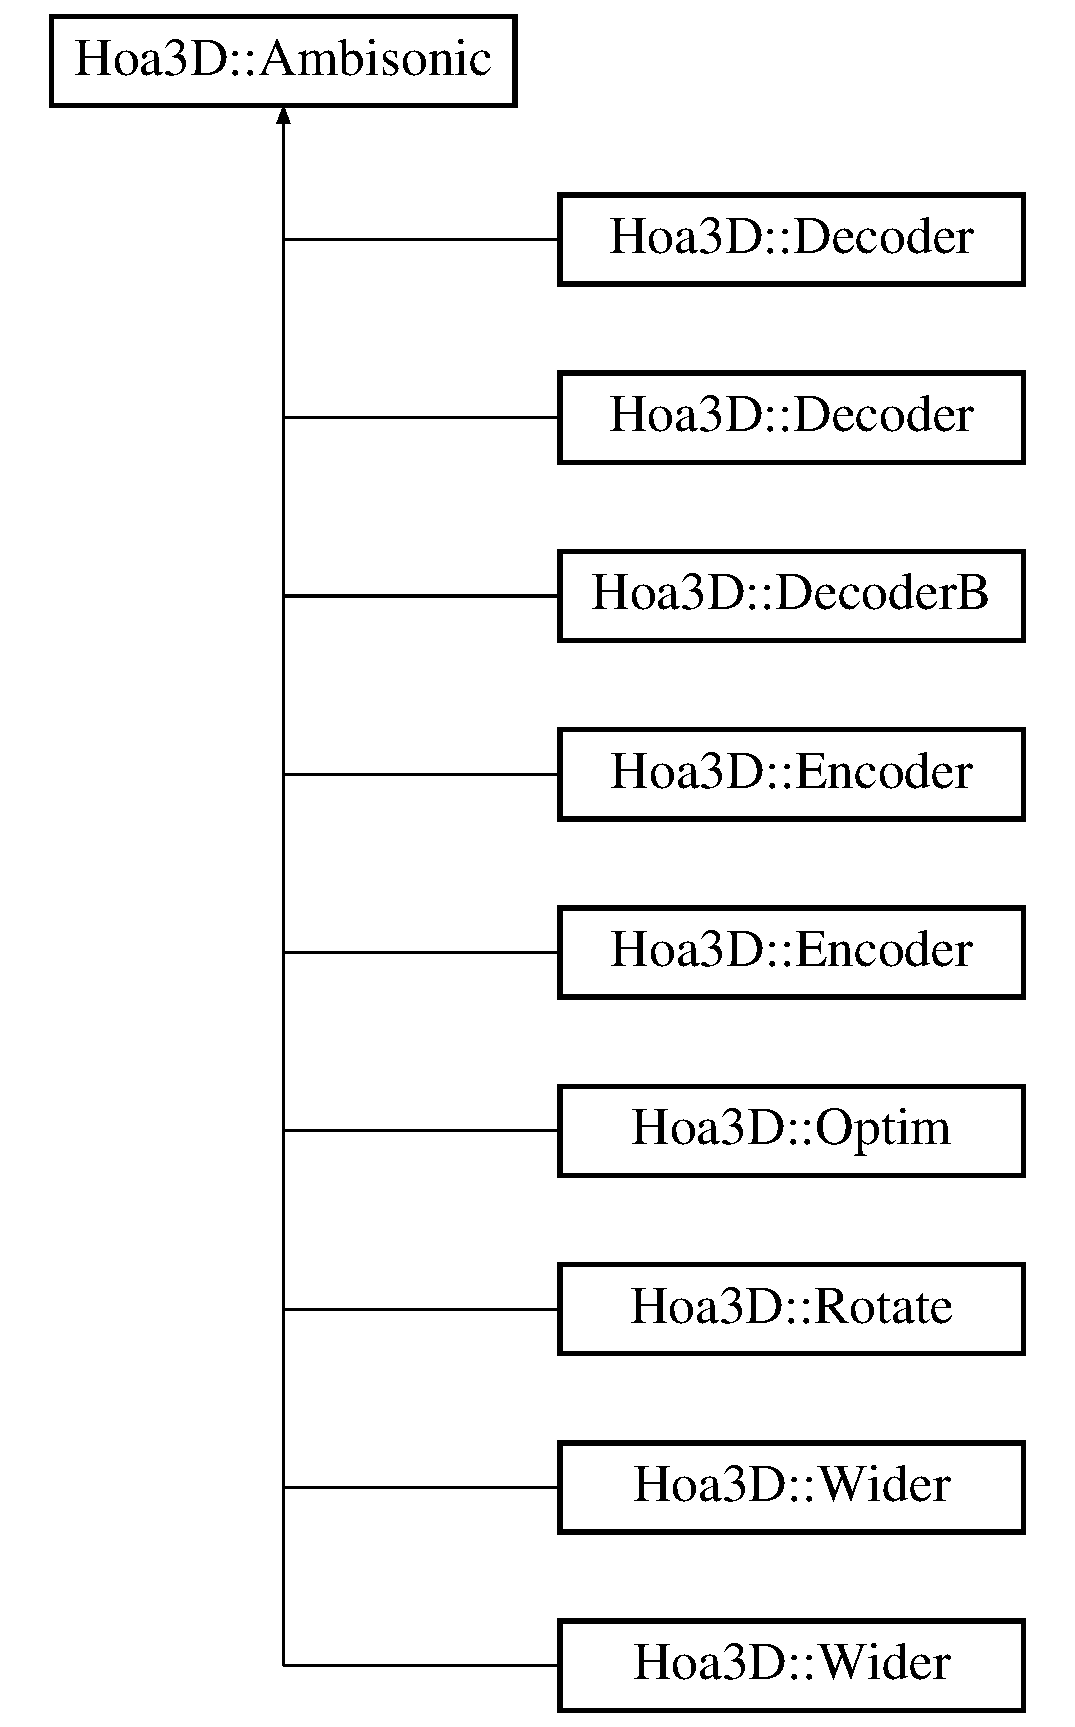
\includegraphics[height=2.000000cm]{class_hoa3_d_1_1_ambisonic}
\end{center}
\end{figure}
\subsection*{Public Member Functions}
\begin{DoxyCompactItemize}
\item 
\hyperlink{class_hoa3_d_1_1_ambisonic_aedbcac4a5b11cec6738e1047ecee7e7b}{Ambisonic} (unsigned int order=1)
\begin{DoxyCompactList}\small\item\em The ambisonic constructor. \end{DoxyCompactList}\item 
\hyperlink{class_hoa3_d_1_1_ambisonic_a082fc2e3f9910703ddb49b9a478329bf}{$\sim$\-Ambisonic} ()
\item 
long \hyperlink{class_hoa3_d_1_1_ambisonic_a677405a1c3aa359753bd675d4614e7da}{get\-Order} ()
\item 
long \hyperlink{class_hoa3_d_1_1_ambisonic_aa9d613f38e6876326201995a5a415410}{get\-Number\-Of\-Harmonics} ()
\item 
long \hyperlink{class_hoa3_d_1_1_ambisonic_af03625afb9f21ef3574eafa8501129b4}{get\-Number\-Of\-Inputs} ()
\item 
long \hyperlink{class_hoa3_d_1_1_ambisonic_a126ed3be1aa3d155f56ca75ca3d69de5}{get\-Number\-Of\-Outputs} ()
\item 
long \hyperlink{class_hoa3_d_1_1_ambisonic_a3acaabfd013671c94e057e23eea1d068}{get\-Harmonic\-Argument} (unsigned int index)
\begin{DoxyCompactList}\small\item\em Retrieve the argument of an harmonic. \end{DoxyCompactList}\item 
long \hyperlink{class_hoa3_d_1_1_ambisonic_a06ecceb7aef44cd7008fd8beaf8cf33e}{get\-Harmonic\-Band} (unsigned int index)
\begin{DoxyCompactList}\small\item\em Retrieve the band of an harmonic. \end{DoxyCompactList}\item 
std\-::string \hyperlink{class_hoa3_d_1_1_ambisonic_a1b4578538f4fd0d311102b2f3ec4dac6}{get\-Harmonics\-Name} (unsigned int index)
\begin{DoxyCompactList}\small\item\em Retrieve a good name for an harmonic. \end{DoxyCompactList}\end{DoxyCompactItemize}


\subsection{Detailed Description}
The ambisonic class. 

Most of the ambisonic classes inherit from this classe. It computes the number of harmonics, their indices and their orders depending of the decomposition order. etc... 

\subsection{Constructor \& Destructor Documentation}
\hypertarget{class_hoa3_d_1_1_ambisonic_aedbcac4a5b11cec6738e1047ecee7e7b}{\index{Hoa3\-D\-::\-Ambisonic@{Hoa3\-D\-::\-Ambisonic}!Ambisonic@{Ambisonic}}
\index{Ambisonic@{Ambisonic}!Hoa3D::Ambisonic@{Hoa3\-D\-::\-Ambisonic}}
\subsubsection[{Ambisonic}]{\setlength{\rightskip}{0pt plus 5cm}Ambisonic\-::\-Ambisonic (
\begin{DoxyParamCaption}
\item[{unsigned int}]{order = {\ttfamily 1}}
\end{DoxyParamCaption}
)}}\label{class_hoa3_d_1_1_ambisonic_aedbcac4a5b11cec6738e1047ecee7e7b}


The ambisonic constructor. 

The ambisonic constructor allocates and initializes the generale member values depending of a decomposition order. 
\begin{DoxyParams}{Parameters}
{\em order} & The order, must be at least 1. \\
\hline
\end{DoxyParams}
\hypertarget{class_hoa3_d_1_1_ambisonic_a082fc2e3f9910703ddb49b9a478329bf}{\index{Hoa3\-D\-::\-Ambisonic@{Hoa3\-D\-::\-Ambisonic}!$\sim$\-Ambisonic@{$\sim$\-Ambisonic}}
\index{$\sim$\-Ambisonic@{$\sim$\-Ambisonic}!Hoa3D::Ambisonic@{Hoa3\-D\-::\-Ambisonic}}
\subsubsection[{$\sim$\-Ambisonic}]{\setlength{\rightskip}{0pt plus 5cm}Ambisonic\-::$\sim$\-Ambisonic (
\begin{DoxyParamCaption}
{}
\end{DoxyParamCaption}
)}}\label{class_hoa3_d_1_1_ambisonic_a082fc2e3f9910703ddb49b9a478329bf}
The ambisonic destructor. 

\subsection{Member Function Documentation}
\hypertarget{class_hoa3_d_1_1_ambisonic_a3acaabfd013671c94e057e23eea1d068}{\index{Hoa3\-D\-::\-Ambisonic@{Hoa3\-D\-::\-Ambisonic}!get\-Harmonic\-Argument@{get\-Harmonic\-Argument}}
\index{get\-Harmonic\-Argument@{get\-Harmonic\-Argument}!Hoa3D::Ambisonic@{Hoa3\-D\-::\-Ambisonic}}
\subsubsection[{get\-Harmonic\-Argument}]{\setlength{\rightskip}{0pt plus 5cm}long Ambisonic\-::get\-Harmonic\-Argument (
\begin{DoxyParamCaption}
\item[{unsigned int}]{index}
\end{DoxyParamCaption}
)}}\label{class_hoa3_d_1_1_ambisonic_a3acaabfd013671c94e057e23eea1d068}


Retrieve the argument of an harmonic. 

The argument of an harmonic is in the range -\/band to band. The harmonics are sorted by their bands, from 0 to the decomposition order and, in each band, they are sorted by their arguments in the range -\/band to band. For the first bands, the harmonics arrangement is h\mbox{[}0, 0\mbox{]} h\mbox{[}1, -\/1\mbox{]} h\mbox{[}1, 0\mbox{]} h\mbox{[}1, 1\mbox{]} h\mbox{[}2, -\/2\mbox{]} h\mbox{[}2, -\/1\mbox{]} h\mbox{[}2, 0\mbox{]} h\mbox{[}2, 1\mbox{]} h\mbox{[}2, 2\mbox{]} etc. with h\mbox{[}band, argument\mbox{]}.


\begin{DoxyParams}{Parameters}
{\em index} & The global index of an harmonic. \\
\hline
\end{DoxyParams}
\begin{DoxyReturn}{Returns}
The method returns the argument of an harmonic or 0 if the harmonic does not exist. 
\end{DoxyReturn}
\begin{DoxySeeAlso}{See Also}
\hyperlink{class_hoa3_d_1_1_ambisonic_a06ecceb7aef44cd7008fd8beaf8cf33e}{get\-Harmonic\-Band()} 
\end{DoxySeeAlso}
\hypertarget{class_hoa3_d_1_1_ambisonic_a06ecceb7aef44cd7008fd8beaf8cf33e}{\index{Hoa3\-D\-::\-Ambisonic@{Hoa3\-D\-::\-Ambisonic}!get\-Harmonic\-Band@{get\-Harmonic\-Band}}
\index{get\-Harmonic\-Band@{get\-Harmonic\-Band}!Hoa3D::Ambisonic@{Hoa3\-D\-::\-Ambisonic}}
\subsubsection[{get\-Harmonic\-Band}]{\setlength{\rightskip}{0pt plus 5cm}long Ambisonic\-::get\-Harmonic\-Band (
\begin{DoxyParamCaption}
\item[{unsigned int}]{index}
\end{DoxyParamCaption}
)}}\label{class_hoa3_d_1_1_ambisonic_a06ecceb7aef44cd7008fd8beaf8cf33e}


Retrieve the band of an harmonic. 

The bands of the harmonics are in the range 0 to the decomposition order. Each band contains 2 $\ast$ band + 1 harmonics in the range -\/band to band. For the first bands, the harmonics arrangement is h\mbox{[}0, 0\mbox{]} h\mbox{[}1, -\/1\mbox{]} h\mbox{[}1, 0\mbox{]} h\mbox{[}1, 1\mbox{]} h\mbox{[}2, -\/2\mbox{]} h\mbox{[}2, -\/1\mbox{]} h\mbox{[}2, 0\mbox{]} h\mbox{[}2, 1\mbox{]} h\mbox{[}2, 2\mbox{]} etc. with h\mbox{[}band, argument\mbox{]}.


\begin{DoxyParams}{Parameters}
{\em index} & The global index of an harmonic. \\
\hline
\end{DoxyParams}
\begin{DoxyReturn}{Returns}
The method returns the band of an harmonic or 0 if the harmonic does not exist. 
\end{DoxyReturn}
\begin{DoxySeeAlso}{See Also}
\hyperlink{class_hoa3_d_1_1_ambisonic_a3acaabfd013671c94e057e23eea1d068}{get\-Harmonic\-Argument()} 
\end{DoxySeeAlso}
\hypertarget{class_hoa3_d_1_1_ambisonic_a1b4578538f4fd0d311102b2f3ec4dac6}{\index{Hoa3\-D\-::\-Ambisonic@{Hoa3\-D\-::\-Ambisonic}!get\-Harmonics\-Name@{get\-Harmonics\-Name}}
\index{get\-Harmonics\-Name@{get\-Harmonics\-Name}!Hoa3D::Ambisonic@{Hoa3\-D\-::\-Ambisonic}}
\subsubsection[{get\-Harmonics\-Name}]{\setlength{\rightskip}{0pt plus 5cm}std\-::string Ambisonic\-::get\-Harmonics\-Name (
\begin{DoxyParamCaption}
\item[{unsigned int}]{index}
\end{DoxyParamCaption}
)}}\label{class_hoa3_d_1_1_ambisonic_a1b4578538f4fd0d311102b2f3ec4dac6}


Retrieve a good name for an harmonic. 

Retrieve a good name for an harmonic.


\begin{DoxyParams}{Parameters}
{\em index} & The global index of an harmonic. \\
\hline
\end{DoxyParams}
\hypertarget{class_hoa3_d_1_1_ambisonic_aa9d613f38e6876326201995a5a415410}{\index{Hoa3\-D\-::\-Ambisonic@{Hoa3\-D\-::\-Ambisonic}!get\-Number\-Of\-Harmonics@{get\-Number\-Of\-Harmonics}}
\index{get\-Number\-Of\-Harmonics@{get\-Number\-Of\-Harmonics}!Hoa3D::Ambisonic@{Hoa3\-D\-::\-Ambisonic}}
\subsubsection[{get\-Number\-Of\-Harmonics}]{\setlength{\rightskip}{0pt plus 5cm}long Ambisonic\-::get\-Number\-Of\-Harmonics (
\begin{DoxyParamCaption}
{}
\end{DoxyParamCaption}
)}}\label{class_hoa3_d_1_1_ambisonic_aa9d613f38e6876326201995a5a415410}
Retrieve the number of harmonics. \hypertarget{class_hoa3_d_1_1_ambisonic_af03625afb9f21ef3574eafa8501129b4}{\index{Hoa3\-D\-::\-Ambisonic@{Hoa3\-D\-::\-Ambisonic}!get\-Number\-Of\-Inputs@{get\-Number\-Of\-Inputs}}
\index{get\-Number\-Of\-Inputs@{get\-Number\-Of\-Inputs}!Hoa3D::Ambisonic@{Hoa3\-D\-::\-Ambisonic}}
\subsubsection[{get\-Number\-Of\-Inputs}]{\setlength{\rightskip}{0pt plus 5cm}long Ambisonic\-::get\-Number\-Of\-Inputs (
\begin{DoxyParamCaption}
{}
\end{DoxyParamCaption}
)}}\label{class_hoa3_d_1_1_ambisonic_af03625afb9f21ef3574eafa8501129b4}
Retrieve the number of inputs. \hypertarget{class_hoa3_d_1_1_ambisonic_a126ed3be1aa3d155f56ca75ca3d69de5}{\index{Hoa3\-D\-::\-Ambisonic@{Hoa3\-D\-::\-Ambisonic}!get\-Number\-Of\-Outputs@{get\-Number\-Of\-Outputs}}
\index{get\-Number\-Of\-Outputs@{get\-Number\-Of\-Outputs}!Hoa3D::Ambisonic@{Hoa3\-D\-::\-Ambisonic}}
\subsubsection[{get\-Number\-Of\-Outputs}]{\setlength{\rightskip}{0pt plus 5cm}long Ambisonic\-::get\-Number\-Of\-Outputs (
\begin{DoxyParamCaption}
{}
\end{DoxyParamCaption}
)}}\label{class_hoa3_d_1_1_ambisonic_a126ed3be1aa3d155f56ca75ca3d69de5}
Retrieve the number of outputs. \hypertarget{class_hoa3_d_1_1_ambisonic_a677405a1c3aa359753bd675d4614e7da}{\index{Hoa3\-D\-::\-Ambisonic@{Hoa3\-D\-::\-Ambisonic}!get\-Order@{get\-Order}}
\index{get\-Order@{get\-Order}!Hoa3D::Ambisonic@{Hoa3\-D\-::\-Ambisonic}}
\subsubsection[{get\-Order}]{\setlength{\rightskip}{0pt plus 5cm}long Ambisonic\-::get\-Order (
\begin{DoxyParamCaption}
{}
\end{DoxyParamCaption}
)}}\label{class_hoa3_d_1_1_ambisonic_a677405a1c3aa359753bd675d4614e7da}
Retrieve the decomposition order. 

The documentation for this class was generated from the following files\-:\begin{DoxyCompactItemize}
\item 
/\-Users/\-Pierre/\-Source\-Tree/\-Hoa\-Library/\-Sources/hoa\-Ambisonics/Hoa3\-D\-Ambisonic.\-h\item 
/\-Users/\-Pierre/\-Source\-Tree/\-Hoa\-Library/\-Sources/hoa\-Ambisonics/Hoa3\-D\-Ambisonic.\-cpp\end{DoxyCompactItemize}

\hypertarget{class_ambisonic_projector}{\section{Ambisonic\-Projector Class Reference}
\label{class_ambisonic_projector}\index{Ambisonic\-Projector@{Ambisonic\-Projector}}
}


{\ttfamily \#include $<$Ambisonic\-Projector.\-h$>$}

Inheritance diagram for Ambisonic\-Projector\-:\begin{figure}[H]
\begin{center}
\leavevmode
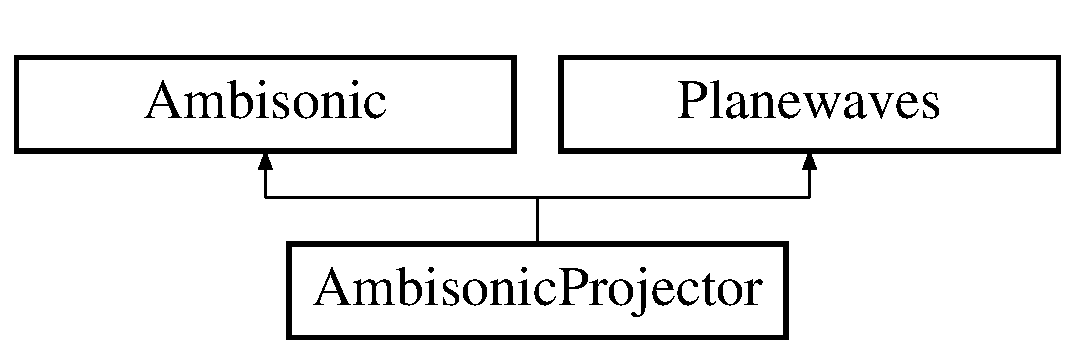
\includegraphics[height=2.000000cm]{class_ambisonic_projector}
\end{center}
\end{figure}
\subsection*{Public Member Functions}
\begin{DoxyCompactItemize}
\item 
\hyperlink{class_ambisonic_projector_a611af47413099ddc30e7075953c9a038}{Ambisonic\-Projector} (long an\-Order=1, long a\-Number\-Of\-Loudspeakers=3, long a\-Vector\-Size=0)
\end{DoxyCompactItemize}


\subsection{Detailed Description}
Hoa\-Library \-: A High Order Ambisonics Library Copyright (c) 2012-\/2013 Julien Colafrancesco, Pierre Guillot, Eliott Paris, C\-I\-C\-M, Universite Paris-\/8. All rights reserved.

Website \-: \href{http://www.mshparisnord.fr/hoalibrary/}{\tt http\-://www.\-mshparisnord.\-fr/hoalibrary/} Contacts \-: \href{mailto:cicm.mshparisnord@gmail.com}{\tt cicm.\-mshparisnord@gmail.\-com}

Redistribution and use in source and binary forms, with or without modification, are permitted provided that the following conditions are met\-:


\begin{DoxyItemize}
\item Redistributions may not be sold, nor may they be used in a commercial product or activity.
\item Redistributions of source code must retain the above copyright notice, this list of conditions and the following disclaimer.
\item Redistributions in binary form must reproduce the above copyright notice, this list of conditions and the following disclaimer in the documentation and/or other materials provided with the distribution.
\item Neither the name of the C\-I\-C\-M nor the names of its contributors may be used to endorse or promote products derived from this software without specific prior written permission.
\end{DoxyItemize}

T\-H\-I\-S S\-O\-F\-T\-W\-A\-R\-E I\-S P\-R\-O\-V\-I\-D\-E\-D B\-Y T\-H\-E C\-O\-P\-Y\-R\-I\-G\-H\-T H\-O\-L\-D\-E\-R\-S A\-N\-D C\-O\-N\-T\-R\-I\-B\-U\-T\-O\-R\-S \char`\"{}\-A\-S I\-S\char`\"{} A\-N\-D A\-N\-Y E\-X\-P\-R\-E\-S\-S O\-R I\-M\-P\-L\-I\-E\-D W\-A\-R\-R\-A\-N\-T\-I\-E\-S, I\-N\-C\-L\-U\-D\-I\-N\-G, B\-U\-T N\-O\-T L\-I\-M\-I\-T\-E\-D T\-O, T\-H\-E I\-M\-P\-L\-I\-E\-D W\-A\-R\-R\-A\-N\-T\-I\-E\-S O\-F M\-E\-R\-C\-H\-A\-N\-T\-A\-B\-I\-L\-I\-T\-Y A\-N\-D F\-I\-T\-N\-E\-S\-S F\-O\-R A P\-A\-R\-T\-I\-C\-U\-L\-A\-R P\-U\-R\-P\-O\-S\-E A\-R\-E D\-I\-S\-C\-L\-A\-I\-M\-E\-D. I\-N N\-O E\-V\-E\-N\-T S\-H\-A\-L\-L T\-H\-E C\-O\-P\-Y\-R\-I\-G\-H\-T H\-O\-L\-D\-E\-R O\-R C\-O\-N\-T\-R\-I\-B\-U\-T\-O\-R\-S B\-E L\-I\-A\-B\-L\-E F\-O\-R A\-N\-Y D\-I\-R\-E\-C\-T, I\-N\-D\-I\-R\-E\-C\-T, I\-N\-C\-I\-D\-E\-N\-T\-A\-L, S\-P\-E\-C\-I\-A\-L, E\-X\-E\-M\-P\-L\-A\-R\-Y, O\-R C\-O\-N\-S\-E\-Q\-U\-E\-N\-T\-I\-A\-L D\-A\-M\-A\-G\-E\-S (I\-N\-C\-L\-U\-D\-I\-N\-G, B\-U\-T N\-O\-T L\-I\-M\-I\-T\-E\-D T\-O, P\-R\-O\-C\-U\-R\-E\-M\-E\-N\-T O\-F S\-U\-B\-S\-T\-I\-T\-U\-T\-E G\-O\-O\-D\-S O\-R S\-E\-R\-V\-I\-C\-E\-S; L\-O\-S\-S O\-F U\-S\-E, D\-A\-T\-A, O\-R P\-R\-O\-F\-I\-T\-S; O\-R B\-U\-S\-I\-N\-E\-S\-S I\-N\-T\-E\-R\-R\-U\-P\-T\-I\-O\-N) H\-O\-W\-E\-V\-E\-R C\-A\-U\-S\-E\-D A\-N\-D O\-N A\-N\-Y T\-H\-E\-O\-R\-Y O\-F L\-I\-A\-B\-I\-L\-I\-T\-Y, W\-H\-E\-T\-H\-E\-R I\-N C\-O\-N\-T\-R\-A\-C\-T, S\-T\-R\-I\-C\-T L\-I\-A\-B\-I\-L\-I\-T\-Y, O\-R T\-O\-R\-T (I\-N\-C\-L\-U\-D\-I\-N\-G N\-E\-G\-L\-I\-G\-E\-N\-C\-E O\-R O\-T\-H\-E\-R\-W\-I\-S\-E) A\-R\-I\-S\-I\-N\-G I\-N A\-N\-Y W\-A\-Y O\-U\-T O\-F T\-H\-E U\-S\-E O\-F T\-H\-I\-S S\-O\-F\-T\-W\-A\-R\-E, E\-V\-E\-N I\-F A\-D\-V\-I\-S\-E\-D O\-F T\-H\-E P\-O\-S\-S\-I\-B\-I\-L\-I\-T\-Y O\-F S\-U\-C\-H D\-A\-M\-A\-G\-E. 

Definition at line 32 of file Ambisonic\-Projector.\-h.



\subsection{Constructor \& Destructor Documentation}
\hypertarget{class_ambisonic_projector_a611af47413099ddc30e7075953c9a038}{\index{Ambisonic\-Projector@{Ambisonic\-Projector}!Ambisonic\-Projector@{Ambisonic\-Projector}}
\index{Ambisonic\-Projector@{Ambisonic\-Projector}!AmbisonicProjector@{Ambisonic\-Projector}}
\subsubsection[{Ambisonic\-Projector}]{\setlength{\rightskip}{0pt plus 5cm}Ambisonic\-Projector\-::\-Ambisonic\-Projector (
\begin{DoxyParamCaption}
\item[{long}]{an\-Order = {\ttfamily 1}, }
\item[{long}]{a\-Number\-Of\-Loudspeakers = {\ttfamily 3}, }
\item[{long}]{a\-Vector\-Size = {\ttfamily 0}}
\end{DoxyParamCaption}
)}}\label{class_ambisonic_projector_a611af47413099ddc30e7075953c9a038}
Hoa\-Library \-: A High Order Ambisonics Library Copyright (c) 2012-\/2013 Julien Colafrancesco, Pierre Guillot, Eliott Paris, C\-I\-C\-M, Universite Paris-\/8. All rights reserved.

Website \-: \href{http://www.mshparisnord.fr/hoalibrary/}{\tt http\-://www.\-mshparisnord.\-fr/hoalibrary/} Contacts \-: \href{mailto:cicm.mshparisnord@gmail.com}{\tt cicm.\-mshparisnord@gmail.\-com}

Redistribution and use in source and binary forms, with or without modification, are permitted provided that the following conditions are met\-:


\begin{DoxyItemize}
\item Redistributions may not be sold, nor may they be used in a commercial product or activity.
\item Redistributions of source code must retain the above copyright notice, this list of conditions and the following disclaimer.
\item Redistributions in binary form must reproduce the above copyright notice, this list of conditions and the following disclaimer in the documentation and/or other materials provided with the distribution.
\item Neither the name of the C\-I\-C\-M nor the names of its contributors may be used to endorse or promote products derived from this software without specific prior written permission.
\end{DoxyItemize}

T\-H\-I\-S S\-O\-F\-T\-W\-A\-R\-E I\-S P\-R\-O\-V\-I\-D\-E\-D B\-Y T\-H\-E C\-O\-P\-Y\-R\-I\-G\-H\-T H\-O\-L\-D\-E\-R\-S A\-N\-D C\-O\-N\-T\-R\-I\-B\-U\-T\-O\-R\-S \char`\"{}\-A\-S I\-S\char`\"{} A\-N\-D A\-N\-Y E\-X\-P\-R\-E\-S\-S O\-R I\-M\-P\-L\-I\-E\-D W\-A\-R\-R\-A\-N\-T\-I\-E\-S, I\-N\-C\-L\-U\-D\-I\-N\-G, B\-U\-T N\-O\-T L\-I\-M\-I\-T\-E\-D T\-O, T\-H\-E I\-M\-P\-L\-I\-E\-D W\-A\-R\-R\-A\-N\-T\-I\-E\-S O\-F M\-E\-R\-C\-H\-A\-N\-T\-A\-B\-I\-L\-I\-T\-Y A\-N\-D F\-I\-T\-N\-E\-S\-S F\-O\-R A P\-A\-R\-T\-I\-C\-U\-L\-A\-R P\-U\-R\-P\-O\-S\-E A\-R\-E D\-I\-S\-C\-L\-A\-I\-M\-E\-D. I\-N N\-O E\-V\-E\-N\-T S\-H\-A\-L\-L T\-H\-E C\-O\-P\-Y\-R\-I\-G\-H\-T H\-O\-L\-D\-E\-R O\-R C\-O\-N\-T\-R\-I\-B\-U\-T\-O\-R\-S B\-E L\-I\-A\-B\-L\-E F\-O\-R A\-N\-Y D\-I\-R\-E\-C\-T, I\-N\-D\-I\-R\-E\-C\-T, I\-N\-C\-I\-D\-E\-N\-T\-A\-L, S\-P\-E\-C\-I\-A\-L, E\-X\-E\-M\-P\-L\-A\-R\-Y, O\-R C\-O\-N\-S\-E\-Q\-U\-E\-N\-T\-I\-A\-L D\-A\-M\-A\-G\-E\-S (I\-N\-C\-L\-U\-D\-I\-N\-G, B\-U\-T N\-O\-T L\-I\-M\-I\-T\-E\-D T\-O, P\-R\-O\-C\-U\-R\-E\-M\-E\-N\-T O\-F S\-U\-B\-S\-T\-I\-T\-U\-T\-E G\-O\-O\-D\-S O\-R S\-E\-R\-V\-I\-C\-E\-S; L\-O\-S\-S O\-F U\-S\-E, D\-A\-T\-A, O\-R P\-R\-O\-F\-I\-T\-S; O\-R B\-U\-S\-I\-N\-E\-S\-S I\-N\-T\-E\-R\-R\-U\-P\-T\-I\-O\-N) H\-O\-W\-E\-V\-E\-R C\-A\-U\-S\-E\-D A\-N\-D O\-N A\-N\-Y T\-H\-E\-O\-R\-Y O\-F L\-I\-A\-B\-I\-L\-I\-T\-Y, W\-H\-E\-T\-H\-E\-R I\-N C\-O\-N\-T\-R\-A\-C\-T, S\-T\-R\-I\-C\-T L\-I\-A\-B\-I\-L\-I\-T\-Y, O\-R T\-O\-R\-T (I\-N\-C\-L\-U\-D\-I\-N\-G N\-E\-G\-L\-I\-G\-E\-N\-C\-E O\-R O\-T\-H\-E\-R\-W\-I\-S\-E) A\-R\-I\-S\-I\-N\-G I\-N A\-N\-Y W\-A\-Y O\-U\-T O\-F T\-H\-E U\-S\-E O\-F T\-H\-I\-S S\-O\-F\-T\-W\-A\-R\-E, E\-V\-E\-N I\-F A\-D\-V\-I\-S\-E\-D O\-F T\-H\-E P\-O\-S\-S\-I\-B\-I\-L\-I\-T\-Y O\-F S\-U\-C\-H D\-A\-M\-A\-G\-E. 

Definition at line 28 of file Ambisonic\-Projector.\-cpp.



The documentation for this class was generated from the following files\-:\begin{DoxyCompactItemize}
\item 
/\-Users/elioton/\-Documents/programmation/\-C\-I\-C\-M/source\-Tree/\-Hoa\-Library/\-Sources/hoa\-Projector/Ambisonic\-Projector.\-h\item 
/\-Users/elioton/\-Documents/programmation/\-C\-I\-C\-M/source\-Tree/\-Hoa\-Library/\-Sources/hoa\-Projector/Ambisonic\-Projector.\-cpp\end{DoxyCompactItemize}

\hypertarget{class_ambisonic_recomposer}{\section{Ambisonic\-Recomposer Class Reference}
\label{class_ambisonic_recomposer}\index{Ambisonic\-Recomposer@{Ambisonic\-Recomposer}}
}
Inheritance diagram for Ambisonic\-Recomposer\-:\begin{figure}[H]
\begin{center}
\leavevmode
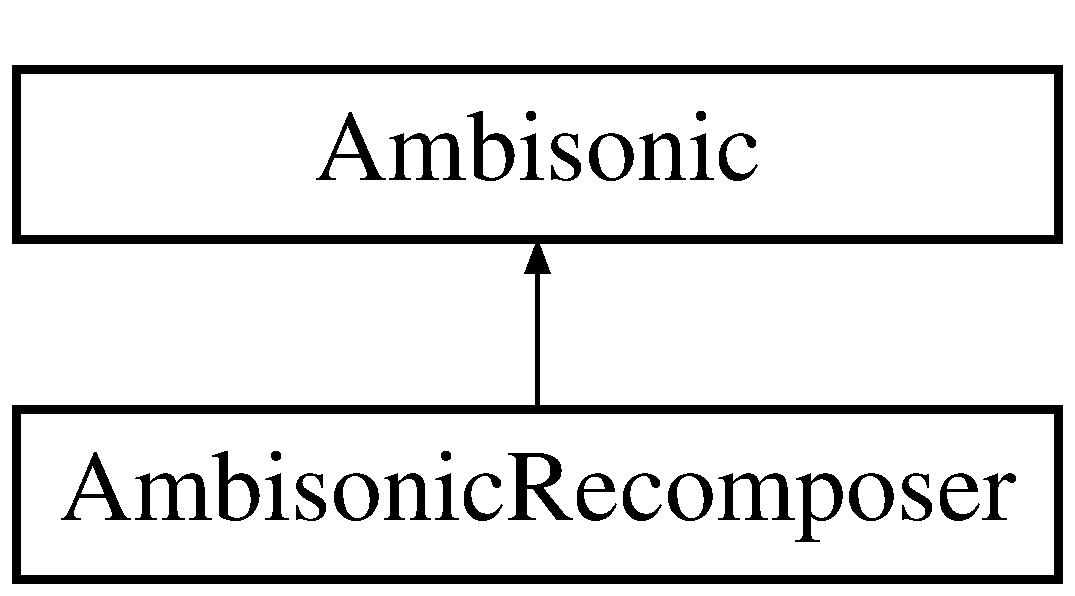
\includegraphics[height=2.000000cm]{class_ambisonic_recomposer}
\end{center}
\end{figure}
\subsection*{Additional Inherited Members}


\subsection{Detailed Description}


Definition at line 42 of file Ambisonic\-Recomposer.\-h.



The documentation for this class was generated from the following files\-:\begin{DoxyCompactItemize}
\item 
/\-Users/\-Pierre/\-Source\-Tree/\-Hoa\-Library/\-Sources/hoa\-Recomposer/Ambisonic\-Recomposer.\-h\item 
/\-Users/\-Pierre/\-Source\-Tree/\-Hoa\-Library/\-Sources/hoa\-Recomposer/Ambisonic\-Recomposer.\-cpp\end{DoxyCompactItemize}

\hypertarget{class_ambisonics_binaural}{\section{Ambisonics\-Binaural Class Reference}
\label{class_ambisonics_binaural}\index{Ambisonics\-Binaural@{Ambisonics\-Binaural}}
}
Inheritance diagram for Ambisonics\-Binaural\-:\begin{figure}[H]
\begin{center}
\leavevmode
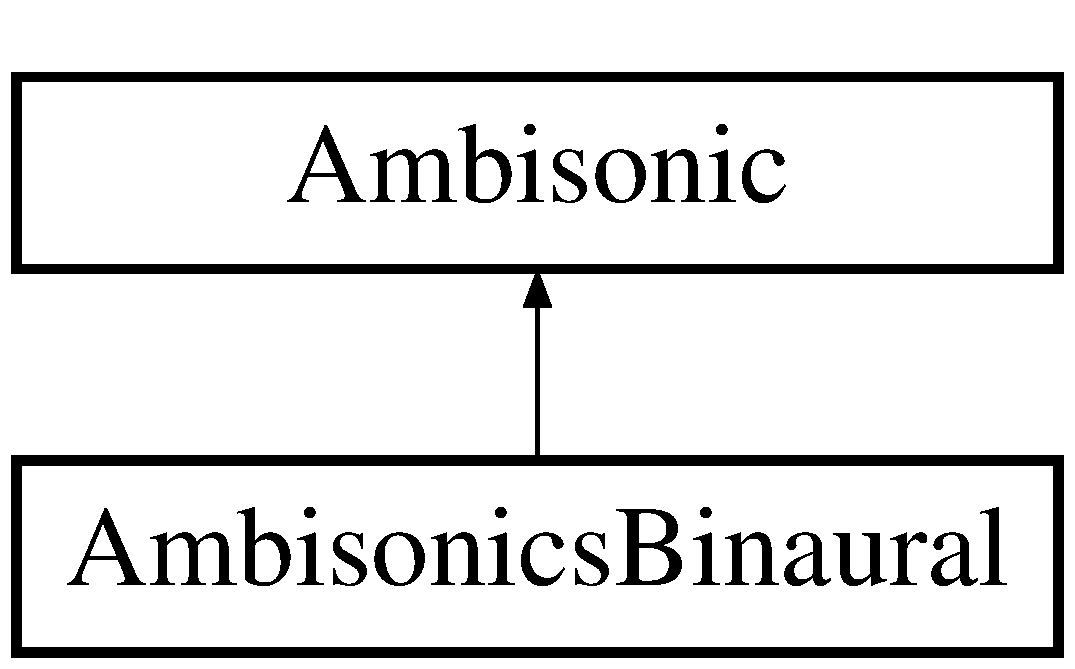
\includegraphics[height=2.000000cm]{class_ambisonics_binaural}
\end{center}
\end{figure}
\subsection*{Public Member Functions}
\begin{DoxyCompactItemize}
\item 
\hyperlink{class_ambisonics_binaural_aa3154f11cb7a385b09a743c5e46ee2e9}{Ambisonics\-Binaural} (long an\-Order=1, std\-::string a\-Root\-Path=\char`\"{}\char`\"{}, long a\-Pinnae\-Size=Hoa\-\_\-\-Small, double a\-Sampling\-Rate=44100, long a\-Vector\-Size=0)
\end{DoxyCompactItemize}


\subsection{Detailed Description}


Definition at line 37 of file Ambisonics\-Binaural.\-h.



\subsection{Constructor \& Destructor Documentation}
\hypertarget{class_ambisonics_binaural_aa3154f11cb7a385b09a743c5e46ee2e9}{\index{Ambisonics\-Binaural@{Ambisonics\-Binaural}!Ambisonics\-Binaural@{Ambisonics\-Binaural}}
\index{Ambisonics\-Binaural@{Ambisonics\-Binaural}!AmbisonicsBinaural@{Ambisonics\-Binaural}}
\subsubsection[{Ambisonics\-Binaural}]{\setlength{\rightskip}{0pt plus 5cm}Ambisonics\-Binaural\-::\-Ambisonics\-Binaural (
\begin{DoxyParamCaption}
\item[{long}]{an\-Order = {\ttfamily 1}, }
\item[{std\-::string}]{a\-Root\-Path = {\ttfamily \char`\"{}\char`\"{}}, }
\item[{long}]{a\-Pinnae\-Size = {\ttfamily Hoa\-\_\-Small}, }
\item[{double}]{a\-Sampling\-Rate = {\ttfamily 44100}, }
\item[{long}]{a\-Vector\-Size = {\ttfamily 0}}
\end{DoxyParamCaption}
)}}\label{class_ambisonics_binaural_aa3154f11cb7a385b09a743c5e46ee2e9}
Hoa\-Library \-: A High Order Ambisonics Library Copyright (c) 2012-\/2013 Julien Colafrancesco, Pierre Guillot, Eliott Paris, C\-I\-C\-M, Universite Paris-\/8. All rights reserved.

Website \-: \href{http://www.mshparisnord.fr/hoalibrary/}{\tt http\-://www.\-mshparisnord.\-fr/hoalibrary/} Contacts \-: \href{mailto:cicm.mshparisnord@gmail.com}{\tt cicm.\-mshparisnord@gmail.\-com}

Redistribution and use in source and binary forms, with or without modification, are permitted provided that the following conditions are met\-:


\begin{DoxyItemize}
\item Redistributions may not be sold, nor may they be used in a commercial product or activity.
\item Redistributions of source code must retain the above copyright notice, this list of conditions and the following disclaimer.
\item Redistributions in binary form must reproduce the above copyright notice, this list of conditions and the following disclaimer in the documentation and/or other materials provided with the distribution.
\item Neither the name of the C\-I\-C\-M nor the names of its contributors may be used to endorse or promote products derived from this software without specific prior written permission.
\end{DoxyItemize}

T\-H\-I\-S S\-O\-F\-T\-W\-A\-R\-E I\-S P\-R\-O\-V\-I\-D\-E\-D B\-Y T\-H\-E C\-O\-P\-Y\-R\-I\-G\-H\-T H\-O\-L\-D\-E\-R\-S A\-N\-D C\-O\-N\-T\-R\-I\-B\-U\-T\-O\-R\-S \char`\"{}\-A\-S I\-S\char`\"{} A\-N\-D A\-N\-Y E\-X\-P\-R\-E\-S\-S O\-R I\-M\-P\-L\-I\-E\-D W\-A\-R\-R\-A\-N\-T\-I\-E\-S, I\-N\-C\-L\-U\-D\-I\-N\-G, B\-U\-T N\-O\-T L\-I\-M\-I\-T\-E\-D T\-O, T\-H\-E I\-M\-P\-L\-I\-E\-D W\-A\-R\-R\-A\-N\-T\-I\-E\-S O\-F M\-E\-R\-C\-H\-A\-N\-T\-A\-B\-I\-L\-I\-T\-Y A\-N\-D F\-I\-T\-N\-E\-S\-S F\-O\-R A P\-A\-R\-T\-I\-C\-U\-L\-A\-R P\-U\-R\-P\-O\-S\-E A\-R\-E D\-I\-S\-C\-L\-A\-I\-M\-E\-D. I\-N N\-O E\-V\-E\-N\-T S\-H\-A\-L\-L T\-H\-E C\-O\-P\-Y\-R\-I\-G\-H\-T H\-O\-L\-D\-E\-R O\-R C\-O\-N\-T\-R\-I\-B\-U\-T\-O\-R\-S B\-E L\-I\-A\-B\-L\-E F\-O\-R A\-N\-Y D\-I\-R\-E\-C\-T, I\-N\-D\-I\-R\-E\-C\-T, I\-N\-C\-I\-D\-E\-N\-T\-A\-L, S\-P\-E\-C\-I\-A\-L, E\-X\-E\-M\-P\-L\-A\-R\-Y, O\-R C\-O\-N\-S\-E\-Q\-U\-E\-N\-T\-I\-A\-L D\-A\-M\-A\-G\-E\-S (I\-N\-C\-L\-U\-D\-I\-N\-G, B\-U\-T N\-O\-T L\-I\-M\-I\-T\-E\-D T\-O, P\-R\-O\-C\-U\-R\-E\-M\-E\-N\-T O\-F S\-U\-B\-S\-T\-I\-T\-U\-T\-E G\-O\-O\-D\-S O\-R S\-E\-R\-V\-I\-C\-E\-S; L\-O\-S\-S O\-F U\-S\-E, D\-A\-T\-A, O\-R P\-R\-O\-F\-I\-T\-S; O\-R B\-U\-S\-I\-N\-E\-S\-S I\-N\-T\-E\-R\-R\-U\-P\-T\-I\-O\-N) H\-O\-W\-E\-V\-E\-R C\-A\-U\-S\-E\-D A\-N\-D O\-N A\-N\-Y T\-H\-E\-O\-R\-Y O\-F L\-I\-A\-B\-I\-L\-I\-T\-Y, W\-H\-E\-T\-H\-E\-R I\-N C\-O\-N\-T\-R\-A\-C\-T, S\-T\-R\-I\-C\-T L\-I\-A\-B\-I\-L\-I\-T\-Y, O\-R T\-O\-R\-T (I\-N\-C\-L\-U\-D\-I\-N\-G N\-E\-G\-L\-I\-G\-E\-N\-C\-E O\-R O\-T\-H\-E\-R\-W\-I\-S\-E) A\-R\-I\-S\-I\-N\-G I\-N A\-N\-Y W\-A\-Y O\-U\-T O\-F T\-H\-E U\-S\-E O\-F T\-H\-I\-S S\-O\-F\-T\-W\-A\-R\-E, E\-V\-E\-N I\-F A\-D\-V\-I\-S\-E\-D O\-F T\-H\-E P\-O\-S\-S\-I\-B\-I\-L\-I\-T\-Y O\-F S\-U\-C\-H D\-A\-M\-A\-G\-E. 

Definition at line 29 of file Ambisonics\-Binaural.\-cpp.



The documentation for this class was generated from the following files\-:\begin{DoxyCompactItemize}
\item 
/\-Users/elioton/\-Documents/programmation/\-C\-I\-C\-M/source\-Tree/\-Hoa\-Library/\-Sources/hoa\-Binaural/Ambisonics\-Binaural.\-h\item 
/\-Users/elioton/\-Documents/programmation/\-C\-I\-C\-M/source\-Tree/\-Hoa\-Library/\-Sources/hoa\-Binaural/Ambisonics\-Binaural.\-cpp\end{DoxyCompactItemize}

\hypertarget{class_ambisonics_meter}{\section{Ambisonics\-Meter Class Reference}
\label{class_ambisonics_meter}\index{Ambisonics\-Meter@{Ambisonics\-Meter}}
}


{\ttfamily \#include $<$Ambisonics\-Meter.\-h$>$}

Inheritance diagram for Ambisonics\-Meter\-:\begin{figure}[H]
\begin{center}
\leavevmode
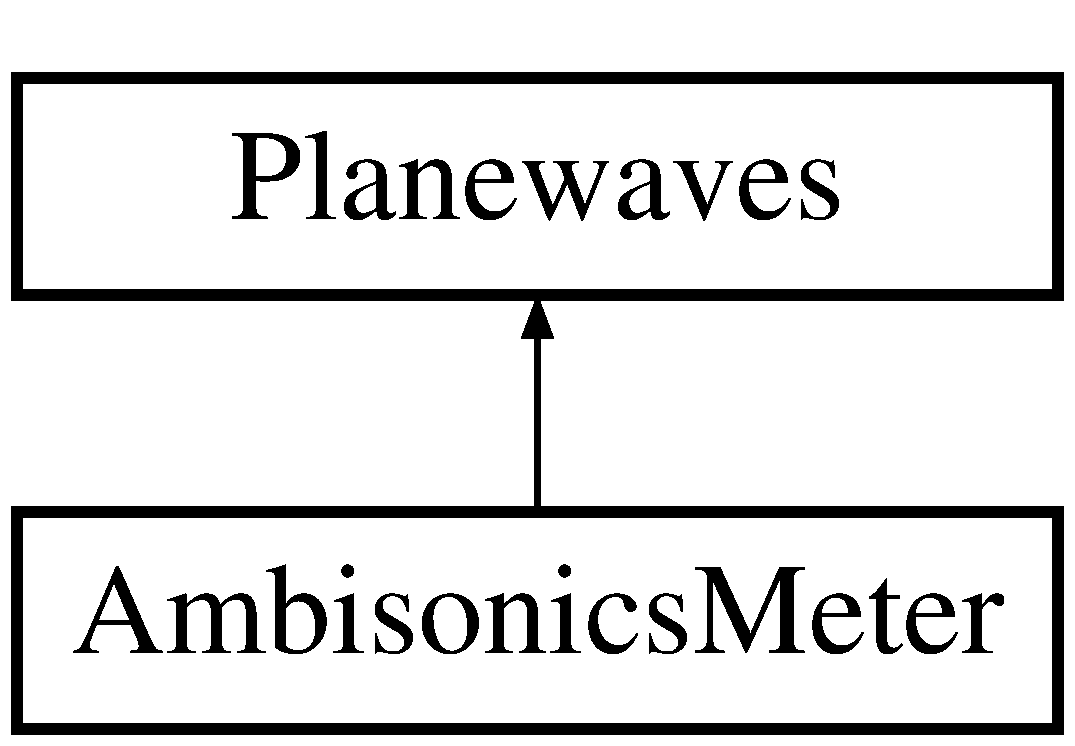
\includegraphics[height=2.000000cm]{class_ambisonics_meter}
\end{center}
\end{figure}
\subsection*{Public Member Functions}
\begin{DoxyCompactItemize}
\item 
\hyperlink{class_ambisonics_meter_ab6652775a732fc5d190101e5673c6758}{Ambisonics\-Meter} (long a\-Number\-Of\-Channel=1, long a\-Vector\-Size=0, double a\-Sampling\-Rate=44100.)
\item 
\hypertarget{class_ambisonics_meter_a67dcdc08682898d4460cf8e04f53a201}{void {\bfseries set\-Number\-Of\-Loudspeakers} (long a\-Number\-Of\-Channels)}\label{class_ambisonics_meter_a67dcdc08682898d4460cf8e04f53a201}

\item 
\hypertarget{class_ambisonics_meter_a14720821cf28453bc1609a234121c040}{void {\bfseries set\-Vector\-Size} (long a\-Vector\-Size)}\label{class_ambisonics_meter_a14720821cf28453bc1609a234121c040}

\item 
\hypertarget{class_ambisonics_meter_a991f4c9b08bf47e0eb10fda9e907f511}{void {\bfseries set\-Loudspeaker\-Angle\-Degrees} (long an\-Index, double an\-Angle)}\label{class_ambisonics_meter_a991f4c9b08bf47e0eb10fda9e907f511}

\item 
\hypertarget{class_ambisonics_meter_a58425860d8afb4eb62328833e68baf12}{void {\bfseries set\-Loudspeaker\-Angles\-Degrees} (long a\-Size, double $\ast$angles)}\label{class_ambisonics_meter_a58425860d8afb4eb62328833e68baf12}

\item 
\hypertarget{class_ambisonics_meter_a15bbfeebc227c01a4041316905e051c7}{double {\bfseries get\-Loudspeaker\-Peaks} (long an\-Index)}\label{class_ambisonics_meter_a15bbfeebc227c01a4041316905e051c7}

\item 
\hypertarget{class_ambisonics_meter_a2a1f8138c0b030eeb3f83a536c72e6e4}{double {\bfseries get\-Loudspeaker\-Energy} (long an\-Index)}\label{class_ambisonics_meter_a2a1f8138c0b030eeb3f83a536c72e6e4}

\item 
\hypertarget{class_ambisonics_meter_a73f0f5db0e7e5e15080d907cddc48e98}{double {\bfseries get\-Energy\-Vector\-Abscissa} ()}\label{class_ambisonics_meter_a73f0f5db0e7e5e15080d907cddc48e98}

\item 
\hypertarget{class_ambisonics_meter_a737f7cf7c2392a3caa50fc79daad1500}{double {\bfseries get\-Energy\-Vector\-Ordinate} ()}\label{class_ambisonics_meter_a737f7cf7c2392a3caa50fc79daad1500}

\item 
\hypertarget{class_ambisonics_meter_a597186413fff3df7e5ee2f82fd0c497a}{double {\bfseries get\-Energy\-Vector\-Angle} ()}\label{class_ambisonics_meter_a597186413fff3df7e5ee2f82fd0c497a}

\item 
\hypertarget{class_ambisonics_meter_a0ed4c04a207ef485252c9075f691be35}{double {\bfseries get\-Energy\-Vector\-Radius} ()}\label{class_ambisonics_meter_a0ed4c04a207ef485252c9075f691be35}

\item 
\hypertarget{class_ambisonics_meter_a1f4ec2a7672144bbeebfedc398e77439}{double {\bfseries get\-Velocity\-Vector\-Abscissa} ()}\label{class_ambisonics_meter_a1f4ec2a7672144bbeebfedc398e77439}

\item 
\hypertarget{class_ambisonics_meter_ab34bc7eff55c357550f05b2852eb6840}{double {\bfseries get\-Velocity\-Vector\-Ordinate} ()}\label{class_ambisonics_meter_ab34bc7eff55c357550f05b2852eb6840}

\item 
\hypertarget{class_ambisonics_meter_a937efec3de37d9702acf18b2b1b00109}{double {\bfseries get\-Velocity\-Vector\-Angle} ()}\label{class_ambisonics_meter_a937efec3de37d9702acf18b2b1b00109}

\item 
\hypertarget{class_ambisonics_meter_a48578aa4790dc7063e9ecb2d37dc66ba}{double {\bfseries get\-Velocity\-Vector\-Radius} ()}\label{class_ambisonics_meter_a48578aa4790dc7063e9ecb2d37dc66ba}

\item 
\hypertarget{class_ambisonics_meter_ad1b0981516635b7773383b498f2a9b39}{double {\bfseries get\-Loudspeaker\-Angle\-Mapped} (long an\-Index)}\label{class_ambisonics_meter_ad1b0981516635b7773383b498f2a9b39}

\item 
\hypertarget{class_ambisonics_meter_a5d01a9986aa9ac1cea65d97c84da49c1}{double {\bfseries get\-Loudspeaker\-Width} (long an\-Index)}\label{class_ambisonics_meter_a5d01a9986aa9ac1cea65d97c84da49c1}

\item 
\hypertarget{class_ambisonics_meter_a72032e205495ad09add249ad65363957}{double {\bfseries get\-Loudspeaker\-Angle\-Radian} (long an\-Index)}\label{class_ambisonics_meter_a72032e205495ad09add249ad65363957}

\item 
\hypertarget{class_ambisonics_meter_ac10c0e4c4c2b3188d084253116edc1b0}{double {\bfseries get\-Loudspeaker\-Angle\-Mapped\-Radian} (long an\-Index)}\label{class_ambisonics_meter_ac10c0e4c4c2b3188d084253116edc1b0}

\item 
\hypertarget{class_ambisonics_meter_a1147487c544561c5865e93603c72f2a3}{double {\bfseries get\-Loudspeaker\-Width\-Radian} (long an\-Index)}\label{class_ambisonics_meter_a1147487c544561c5865e93603c72f2a3}

\item 
\hypertarget{class_ambisonics_meter_aaf6d66a0e5ab0043c7780ee298f7d927}{std\-::string {\bfseries get\-Channel\-Name} (long an\-Index)}\label{class_ambisonics_meter_aaf6d66a0e5ab0043c7780ee298f7d927}

\item 
\hypertarget{class_ambisonics_meter_aec2469b7c4257c8cf14b7fca0638b49b}{void {\bfseries process} (float $\ast$$\ast$inputs)}\label{class_ambisonics_meter_aec2469b7c4257c8cf14b7fca0638b49b}

\item 
\hypertarget{class_ambisonics_meter_a6b25ca0c6429a4ba0462852433b9fd62}{void {\bfseries process} (double $\ast$$\ast$inputs)}\label{class_ambisonics_meter_a6b25ca0c6429a4ba0462852433b9fd62}

\item 
\hypertarget{class_ambisonics_meter_a95b73d96270c11538421b02d9143a567}{void {\bfseries process\-Energy} ()}\label{class_ambisonics_meter_a95b73d96270c11538421b02d9143a567}

\item 
\hypertarget{class_ambisonics_meter_a837f99343b8d0dbf2c01000d419d48ee}{void {\bfseries process\-Vectors} ()}\label{class_ambisonics_meter_a837f99343b8d0dbf2c01000d419d48ee}

\end{DoxyCompactItemize}
\subsection*{Protected Attributes}
\begin{DoxyCompactItemize}
\item 
\hypertarget{class_ambisonics_meter_a851eee4cd189d850b028f75f44aa0fa5}{\hyperlink{class_ambisonic_vector}{Ambisonic\-Vector} $\ast$ {\bfseries m\-\_\-vectors}}\label{class_ambisonics_meter_a851eee4cd189d850b028f75f44aa0fa5}

\item 
\hypertarget{class_ambisonics_meter_aea287908ab29c57db2dd04c4b7e307d5}{cicm\-\_\-vector\-\_\-double {\bfseries m\-\_\-loudspeakers\-\_\-amplitudes}}\label{class_ambisonics_meter_aea287908ab29c57db2dd04c4b7e307d5}

\item 
\hypertarget{class_ambisonics_meter_a27343caf2b62d5e87fa99c4c1a40cd02}{cicm\-\_\-vector\-\_\-double {\bfseries m\-\_\-loudspeakers\-\_\-peaks}}\label{class_ambisonics_meter_a27343caf2b62d5e87fa99c4c1a40cd02}

\item 
\hypertarget{class_ambisonics_meter_a30e5c805ec6f9329b316d32a03969c67}{cicm\-\_\-vector\-\_\-double {\bfseries m\-\_\-loudspeakers\-\_\-energies}}\label{class_ambisonics_meter_a30e5c805ec6f9329b316d32a03969c67}

\item 
\hypertarget{class_ambisonics_meter_a703b0c4ca60b8ca98a45c15750c5229f}{double {\bfseries m\-\_\-vector\-\_\-coordinates\-\_\-double} \mbox{[}4\mbox{]}}\label{class_ambisonics_meter_a703b0c4ca60b8ca98a45c15750c5229f}

\item 
\hypertarget{class_ambisonics_meter_ac01da8c9577b0fd777a1821946f8b776}{float {\bfseries m\-\_\-vector\-\_\-coordinates\-\_\-float} \mbox{[}4\mbox{]}}\label{class_ambisonics_meter_ac01da8c9577b0fd777a1821946f8b776}

\item 
\hypertarget{class_ambisonics_meter_a82aaf6d19c3a8d7c7f1a52f65b175351}{cicm\-\_\-vector\-\_\-double {\bfseries m\-\_\-loudspeakers\-\_\-angles\-\_\-mapped}}\label{class_ambisonics_meter_a82aaf6d19c3a8d7c7f1a52f65b175351}

\item 
\hypertarget{class_ambisonics_meter_a9fa69f3a2d8bccfb6001bcf6c060b6c1}{cicm\-\_\-vector\-\_\-double {\bfseries m\-\_\-loudspeakers\-\_\-angles\-\_\-width}}\label{class_ambisonics_meter_a9fa69f3a2d8bccfb6001bcf6c060b6c1}

\end{DoxyCompactItemize}
\subsection*{Additional Inherited Members}


\subsection{Detailed Description}
\hyperlink{interface_hoa_library}{Hoa\-Library} \-: A High Order Ambisonics Library Copyright (c) 2012-\/2013 Julien Colafrancesco, Pierre Guillot, Eliott Paris, C\-I\-C\-M, Universite Paris-\/8. All rights reserved.\-re Guillot, C\-I\-C\-M -\/ Université Paris 8 All rights reserved.

Website \-: \href{http://www.mshparisnord.fr/HoaLibrary/}{\tt http\-://www.\-mshparisnord.\-fr/\-Hoa\-Library/} Contacts \-: \href{mailto:cicm.mshparisnord@gmail.com}{\tt cicm.\-mshparisnord@gmail.\-com}

This file is part of H\-O\-A L\-I\-B\-R\-A\-R\-Y.

H\-O\-A L\-I\-B\-R\-A\-R\-Y is free software\-: you can redistribute it and/or modify it under the terms of the G\-N\-U General Public License as published by the Free Software Foundation, either version 3 of the License, or (at your option) any later version.

This program is distributed in the hope that it will be useful, but W\-I\-T\-H\-O\-U\-T A\-N\-Y W\-A\-R\-R\-A\-N\-T\-Y; without even the implied warranty of M\-E\-R\-C\-H\-A\-N\-T\-A\-B\-I\-L\-I\-T\-Y or F\-I\-T\-N\-E\-S\-S F\-O\-R A P\-A\-R\-T\-I\-C\-U\-L\-A\-R P\-U\-R\-P\-O\-S\-E. See the G\-N\-U General Public License for more details.

You should have received a copy of the G\-N\-U General Public License along with this program. If not, see \href{http://www.gnu.org/licenses/}{\tt http\-://www.\-gnu.\-org/licenses/}. 

\subsection{Constructor \& Destructor Documentation}
\hypertarget{class_ambisonics_meter_ab6652775a732fc5d190101e5673c6758}{\index{Ambisonics\-Meter@{Ambisonics\-Meter}!Ambisonics\-Meter@{Ambisonics\-Meter}}
\index{Ambisonics\-Meter@{Ambisonics\-Meter}!AmbisonicsMeter@{Ambisonics\-Meter}}
\subsubsection[{Ambisonics\-Meter}]{\setlength{\rightskip}{0pt plus 5cm}Ambisonics\-Meter\-::\-Ambisonics\-Meter (
\begin{DoxyParamCaption}
\item[{long}]{a\-Number\-Of\-Channels = {\ttfamily 1}, }
\item[{long}]{a\-Vector\-Size = {\ttfamily 0}, }
\item[{double}]{a\-Sampling\-Rate = {\ttfamily 44100.}}
\end{DoxyParamCaption}
)}}\label{class_ambisonics_meter_ab6652775a732fc5d190101e5673c6758}
\hyperlink{interface_hoa_library}{Hoa\-Library} \-: A High Order Ambisonics Library Copyright (c) 2012-\/2013 Julien Colafrancesco, Pierre Guillot, Eliott Paris, C\-I\-C\-M, Universite Paris-\/8. All rights reserved.\-re Guillot, C\-I\-C\-M -\/ Université Paris 8 All rights reserved.

Website \-: \href{http://www.mshparisnord.fr/HoaLibrary/}{\tt http\-://www.\-mshparisnord.\-fr/\-Hoa\-Library/} Contacts \-: \href{mailto:cicm.mshparisnord@gmail.com}{\tt cicm.\-mshparisnord@gmail.\-com}

This file is part of H\-O\-A L\-I\-B\-R\-A\-R\-Y.

H\-O\-A L\-I\-B\-R\-A\-R\-Y is free software\-: you can redistribute it and/or modify it under the terms of the G\-N\-U General Public License as published by the Free Software Foundation, either version 3 of the License, or (at your option) any later version.

This program is distributed in the hope that it will be useful, but W\-I\-T\-H\-O\-U\-T A\-N\-Y W\-A\-R\-R\-A\-N\-T\-Y; without even the implied warranty of M\-E\-R\-C\-H\-A\-N\-T\-A\-B\-I\-L\-I\-T\-Y or F\-I\-T\-N\-E\-S\-S F\-O\-R A P\-A\-R\-T\-I\-C\-U\-L\-A\-R P\-U\-R\-P\-O\-S\-E. See the G\-N\-U General Public License for more details.

You should have received a copy of the G\-N\-U General Public License along with this program. If not, see \href{http://www.gnu.org/licenses/}{\tt http\-://www.\-gnu.\-org/licenses/}. 

The documentation for this class was generated from the following files\-:\begin{DoxyCompactItemize}
\item 
/\-Users/\-Pierre/\-Source\-Tree/\-Hoa\-Library/\-Sources/hoa\-Meter/Ambisonics\-Meter.\-h\item 
/\-Users/\-Pierre/\-Source\-Tree/\-Hoa\-Library/\-Sources/hoa\-Meter/Ambisonics\-Meter.\-cpp\end{DoxyCompactItemize}

\hypertarget{class_ambisonics_multi_decoder}{\section{Ambisonics\-Multi\-Decoder Class Reference}
\label{class_ambisonics_multi_decoder}\index{Ambisonics\-Multi\-Decoder@{Ambisonics\-Multi\-Decoder}}
}
Inheritance diagram for Ambisonics\-Multi\-Decoder\-:\begin{figure}[H]
\begin{center}
\leavevmode
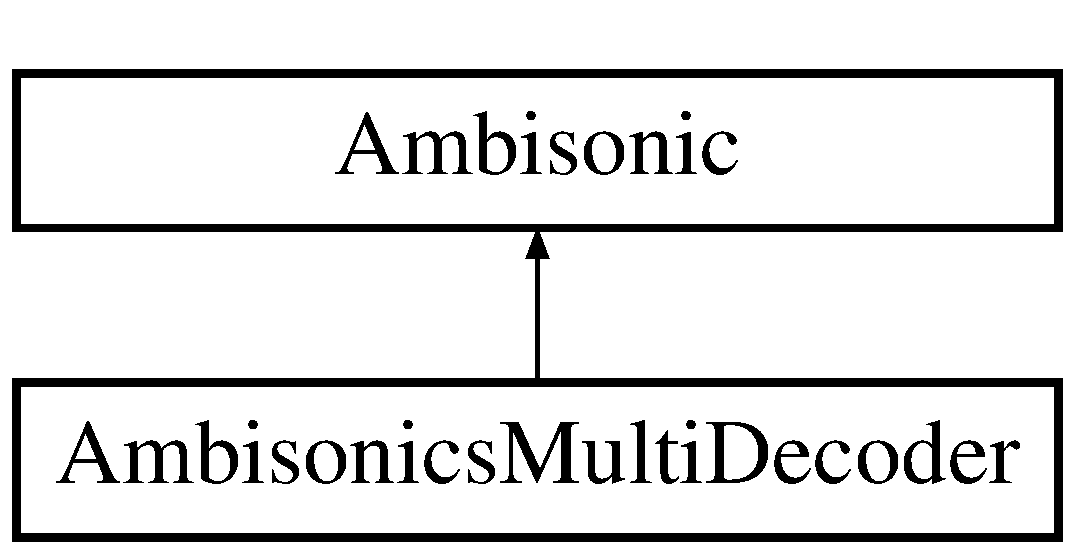
\includegraphics[height=2.000000cm]{class_ambisonics_multi_decoder}
\end{center}
\end{figure}
\subsection*{Public Member Functions}
\begin{DoxyCompactItemize}
\item 
\hyperlink{class_ambisonics_multi_decoder_aa1f1f419fc8b8d032e562009ccb2e6bc}{Ambisonics\-Multi\-Decoder} (long an\-Order=1, long a\-Number\-Of\-Loudspeakers=4, long a\-Mode=Hoa\-\_\-\-Dec\-\_\-\-Ambisonic, long a\-Pinna\-Size=Hoa\-\_\-\-Small, std\-::string a\-Root\-Path=\char`\"{}\char`\"{}, long a\-Vector\-Size=0, long a\-Sampling\-Rate=44100)
\end{DoxyCompactItemize}


\subsection{Detailed Description}


Definition at line 39 of file Ambisonics\-Multi\-Decoder.\-h.



\subsection{Constructor \& Destructor Documentation}
\hypertarget{class_ambisonics_multi_decoder_aa1f1f419fc8b8d032e562009ccb2e6bc}{\index{Ambisonics\-Multi\-Decoder@{Ambisonics\-Multi\-Decoder}!Ambisonics\-Multi\-Decoder@{Ambisonics\-Multi\-Decoder}}
\index{Ambisonics\-Multi\-Decoder@{Ambisonics\-Multi\-Decoder}!AmbisonicsMultiDecoder@{Ambisonics\-Multi\-Decoder}}
\subsubsection[{Ambisonics\-Multi\-Decoder}]{\setlength{\rightskip}{0pt plus 5cm}Ambisonics\-Multi\-Decoder\-::\-Ambisonics\-Multi\-Decoder (
\begin{DoxyParamCaption}
\item[{long}]{an\-Order = {\ttfamily 1}, }
\item[{long}]{a\-Number\-Of\-Loudspeakers = {\ttfamily 4}, }
\item[{long}]{a\-Mode = {\ttfamily Hoa\-\_\-Dec\-\_\-Ambisonic}, }
\item[{long}]{a\-Pinnae\-Size = {\ttfamily Hoa\-\_\-Small}, }
\item[{std\-::string}]{a\-Root\-Path = {\ttfamily \char`\"{}\char`\"{}}, }
\item[{long}]{a\-Vector\-Size = {\ttfamily 0}, }
\item[{long}]{a\-Sampling\-Rate = {\ttfamily 44100}}
\end{DoxyParamCaption}
)}}\label{class_ambisonics_multi_decoder_aa1f1f419fc8b8d032e562009ccb2e6bc}
Hoa\-Library \-: A High Order Ambisonics Library Copyright (c) 2012-\/2013 Julien Colafrancesco, Pierre Guillot, Eliott Paris, C\-I\-C\-M, Universite Paris-\/8. All rights reserved.

Website \-: \href{http://www.mshparisnord.fr/hoalibrary/}{\tt http\-://www.\-mshparisnord.\-fr/hoalibrary/} Contacts \-: \href{mailto:cicm.mshparisnord@gmail.com}{\tt cicm.\-mshparisnord@gmail.\-com}

Redistribution and use in source and binary forms, with or without modification, are permitted provided that the following conditions are met\-:


\begin{DoxyItemize}
\item Redistributions may not be sold, nor may they be used in a commercial product or activity.
\item Redistributions of source code must retain the above copyright notice, this list of conditions and the following disclaimer.
\item Redistributions in binary form must reproduce the above copyright notice, this list of conditions and the following disclaimer in the documentation and/or other materials provided with the distribution.
\item Neither the name of the C\-I\-C\-M nor the names of its contributors may be used to endorse or promote products derived from this software without specific prior written permission.
\end{DoxyItemize}

T\-H\-I\-S S\-O\-F\-T\-W\-A\-R\-E I\-S P\-R\-O\-V\-I\-D\-E\-D B\-Y T\-H\-E C\-O\-P\-Y\-R\-I\-G\-H\-T H\-O\-L\-D\-E\-R\-S A\-N\-D C\-O\-N\-T\-R\-I\-B\-U\-T\-O\-R\-S \char`\"{}\-A\-S I\-S\char`\"{} A\-N\-D A\-N\-Y E\-X\-P\-R\-E\-S\-S O\-R I\-M\-P\-L\-I\-E\-D W\-A\-R\-R\-A\-N\-T\-I\-E\-S, I\-N\-C\-L\-U\-D\-I\-N\-G, B\-U\-T N\-O\-T L\-I\-M\-I\-T\-E\-D T\-O, T\-H\-E I\-M\-P\-L\-I\-E\-D W\-A\-R\-R\-A\-N\-T\-I\-E\-S O\-F M\-E\-R\-C\-H\-A\-N\-T\-A\-B\-I\-L\-I\-T\-Y A\-N\-D F\-I\-T\-N\-E\-S\-S F\-O\-R A P\-A\-R\-T\-I\-C\-U\-L\-A\-R P\-U\-R\-P\-O\-S\-E A\-R\-E D\-I\-S\-C\-L\-A\-I\-M\-E\-D. I\-N N\-O E\-V\-E\-N\-T S\-H\-A\-L\-L T\-H\-E C\-O\-P\-Y\-R\-I\-G\-H\-T H\-O\-L\-D\-E\-R O\-R C\-O\-N\-T\-R\-I\-B\-U\-T\-O\-R\-S B\-E L\-I\-A\-B\-L\-E F\-O\-R A\-N\-Y D\-I\-R\-E\-C\-T, I\-N\-D\-I\-R\-E\-C\-T, I\-N\-C\-I\-D\-E\-N\-T\-A\-L, S\-P\-E\-C\-I\-A\-L, E\-X\-E\-M\-P\-L\-A\-R\-Y, O\-R C\-O\-N\-S\-E\-Q\-U\-E\-N\-T\-I\-A\-L D\-A\-M\-A\-G\-E\-S (I\-N\-C\-L\-U\-D\-I\-N\-G, B\-U\-T N\-O\-T L\-I\-M\-I\-T\-E\-D T\-O, P\-R\-O\-C\-U\-R\-E\-M\-E\-N\-T O\-F S\-U\-B\-S\-T\-I\-T\-U\-T\-E G\-O\-O\-D\-S O\-R S\-E\-R\-V\-I\-C\-E\-S; L\-O\-S\-S O\-F U\-S\-E, D\-A\-T\-A, O\-R P\-R\-O\-F\-I\-T\-S; O\-R B\-U\-S\-I\-N\-E\-S\-S I\-N\-T\-E\-R\-R\-U\-P\-T\-I\-O\-N) H\-O\-W\-E\-V\-E\-R C\-A\-U\-S\-E\-D A\-N\-D O\-N A\-N\-Y T\-H\-E\-O\-R\-Y O\-F L\-I\-A\-B\-I\-L\-I\-T\-Y, W\-H\-E\-T\-H\-E\-R I\-N C\-O\-N\-T\-R\-A\-C\-T, S\-T\-R\-I\-C\-T L\-I\-A\-B\-I\-L\-I\-T\-Y, O\-R T\-O\-R\-T (I\-N\-C\-L\-U\-D\-I\-N\-G N\-E\-G\-L\-I\-G\-E\-N\-C\-E O\-R O\-T\-H\-E\-R\-W\-I\-S\-E) A\-R\-I\-S\-I\-N\-G I\-N A\-N\-Y W\-A\-Y O\-U\-T O\-F T\-H\-E U\-S\-E O\-F T\-H\-I\-S S\-O\-F\-T\-W\-A\-R\-E, E\-V\-E\-N I\-F A\-D\-V\-I\-S\-E\-D O\-F T\-H\-E P\-O\-S\-S\-I\-B\-I\-L\-I\-T\-Y O\-F S\-U\-C\-H D\-A\-M\-A\-G\-E. 

Definition at line 28 of file Ambisonics\-Multi\-Decoder.\-cpp.



The documentation for this class was generated from the following files\-:\begin{DoxyCompactItemize}
\item 
/\-Users/\-Pierre/\-Source\-Tree/\-Hoa\-Library/\-Sources/hoa\-Multi\-Decoder/Ambisonics\-Multi\-Decoder.\-h\item 
/\-Users/\-Pierre/\-Source\-Tree/\-Hoa\-Library/\-Sources/hoa\-Multi\-Decoder/Ambisonics\-Multi\-Decoder.\-cpp\end{DoxyCompactItemize}

\hypertarget{class_ambisonic_spectrum}{\section{Ambisonic\-Spectrum Class Reference}
\label{class_ambisonic_spectrum}\index{Ambisonic\-Spectrum@{Ambisonic\-Spectrum}}
}


{\ttfamily \#include $<$Ambisonic\-Spectrum.\-h$>$}

Inheritance diagram for Ambisonic\-Spectrum\-:\begin{figure}[H]
\begin{center}
\leavevmode
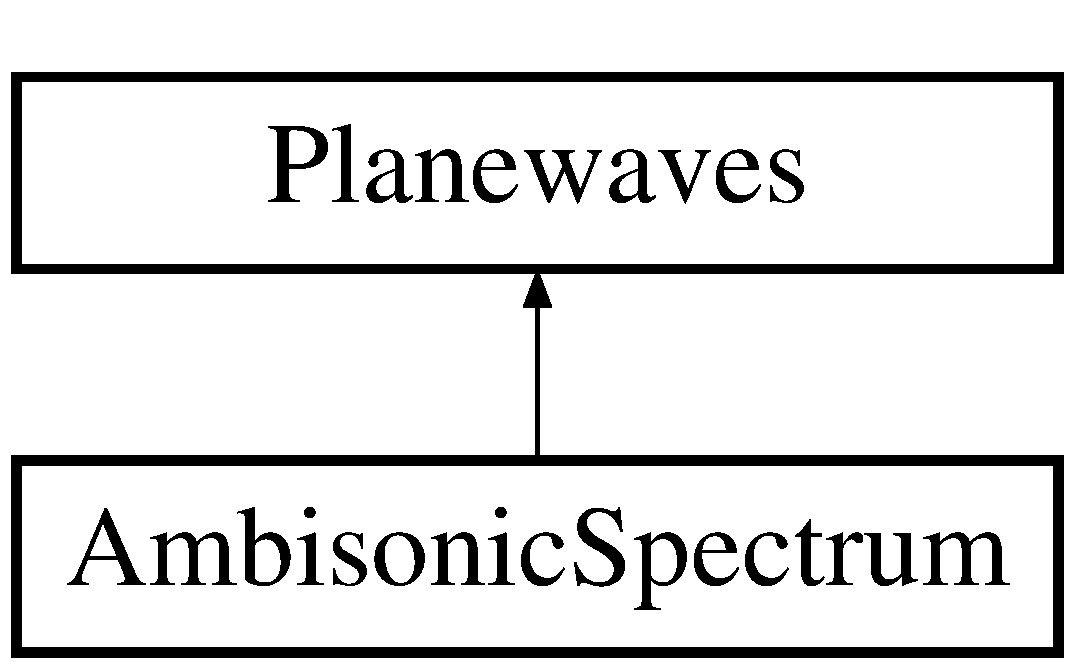
\includegraphics[height=2.000000cm]{class_ambisonic_spectrum}
\end{center}
\end{figure}
\subsection*{Public Member Functions}
\begin{DoxyCompactItemize}
\item 
\hyperlink{class_ambisonic_spectrum_a657f2c97aaab215e95c41f4d07dc8f45}{Ambisonic\-Spectrum} (long a\-Number\-Of\-Loudspeakers=1, long a\-Number\-Of\-Bands=3, long a\-Vector\-Size=0, long a\-Sampling\-Rate=44100)
\item 
\hypertarget{class_ambisonic_spectrum_a67322d6da539d8804711830108289890}{void {\bfseries set\-Number\-Of\-Loudspeakers} (long a\-Number\-Of\-Loudspeakers, bool standard\-On\-Off=0)}\label{class_ambisonic_spectrum_a67322d6da539d8804711830108289890}

\item 
\hypertarget{class_ambisonic_spectrum_a35509a66a23a341cb3fe8db5509cd60c}{void {\bfseries set\-Loudspeaker\-Angle} (long an\-Index, double an\-Angle)}\label{class_ambisonic_spectrum_a35509a66a23a341cb3fe8db5509cd60c}

\item 
\hypertarget{class_ambisonic_spectrum_ae50e8aebafb67fc1883b1b4343c69018}{void {\bfseries set\-Frequency\-Band} (long an\-Index, double a\-Frequency)}\label{class_ambisonic_spectrum_ae50e8aebafb67fc1883b1b4343c69018}

\item 
\hypertarget{class_ambisonic_spectrum_a21fb69a71c815e1ab5bf350668b5dc0c}{void {\bfseries set\-Number\-Of\-Bands} (long a\-Number\-Of\-Bands)}\label{class_ambisonic_spectrum_a21fb69a71c815e1ab5bf350668b5dc0c}

\item 
\hypertarget{class_ambisonic_spectrum_abde7474b423c03a64a4f810dac2805c6}{double {\bfseries get\-Amplitude} (long a\-Band\-Index)}\label{class_ambisonic_spectrum_abde7474b423c03a64a4f810dac2805c6}

\item 
\hypertarget{class_ambisonic_spectrum_a2c98b11e9e41def8f7d6e24ef34a144c}{double {\bfseries get\-Abscissa} (long a\-Band\-Index)}\label{class_ambisonic_spectrum_a2c98b11e9e41def8f7d6e24ef34a144c}

\item 
\hypertarget{class_ambisonic_spectrum_a7d91f3340282b610dca8f5d6133029f5}{double {\bfseries get\-Ordinate} (long a\-Band\-Index)}\label{class_ambisonic_spectrum_a7d91f3340282b610dca8f5d6133029f5}

\item 
\hypertarget{class_ambisonic_spectrum_a05b2917412c783f96af3300c6b93a615}{double {\bfseries get\-Radius} (long a\-Band\-Index)}\label{class_ambisonic_spectrum_a05b2917412c783f96af3300c6b93a615}

\item 
\hypertarget{class_ambisonic_spectrum_a5db3862c241c1803091a180f95151b4d}{double {\bfseries get\-Angle} (long a\-Band\-Index)}\label{class_ambisonic_spectrum_a5db3862c241c1803091a180f95151b4d}

\item 
\hypertarget{class_ambisonic_spectrum_a6c4d7db26791c55b063cb6e096c199c0}{double {\bfseries get\-Log\-Amplitude} (long a\-Band\-Index)}\label{class_ambisonic_spectrum_a6c4d7db26791c55b063cb6e096c199c0}

\item 
\hypertarget{class_ambisonic_spectrum_a5a0194caed12270647a345052c17ca14}{double {\bfseries get\-Log\-Abscissa} (long a\-Band\-Index)}\label{class_ambisonic_spectrum_a5a0194caed12270647a345052c17ca14}

\item 
\hypertarget{class_ambisonic_spectrum_a8e63b1e2663ee142ff51c31b57028ba2}{double {\bfseries get\-Log\-Ordinate} (long a\-Band\-Index)}\label{class_ambisonic_spectrum_a8e63b1e2663ee142ff51c31b57028ba2}

\item 
\hypertarget{class_ambisonic_spectrum_a24d7d8d26f1f5257fe684babc648f6c6}{double {\bfseries get\-Log\-Radius} (long a\-Band\-Index)}\label{class_ambisonic_spectrum_a24d7d8d26f1f5257fe684babc648f6c6}

\item 
\hypertarget{class_ambisonic_spectrum_a65e453f0de97f94d09dd5af107b711e2}{double {\bfseries get\-Log\-Angle} (long a\-Band\-Index)}\label{class_ambisonic_spectrum_a65e453f0de97f94d09dd5af107b711e2}

\item 
\hypertarget{class_ambisonic_spectrum_a85d13a81ce2d971465a0715e9889126f}{double {\bfseries get\-Frequency\-Band} (long an\-Index)}\label{class_ambisonic_spectrum_a85d13a81ce2d971465a0715e9889126f}

\item 
\hypertarget{class_ambisonic_spectrum_a0982fde433c0a1f2d0cbb22340e0c756}{long {\bfseries get\-Number\-Of\-Bands} ()}\label{class_ambisonic_spectrum_a0982fde433c0a1f2d0cbb22340e0c756}

\item 
\hypertarget{class_ambisonic_spectrum_a83e25eaf71ec3cd3c37b0f74af778dcd}{void {\bfseries set\-Vector\-Size} (long a\-Vector\-Size)}\label{class_ambisonic_spectrum_a83e25eaf71ec3cd3c37b0f74af778dcd}

\item 
\hypertarget{class_ambisonic_spectrum_a7bd00bbe40241407a84ea6dc8c5df1bd}{void {\bfseries set\-Sampling\-Rate} (long a\-Sampling\-Rate)}\label{class_ambisonic_spectrum_a7bd00bbe40241407a84ea6dc8c5df1bd}

\item 
\hypertarget{class_ambisonic_spectrum_aec69f768c208a83f5ce55268b942ca1a}{void {\bfseries process} (const double $\ast$const $\ast$inputs)}\label{class_ambisonic_spectrum_aec69f768c208a83f5ce55268b942ca1a}

\item 
\hypertarget{class_ambisonic_spectrum_ab3ab5df934defcaa6e86502f61589b21}{void {\bfseries tick} ()}\label{class_ambisonic_spectrum_ab3ab5df934defcaa6e86502f61589b21}

\end{DoxyCompactItemize}
\subsection*{Additional Inherited Members}


\subsection{Detailed Description}
Hoa\-Library \-: A High Order Ambisonics Library Copyright (c) 2012-\/2013 Julien Colafrancesco, Pierre Guillot, Eliott Paris, C\-I\-C\-M, Universite Paris-\/8. All rights reserved.\-re Guillot, C\-I\-C\-M -\/ Université Paris 8 All rights reserved.

Website \-: \href{http://www.mshparisnord.fr/HoaLibrary/}{\tt http\-://www.\-mshparisnord.\-fr/\-Hoa\-Library/} Contacts \-: \href{mailto:cicm.mshparisnord@gmail.com}{\tt cicm.\-mshparisnord@gmail.\-com}

This file is part of H\-O\-A L\-I\-B\-R\-A\-R\-Y.

H\-O\-A L\-I\-B\-R\-A\-R\-Y is free software\-: you can redistribute it and/or modify it under the terms of the G\-N\-U General Public License as published by the Free Software Foundation, either version 3 of the License, or (at your option) any later version.

This program is distributed in the hope that it will be useful, but W\-I\-T\-H\-O\-U\-T A\-N\-Y W\-A\-R\-R\-A\-N\-T\-Y; without even the implied warranty of M\-E\-R\-C\-H\-A\-N\-T\-A\-B\-I\-L\-I\-T\-Y or F\-I\-T\-N\-E\-S\-S F\-O\-R A P\-A\-R\-T\-I\-C\-U\-L\-A\-R P\-U\-R\-P\-O\-S\-E. See the G\-N\-U General Public License for more details.

You should have received a copy of the G\-N\-U General Public License along with this program. If not, see \href{http://www.gnu.org/licenses/}{\tt http\-://www.\-gnu.\-org/licenses/}. 

\subsection{Constructor \& Destructor Documentation}
\hypertarget{class_ambisonic_spectrum_a657f2c97aaab215e95c41f4d07dc8f45}{\index{Ambisonic\-Spectrum@{Ambisonic\-Spectrum}!Ambisonic\-Spectrum@{Ambisonic\-Spectrum}}
\index{Ambisonic\-Spectrum@{Ambisonic\-Spectrum}!AmbisonicSpectrum@{Ambisonic\-Spectrum}}
\subsubsection[{Ambisonic\-Spectrum}]{\setlength{\rightskip}{0pt plus 5cm}Ambisonic\-Spectrum\-::\-Ambisonic\-Spectrum (
\begin{DoxyParamCaption}
\item[{long}]{a\-Number\-Of\-Loudspeakers = {\ttfamily 1}, }
\item[{long}]{a\-Number\-Of\-Bands = {\ttfamily 3}, }
\item[{long}]{a\-Vector\-Size = {\ttfamily 0}, }
\item[{long}]{a\-Sampling\-Rate = {\ttfamily 44100}}
\end{DoxyParamCaption}
)}}\label{class_ambisonic_spectrum_a657f2c97aaab215e95c41f4d07dc8f45}
Hoa\-Library \-: A High Order Ambisonics Library Copyright (c) 2012-\/2013 Julien Colafrancesco, Pierre Guillot, Eliott Paris, C\-I\-C\-M, Universite Paris-\/8. All rights reserved.\-re Guillot, C\-I\-C\-M -\/ Université Paris 8 All rights reserved.

Website \-: \href{http://www.mshparisnord.fr/HoaLibrary/}{\tt http\-://www.\-mshparisnord.\-fr/\-Hoa\-Library/} Contacts \-: \href{mailto:cicm.mshparisnord@gmail.com}{\tt cicm.\-mshparisnord@gmail.\-com}

This file is part of H\-O\-A L\-I\-B\-R\-A\-R\-Y.

H\-O\-A L\-I\-B\-R\-A\-R\-Y is free software\-: you can redistribute it and/or modify it under the terms of the G\-N\-U General Public License as published by the Free Software Foundation, either version 3 of the License, or (at your option) any later version.

This program is distributed in the hope that it will be useful, but W\-I\-T\-H\-O\-U\-T A\-N\-Y W\-A\-R\-R\-A\-N\-T\-Y; without even the implied warranty of M\-E\-R\-C\-H\-A\-N\-T\-A\-B\-I\-L\-I\-T\-Y or F\-I\-T\-N\-E\-S\-S F\-O\-R A P\-A\-R\-T\-I\-C\-U\-L\-A\-R P\-U\-R\-P\-O\-S\-E. See the G\-N\-U General Public License for more details.

You should have received a copy of the G\-N\-U General Public License along with this program. If not, see \href{http://www.gnu.org/licenses/}{\tt http\-://www.\-gnu.\-org/licenses/}. 

The documentation for this class was generated from the following files\-:\begin{DoxyCompactItemize}
\item 
/\-Users/\-Pierre/\-Source\-Tree/\-Hoa\-Library/\-Sources/hoa\-Spectrum/Ambisonic\-Spectrum.\-h\item 
/\-Users/\-Pierre/\-Source\-Tree/\-Hoa\-Library/\-Sources/hoa\-Spectrum/Ambisonic\-Spectrum.\-cpp\end{DoxyCompactItemize}

\hypertarget{class_ambisonics_restitution}{\section{Ambisonics\-Restitution Class Reference}
\label{class_ambisonics_restitution}\index{Ambisonics\-Restitution@{Ambisonics\-Restitution}}
}
Inheritance diagram for Ambisonics\-Restitution\-:\begin{figure}[H]
\begin{center}
\leavevmode
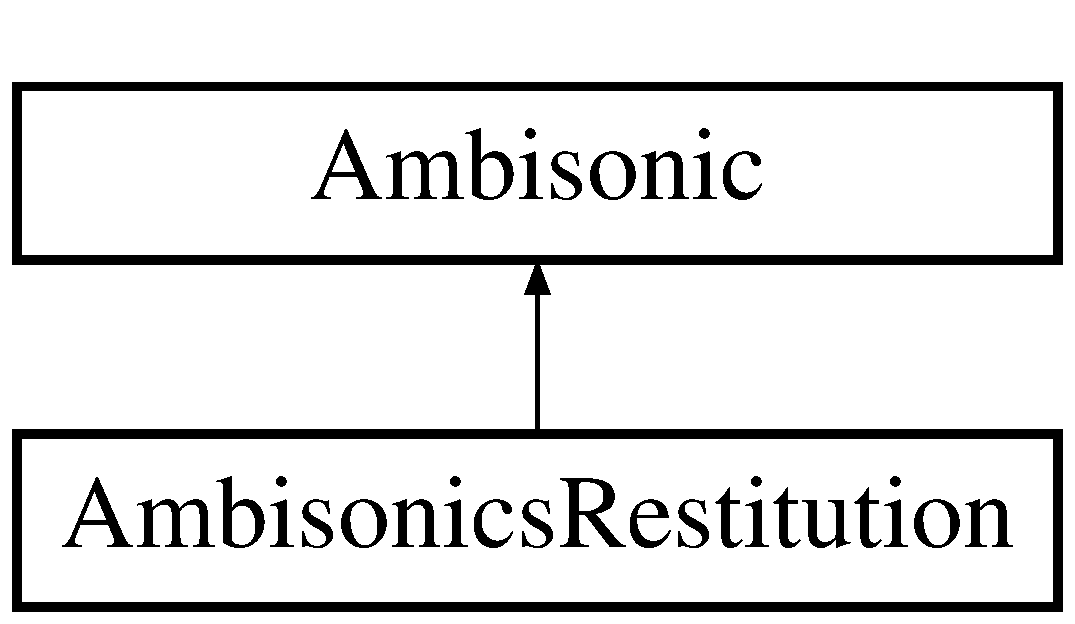
\includegraphics[height=2.000000cm]{class_ambisonics_restitution}
\end{center}
\end{figure}
\subsection*{Public Member Functions}
\begin{DoxyCompactItemize}
\item 
\hyperlink{class_ambisonics_restitution_a287ce5a5b5d247af6c11e7bd0e50a4ab}{Ambisonics\-Restitution} (long an\-Order=1, long a\-Number\-Of\-Loudspeakers=5, long a\-Resitution\-Mode=Hoa\-\_\-\-Amplitude\-\_\-\-Panning, long a\-Vector\-Size=0)
\end{DoxyCompactItemize}


\subsection{Detailed Description}


Definition at line 37 of file Ambisonics\-Restitution.\-h.



\subsection{Constructor \& Destructor Documentation}
\hypertarget{class_ambisonics_restitution_a287ce5a5b5d247af6c11e7bd0e50a4ab}{\index{Ambisonics\-Restitution@{Ambisonics\-Restitution}!Ambisonics\-Restitution@{Ambisonics\-Restitution}}
\index{Ambisonics\-Restitution@{Ambisonics\-Restitution}!AmbisonicsRestitution@{Ambisonics\-Restitution}}
\subsubsection[{Ambisonics\-Restitution}]{\setlength{\rightskip}{0pt plus 5cm}Ambisonics\-Restitution\-::\-Ambisonics\-Restitution (
\begin{DoxyParamCaption}
\item[{long}]{an\-Order = {\ttfamily 1}, }
\item[{long}]{a\-Number\-Of\-Loudspeakers = {\ttfamily 5}, }
\item[{long}]{a\-Resitution\-Mode = {\ttfamily Hoa\-\_\-Amplitude\-\_\-Panning}, }
\item[{long}]{a\-Vector\-Size = {\ttfamily 0}}
\end{DoxyParamCaption}
)}}\label{class_ambisonics_restitution_a287ce5a5b5d247af6c11e7bd0e50a4ab}
Hoa\-Library \-: A High Order Ambisonics Library Copyright (c) 2012-\/2013 Julien Colafrancesco, Pierre Guillot, Eliott Paris, C\-I\-C\-M, Universite Paris-\/8. All rights reserved.

Website \-: \href{http://www.mshparisnord.fr/hoalibrary/}{\tt http\-://www.\-mshparisnord.\-fr/hoalibrary/} Contacts \-: \href{mailto:cicm.mshparisnord@gmail.com}{\tt cicm.\-mshparisnord@gmail.\-com}

Redistribution and use in source and binary forms, with or without modification, are permitted provided that the following conditions are met\-:


\begin{DoxyItemize}
\item Redistributions may not be sold, nor may they be used in a commercial product or activity.
\item Redistributions of source code must retain the above copyright notice, this list of conditions and the following disclaimer.
\item Redistributions in binary form must reproduce the above copyright notice, this list of conditions and the following disclaimer in the documentation and/or other materials provided with the distribution.
\item Neither the name of the C\-I\-C\-M nor the names of its contributors may be used to endorse or promote products derived from this software without specific prior written permission.
\end{DoxyItemize}

T\-H\-I\-S S\-O\-F\-T\-W\-A\-R\-E I\-S P\-R\-O\-V\-I\-D\-E\-D B\-Y T\-H\-E C\-O\-P\-Y\-R\-I\-G\-H\-T H\-O\-L\-D\-E\-R\-S A\-N\-D C\-O\-N\-T\-R\-I\-B\-U\-T\-O\-R\-S \char`\"{}\-A\-S I\-S\char`\"{} A\-N\-D A\-N\-Y E\-X\-P\-R\-E\-S\-S O\-R I\-M\-P\-L\-I\-E\-D W\-A\-R\-R\-A\-N\-T\-I\-E\-S, I\-N\-C\-L\-U\-D\-I\-N\-G, B\-U\-T N\-O\-T L\-I\-M\-I\-T\-E\-D T\-O, T\-H\-E I\-M\-P\-L\-I\-E\-D W\-A\-R\-R\-A\-N\-T\-I\-E\-S O\-F M\-E\-R\-C\-H\-A\-N\-T\-A\-B\-I\-L\-I\-T\-Y A\-N\-D F\-I\-T\-N\-E\-S\-S F\-O\-R A P\-A\-R\-T\-I\-C\-U\-L\-A\-R P\-U\-R\-P\-O\-S\-E A\-R\-E D\-I\-S\-C\-L\-A\-I\-M\-E\-D. I\-N N\-O E\-V\-E\-N\-T S\-H\-A\-L\-L T\-H\-E C\-O\-P\-Y\-R\-I\-G\-H\-T H\-O\-L\-D\-E\-R O\-R C\-O\-N\-T\-R\-I\-B\-U\-T\-O\-R\-S B\-E L\-I\-A\-B\-L\-E F\-O\-R A\-N\-Y D\-I\-R\-E\-C\-T, I\-N\-D\-I\-R\-E\-C\-T, I\-N\-C\-I\-D\-E\-N\-T\-A\-L, S\-P\-E\-C\-I\-A\-L, E\-X\-E\-M\-P\-L\-A\-R\-Y, O\-R C\-O\-N\-S\-E\-Q\-U\-E\-N\-T\-I\-A\-L D\-A\-M\-A\-G\-E\-S (I\-N\-C\-L\-U\-D\-I\-N\-G, B\-U\-T N\-O\-T L\-I\-M\-I\-T\-E\-D T\-O, P\-R\-O\-C\-U\-R\-E\-M\-E\-N\-T O\-F S\-U\-B\-S\-T\-I\-T\-U\-T\-E G\-O\-O\-D\-S O\-R S\-E\-R\-V\-I\-C\-E\-S; L\-O\-S\-S O\-F U\-S\-E, D\-A\-T\-A, O\-R P\-R\-O\-F\-I\-T\-S; O\-R B\-U\-S\-I\-N\-E\-S\-S I\-N\-T\-E\-R\-R\-U\-P\-T\-I\-O\-N) H\-O\-W\-E\-V\-E\-R C\-A\-U\-S\-E\-D A\-N\-D O\-N A\-N\-Y T\-H\-E\-O\-R\-Y O\-F L\-I\-A\-B\-I\-L\-I\-T\-Y, W\-H\-E\-T\-H\-E\-R I\-N C\-O\-N\-T\-R\-A\-C\-T, S\-T\-R\-I\-C\-T L\-I\-A\-B\-I\-L\-I\-T\-Y, O\-R T\-O\-R\-T (I\-N\-C\-L\-U\-D\-I\-N\-G N\-E\-G\-L\-I\-G\-E\-N\-C\-E O\-R O\-T\-H\-E\-R\-W\-I\-S\-E) A\-R\-I\-S\-I\-N\-G I\-N A\-N\-Y W\-A\-Y O\-U\-T O\-F T\-H\-E U\-S\-E O\-F T\-H\-I\-S S\-O\-F\-T\-W\-A\-R\-E, E\-V\-E\-N I\-F A\-D\-V\-I\-S\-E\-D O\-F T\-H\-E P\-O\-S\-S\-I\-B\-I\-L\-I\-T\-Y O\-F S\-U\-C\-H D\-A\-M\-A\-G\-E. 

Definition at line 28 of file Ambisonics\-Restitution.\-cpp.



The documentation for this class was generated from the following files\-:\begin{DoxyCompactItemize}
\item 
/\-Users/elioton/\-Documents/programmation/\-C\-I\-C\-M/source\-Tree/\-Hoa\-Library/\-Sources/hoa\-Restitution/Ambisonics\-Restitution.\-h\item 
/\-Users/elioton/\-Documents/programmation/\-C\-I\-C\-M/source\-Tree/\-Hoa\-Library/\-Sources/hoa\-Restitution/Ambisonics\-Restitution.\-cpp\end{DoxyCompactItemize}

\hypertarget{class_ambisonics_scope}{\section{Ambisonics\-Scope Class Reference}
\label{class_ambisonics_scope}\index{Ambisonics\-Scope@{Ambisonics\-Scope}}
}


{\ttfamily \#include $<$Ambisonics\-Scope.\-h$>$}

Inheritance diagram for Ambisonics\-Scope\-:\begin{figure}[H]
\begin{center}
\leavevmode
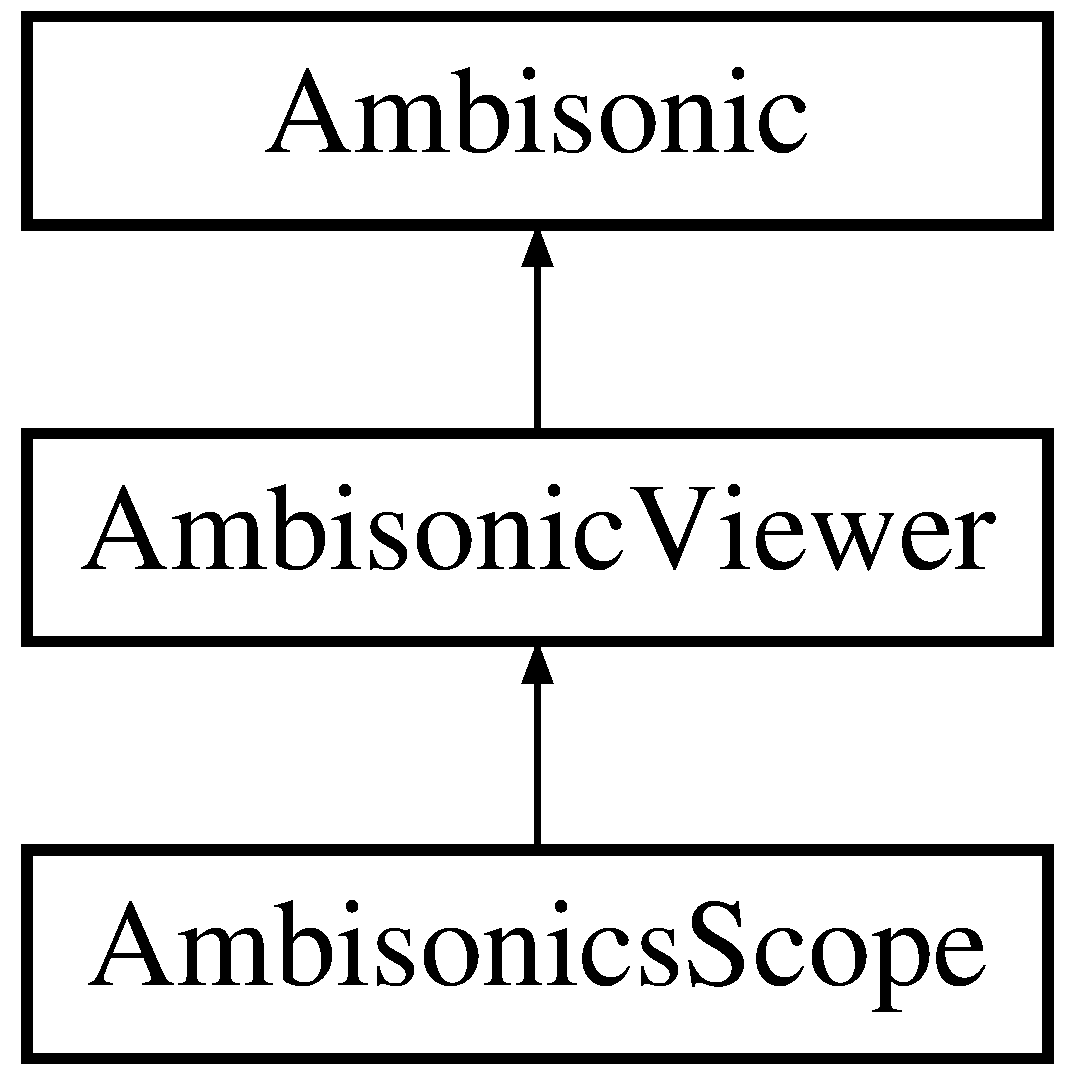
\includegraphics[height=2.000000cm]{class_ambisonics_scope}
\end{center}
\end{figure}
\subsection*{Public Member Functions}
\begin{DoxyCompactItemize}
\item 
\hyperlink{class_ambisonics_scope_a0b7854d037fb52d23898f390abc3a50c}{Ambisonics\-Scope} (long an\-Order=1, long a\-Vector\-Size=0, long a\-Sampling\-Rate=44100.)
\end{DoxyCompactItemize}


\subsection{Detailed Description}
Hoa\-Library \-: A High Order Ambisonics Library Copyright (c) 2012-\/2013 Julien Colafrancesco, Pierre Guillot, Eliott Paris, C\-I\-C\-M, Universite Paris-\/8. All rights reserved.

Website \-: \href{http://www.mshparisnord.fr/hoalibrary/}{\tt http\-://www.\-mshparisnord.\-fr/hoalibrary/} Contacts \-: \href{mailto:cicm.mshparisnord@gmail.com}{\tt cicm.\-mshparisnord@gmail.\-com}

Redistribution and use in source and binary forms, with or without modification, are permitted provided that the following conditions are met\-:


\begin{DoxyItemize}
\item Redistributions may not be sold, nor may they be used in a commercial product or activity.
\item Redistributions of source code must retain the above copyright notice, this list of conditions and the following disclaimer.
\item Redistributions in binary form must reproduce the above copyright notice, this list of conditions and the following disclaimer in the documentation and/or other materials provided with the distribution.
\item Neither the name of the C\-I\-C\-M nor the names of its contributors may be used to endorse or promote products derived from this software without specific prior written permission.
\end{DoxyItemize}

T\-H\-I\-S S\-O\-F\-T\-W\-A\-R\-E I\-S P\-R\-O\-V\-I\-D\-E\-D B\-Y T\-H\-E C\-O\-P\-Y\-R\-I\-G\-H\-T H\-O\-L\-D\-E\-R\-S A\-N\-D C\-O\-N\-T\-R\-I\-B\-U\-T\-O\-R\-S \char`\"{}\-A\-S I\-S\char`\"{} A\-N\-D A\-N\-Y E\-X\-P\-R\-E\-S\-S O\-R I\-M\-P\-L\-I\-E\-D W\-A\-R\-R\-A\-N\-T\-I\-E\-S, I\-N\-C\-L\-U\-D\-I\-N\-G, B\-U\-T N\-O\-T L\-I\-M\-I\-T\-E\-D T\-O, T\-H\-E I\-M\-P\-L\-I\-E\-D W\-A\-R\-R\-A\-N\-T\-I\-E\-S O\-F M\-E\-R\-C\-H\-A\-N\-T\-A\-B\-I\-L\-I\-T\-Y A\-N\-D F\-I\-T\-N\-E\-S\-S F\-O\-R A P\-A\-R\-T\-I\-C\-U\-L\-A\-R P\-U\-R\-P\-O\-S\-E A\-R\-E D\-I\-S\-C\-L\-A\-I\-M\-E\-D. I\-N N\-O E\-V\-E\-N\-T S\-H\-A\-L\-L T\-H\-E C\-O\-P\-Y\-R\-I\-G\-H\-T H\-O\-L\-D\-E\-R O\-R C\-O\-N\-T\-R\-I\-B\-U\-T\-O\-R\-S B\-E L\-I\-A\-B\-L\-E F\-O\-R A\-N\-Y D\-I\-R\-E\-C\-T, I\-N\-D\-I\-R\-E\-C\-T, I\-N\-C\-I\-D\-E\-N\-T\-A\-L, S\-P\-E\-C\-I\-A\-L, E\-X\-E\-M\-P\-L\-A\-R\-Y, O\-R C\-O\-N\-S\-E\-Q\-U\-E\-N\-T\-I\-A\-L D\-A\-M\-A\-G\-E\-S (I\-N\-C\-L\-U\-D\-I\-N\-G, B\-U\-T N\-O\-T L\-I\-M\-I\-T\-E\-D T\-O, P\-R\-O\-C\-U\-R\-E\-M\-E\-N\-T O\-F S\-U\-B\-S\-T\-I\-T\-U\-T\-E G\-O\-O\-D\-S O\-R S\-E\-R\-V\-I\-C\-E\-S; L\-O\-S\-S O\-F U\-S\-E, D\-A\-T\-A, O\-R P\-R\-O\-F\-I\-T\-S; O\-R B\-U\-S\-I\-N\-E\-S\-S I\-N\-T\-E\-R\-R\-U\-P\-T\-I\-O\-N) H\-O\-W\-E\-V\-E\-R C\-A\-U\-S\-E\-D A\-N\-D O\-N A\-N\-Y T\-H\-E\-O\-R\-Y O\-F L\-I\-A\-B\-I\-L\-I\-T\-Y, W\-H\-E\-T\-H\-E\-R I\-N C\-O\-N\-T\-R\-A\-C\-T, S\-T\-R\-I\-C\-T L\-I\-A\-B\-I\-L\-I\-T\-Y, O\-R T\-O\-R\-T (I\-N\-C\-L\-U\-D\-I\-N\-G N\-E\-G\-L\-I\-G\-E\-N\-C\-E O\-R O\-T\-H\-E\-R\-W\-I\-S\-E) A\-R\-I\-S\-I\-N\-G I\-N A\-N\-Y W\-A\-Y O\-U\-T O\-F T\-H\-E U\-S\-E O\-F T\-H\-I\-S S\-O\-F\-T\-W\-A\-R\-E, E\-V\-E\-N I\-F A\-D\-V\-I\-S\-E\-D O\-F T\-H\-E P\-O\-S\-S\-I\-B\-I\-L\-I\-T\-Y O\-F S\-U\-C\-H D\-A\-M\-A\-G\-E. 

Definition at line 31 of file Ambisonics\-Scope.\-h.



\subsection{Constructor \& Destructor Documentation}
\hypertarget{class_ambisonics_scope_a0b7854d037fb52d23898f390abc3a50c}{\index{Ambisonics\-Scope@{Ambisonics\-Scope}!Ambisonics\-Scope@{Ambisonics\-Scope}}
\index{Ambisonics\-Scope@{Ambisonics\-Scope}!AmbisonicsScope@{Ambisonics\-Scope}}
\subsubsection[{Ambisonics\-Scope}]{\setlength{\rightskip}{0pt plus 5cm}Ambisonics\-Scope\-::\-Ambisonics\-Scope (
\begin{DoxyParamCaption}
\item[{long}]{an\-Order = {\ttfamily 1}, }
\item[{long}]{a\-Vector\-Size = {\ttfamily 0}, }
\item[{long}]{a\-Sampling\-Rate = {\ttfamily 44100.}}
\end{DoxyParamCaption}
)}}\label{class_ambisonics_scope_a0b7854d037fb52d23898f390abc3a50c}
Hoa\-Library \-: A High Order Ambisonics Library Copyright (c) 2012-\/2013 Julien Colafrancesco, Pierre Guillot, Eliott Paris, C\-I\-C\-M, Universite Paris-\/8. All rights reserved.

Website \-: \href{http://www.mshparisnord.fr/hoalibrary/}{\tt http\-://www.\-mshparisnord.\-fr/hoalibrary/} Contacts \-: \href{mailto:cicm.mshparisnord@gmail.com}{\tt cicm.\-mshparisnord@gmail.\-com}

Redistribution and use in source and binary forms, with or without modification, are permitted provided that the following conditions are met\-:


\begin{DoxyItemize}
\item Redistributions may not be sold, nor may they be used in a commercial product or activity.
\item Redistributions of source code must retain the above copyright notice, this list of conditions and the following disclaimer.
\item Redistributions in binary form must reproduce the above copyright notice, this list of conditions and the following disclaimer in the documentation and/or other materials provided with the distribution.
\item Neither the name of the C\-I\-C\-M nor the names of its contributors may be used to endorse or promote products derived from this software without specific prior written permission.
\end{DoxyItemize}

T\-H\-I\-S S\-O\-F\-T\-W\-A\-R\-E I\-S P\-R\-O\-V\-I\-D\-E\-D B\-Y T\-H\-E C\-O\-P\-Y\-R\-I\-G\-H\-T H\-O\-L\-D\-E\-R\-S A\-N\-D C\-O\-N\-T\-R\-I\-B\-U\-T\-O\-R\-S \char`\"{}\-A\-S I\-S\char`\"{} A\-N\-D A\-N\-Y E\-X\-P\-R\-E\-S\-S O\-R I\-M\-P\-L\-I\-E\-D W\-A\-R\-R\-A\-N\-T\-I\-E\-S, I\-N\-C\-L\-U\-D\-I\-N\-G, B\-U\-T N\-O\-T L\-I\-M\-I\-T\-E\-D T\-O, T\-H\-E I\-M\-P\-L\-I\-E\-D W\-A\-R\-R\-A\-N\-T\-I\-E\-S O\-F M\-E\-R\-C\-H\-A\-N\-T\-A\-B\-I\-L\-I\-T\-Y A\-N\-D F\-I\-T\-N\-E\-S\-S F\-O\-R A P\-A\-R\-T\-I\-C\-U\-L\-A\-R P\-U\-R\-P\-O\-S\-E A\-R\-E D\-I\-S\-C\-L\-A\-I\-M\-E\-D. I\-N N\-O E\-V\-E\-N\-T S\-H\-A\-L\-L T\-H\-E C\-O\-P\-Y\-R\-I\-G\-H\-T H\-O\-L\-D\-E\-R O\-R C\-O\-N\-T\-R\-I\-B\-U\-T\-O\-R\-S B\-E L\-I\-A\-B\-L\-E F\-O\-R A\-N\-Y D\-I\-R\-E\-C\-T, I\-N\-D\-I\-R\-E\-C\-T, I\-N\-C\-I\-D\-E\-N\-T\-A\-L, S\-P\-E\-C\-I\-A\-L, E\-X\-E\-M\-P\-L\-A\-R\-Y, O\-R C\-O\-N\-S\-E\-Q\-U\-E\-N\-T\-I\-A\-L D\-A\-M\-A\-G\-E\-S (I\-N\-C\-L\-U\-D\-I\-N\-G, B\-U\-T N\-O\-T L\-I\-M\-I\-T\-E\-D T\-O, P\-R\-O\-C\-U\-R\-E\-M\-E\-N\-T O\-F S\-U\-B\-S\-T\-I\-T\-U\-T\-E G\-O\-O\-D\-S O\-R S\-E\-R\-V\-I\-C\-E\-S; L\-O\-S\-S O\-F U\-S\-E, D\-A\-T\-A, O\-R P\-R\-O\-F\-I\-T\-S; O\-R B\-U\-S\-I\-N\-E\-S\-S I\-N\-T\-E\-R\-R\-U\-P\-T\-I\-O\-N) H\-O\-W\-E\-V\-E\-R C\-A\-U\-S\-E\-D A\-N\-D O\-N A\-N\-Y T\-H\-E\-O\-R\-Y O\-F L\-I\-A\-B\-I\-L\-I\-T\-Y, W\-H\-E\-T\-H\-E\-R I\-N C\-O\-N\-T\-R\-A\-C\-T, S\-T\-R\-I\-C\-T L\-I\-A\-B\-I\-L\-I\-T\-Y, O\-R T\-O\-R\-T (I\-N\-C\-L\-U\-D\-I\-N\-G N\-E\-G\-L\-I\-G\-E\-N\-C\-E O\-R O\-T\-H\-E\-R\-W\-I\-S\-E) A\-R\-I\-S\-I\-N\-G I\-N A\-N\-Y W\-A\-Y O\-U\-T O\-F T\-H\-E U\-S\-E O\-F T\-H\-I\-S S\-O\-F\-T\-W\-A\-R\-E, E\-V\-E\-N I\-F A\-D\-V\-I\-S\-E\-D O\-F T\-H\-E P\-O\-S\-S\-I\-B\-I\-L\-I\-T\-Y O\-F S\-U\-C\-H D\-A\-M\-A\-G\-E. 

Definition at line 28 of file Ambisonics\-Scope.\-cpp.



The documentation for this class was generated from the following files\-:\begin{DoxyCompactItemize}
\item 
/\-Users/\-Pierre/\-Source\-Tree/\-Hoa\-Library/\-Sources/hoa\-Scope/Ambisonics\-Scope.\-h\item 
/\-Users/\-Pierre/\-Source\-Tree/\-Hoa\-Library/\-Sources/hoa\-Scope/Ambisonics\-Scope.\-cpp\end{DoxyCompactItemize}

\hypertarget{class_ambisonic_virtual_mic_u_i}{\section{Ambisonic\-Virtual\-Mic\-U\-I Class Reference}
\label{class_ambisonic_virtual_mic_u_i}\index{Ambisonic\-Virtual\-Mic\-U\-I@{Ambisonic\-Virtual\-Mic\-U\-I}}
}


The documentation for this class was generated from the following files\-:\begin{DoxyCompactItemize}
\item 
/\-Users/\-Pierre/\-Source\-Tree/\-Hoa\-Library/\-Sources/hoa\-Recomposer/Ambisonic\-Virtual\-Mic\-U\-I.\-h\item 
/\-Users/\-Pierre/\-Source\-Tree/\-Hoa\-Library/\-Sources/hoa\-Recomposer/Ambisonic\-Virtual\-Mic\-U\-I.\-cpp\end{DoxyCompactItemize}

\hypertarget{class_ambisonic_virtual_mic_u_i_manager}{\section{Ambisonic\-Virtual\-Mic\-U\-I\-Manager Class Reference}
\label{class_ambisonic_virtual_mic_u_i_manager}\index{Ambisonic\-Virtual\-Mic\-U\-I\-Manager@{Ambisonic\-Virtual\-Mic\-U\-I\-Manager}}
}


\subsection{Detailed Description}


Definition at line 32 of file Ambisonic\-Virtual\-Mic\-U\-I\-Manager.\-h.



The documentation for this class was generated from the following files\-:\begin{DoxyCompactItemize}
\item 
/\-Users/\-Pierre/\-Source\-Tree/\-Hoa\-Library/\-Sources/hoa\-Recomposer/Ambisonic\-Virtual\-Mic\-U\-I\-Manager.\-h\item 
/\-Users/\-Pierre/\-Source\-Tree/\-Hoa\-Library/\-Sources/hoa\-Recomposer/Ambisonic\-Virtual\-Mic\-U\-I\-Manager.\-cpp\end{DoxyCompactItemize}

\hypertarget{class_hoa3_d_1_1_decoder}{\section{Hoa3\-D\-:\-:Decoder Class Reference}
\label{class_hoa3_d_1_1_decoder}\index{Hoa3\-D\-::\-Decoder@{Hoa3\-D\-::\-Decoder}}
}


The ambisonic decoder.  




{\ttfamily \#include $<$Decoder.\-h$>$}

Inheritance diagram for Hoa3\-D\-:\-:Decoder\-:\begin{figure}[H]
\begin{center}
\leavevmode
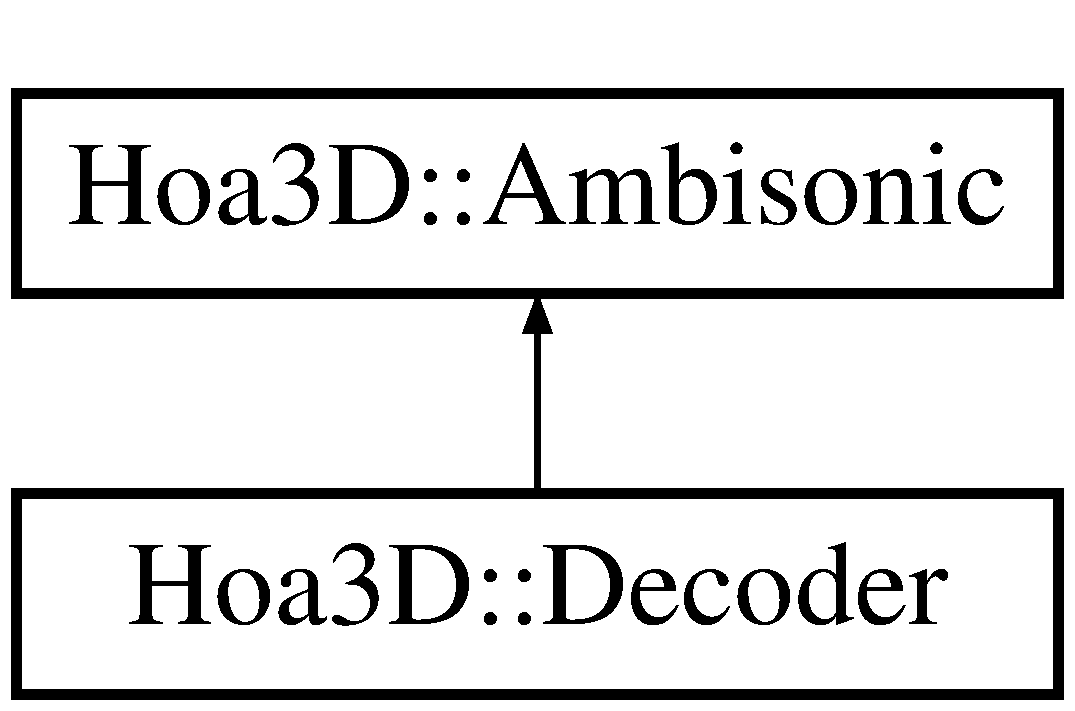
\includegraphics[height=2.000000cm]{class_hoa3_d_1_1_decoder}
\end{center}
\end{figure}
\subsection*{Public Member Functions}
\begin{DoxyCompactItemize}
\item 
\hyperlink{class_hoa3_d_1_1_decoder_aefb3c6a2fd27592480d8198c06ea0968}{Decoder} (unsigned int order, unsigned int number\-Of\-Loudspeakers)
\item 
\hyperlink{class_hoa3_d_1_1_decoder_acc197bebb310a82756ee2061fe371e2d}{$\sim$\-Decoder} ()
\item 
unsigned int \hyperlink{class_hoa3_d_1_1_decoder_a4b14ee0651b397724490de7199d428a7}{get\-Number\-Of\-Loudspeakers} () const 
\begin{DoxyCompactList}\small\item\em This method retrieve the number of loudspeakers. \end{DoxyCompactList}\item 
void \hyperlink{class_hoa3_d_1_1_decoder_ade9c4f54765c1de0f27fadf0b25e88f9}{set\-Loudspeaker\-Position} (unsigned int index, double azimuth, double elevation)
\item 
double \hyperlink{class_hoa3_d_1_1_decoder_a23df7388f6d6b2915566f5aa6d294056}{get\-Loudspeaker\-Azimuth} (unsigned int index) const 
\item 
double \hyperlink{class_hoa3_d_1_1_decoder_aa5102482919297cee85af49991c5984f}{get\-Loudspeaker\-Elevation} (unsigned int index) const 
\item 
void \hyperlink{class_hoa3_d_1_1_decoder_a146f985ebda8e825db2a2ed2cafd5ba6}{process} (const float $\ast$input, float $\ast$output)
\item 
void \hyperlink{class_hoa3_d_1_1_decoder_a2a1931b2fe5c5def0baa9c4d637379a9}{process} (const double $\ast$input, double $\ast$output)
\end{DoxyCompactItemize}


\subsection{Detailed Description}
The ambisonic decoder. 

The decoder should be used to decode a signal encoded in the spherical harmonics domain depending on a decomposition order and a number of loudspeakers. 

Definition at line 18 of file Decoder.\-h.



\subsection{Constructor \& Destructor Documentation}
\hypertarget{class_hoa3_d_1_1_decoder_aefb3c6a2fd27592480d8198c06ea0968}{\index{Hoa3\-D\-::\-Decoder@{Hoa3\-D\-::\-Decoder}!Decoder@{Decoder}}
\index{Decoder@{Decoder}!Hoa3D::Decoder@{Hoa3\-D\-::\-Decoder}}
\subsubsection[{Decoder}]{\setlength{\rightskip}{0pt plus 5cm}Hoa3\-D\-::\-Decoder\-::\-Decoder (
\begin{DoxyParamCaption}
\item[{unsigned int}]{order, }
\item[{unsigned int}]{number\-Of\-Loudspeakers}
\end{DoxyParamCaption}
)}}\label{class_hoa3_d_1_1_decoder_aefb3c6a2fd27592480d8198c06ea0968}
\begin{DoxyVerb}The decoder constructor.
\end{DoxyVerb}
 
\begin{DoxyParams}{Parameters}
{\em order} & The order, must be at least 1. \\
\hline
{\em number\-Of\-Loudspeakers} & The number of loudspeakers, must be at least (order + 1)$^\wedge$2. \\
\hline
{\em shape} & Is a sphere or a half sphere. \\
\hline
\end{DoxyParams}


Definition at line 11 of file Decoder.\-cpp.

\hypertarget{class_hoa3_d_1_1_decoder_acc197bebb310a82756ee2061fe371e2d}{\index{Hoa3\-D\-::\-Decoder@{Hoa3\-D\-::\-Decoder}!$\sim$\-Decoder@{$\sim$\-Decoder}}
\index{$\sim$\-Decoder@{$\sim$\-Decoder}!Hoa3D::Decoder@{Hoa3\-D\-::\-Decoder}}
\subsubsection[{$\sim$\-Decoder}]{\setlength{\rightskip}{0pt plus 5cm}Hoa3\-D\-::\-Decoder\-::$\sim$\-Decoder (
\begin{DoxyParamCaption}
{}
\end{DoxyParamCaption}
)}}\label{class_hoa3_d_1_1_decoder_acc197bebb310a82756ee2061fe371e2d}
The decoder destructor. 

Definition at line 60 of file Decoder.\-cpp.



\subsection{Member Function Documentation}
\hypertarget{class_hoa3_d_1_1_decoder_a23df7388f6d6b2915566f5aa6d294056}{\index{Hoa3\-D\-::\-Decoder@{Hoa3\-D\-::\-Decoder}!get\-Loudspeaker\-Azimuth@{get\-Loudspeaker\-Azimuth}}
\index{get\-Loudspeaker\-Azimuth@{get\-Loudspeaker\-Azimuth}!Hoa3D::Decoder@{Hoa3\-D\-::\-Decoder}}
\subsubsection[{get\-Loudspeaker\-Azimuth}]{\setlength{\rightskip}{0pt plus 5cm}double Hoa3\-D\-::\-Decoder\-::get\-Loudspeaker\-Azimuth (
\begin{DoxyParamCaption}
\item[{unsigned int}]{index}
\end{DoxyParamCaption}
) const}}\label{class_hoa3_d_1_1_decoder_a23df7388f6d6b2915566f5aa6d294056}
\begin{DoxyVerb}Get loudspeaker azimuth value.
\end{DoxyVerb}
 
\begin{DoxyParams}{Parameters}
{\em index} & The index of the loudspeaker. \\
\hline
\end{DoxyParams}
\begin{DoxyReturn}{Returns}
the azimuth value in radians. 
\end{DoxyReturn}
\begin{DoxySeeAlso}{See Also}
\hyperlink{class_hoa3_d_1_1_decoder_aa5102482919297cee85af49991c5984f}{get\-Loudspeaker\-Elevation} 
\end{DoxySeeAlso}


Definition at line 38 of file Decoder.\-cpp.

\hypertarget{class_hoa3_d_1_1_decoder_aa5102482919297cee85af49991c5984f}{\index{Hoa3\-D\-::\-Decoder@{Hoa3\-D\-::\-Decoder}!get\-Loudspeaker\-Elevation@{get\-Loudspeaker\-Elevation}}
\index{get\-Loudspeaker\-Elevation@{get\-Loudspeaker\-Elevation}!Hoa3D::Decoder@{Hoa3\-D\-::\-Decoder}}
\subsubsection[{get\-Loudspeaker\-Elevation}]{\setlength{\rightskip}{0pt plus 5cm}double Hoa3\-D\-::\-Decoder\-::get\-Loudspeaker\-Elevation (
\begin{DoxyParamCaption}
\item[{unsigned int}]{index}
\end{DoxyParamCaption}
) const}}\label{class_hoa3_d_1_1_decoder_aa5102482919297cee85af49991c5984f}
\begin{DoxyVerb}Get loudspeakers elevation value.
\end{DoxyVerb}
 
\begin{DoxyParams}{Parameters}
{\em index} & The index of the loudspeaker. \\
\hline
\end{DoxyParams}
\begin{DoxyReturn}{Returns}
the elevation value in radians. 
\end{DoxyReturn}
\begin{DoxySeeAlso}{See Also}
\hyperlink{class_hoa3_d_1_1_decoder_a23df7388f6d6b2915566f5aa6d294056}{get\-Loudspeaker\-Azimuth} 
\end{DoxySeeAlso}


Definition at line 44 of file Decoder.\-cpp.

\hypertarget{class_hoa3_d_1_1_decoder_a4b14ee0651b397724490de7199d428a7}{\index{Hoa3\-D\-::\-Decoder@{Hoa3\-D\-::\-Decoder}!get\-Number\-Of\-Loudspeakers@{get\-Number\-Of\-Loudspeakers}}
\index{get\-Number\-Of\-Loudspeakers@{get\-Number\-Of\-Loudspeakers}!Hoa3D::Decoder@{Hoa3\-D\-::\-Decoder}}
\subsubsection[{get\-Number\-Of\-Loudspeakers}]{\setlength{\rightskip}{0pt plus 5cm}unsigned int Hoa3\-D\-::\-Decoder\-::get\-Number\-Of\-Loudspeakers (
\begin{DoxyParamCaption}
{}
\end{DoxyParamCaption}
) const\hspace{0.3cm}{\ttfamily [inline]}}}\label{class_hoa3_d_1_1_decoder_a4b14ee0651b397724490de7199d428a7}


This method retrieve the number of loudspeakers. 

Retrieve the number of loudspeakers.

\begin{DoxyReturn}{Returns}
The number of loudspeakers. 
\end{DoxyReturn}


Definition at line 48 of file Decoder.\-h.

\hypertarget{class_hoa3_d_1_1_decoder_a146f985ebda8e825db2a2ed2cafd5ba6}{\index{Hoa3\-D\-::\-Decoder@{Hoa3\-D\-::\-Decoder}!process@{process}}
\index{process@{process}!Hoa3D::Decoder@{Hoa3\-D\-::\-Decoder}}
\subsubsection[{process}]{\setlength{\rightskip}{0pt plus 5cm}void Hoa3\-D\-::\-Decoder\-::process (
\begin{DoxyParamCaption}
\item[{const float $\ast$}]{input, }
\item[{float $\ast$}]{output}
\end{DoxyParamCaption}
)}}\label{class_hoa3_d_1_1_decoder_a146f985ebda8e825db2a2ed2cafd5ba6}
\begin{DoxyVerb}This method performs the decoding with single precision.
\end{DoxyVerb}
 
\begin{DoxyParams}{Parameters}
{\em input} & The inputs array. \\
\hline
{\em outputs} & The output array that contains samples destinated to loudspeakers. \\
\hline
\end{DoxyParams}


Definition at line 50 of file Decoder.\-cpp.

\hypertarget{class_hoa3_d_1_1_decoder_a2a1931b2fe5c5def0baa9c4d637379a9}{\index{Hoa3\-D\-::\-Decoder@{Hoa3\-D\-::\-Decoder}!process@{process}}
\index{process@{process}!Hoa3D::Decoder@{Hoa3\-D\-::\-Decoder}}
\subsubsection[{process}]{\setlength{\rightskip}{0pt plus 5cm}void Hoa3\-D\-::\-Decoder\-::process (
\begin{DoxyParamCaption}
\item[{const double $\ast$}]{input, }
\item[{double $\ast$}]{output}
\end{DoxyParamCaption}
)}}\label{class_hoa3_d_1_1_decoder_a2a1931b2fe5c5def0baa9c4d637379a9}
\begin{DoxyVerb}This method performs the decoding with double precision.
\end{DoxyVerb}
 
\begin{DoxyParams}{Parameters}
{\em input} & The inputs array. \\
\hline
{\em outputs} & The output array that contains samples destinated to loudspeakers. \\
\hline
\end{DoxyParams}


Definition at line 55 of file Decoder.\-cpp.

\hypertarget{class_hoa3_d_1_1_decoder_ade9c4f54765c1de0f27fadf0b25e88f9}{\index{Hoa3\-D\-::\-Decoder@{Hoa3\-D\-::\-Decoder}!set\-Loudspeaker\-Position@{set\-Loudspeaker\-Position}}
\index{set\-Loudspeaker\-Position@{set\-Loudspeaker\-Position}!Hoa3D::Decoder@{Hoa3\-D\-::\-Decoder}}
\subsubsection[{set\-Loudspeaker\-Position}]{\setlength{\rightskip}{0pt plus 5cm}void Hoa3\-D\-::\-Decoder\-::set\-Loudspeaker\-Position (
\begin{DoxyParamCaption}
\item[{unsigned int}]{index, }
\item[{double}]{azimuth, }
\item[{double}]{elevation}
\end{DoxyParamCaption}
)}}\label{class_hoa3_d_1_1_decoder_ade9c4f54765c1de0f27fadf0b25e88f9}
\begin{DoxyVerb}Set loudspeaker position.
\end{DoxyVerb}
 
\begin{DoxyParams}{Parameters}
{\em index} & The index of the loudspeaker. \\
\hline
{\em azimuth} & An azimuth value. In radian, between 0 and 2π. \\
\hline
{\em elevation} & An azimuth value. In radian, between 0 and 2π. \\
\hline
\end{DoxyParams}


Definition at line 22 of file Decoder.\-cpp.



The documentation for this class was generated from the following files\-:\begin{DoxyCompactItemize}
\item 
/\-Users/elioton/\-Documents/programmation/\-C\-I\-C\-M/source\-Tree/\-Hoa\-Library/\-Sources/\-Hoa3\-D/Decoder.\-h\item 
/\-Users/elioton/\-Documents/programmation/\-C\-I\-C\-M/source\-Tree/\-Hoa\-Library/\-Sources/\-Hoa3\-D/Decoder.\-cpp\end{DoxyCompactItemize}

\hypertarget{class_hoa2_d_1_1_decoder}{\section{Hoa2\-D\-:\-:Decoder Class Reference}
\label{class_hoa2_d_1_1_decoder}\index{Hoa2\-D\-::\-Decoder@{Hoa2\-D\-::\-Decoder}}
}
Inheritance diagram for Hoa2\-D\-:\-:Decoder\-:\begin{figure}[H]
\begin{center}
\leavevmode
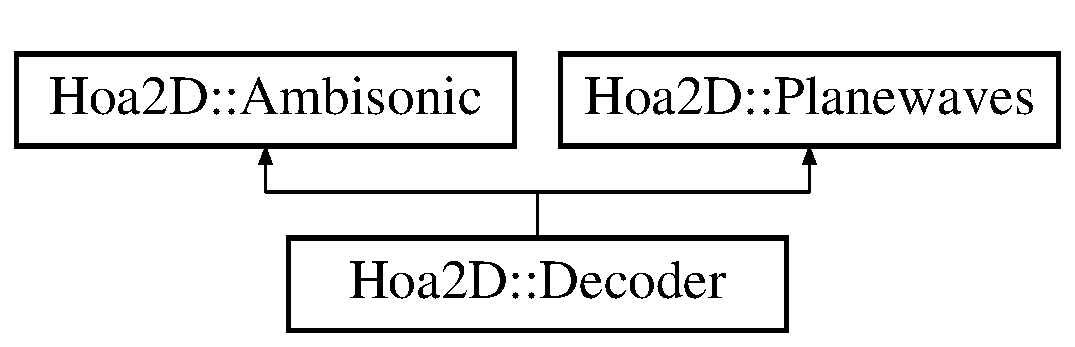
\includegraphics[height=2.000000cm]{class_hoa2_d_1_1_decoder}
\end{center}
\end{figure}
\subsection*{Public Member Functions}
\begin{DoxyCompactItemize}
\item 
\hyperlink{class_hoa2_d_1_1_decoder_a5d7f3ea76e2f50dbfff0e58b48b7cb1b}{Decoder} (unsigned int order, unsigned int number\-Of\-Loudspeakers)
\item 
\hyperlink{class_hoa2_d_1_1_decoder_a2ad3a9bafe6f452bcb378eabd53e0876}{$\sim$\-Decoder} ()
\item 
void \hyperlink{class_hoa2_d_1_1_decoder_a8a4711cff0311450892d268eb60c3a9e}{set\-Loudspeaker\-Position} (unsigned int index, double azimuth)
\item 
double \hyperlink{class_hoa2_d_1_1_decoder_aa07fa3b88a911fb2308fd593397f4bb9}{get\-Loudspeaker\-Azimuth} (unsigned int index) const 
\item 
void \hyperlink{class_hoa2_d_1_1_decoder_a68f00b02c0f8697ecd5364f772bcc9c0}{process} (const float $\ast$input, float $\ast$output)
\item 
void \hyperlink{class_hoa2_d_1_1_decoder_ab3ed928a777ea379b4fa02f65be7e996}{process} (const double $\ast$input, double $\ast$output)
\end{DoxyCompactItemize}


\subsection{Detailed Description}


Definition at line 15 of file Decoder.\-h.



\subsection{Constructor \& Destructor Documentation}
\hypertarget{class_hoa2_d_1_1_decoder_a5d7f3ea76e2f50dbfff0e58b48b7cb1b}{\index{Hoa2\-D\-::\-Decoder@{Hoa2\-D\-::\-Decoder}!Decoder@{Decoder}}
\index{Decoder@{Decoder}!Hoa2D::Decoder@{Hoa2\-D\-::\-Decoder}}
\subsubsection[{Decoder}]{\setlength{\rightskip}{0pt plus 5cm}Hoa2\-D\-::\-Decoder\-::\-Decoder (
\begin{DoxyParamCaption}
\item[{unsigned int}]{order, }
\item[{unsigned int}]{number\-Of\-Loudspeakers}
\end{DoxyParamCaption}
)}}\label{class_hoa2_d_1_1_decoder_a5d7f3ea76e2f50dbfff0e58b48b7cb1b}
\begin{DoxyVerb}The decoder constructor.
\end{DoxyVerb}
 
\begin{DoxyParams}{Parameters}
{\em order} & The order, must be at least 1. \\
\hline
{\em number\-Of\-Loudspeakers} & The number of loudspeakers, must be at least (order + 1)$^\wedge$2. \\
\hline
\end{DoxyParams}


Definition at line 11 of file Decoder.\-cpp.

\hypertarget{class_hoa2_d_1_1_decoder_a2ad3a9bafe6f452bcb378eabd53e0876}{\index{Hoa2\-D\-::\-Decoder@{Hoa2\-D\-::\-Decoder}!$\sim$\-Decoder@{$\sim$\-Decoder}}
\index{$\sim$\-Decoder@{$\sim$\-Decoder}!Hoa2D::Decoder@{Hoa2\-D\-::\-Decoder}}
\subsubsection[{$\sim$\-Decoder}]{\setlength{\rightskip}{0pt plus 5cm}Hoa2\-D\-::\-Decoder\-::$\sim$\-Decoder (
\begin{DoxyParamCaption}
{}
\end{DoxyParamCaption}
)}}\label{class_hoa2_d_1_1_decoder_a2ad3a9bafe6f452bcb378eabd53e0876}
The decoder destructor. 

Definition at line 58 of file Decoder.\-cpp.



\subsection{Member Function Documentation}
\hypertarget{class_hoa2_d_1_1_decoder_aa07fa3b88a911fb2308fd593397f4bb9}{\index{Hoa2\-D\-::\-Decoder@{Hoa2\-D\-::\-Decoder}!get\-Loudspeaker\-Azimuth@{get\-Loudspeaker\-Azimuth}}
\index{get\-Loudspeaker\-Azimuth@{get\-Loudspeaker\-Azimuth}!Hoa2D::Decoder@{Hoa2\-D\-::\-Decoder}}
\subsubsection[{get\-Loudspeaker\-Azimuth}]{\setlength{\rightskip}{0pt plus 5cm}double Hoa2\-D\-::\-Decoder\-::get\-Loudspeaker\-Azimuth (
\begin{DoxyParamCaption}
\item[{unsigned int}]{index}
\end{DoxyParamCaption}
) const}}\label{class_hoa2_d_1_1_decoder_aa07fa3b88a911fb2308fd593397f4bb9}
\begin{DoxyVerb}Get loudspeaker azimuth value.
\end{DoxyVerb}
 
\begin{DoxyParams}{Parameters}
{\em index} & The index of the loudspeaker. \\
\hline
\end{DoxyParams}
\begin{DoxyReturn}{Returns}
the azimuth value in radians. 
\end{DoxyReturn}


Definition at line 42 of file Decoder.\-cpp.

\hypertarget{class_hoa2_d_1_1_decoder_a68f00b02c0f8697ecd5364f772bcc9c0}{\index{Hoa2\-D\-::\-Decoder@{Hoa2\-D\-::\-Decoder}!process@{process}}
\index{process@{process}!Hoa2D::Decoder@{Hoa2\-D\-::\-Decoder}}
\subsubsection[{process}]{\setlength{\rightskip}{0pt plus 5cm}void Hoa2\-D\-::\-Decoder\-::process (
\begin{DoxyParamCaption}
\item[{const float $\ast$}]{input, }
\item[{float $\ast$}]{output}
\end{DoxyParamCaption}
)}}\label{class_hoa2_d_1_1_decoder_a68f00b02c0f8697ecd5364f772bcc9c0}
\begin{DoxyVerb}This method performs the decoding with single precision.
\end{DoxyVerb}
 
\begin{DoxyParams}{Parameters}
{\em input} & The input sample. \\
\hline
{\em outputs} & The output array that contains samples destinated to loudspeakers. \\
\hline
\end{DoxyParams}


Definition at line 48 of file Decoder.\-cpp.

\hypertarget{class_hoa2_d_1_1_decoder_ab3ed928a777ea379b4fa02f65be7e996}{\index{Hoa2\-D\-::\-Decoder@{Hoa2\-D\-::\-Decoder}!process@{process}}
\index{process@{process}!Hoa2D::Decoder@{Hoa2\-D\-::\-Decoder}}
\subsubsection[{process}]{\setlength{\rightskip}{0pt plus 5cm}void Hoa2\-D\-::\-Decoder\-::process (
\begin{DoxyParamCaption}
\item[{const double $\ast$}]{input, }
\item[{double $\ast$}]{output}
\end{DoxyParamCaption}
)}}\label{class_hoa2_d_1_1_decoder_ab3ed928a777ea379b4fa02f65be7e996}
\begin{DoxyVerb}This method performs the decoding with double precision.
\end{DoxyVerb}
 
\begin{DoxyParams}{Parameters}
{\em input} & The input sample. \\
\hline
{\em outputs} & The output array that contains samples destinated to loudspeakers. \\
\hline
\end{DoxyParams}


Definition at line 53 of file Decoder.\-cpp.

\hypertarget{class_hoa2_d_1_1_decoder_a8a4711cff0311450892d268eb60c3a9e}{\index{Hoa2\-D\-::\-Decoder@{Hoa2\-D\-::\-Decoder}!set\-Loudspeaker\-Position@{set\-Loudspeaker\-Position}}
\index{set\-Loudspeaker\-Position@{set\-Loudspeaker\-Position}!Hoa2D::Decoder@{Hoa2\-D\-::\-Decoder}}
\subsubsection[{set\-Loudspeaker\-Position}]{\setlength{\rightskip}{0pt plus 5cm}void Hoa2\-D\-::\-Decoder\-::set\-Loudspeaker\-Position (
\begin{DoxyParamCaption}
\item[{unsigned int}]{index, }
\item[{double}]{azimuth}
\end{DoxyParamCaption}
)}}\label{class_hoa2_d_1_1_decoder_a8a4711cff0311450892d268eb60c3a9e}
\begin{DoxyVerb}Set loudspeaker position.
\end{DoxyVerb}
 
\begin{DoxyParams}{Parameters}
{\em index} & The index of the loudspeaker. \\
\hline
{\em azimuth} & An azimuth value. In radian, between 0 and 2π. \\
\hline
\end{DoxyParams}


Definition at line 27 of file Decoder.\-cpp.



The documentation for this class was generated from the following files\-:\begin{DoxyCompactItemize}
\item 
/\-Users/elioton/\-Documents/programmation/\-C\-I\-C\-M/source\-Tree/\-Hoa\-Library/\-Sources/\-Hoa2\-D/Decoder.\-h\item 
/\-Users/elioton/\-Documents/programmation/\-C\-I\-C\-M/source\-Tree/\-Hoa\-Library/\-Sources/\-Hoa2\-D/Decoder.\-cpp\end{DoxyCompactItemize}

\hypertarget{class_hoa2_d_1_1_encoder}{\section{Hoa2\-D\-:\-:Encoder Class Reference}
\label{class_hoa2_d_1_1_encoder}\index{Hoa2\-D\-::\-Encoder@{Hoa2\-D\-::\-Encoder}}
}


The ambisonic encoder.  




{\ttfamily \#include $<$Encoder.\-h$>$}

Inheritance diagram for Hoa2\-D\-:\-:Encoder\-:\begin{figure}[H]
\begin{center}
\leavevmode
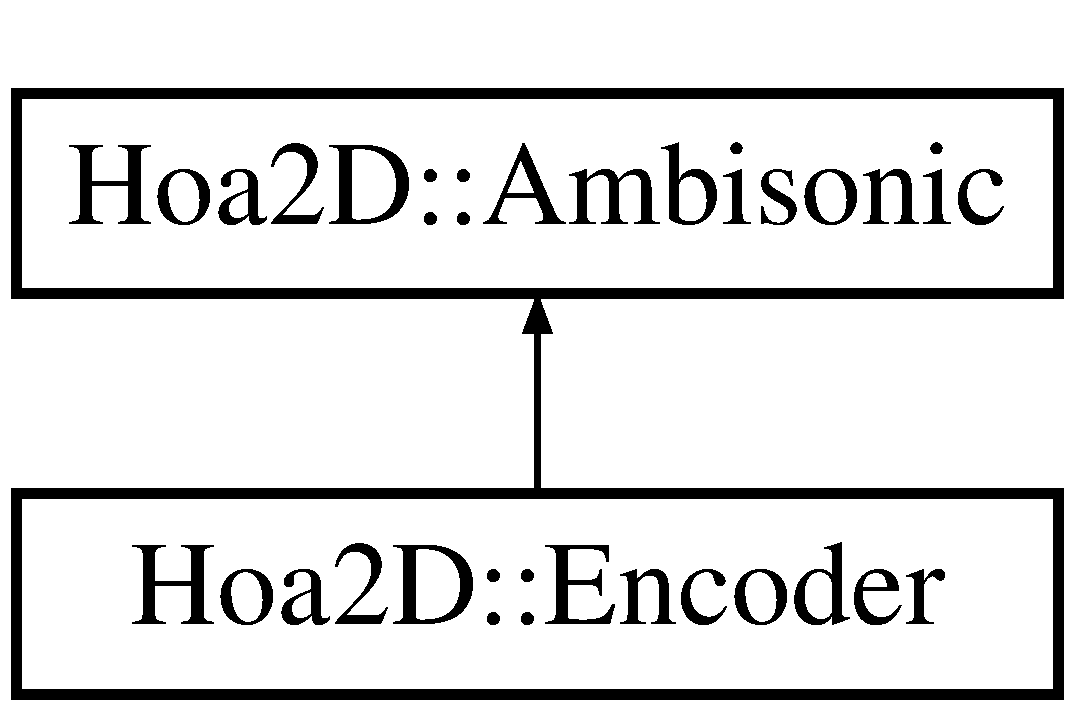
\includegraphics[height=2.000000cm]{class_hoa2_d_1_1_encoder}
\end{center}
\end{figure}
\subsection*{Public Member Functions}
\begin{DoxyCompactItemize}
\item 
\hyperlink{class_hoa2_d_1_1_encoder_a3387c0cd62d3af13ef851d5372c55a6f}{Encoder} (unsigned int order)
\begin{DoxyCompactList}\small\item\em The encoder constructor. \end{DoxyCompactList}\item 
\hyperlink{class_hoa2_d_1_1_encoder_a1faf86f0a74e68d91cd92608b5fd37c8}{$\sim$\-Encoder} ()
\begin{DoxyCompactList}\small\item\em The encoder destructor. \end{DoxyCompactList}\item 
void \hyperlink{class_hoa2_d_1_1_encoder_acc60cfd737fe1f0866e7d464ef1ec1f8}{set\-Azimuth} (const double azimuth)
\begin{DoxyCompactList}\small\item\em This method set the angle of azimuth. \end{DoxyCompactList}\item 
double \hyperlink{class_hoa2_d_1_1_encoder_a2ed07d913b444c58b3b1cf75dd1df117}{get\-Azimuth} () const 
\begin{DoxyCompactList}\small\item\em This method performs the encoding with single precision. \end{DoxyCompactList}\item 
void \hyperlink{class_hoa2_d_1_1_encoder_a2d12e80e9a7a59970972dca6b444b6bc}{process} (const float input, float $\ast$outputs)
\begin{DoxyCompactList}\small\item\em This method performs the encoding with single precision. \end{DoxyCompactList}\item 
void \hyperlink{class_hoa2_d_1_1_encoder_a235cc53dbf4fcbe71b3ea72a721eea81}{process} (const double input, double $\ast$outputs)
\begin{DoxyCompactList}\small\item\em This method performs the encoding with double precision. \end{DoxyCompactList}\end{DoxyCompactItemize}


\subsection{Detailed Description}
The ambisonic encoder. 

The encoder should be used to encode a signal in the spherical harmonics domain depending of an order of decomposition. It allows to control the azimuth of the encoding. 

Definition at line 17 of file Encoder.\-h.



\subsection{Constructor \& Destructor Documentation}
\hypertarget{class_hoa2_d_1_1_encoder_a3387c0cd62d3af13ef851d5372c55a6f}{\index{Hoa2\-D\-::\-Encoder@{Hoa2\-D\-::\-Encoder}!Encoder@{Encoder}}
\index{Encoder@{Encoder}!Hoa2D::Encoder@{Hoa2\-D\-::\-Encoder}}
\subsubsection[{Encoder}]{\setlength{\rightskip}{0pt plus 5cm}Hoa2\-D\-::\-Encoder\-::\-Encoder (
\begin{DoxyParamCaption}
\item[{unsigned int}]{order}
\end{DoxyParamCaption}
)}}\label{class_hoa2_d_1_1_encoder_a3387c0cd62d3af13ef851d5372c55a6f}


The encoder constructor. 

The encoder constructor allocates and initialize the member values to computes spherical harmonics coefficients depending of a decomposition order. The order must be at least 1.


\begin{DoxyParams}{Parameters}
{\em order} & The order. \\
\hline
\end{DoxyParams}


Definition at line 11 of file Encoder.\-cpp.

\hypertarget{class_hoa2_d_1_1_encoder_a1faf86f0a74e68d91cd92608b5fd37c8}{\index{Hoa2\-D\-::\-Encoder@{Hoa2\-D\-::\-Encoder}!$\sim$\-Encoder@{$\sim$\-Encoder}}
\index{$\sim$\-Encoder@{$\sim$\-Encoder}!Hoa2D::Encoder@{Hoa2\-D\-::\-Encoder}}
\subsubsection[{$\sim$\-Encoder}]{\setlength{\rightskip}{0pt plus 5cm}Hoa2\-D\-::\-Encoder\-::$\sim$\-Encoder (
\begin{DoxyParamCaption}
{}
\end{DoxyParamCaption}
)}}\label{class_hoa2_d_1_1_encoder_a1faf86f0a74e68d91cd92608b5fd37c8}


The encoder destructor. 

The encoder destructor free the memory. 

Definition at line 56 of file Encoder.\-cpp.



\subsection{Member Function Documentation}
\hypertarget{class_hoa2_d_1_1_encoder_a2ed07d913b444c58b3b1cf75dd1df117}{\index{Hoa2\-D\-::\-Encoder@{Hoa2\-D\-::\-Encoder}!get\-Azimuth@{get\-Azimuth}}
\index{get\-Azimuth@{get\-Azimuth}!Hoa2D::Encoder@{Hoa2\-D\-::\-Encoder}}
\subsubsection[{get\-Azimuth}]{\setlength{\rightskip}{0pt plus 5cm}double Hoa2\-D\-::\-Encoder\-::get\-Azimuth (
\begin{DoxyParamCaption}
{}
\end{DoxyParamCaption}
) const\hspace{0.3cm}{\ttfamily [inline]}}}\label{class_hoa2_d_1_1_encoder_a2ed07d913b444c58b3b1cf75dd1df117}


This method performs the encoding with single precision. 

You should use this method for in-\/place or not-\/in-\/place processing and performs the encoding sample by sample. The outputs array contains the spherical harmonics samples and the minimum size must be the number of harmonics.


\begin{DoxyParams}{Parameters}
{\em input} & The input sample. \\
\hline
{\em outputs} & The output array.\-Get the yaw value (rotation on the z-\/axis). The yaw is equivalent to a rotation on the z-\/axis (also named rotation).\\
\hline
\end{DoxyParams}
\begin{DoxyReturn}{Returns}
value The yaw value between 0 and 2π. 
\end{DoxyReturn}


Definition at line 59 of file Encoder.\-h.

\hypertarget{class_hoa2_d_1_1_encoder_a2d12e80e9a7a59970972dca6b444b6bc}{\index{Hoa2\-D\-::\-Encoder@{Hoa2\-D\-::\-Encoder}!process@{process}}
\index{process@{process}!Hoa2D::Encoder@{Hoa2\-D\-::\-Encoder}}
\subsubsection[{process}]{\setlength{\rightskip}{0pt plus 5cm}void Hoa2\-D\-::\-Encoder\-::process (
\begin{DoxyParamCaption}
\item[{const float}]{input, }
\item[{float $\ast$}]{outputs}
\end{DoxyParamCaption}
)}}\label{class_hoa2_d_1_1_encoder_a2d12e80e9a7a59970972dca6b444b6bc}


This method performs the encoding with single precision. 

\begin{DoxyVerb}You should use this method for in-place or not-in-place processing and performs the encoding sample by sample. The outputs array contains the spherical harmonics samples and the minimum size must be the number of harmonics.
\end{DoxyVerb}



\begin{DoxyParams}{Parameters}
{\em input} & The input sample. \\
\hline
{\em outputs} & The output array. \\
\hline
\end{DoxyParams}


Definition at line 24 of file Encoder.\-cpp.

\hypertarget{class_hoa2_d_1_1_encoder_a235cc53dbf4fcbe71b3ea72a721eea81}{\index{Hoa2\-D\-::\-Encoder@{Hoa2\-D\-::\-Encoder}!process@{process}}
\index{process@{process}!Hoa2D::Encoder@{Hoa2\-D\-::\-Encoder}}
\subsubsection[{process}]{\setlength{\rightskip}{0pt plus 5cm}void Hoa2\-D\-::\-Encoder\-::process (
\begin{DoxyParamCaption}
\item[{const double}]{input, }
\item[{double $\ast$}]{outputs}
\end{DoxyParamCaption}
)}}\label{class_hoa2_d_1_1_encoder_a235cc53dbf4fcbe71b3ea72a721eea81}


This method performs the encoding with double precision. 

You should use this method for in-\/place or not-\/in-\/place processing and performs the encoding sample by sample. The outputs array contains the spherical harmonics samples and the minimum size must be the number of harmonics.


\begin{DoxyParams}{Parameters}
{\em input} & The input sample. \\
\hline
{\em outputs} & The output array. \\
\hline
\end{DoxyParams}


Definition at line 40 of file Encoder.\-cpp.

\hypertarget{class_hoa2_d_1_1_encoder_acc60cfd737fe1f0866e7d464ef1ec1f8}{\index{Hoa2\-D\-::\-Encoder@{Hoa2\-D\-::\-Encoder}!set\-Azimuth@{set\-Azimuth}}
\index{set\-Azimuth@{set\-Azimuth}!Hoa2D::Encoder@{Hoa2\-D\-::\-Encoder}}
\subsubsection[{set\-Azimuth}]{\setlength{\rightskip}{0pt plus 5cm}void Hoa2\-D\-::\-Encoder\-::set\-Azimuth (
\begin{DoxyParamCaption}
\item[{const double}]{azimuth}
\end{DoxyParamCaption}
)}}\label{class_hoa2_d_1_1_encoder_acc60cfd737fe1f0866e7d464ef1ec1f8}


This method set the angle of azimuth. 

The angle of azimuth in radian and you should prefer to use it between 0 and 2 Pi to avoid recursive wrapping of the value. The direction of rotation is counterclockwise. The 0 radian is Pi/2 phase shifted relative to a mathematical representation of a circle, then the 0 radian is at the \char`\"{}front\char`\"{} of the soundfield.


\begin{DoxyParams}{Parameters}
{\em azimuth} & The azimuth. \\
\hline
\end{DoxyParams}


Definition at line 17 of file Encoder.\-cpp.



The documentation for this class was generated from the following files\-:\begin{DoxyCompactItemize}
\item 
/\-Users/\-Pierre/\-Source\-Tree/\-Hoa\-Library/\-Sources/\-Hoa2\-D/Encoder.\-h\item 
/\-Users/\-Pierre/\-Source\-Tree/\-Hoa\-Library/\-Sources/\-Hoa2\-D/Encoder.\-cpp\end{DoxyCompactItemize}

\hypertarget{class_hoa3_d_1_1_encoder}{\section{Hoa3\-D\-:\-:Encoder Class Reference}
\label{class_hoa3_d_1_1_encoder}\index{Hoa3\-D\-::\-Encoder@{Hoa3\-D\-::\-Encoder}}
}


The ambisonic encoder.  




{\ttfamily \#include $<$Encoder.\-h$>$}

Inheritance diagram for Hoa3\-D\-:\-:Encoder\-:\begin{figure}[H]
\begin{center}
\leavevmode
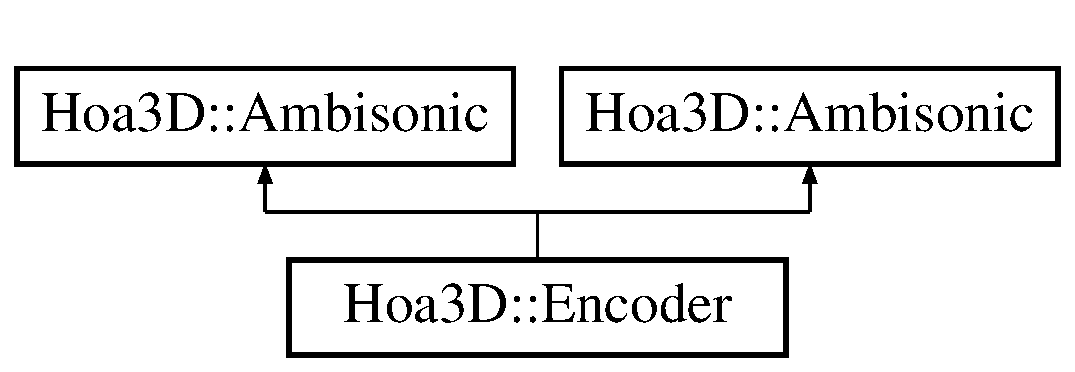
\includegraphics[height=2.000000cm]{class_hoa3_d_1_1_encoder}
\end{center}
\end{figure}
\subsection*{Public Member Functions}
\begin{DoxyCompactItemize}
\item 
\hyperlink{class_hoa3_d_1_1_encoder_a71052bcb0cbcf600852423c8cbbf29ce}{Encoder} (unsigned int order)
\begin{DoxyCompactList}\small\item\em The encoder constructor. \end{DoxyCompactList}\item 
\hyperlink{class_hoa3_d_1_1_encoder_a9842ee9f5abcba58a05a98dbfdff1b15}{$\sim$\-Encoder} ()
\begin{DoxyCompactList}\small\item\em The encoder destructor. \end{DoxyCompactList}\item 
void \hyperlink{class_hoa3_d_1_1_encoder_a7dbf4d5791003ed486fc0b5462409e0a}{set\-Azimuth} (const double azimuth)
\begin{DoxyCompactList}\small\item\em This method set the angle of azimuth. \end{DoxyCompactList}\item 
void \hyperlink{class_hoa3_d_1_1_encoder_a3bf01c6ecd90108c66c19ce7e5bde97d}{set\-Elevation} (const double elevation)
\begin{DoxyCompactList}\small\item\em This method set the angle of elevation. \end{DoxyCompactList}\item 
double \hyperlink{class_hoa3_d_1_1_encoder_a9887680a1cd725b96db8d83297922ae2}{get\-Normalization} (const unsigned int index) const 
\item 
void \hyperlink{class_hoa3_d_1_1_encoder_aedcd6cc5a50c85f373c61137e452a9b4}{process} (const float input, float $\ast$outputs)
\begin{DoxyCompactList}\small\item\em This method performs the encoding with single precision. \end{DoxyCompactList}\item 
void \hyperlink{class_hoa3_d_1_1_encoder_a6a8a7c7219424dd74bb5180a5b2c25e3}{process} (const double input, double $\ast$outputs)
\begin{DoxyCompactList}\small\item\em This method performs the encoding with double precision. \end{DoxyCompactList}\end{DoxyCompactItemize}


\subsection{Detailed Description}
The ambisonic encoder. 

The encoder should be used to encode a signal in the spherical harmonics domain depending of an order of decomposition. It allows to control the azimuth and the elevation of the encoding. If you want to spatialize with distance compensation, you should use the \hyperlink{class_hoa3_d_1_1_map}{Map} class.

\begin{DoxySeeAlso}{See Also}
\hyperlink{class_hoa3_d_1_1_map}{Map} 
\end{DoxySeeAlso}


Definition at line 19 of file Encoder.\-h.



\subsection{Constructor \& Destructor Documentation}
\hypertarget{class_hoa3_d_1_1_encoder_a71052bcb0cbcf600852423c8cbbf29ce}{\index{Hoa3\-D\-::\-Encoder@{Hoa3\-D\-::\-Encoder}!Encoder@{Encoder}}
\index{Encoder@{Encoder}!Hoa3D::Encoder@{Hoa3\-D\-::\-Encoder}}
\subsubsection[{Encoder}]{\setlength{\rightskip}{0pt plus 5cm}Hoa3\-D\-::\-Encoder\-::\-Encoder (
\begin{DoxyParamCaption}
\item[{unsigned int}]{order}
\end{DoxyParamCaption}
)}}\label{class_hoa3_d_1_1_encoder_a71052bcb0cbcf600852423c8cbbf29ce}


The encoder constructor. 

The encoder constructor allocates and initialize the member values to computes spherical harmonics coefficients depending of a decomposition order. The order must be at least 1.


\begin{DoxyParams}{Parameters}
{\em order} & The order. \\
\hline
\end{DoxyParams}


Definition at line 11 of file Encoder.\-cpp.

\hypertarget{class_hoa3_d_1_1_encoder_a9842ee9f5abcba58a05a98dbfdff1b15}{\index{Hoa3\-D\-::\-Encoder@{Hoa3\-D\-::\-Encoder}!$\sim$\-Encoder@{$\sim$\-Encoder}}
\index{$\sim$\-Encoder@{$\sim$\-Encoder}!Hoa3D::Encoder@{Hoa3\-D\-::\-Encoder}}
\subsubsection[{$\sim$\-Encoder}]{\setlength{\rightskip}{0pt plus 5cm}Hoa3\-D\-::\-Encoder\-::$\sim$\-Encoder (
\begin{DoxyParamCaption}
{}
\end{DoxyParamCaption}
)}}\label{class_hoa3_d_1_1_encoder_a9842ee9f5abcba58a05a98dbfdff1b15}


The encoder destructor. 

The encoder destructor free the memory. 

Definition at line 116 of file Encoder.\-cpp.



\subsection{Member Function Documentation}
\hypertarget{class_hoa3_d_1_1_encoder_a9887680a1cd725b96db8d83297922ae2}{\index{Hoa3\-D\-::\-Encoder@{Hoa3\-D\-::\-Encoder}!get\-Normalization@{get\-Normalization}}
\index{get\-Normalization@{get\-Normalization}!Hoa3D::Encoder@{Hoa3\-D\-::\-Encoder}}
\subsubsection[{get\-Normalization}]{\setlength{\rightskip}{0pt plus 5cm}double Hoa3\-D\-::\-Encoder\-::get\-Normalization (
\begin{DoxyParamCaption}
\item[{const unsigned int}]{index}
\end{DoxyParamCaption}
) const\hspace{0.3cm}{\ttfamily [inline]}}}\label{class_hoa3_d_1_1_encoder_a9887680a1cd725b96db8d83297922ae2}
Retreive the normalization of an harmonics


\begin{DoxyParams}{Parameters}
{\em index} & The index of the harmonics. \\
\hline
\end{DoxyParams}


Definition at line 63 of file Encoder.\-h.

\hypertarget{class_hoa3_d_1_1_encoder_aedcd6cc5a50c85f373c61137e452a9b4}{\index{Hoa3\-D\-::\-Encoder@{Hoa3\-D\-::\-Encoder}!process@{process}}
\index{process@{process}!Hoa3D::Encoder@{Hoa3\-D\-::\-Encoder}}
\subsubsection[{process}]{\setlength{\rightskip}{0pt plus 5cm}void Hoa3\-D\-::\-Encoder\-::process (
\begin{DoxyParamCaption}
\item[{const float}]{input, }
\item[{float $\ast$}]{outputs}
\end{DoxyParamCaption}
)}}\label{class_hoa3_d_1_1_encoder_aedcd6cc5a50c85f373c61137e452a9b4}


This method performs the encoding with single precision. 

You should use this method for in-\/place or not-\/in-\/place processing and performs the encoding sample by sample. The outputs array contains the spherical harmonics samples and the minimum size must be the number of harmonics.


\begin{DoxyParams}{Parameters}
{\em input} & The input sample. \\
\hline
{\em outputs} & The outputs array. \\
\hline
\end{DoxyParams}


Definition at line 70 of file Encoder.\-cpp.

\hypertarget{class_hoa3_d_1_1_encoder_a6a8a7c7219424dd74bb5180a5b2c25e3}{\index{Hoa3\-D\-::\-Encoder@{Hoa3\-D\-::\-Encoder}!process@{process}}
\index{process@{process}!Hoa3D::Encoder@{Hoa3\-D\-::\-Encoder}}
\subsubsection[{process}]{\setlength{\rightskip}{0pt plus 5cm}void Hoa3\-D\-::\-Encoder\-::process (
\begin{DoxyParamCaption}
\item[{const double}]{input, }
\item[{double $\ast$}]{outputs}
\end{DoxyParamCaption}
)}}\label{class_hoa3_d_1_1_encoder_a6a8a7c7219424dd74bb5180a5b2c25e3}


This method performs the encoding with double precision. 

You should use this method for in-\/place or not-\/in-\/place processing and performs the encoding sample by sample. The outputs array contains the spherical harmonics samples and the minimum size must be the number of harmonics.


\begin{DoxyParams}{Parameters}
{\em input} & The input sample. \\
\hline
{\em outputs} & The outputs array. \\
\hline
\end{DoxyParams}


Definition at line 92 of file Encoder.\-cpp.

\hypertarget{class_hoa3_d_1_1_encoder_a7dbf4d5791003ed486fc0b5462409e0a}{\index{Hoa3\-D\-::\-Encoder@{Hoa3\-D\-::\-Encoder}!set\-Azimuth@{set\-Azimuth}}
\index{set\-Azimuth@{set\-Azimuth}!Hoa3D::Encoder@{Hoa3\-D\-::\-Encoder}}
\subsubsection[{set\-Azimuth}]{\setlength{\rightskip}{0pt plus 5cm}void Hoa3\-D\-::\-Encoder\-::set\-Azimuth (
\begin{DoxyParamCaption}
\item[{const double}]{azimuth}
\end{DoxyParamCaption}
)}}\label{class_hoa3_d_1_1_encoder_a7dbf4d5791003ed486fc0b5462409e0a}


This method set the angle of azimuth. 

The angle of azimuth in radian and you should prefer to use it between 0 and 2 Pi to avoid recursive wrapping of the value. The direction of rotation is counterclockwise. The 0 radian is Pi/2 phase shifted relative to a mathematical representation of a circle, then the 0 radian is at the \char`\"{}front\char`\"{} of the soundfield.


\begin{DoxyParams}{Parameters}
{\em azimuth} & The azimuth. \\
\hline
\end{DoxyParams}
\begin{DoxySeeAlso}{See Also}
\hyperlink{class_hoa3_d_1_1_encoder_a3bf01c6ecd90108c66c19ce7e5bde97d}{set\-Elevation()} 
\end{DoxySeeAlso}


Definition at line 60 of file Encoder.\-cpp.

\hypertarget{class_hoa3_d_1_1_encoder_a3bf01c6ecd90108c66c19ce7e5bde97d}{\index{Hoa3\-D\-::\-Encoder@{Hoa3\-D\-::\-Encoder}!set\-Elevation@{set\-Elevation}}
\index{set\-Elevation@{set\-Elevation}!Hoa3D::Encoder@{Hoa3\-D\-::\-Encoder}}
\subsubsection[{set\-Elevation}]{\setlength{\rightskip}{0pt plus 5cm}void Hoa3\-D\-::\-Encoder\-::set\-Elevation (
\begin{DoxyParamCaption}
\item[{const double}]{elevation}
\end{DoxyParamCaption}
)}}\label{class_hoa3_d_1_1_encoder_a3bf01c6ecd90108c66c19ce7e5bde97d}


This method set the angle of elevation. 

The angle of elevation in radian and you should prefer to use it between 0 and 2 Pi to avoid recursive wrapping of the value. The direction of rotation is from bottom to the top. The 0 radian is centered at the \char`\"{}front\char`\"{} of the soundfield, then Pi/2 is at the top, -\/\-Pi/2 is at the bottom and Pi is behind. Note that if the angle of elevation is between Pi/2 and 3$\ast$\-Pi/2, the azimuth is reversed.


\begin{DoxyParams}{Parameters}
{\em elevation} & The elevation. \\
\hline
\end{DoxyParams}
\begin{DoxySeeAlso}{See Also}
\hyperlink{class_hoa3_d_1_1_encoder_a3bf01c6ecd90108c66c19ce7e5bde97d}{set\-Elevation()} 
\end{DoxySeeAlso}


Definition at line 65 of file Encoder.\-cpp.



The documentation for this class was generated from the following files\-:\begin{DoxyCompactItemize}
\item 
/\-Users/\-Pierre/\-Source\-Tree/\-Hoa\-Library/\-Sources/\-Hoa3\-D/Encoder.\-h\item 
/\-Users/\-Pierre/\-Source\-Tree/\-Hoa\-Library/\-Sources/\-Hoa3\-D/Encoder.\-cpp\end{DoxyCompactItemize}

\hypertarget{class_hoa3_d_1_1_map}{\section{Hoa3\-D\-:\-:Map Class Reference}
\label{class_hoa3_d_1_1_map}\index{Hoa3\-D\-::\-Map@{Hoa3\-D\-::\-Map}}
}


The ambisonic multi-\/encoder with distance compensation.  




{\ttfamily \#include $<$Map.\-h$>$}

Inheritance diagram for Hoa3\-D\-:\-:Map\-:\begin{figure}[H]
\begin{center}
\leavevmode
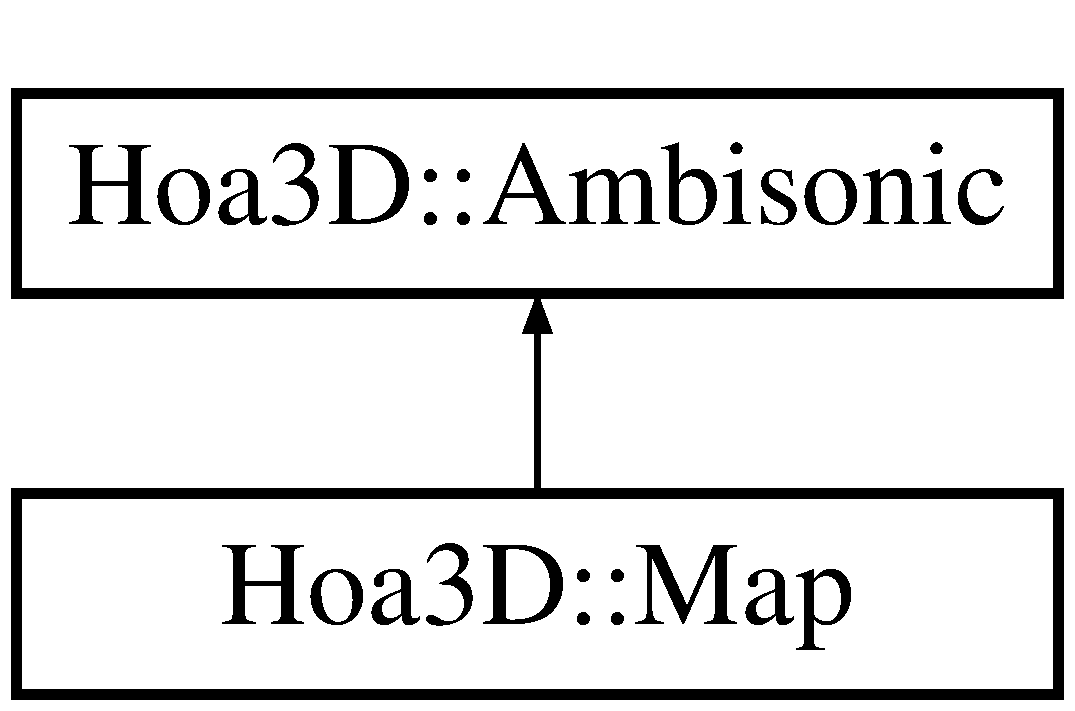
\includegraphics[height=2.000000cm]{class_hoa3_d_1_1_map}
\end{center}
\end{figure}
\subsection*{Public Member Functions}
\begin{DoxyCompactItemize}
\item 
\hyperlink{class_hoa3_d_1_1_map_a442cdcc3ac651b716ae2617fa64c44b4}{Map} (unsigned int order, unsigned int number\-Of\-Sources)
\begin{DoxyCompactList}\small\item\em The map constructor. \end{DoxyCompactList}\item 
\hyperlink{class_hoa3_d_1_1_map_a89f5772a7f26cda206637dd1fca1c16e}{$\sim$\-Map} ()
\begin{DoxyCompactList}\small\item\em The map destructor. \end{DoxyCompactList}\item 
void \hyperlink{class_hoa3_d_1_1_map_a251f215d1e137e652d12fc8e811bd8c8}{set\-Azimuth} (unsigned int index, const double azimuth)
\begin{DoxyCompactList}\small\item\em This method set the angle of azimuth of a source. \end{DoxyCompactList}\item 
void \hyperlink{class_hoa3_d_1_1_map_a03262a011f73ed57ba40bb6fe6d50814}{set\-Elevation} (unsigned int index, const double elevation)
\begin{DoxyCompactList}\small\item\em This method set the angle of elevation of a source. \end{DoxyCompactList}\item 
void \hyperlink{class_hoa3_d_1_1_map_a61b55ea17301701fc02dffca46957330}{set\-Distance} (unsigned int index, const double distance)
\begin{DoxyCompactList}\small\item\em This method set the diatnce of a source. \end{DoxyCompactList}\item 
unsigned int \hyperlink{class_hoa3_d_1_1_map_a49c97eaf507f6ccc9c1e7eb8fbff0ac9}{get\-Number\-Of\-Sources} () const 
\begin{DoxyCompactList}\small\item\em This method retrieve the number of sources. \end{DoxyCompactList}\item 
void \hyperlink{class_hoa3_d_1_1_map_af332c122731c3df55c3dcf56d39c7941}{process} (const float $\ast$inputs, float $\ast$outputs)
\begin{DoxyCompactList}\small\item\em This method performs the encoding with distance compensation with single precision. \end{DoxyCompactList}\item 
void \hyperlink{class_hoa3_d_1_1_map_a53a82b55c1ec5e52c2ab788984c5c2d0}{process} (const double $\ast$inputs, double $\ast$outputs)
\begin{DoxyCompactList}\small\item\em This method performs the encoding with distance compensation with double precision. \end{DoxyCompactList}\end{DoxyCompactItemize}


\subsection{Detailed Description}
The ambisonic multi-\/encoder with distance compensation. 

The map is a multi \hyperlink{class_hoa3_d_1_1_encoder}{Encoder} with distance compensation. It uses intances of the \hyperlink{class_hoa3_d_1_1_wider}{Wider} class to decrease the directionnality of sources by simulating fractionnal orders when the sources are inside the ambisonic sphere and a simple diminution of the gain when the sources get away from the ambisonic sphere.

\begin{DoxySeeAlso}{See Also}
\hyperlink{class_hoa3_d_1_1_encoder}{Encoder} 
\end{DoxySeeAlso}


Definition at line 21 of file Map.\-h.



\subsection{Constructor \& Destructor Documentation}
\hypertarget{class_hoa3_d_1_1_map_a442cdcc3ac651b716ae2617fa64c44b4}{\index{Hoa3\-D\-::\-Map@{Hoa3\-D\-::\-Map}!Map@{Map}}
\index{Map@{Map}!Hoa3D::Map@{Hoa3\-D\-::\-Map}}
\subsubsection[{Map}]{\setlength{\rightskip}{0pt plus 5cm}Hoa3\-D\-::\-Map\-::\-Map (
\begin{DoxyParamCaption}
\item[{unsigned int}]{order, }
\item[{unsigned int}]{number\-Of\-Sources}
\end{DoxyParamCaption}
)}}\label{class_hoa3_d_1_1_map_a442cdcc3ac651b716ae2617fa64c44b4}


The map constructor. 

The map constructor allocates and initialize the member values and classes depending of a decomposition order and the number of sources. The order and the number of sources must be at least 1.


\begin{DoxyParams}{Parameters}
{\em order} & The order. \\
\hline
{\em number\-Of\-Sources} & The number of sources. \\
\hline
\end{DoxyParams}


Definition at line 11 of file Map.\-cpp.

\hypertarget{class_hoa3_d_1_1_map_a89f5772a7f26cda206637dd1fca1c16e}{\index{Hoa3\-D\-::\-Map@{Hoa3\-D\-::\-Map}!$\sim$\-Map@{$\sim$\-Map}}
\index{$\sim$\-Map@{$\sim$\-Map}!Hoa3D::Map@{Hoa3\-D\-::\-Map}}
\subsubsection[{$\sim$\-Map}]{\setlength{\rightskip}{0pt plus 5cm}Hoa3\-D\-::\-Map\-::$\sim$\-Map (
\begin{DoxyParamCaption}
{}
\end{DoxyParamCaption}
)}}\label{class_hoa3_d_1_1_map_a89f5772a7f26cda206637dd1fca1c16e}


The map destructor. 

The map destructor free the memory and deallocate the member classes. 

Definition at line 77 of file Map.\-cpp.



\subsection{Member Function Documentation}
\hypertarget{class_hoa3_d_1_1_map_a49c97eaf507f6ccc9c1e7eb8fbff0ac9}{\index{Hoa3\-D\-::\-Map@{Hoa3\-D\-::\-Map}!get\-Number\-Of\-Sources@{get\-Number\-Of\-Sources}}
\index{get\-Number\-Of\-Sources@{get\-Number\-Of\-Sources}!Hoa3D::Map@{Hoa3\-D\-::\-Map}}
\subsubsection[{get\-Number\-Of\-Sources}]{\setlength{\rightskip}{0pt plus 5cm}unsigned int Hoa3\-D\-::\-Map\-::get\-Number\-Of\-Sources (
\begin{DoxyParamCaption}
{}
\end{DoxyParamCaption}
) const\hspace{0.3cm}{\ttfamily [inline]}}}\label{class_hoa3_d_1_1_map_a49c97eaf507f6ccc9c1e7eb8fbff0ac9}


This method retrieve the number of sources. 

Retrieve the number of sources.

\begin{DoxyReturn}{Returns}
The number of sources. 
\end{DoxyReturn}


Definition at line 83 of file Map.\-h.

\hypertarget{class_hoa3_d_1_1_map_af332c122731c3df55c3dcf56d39c7941}{\index{Hoa3\-D\-::\-Map@{Hoa3\-D\-::\-Map}!process@{process}}
\index{process@{process}!Hoa3D::Map@{Hoa3\-D\-::\-Map}}
\subsubsection[{process}]{\setlength{\rightskip}{0pt plus 5cm}void Hoa3\-D\-::\-Map\-::process (
\begin{DoxyParamCaption}
\item[{const float $\ast$}]{inputs, }
\item[{float $\ast$}]{outputs}
\end{DoxyParamCaption}
)}}\label{class_hoa3_d_1_1_map_af332c122731c3df55c3dcf56d39c7941}


This method performs the encoding with distance compensation with single precision. 

You should use this method for in-\/place or not-\/in-\/place processing and performs the encoding with distance compensation sample by sample. The inputs array contains the samples of the sources and the minimum size sould be the number of sources. The outputs array contains the spherical harmonics samples and the minimum size must be the number of harmonics.


\begin{DoxyParams}{Parameters}
{\em inputs} & The inputs array. \\
\hline
{\em outputs} & The outputs array. \\
\hline
\end{DoxyParams}


Definition at line 53 of file Map.\-cpp.

\hypertarget{class_hoa3_d_1_1_map_a53a82b55c1ec5e52c2ab788984c5c2d0}{\index{Hoa3\-D\-::\-Map@{Hoa3\-D\-::\-Map}!process@{process}}
\index{process@{process}!Hoa3D::Map@{Hoa3\-D\-::\-Map}}
\subsubsection[{process}]{\setlength{\rightskip}{0pt plus 5cm}void Hoa3\-D\-::\-Map\-::process (
\begin{DoxyParamCaption}
\item[{const double $\ast$}]{inputs, }
\item[{double $\ast$}]{outputs}
\end{DoxyParamCaption}
)}}\label{class_hoa3_d_1_1_map_a53a82b55c1ec5e52c2ab788984c5c2d0}


This method performs the encoding with distance compensation with double precision. 

You should use this method for in-\/place or not-\/in-\/place processing and performs the encoding with distance compensation sample by sample. The inputs array contains the samples of the sources and the minimum size sould be the number of sources. The outputs array contains the spherical harmonics samples and the minimum size must be the number of harmonics.


\begin{DoxyParams}{Parameters}
{\em inputs} & The inputs array. \\
\hline
{\em outputs} & The outputs array. \\
\hline
\end{DoxyParams}


Definition at line 65 of file Map.\-cpp.

\hypertarget{class_hoa3_d_1_1_map_a251f215d1e137e652d12fc8e811bd8c8}{\index{Hoa3\-D\-::\-Map@{Hoa3\-D\-::\-Map}!set\-Azimuth@{set\-Azimuth}}
\index{set\-Azimuth@{set\-Azimuth}!Hoa3D::Map@{Hoa3\-D\-::\-Map}}
\subsubsection[{set\-Azimuth}]{\setlength{\rightskip}{0pt plus 5cm}void Hoa3\-D\-::\-Map\-::set\-Azimuth (
\begin{DoxyParamCaption}
\item[{unsigned int}]{index, }
\item[{const double}]{azimuth}
\end{DoxyParamCaption}
)}}\label{class_hoa3_d_1_1_map_a251f215d1e137e652d12fc8e811bd8c8}


This method set the angle of azimuth of a source. 

The angle of azimuth in radian, look at the \hyperlink{class_hoa3_d_1_1_encoder}{Encoder} for further informations. The index must be between 0 and the number of sources.


\begin{DoxyParams}{Parameters}
{\em index} & The index of the source. \\
\hline
{\em azimuth} & The azimuth. \\
\hline
\end{DoxyParams}
\begin{DoxySeeAlso}{See Also}
\hyperlink{class_hoa3_d_1_1_map_a03262a011f73ed57ba40bb6fe6d50814}{set\-Elevation()} 

\hyperlink{class_hoa3_d_1_1_map_a61b55ea17301701fc02dffca46957330}{set\-Distance()} 
\end{DoxySeeAlso}


Definition at line 26 of file Map.\-cpp.

\hypertarget{class_hoa3_d_1_1_map_a61b55ea17301701fc02dffca46957330}{\index{Hoa3\-D\-::\-Map@{Hoa3\-D\-::\-Map}!set\-Distance@{set\-Distance}}
\index{set\-Distance@{set\-Distance}!Hoa3D::Map@{Hoa3\-D\-::\-Map}}
\subsubsection[{set\-Distance}]{\setlength{\rightskip}{0pt plus 5cm}void Hoa3\-D\-::\-Map\-::set\-Distance (
\begin{DoxyParamCaption}
\item[{unsigned int}]{index, }
\item[{const double}]{distance}
\end{DoxyParamCaption}
)}}\label{class_hoa3_d_1_1_map_a61b55ea17301701fc02dffca46957330}


This method set the diatnce of a source. 

The distance is between 0 and infinity. At 0, the source is in the center of the ambisonic sphere and at 1, the source is at the surface of the ambisonic sphere. Over 1, the source get away the ambisonic sphere. The index must be between 0 and the number of sources.


\begin{DoxyParams}{Parameters}
{\em index} & The index of the source. \\
\hline
{\em elevation} & The elevation. \\
\hline
\end{DoxyParams}
\begin{DoxySeeAlso}{See Also}
\hyperlink{class_hoa3_d_1_1_map_a251f215d1e137e652d12fc8e811bd8c8}{set\-Azimuth()} 

\hyperlink{class_hoa3_d_1_1_map_a03262a011f73ed57ba40bb6fe6d50814}{set\-Elevation()} 
\end{DoxySeeAlso}


Definition at line 38 of file Map.\-cpp.

\hypertarget{class_hoa3_d_1_1_map_a03262a011f73ed57ba40bb6fe6d50814}{\index{Hoa3\-D\-::\-Map@{Hoa3\-D\-::\-Map}!set\-Elevation@{set\-Elevation}}
\index{set\-Elevation@{set\-Elevation}!Hoa3D::Map@{Hoa3\-D\-::\-Map}}
\subsubsection[{set\-Elevation}]{\setlength{\rightskip}{0pt plus 5cm}void Hoa3\-D\-::\-Map\-::set\-Elevation (
\begin{DoxyParamCaption}
\item[{unsigned int}]{index, }
\item[{const double}]{elevation}
\end{DoxyParamCaption}
)}}\label{class_hoa3_d_1_1_map_a03262a011f73ed57ba40bb6fe6d50814}


This method set the angle of elevation of a source. 

The angle of elevation in radian, look at the \hyperlink{class_hoa3_d_1_1_encoder}{Encoder} for further informations. The index must be between 0 and the number of sources.


\begin{DoxyParams}{Parameters}
{\em index} & The index of the source. \\
\hline
{\em elevation} & The elevation. \\
\hline
\end{DoxyParams}
\begin{DoxySeeAlso}{See Also}
\hyperlink{class_hoa3_d_1_1_map_a251f215d1e137e652d12fc8e811bd8c8}{set\-Azimuth()} 

\hyperlink{class_hoa3_d_1_1_map_a61b55ea17301701fc02dffca46957330}{set\-Distance()} 
\end{DoxySeeAlso}


Definition at line 32 of file Map.\-cpp.



The documentation for this class was generated from the following files\-:\begin{DoxyCompactItemize}
\item 
/\-Users/elioton/\-Documents/programmation/\-C\-I\-C\-M/source\-Tree/\-Hoa\-Library/\-Sources/\-Hoa3\-D/Map.\-h\item 
/\-Users/elioton/\-Documents/programmation/\-C\-I\-C\-M/source\-Tree/\-Hoa\-Library/\-Sources/\-Hoa3\-D/Map.\-cpp\end{DoxyCompactItemize}

\hypertarget{class_hoa3_d_1_1_meter}{\section{Hoa3\-D\-:\-:Meter Class Reference}
\label{class_hoa3_d_1_1_meter}\index{Hoa3\-D\-::\-Meter@{Hoa3\-D\-::\-Meter}}
}


The ambisonic \hyperlink{class_hoa3_d_1_1_meter}{Meter}.  




{\ttfamily \#include $<$Meter.\-h$>$}

Inheritance diagram for Hoa3\-D\-:\-:Meter\-:\begin{figure}[H]
\begin{center}
\leavevmode
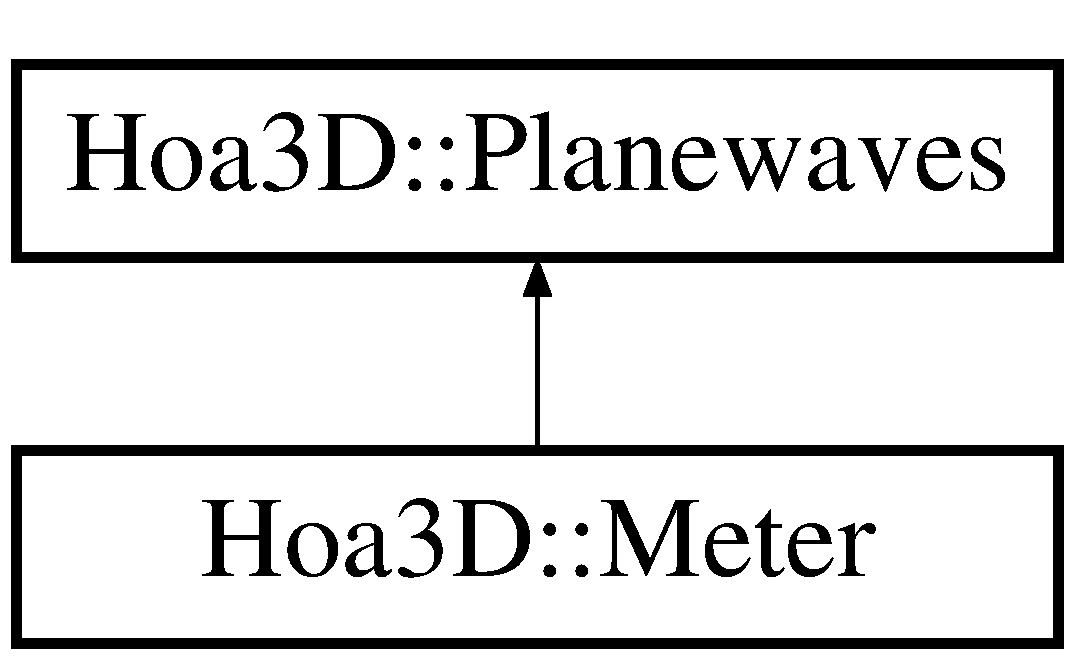
\includegraphics[height=2.000000cm]{class_hoa3_d_1_1_meter}
\end{center}
\end{figure}
\subsection*{Public Member Functions}
\begin{DoxyCompactItemize}
\item 
\hyperlink{class_hoa3_d_1_1_meter_a8dbe4a3655161c329540557cfed8c52a}{Meter} (unsigned int number\-Of\-Channels)
\begin{DoxyCompactList}\small\item\em The \hyperlink{class_hoa3_d_1_1_meter}{Meter} constructor. \end{DoxyCompactList}\item 
\hyperlink{class_hoa3_d_1_1_meter_a2f4d18e0007e96c1cd60e2f17d9575cc}{$\sim$\-Meter} ()
\begin{DoxyCompactList}\small\item\em The \hyperlink{class_hoa3_d_1_1_meter}{Meter} destructor. \end{DoxyCompactList}\item 
void \hyperlink{class_hoa3_d_1_1_meter_a85c538e8cf9791674a9ac6e602463dd0}{process} (const float $\ast$inputs)
\begin{DoxyCompactList}\small\item\em This method performs the widening with single precision. \end{DoxyCompactList}\item 
void \hyperlink{class_hoa3_d_1_1_meter_a273685843e1059b74b6d386dfb19c53b}{process} (const double $\ast$inputs)
\begin{DoxyCompactList}\small\item\em This method performs the widening with double precision. \end{DoxyCompactList}\end{DoxyCompactItemize}


\subsection{Detailed Description}
The ambisonic \hyperlink{class_hoa3_d_1_1_meter}{Meter}. 

The \hyperlink{class_hoa3_d_1_1_meter}{Meter} should be used to widen the sound propagation. 

Definition at line 17 of file Meter.\-h.



\subsection{Constructor \& Destructor Documentation}
\hypertarget{class_hoa3_d_1_1_meter_a8dbe4a3655161c329540557cfed8c52a}{\index{Hoa3\-D\-::\-Meter@{Hoa3\-D\-::\-Meter}!Meter@{Meter}}
\index{Meter@{Meter}!Hoa3D::Meter@{Hoa3\-D\-::\-Meter}}
\subsubsection[{Meter}]{\setlength{\rightskip}{0pt plus 5cm}Hoa3\-D\-::\-Meter\-::\-Meter (
\begin{DoxyParamCaption}
\item[{unsigned int}]{number\-Of\-Channels}
\end{DoxyParamCaption}
)}}\label{class_hoa3_d_1_1_meter_a8dbe4a3655161c329540557cfed8c52a}


The \hyperlink{class_hoa3_d_1_1_meter}{Meter} constructor. 

The \hyperlink{class_hoa3_d_1_1_meter}{Meter} constructor allocates and initialize the member values to computes spherical harmonics weighted coefficients depending of a decomposition order. The order must be at least 1.


\begin{DoxyParams}{Parameters}
{\em order} & The order. \\
\hline
\end{DoxyParams}


Definition at line 11 of file Meter.\-cpp.

\hypertarget{class_hoa3_d_1_1_meter_a2f4d18e0007e96c1cd60e2f17d9575cc}{\index{Hoa3\-D\-::\-Meter@{Hoa3\-D\-::\-Meter}!$\sim$\-Meter@{$\sim$\-Meter}}
\index{$\sim$\-Meter@{$\sim$\-Meter}!Hoa3D::Meter@{Hoa3\-D\-::\-Meter}}
\subsubsection[{$\sim$\-Meter}]{\setlength{\rightskip}{0pt plus 5cm}Hoa3\-D\-::\-Meter\-::$\sim$\-Meter (
\begin{DoxyParamCaption}
{}
\end{DoxyParamCaption}
)}}\label{class_hoa3_d_1_1_meter_a2f4d18e0007e96c1cd60e2f17d9575cc}


The \hyperlink{class_hoa3_d_1_1_meter}{Meter} destructor. 

The \hyperlink{class_hoa3_d_1_1_meter}{Meter} destructor free the memory. 

Definition at line 24 of file Meter.\-cpp.



\subsection{Member Function Documentation}
\hypertarget{class_hoa3_d_1_1_meter_a85c538e8cf9791674a9ac6e602463dd0}{\index{Hoa3\-D\-::\-Meter@{Hoa3\-D\-::\-Meter}!process@{process}}
\index{process@{process}!Hoa3D::Meter@{Hoa3\-D\-::\-Meter}}
\subsubsection[{process}]{\setlength{\rightskip}{0pt plus 5cm}void Hoa3\-D\-::\-Meter\-::process (
\begin{DoxyParamCaption}
\item[{const float $\ast$}]{inputs}
\end{DoxyParamCaption}
)}}\label{class_hoa3_d_1_1_meter_a85c538e8cf9791674a9ac6e602463dd0}


This method performs the widening with single precision. 

You should use this method for in-\/place or not-\/in-\/place processing and performs the widening sample by sample. The inputs array and outputs array contains the spherical harmonics samples and the minimum size must be the number of harmonics.


\begin{DoxyParams}{Parameters}
{\em inputs} & The input array. \\
\hline
\end{DoxyParams}


Definition at line 16 of file Meter.\-cpp.

\hypertarget{class_hoa3_d_1_1_meter_a273685843e1059b74b6d386dfb19c53b}{\index{Hoa3\-D\-::\-Meter@{Hoa3\-D\-::\-Meter}!process@{process}}
\index{process@{process}!Hoa3D::Meter@{Hoa3\-D\-::\-Meter}}
\subsubsection[{process}]{\setlength{\rightskip}{0pt plus 5cm}void Hoa3\-D\-::\-Meter\-::process (
\begin{DoxyParamCaption}
\item[{const double $\ast$}]{inputs}
\end{DoxyParamCaption}
)}}\label{class_hoa3_d_1_1_meter_a273685843e1059b74b6d386dfb19c53b}


This method performs the widening with double precision. 

You should use this method for in-\/place or not-\/in-\/place processing and performs the widening sample by sample. The inputs array and outputs array contains the spherical harmonics samples and the minimum size must be the number of harmonics.


\begin{DoxyParams}{Parameters}
{\em inputs} & The input array. \\
\hline
\end{DoxyParams}


Definition at line 20 of file Meter.\-cpp.



The documentation for this class was generated from the following files\-:\begin{DoxyCompactItemize}
\item 
/\-Users/\-Pierre/\-Source\-Tree/\-Hoa\-Library/\-Sources/\-Hoa3\-D/Meter.\-h\item 
/\-Users/\-Pierre/\-Source\-Tree/\-Hoa\-Library/\-Sources/\-Hoa3\-D/Meter.\-cpp\end{DoxyCompactItemize}

\hypertarget{class_hoa2_d_1_1_optim}{\section{Hoa2\-D\-:\-:Optim Class Reference}
\label{class_hoa2_d_1_1_optim}\index{Hoa2\-D\-::\-Optim@{Hoa2\-D\-::\-Optim}}
}


The ambisonic optimization.  




{\ttfamily \#include $<$Optim.\-h$>$}

Inheritance diagram for Hoa2\-D\-:\-:Optim\-:\begin{figure}[H]
\begin{center}
\leavevmode
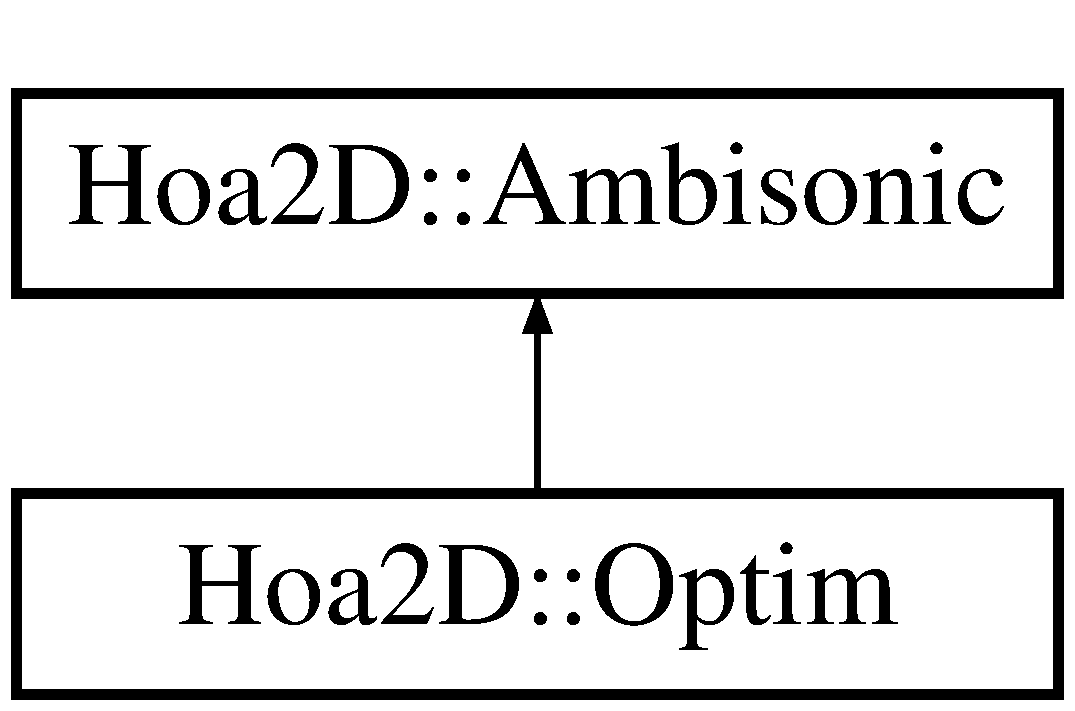
\includegraphics[height=2.000000cm]{class_hoa2_d_1_1_optim}
\end{center}
\end{figure}
\subsection*{Public Types}
\begin{DoxyCompactItemize}
\item 
enum \hyperlink{class_hoa2_d_1_1_optim_ae40f22368cb55699cf19729e37c0aff3}{Mode} \{ \hyperlink{class_hoa2_d_1_1_optim_ae40f22368cb55699cf19729e37c0aff3af5bbb98a42968855f2f43d9a708ae8d2}{Basic} = 0, 
\hyperlink{class_hoa2_d_1_1_optim_ae40f22368cb55699cf19729e37c0aff3a6b8b2446e2cffae18f5f4625b68e0f21}{Max\-Re} = 1, 
\hyperlink{class_hoa2_d_1_1_optim_ae40f22368cb55699cf19729e37c0aff3aa9a64070fdf166180add5ac7a8e24567}{In\-Phase} = 2
 \}
\end{DoxyCompactItemize}
\subsection*{Public Member Functions}
\begin{DoxyCompactItemize}
\item 
\hyperlink{class_hoa2_d_1_1_optim_a5e11da74b3e87ad15db6538d31eb3628}{Optim} (unsigned int order, \hyperlink{class_hoa2_d_1_1_optim_ae40f22368cb55699cf19729e37c0aff3}{Mode} mode)
\begin{DoxyCompactList}\small\item\em The optimization constructor. \end{DoxyCompactList}\item 
\hyperlink{class_hoa2_d_1_1_optim_a71b6d88873b054944db6efd2713bf8d3}{$\sim$\-Optim} ()
\begin{DoxyCompactList}\small\item\em The optimization destructor. \end{DoxyCompactList}\item 
\hyperlink{class_hoa2_d_1_1_optim_ae40f22368cb55699cf19729e37c0aff3}{Mode} \hyperlink{class_hoa2_d_1_1_optim_ab75c7150c5918ed05219212b426aa04b}{get\-Mode} () const 
\begin{DoxyCompactList}\small\item\em Retrieve the optimization mode. \end{DoxyCompactList}\item 
void \hyperlink{class_hoa2_d_1_1_optim_a2ea2227817c133aeaf2732880d8214ce}{set\-Mode} (\hyperlink{class_hoa2_d_1_1_optim_ae40f22368cb55699cf19729e37c0aff3}{Mode} mode)
\begin{DoxyCompactList}\small\item\em This method set the optimization mode. \end{DoxyCompactList}\item 
void \hyperlink{class_hoa2_d_1_1_optim_afca15242cbca4fefe08c6f17d2b42241}{process} (const float $\ast$inputs, float $\ast$outputs)
\begin{DoxyCompactList}\small\item\em This method performs the optimization with single precision. \end{DoxyCompactList}\item 
void \hyperlink{class_hoa2_d_1_1_optim_ac0c905a79204c921568952c787376120}{process} (const double $\ast$inputs, double $\ast$outputs)
\begin{DoxyCompactList}\small\item\em This method performs the optimization with double precision. \end{DoxyCompactList}\end{DoxyCompactItemize}


\subsection{Detailed Description}
The ambisonic optimization. 

The optimization should be used to optimize the ambisonic sound field. There are 3 optimization modes, Basic (no optimization), Max\-Re (energy vector optimization) and In\-Phase (energy and velocity vector optimization). Basic has no effect, it should be used with a perfect ambisonic loudspeakers, arrengement where all the loudspeakers are to equal distance on a circle, and for a listener placed at the perfect center of the circle. Max\-Re should be used for auditory confined to the center of the circle. In\-Phase should be used when the auditory covers the entire loudspeakers area and when the loudspeakers arragement is not a perfect circle or when the loudspeakers are not to equal distance. Note that the optimizations decrease the precision of the sound field restitution thus it can be compared to particular cases of the fractional orders. 

Definition at line 16 of file Optim.\-h.



\subsection{Member Enumeration Documentation}
\hypertarget{class_hoa2_d_1_1_optim_ae40f22368cb55699cf19729e37c0aff3}{\index{Hoa2\-D\-::\-Optim@{Hoa2\-D\-::\-Optim}!Mode@{Mode}}
\index{Mode@{Mode}!Hoa2D::Optim@{Hoa2\-D\-::\-Optim}}
\subsubsection[{Mode}]{\setlength{\rightskip}{0pt plus 5cm}enum {\bf Hoa2\-D\-::\-Optim\-::\-Mode}}}\label{class_hoa2_d_1_1_optim_ae40f22368cb55699cf19729e37c0aff3}
\begin{Desc}
\item[Enumerator]\par
\begin{description}
\index{Basic@{Basic}!Hoa2\-D\-::\-Optim@{Hoa2\-D\-::\-Optim}}\index{Hoa2\-D\-::\-Optim@{Hoa2\-D\-::\-Optim}!Basic@{Basic}}\item[{\em 
\hypertarget{class_hoa2_d_1_1_optim_ae40f22368cb55699cf19729e37c0aff3af5bbb98a42968855f2f43d9a708ae8d2}{Basic}\label{class_hoa2_d_1_1_optim_ae40f22368cb55699cf19729e37c0aff3af5bbb98a42968855f2f43d9a708ae8d2}
}]Basic Optimization \index{Max\-Re@{Max\-Re}!Hoa2\-D\-::\-Optim@{Hoa2\-D\-::\-Optim}}\index{Hoa2\-D\-::\-Optim@{Hoa2\-D\-::\-Optim}!Max\-Re@{Max\-Re}}\item[{\em 
\hypertarget{class_hoa2_d_1_1_optim_ae40f22368cb55699cf19729e37c0aff3a6b8b2446e2cffae18f5f4625b68e0f21}{Max\-Re}\label{class_hoa2_d_1_1_optim_ae40f22368cb55699cf19729e37c0aff3a6b8b2446e2cffae18f5f4625b68e0f21}
}]Max Re Optimization \index{In\-Phase@{In\-Phase}!Hoa2\-D\-::\-Optim@{Hoa2\-D\-::\-Optim}}\index{Hoa2\-D\-::\-Optim@{Hoa2\-D\-::\-Optim}!In\-Phase@{In\-Phase}}\item[{\em 
\hypertarget{class_hoa2_d_1_1_optim_ae40f22368cb55699cf19729e37c0aff3aa9a64070fdf166180add5ac7a8e24567}{In\-Phase}\label{class_hoa2_d_1_1_optim_ae40f22368cb55699cf19729e37c0aff3aa9a64070fdf166180add5ac7a8e24567}
}]In Phase Optimization \end{description}
\end{Desc}


Definition at line 19 of file Optim.\-h.



\subsection{Constructor \& Destructor Documentation}
\hypertarget{class_hoa2_d_1_1_optim_a5e11da74b3e87ad15db6538d31eb3628}{\index{Hoa2\-D\-::\-Optim@{Hoa2\-D\-::\-Optim}!Optim@{Optim}}
\index{Optim@{Optim}!Hoa2D::Optim@{Hoa2\-D\-::\-Optim}}
\subsubsection[{Optim}]{\setlength{\rightskip}{0pt plus 5cm}Hoa2\-D\-::\-Optim\-::\-Optim (
\begin{DoxyParamCaption}
\item[{unsigned int}]{order, }
\item[{{\bf Mode}}]{mode}
\end{DoxyParamCaption}
)}}\label{class_hoa2_d_1_1_optim_a5e11da74b3e87ad15db6538d31eb3628}


The optimization constructor. 

The optimization constructor allocates and initialize the member values to computes spherical harmonics weighted coefficients depending of a decomposition order. The order must be at least 1.


\begin{DoxyParams}{Parameters}
{\em order} & The order. \\
\hline
\end{DoxyParams}


Definition at line 11 of file Optim.\-cpp.

\hypertarget{class_hoa2_d_1_1_optim_a71b6d88873b054944db6efd2713bf8d3}{\index{Hoa2\-D\-::\-Optim@{Hoa2\-D\-::\-Optim}!$\sim$\-Optim@{$\sim$\-Optim}}
\index{$\sim$\-Optim@{$\sim$\-Optim}!Hoa2D::Optim@{Hoa2\-D\-::\-Optim}}
\subsubsection[{$\sim$\-Optim}]{\setlength{\rightskip}{0pt plus 5cm}Hoa2\-D\-::\-Optim\-::$\sim$\-Optim (
\begin{DoxyParamCaption}
{}
\end{DoxyParamCaption}
)}}\label{class_hoa2_d_1_1_optim_a71b6d88873b054944db6efd2713bf8d3}


The optimization destructor. 

The optimization destructor free the memory. 

Definition at line 59 of file Optim.\-cpp.



\subsection{Member Function Documentation}
\hypertarget{class_hoa2_d_1_1_optim_ab75c7150c5918ed05219212b426aa04b}{\index{Hoa2\-D\-::\-Optim@{Hoa2\-D\-::\-Optim}!get\-Mode@{get\-Mode}}
\index{get\-Mode@{get\-Mode}!Hoa2D::Optim@{Hoa2\-D\-::\-Optim}}
\subsubsection[{get\-Mode}]{\setlength{\rightskip}{0pt plus 5cm}{\bf Mode} Hoa2\-D\-::\-Optim\-::get\-Mode (
\begin{DoxyParamCaption}
{}
\end{DoxyParamCaption}
) const\hspace{0.3cm}{\ttfamily [inline]}}}\label{class_hoa2_d_1_1_optim_ab75c7150c5918ed05219212b426aa04b}


Retrieve the optimization mode. 

Retrieve the optimization mode \-: Basic, Max\-Re or In\-Phase.

\begin{DoxyReturn}{Returns}
The method returns the optimization mode. 
\end{DoxyReturn}


Definition at line 50 of file Optim.\-h.

\hypertarget{class_hoa2_d_1_1_optim_afca15242cbca4fefe08c6f17d2b42241}{\index{Hoa2\-D\-::\-Optim@{Hoa2\-D\-::\-Optim}!process@{process}}
\index{process@{process}!Hoa2D::Optim@{Hoa2\-D\-::\-Optim}}
\subsubsection[{process}]{\setlength{\rightskip}{0pt plus 5cm}void Hoa2\-D\-::\-Optim\-::process (
\begin{DoxyParamCaption}
\item[{const float $\ast$}]{inputs, }
\item[{float $\ast$}]{outputs}
\end{DoxyParamCaption}
)}}\label{class_hoa2_d_1_1_optim_afca15242cbca4fefe08c6f17d2b42241}


This method performs the optimization with single precision. 

You should use this method for in-\/place or not-\/in-\/place processing and performs the optimization sample by sample. The inputs array and outputs array contains the spherical harmonics samples and the minimum size must be the number of harmonics.


\begin{DoxyParams}{Parameters}
{\em inputs} & The inputs array. \\
\hline
{\em outputs} & The outputs array. \\
\hline
\end{DoxyParams}


Definition at line 47 of file Optim.\-cpp.

\hypertarget{class_hoa2_d_1_1_optim_ac0c905a79204c921568952c787376120}{\index{Hoa2\-D\-::\-Optim@{Hoa2\-D\-::\-Optim}!process@{process}}
\index{process@{process}!Hoa2D::Optim@{Hoa2\-D\-::\-Optim}}
\subsubsection[{process}]{\setlength{\rightskip}{0pt plus 5cm}void Hoa2\-D\-::\-Optim\-::process (
\begin{DoxyParamCaption}
\item[{const double $\ast$}]{inputs, }
\item[{double $\ast$}]{outputs}
\end{DoxyParamCaption}
)}}\label{class_hoa2_d_1_1_optim_ac0c905a79204c921568952c787376120}


This method performs the optimization with double precision. 

You should use this method for in-\/place or not-\/in-\/place processing and performs the optimization sample by sample. The inputs array and outputs array contains the spherical harmonics samples and the minimum size must be the number of harmonics.


\begin{DoxyParams}{Parameters}
{\em inputs} & The inputs array. \\
\hline
{\em outputs} & The outputs array. \\
\hline
\end{DoxyParams}


Definition at line 53 of file Optim.\-cpp.

\hypertarget{class_hoa2_d_1_1_optim_a2ea2227817c133aeaf2732880d8214ce}{\index{Hoa2\-D\-::\-Optim@{Hoa2\-D\-::\-Optim}!set\-Mode@{set\-Mode}}
\index{set\-Mode@{set\-Mode}!Hoa2D::Optim@{Hoa2\-D\-::\-Optim}}
\subsubsection[{set\-Mode}]{\setlength{\rightskip}{0pt plus 5cm}void Hoa2\-D\-::\-Optim\-::set\-Mode (
\begin{DoxyParamCaption}
\item[{{\bf Mode}}]{mode}
\end{DoxyParamCaption}
)}}\label{class_hoa2_d_1_1_optim_a2ea2227817c133aeaf2732880d8214ce}


This method set the optimization mode. 

The mode should be one of the 3 optimization modes, Basic, Max\-Re or In\-Phase.


\begin{DoxyParams}{Parameters}
{\em mode} & The optimization mode. \\
\hline
\end{DoxyParams}


Definition at line 17 of file Optim.\-cpp.



The documentation for this class was generated from the following files\-:\begin{DoxyCompactItemize}
\item 
/\-Users/\-Pierre/\-Source\-Tree/\-Hoa\-Library/\-Sources/\-Hoa2\-D/Optim.\-h\item 
/\-Users/\-Pierre/\-Source\-Tree/\-Hoa\-Library/\-Sources/\-Hoa2\-D/Optim.\-cpp\end{DoxyCompactItemize}

\hypertarget{class_hoa3_d_1_1_optim}{\section{Hoa3\-D\-:\-:Optim Class Reference}
\label{class_hoa3_d_1_1_optim}\index{Hoa3\-D\-::\-Optim@{Hoa3\-D\-::\-Optim}}
}


The ambisonic optimization.  




{\ttfamily \#include $<$Optim.\-h$>$}

Inheritance diagram for Hoa3\-D\-:\-:Optim\-:\begin{figure}[H]
\begin{center}
\leavevmode
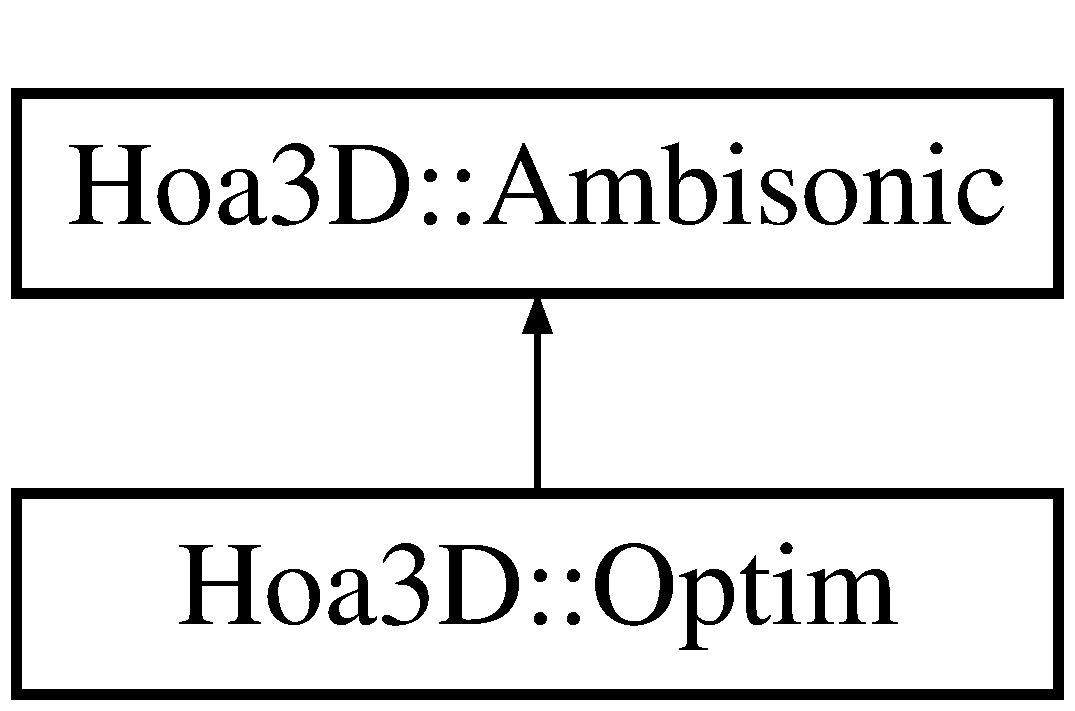
\includegraphics[height=2.000000cm]{class_hoa3_d_1_1_optim}
\end{center}
\end{figure}
\subsection*{Public Types}
\begin{DoxyCompactItemize}
\item 
enum \hyperlink{class_hoa3_d_1_1_optim_a1a153ac21e7a112279824f17981cf147}{Mode} \{ \hyperlink{class_hoa3_d_1_1_optim_a1a153ac21e7a112279824f17981cf147a89acb58975922396713cc88cafc55b45}{Basic} = 0, 
\hyperlink{class_hoa3_d_1_1_optim_a1a153ac21e7a112279824f17981cf147a491a405ba48de3977668d54a8d9ff44a}{Max\-Re} = 1, 
\hyperlink{class_hoa3_d_1_1_optim_a1a153ac21e7a112279824f17981cf147a55da4ad4519ee8860e9ea45cc475241c}{In\-Phase} = 2
 \}
\end{DoxyCompactItemize}
\subsection*{Public Member Functions}
\begin{DoxyCompactItemize}
\item 
\hyperlink{class_hoa3_d_1_1_optim_ab53ffe61910a75637afafb7f4f3ba788}{Optim} (unsigned int order, \hyperlink{class_hoa3_d_1_1_optim_a1a153ac21e7a112279824f17981cf147}{Mode} mode)
\begin{DoxyCompactList}\small\item\em The optimization constructor. \end{DoxyCompactList}\item 
\hyperlink{class_hoa3_d_1_1_optim_a11c05a8b458f79ba09f4eefad63e0b20}{$\sim$\-Optim} ()
\begin{DoxyCompactList}\small\item\em The optimization destructor. \end{DoxyCompactList}\item 
void \hyperlink{class_hoa3_d_1_1_optim_abb49c9e6a327bc62ac6491cd3046a10a}{set\-Mode} (\hyperlink{class_hoa3_d_1_1_optim_a1a153ac21e7a112279824f17981cf147}{Mode} mode)
\begin{DoxyCompactList}\small\item\em This method set the optimization mode. \end{DoxyCompactList}\item 
\hyperlink{class_hoa3_d_1_1_optim_a1a153ac21e7a112279824f17981cf147}{Mode} \hyperlink{class_hoa3_d_1_1_optim_a0446c68d06a5fd112f3e608c82d69b7f}{get\-Mode} () const 
\begin{DoxyCompactList}\small\item\em Retrieve the optimization mode. \end{DoxyCompactList}\item 
void \hyperlink{class_hoa3_d_1_1_optim_a13f8cb746e5bcc3c096bd0c0bf1a6435}{process} (const float $\ast$inputs, float $\ast$outputs)
\begin{DoxyCompactList}\small\item\em This method performs the optimization with single precision. \end{DoxyCompactList}\item 
void \hyperlink{class_hoa3_d_1_1_optim_a6c2e7ce20ec5f98e9e609040144ea99d}{process} (const double $\ast$inputs, double $\ast$outputs)
\begin{DoxyCompactList}\small\item\em This method performs the optimization with double precision. \end{DoxyCompactList}\end{DoxyCompactItemize}


\subsection{Detailed Description}
The ambisonic optimization. 

The optimization should be used to optimize the ambisonic sound field. There are 3 optimization modes, Basic (no optimizations), Max\-Re (energy vector optimization) and In\-Phase (energy and velocity vector optimization). Basic has no effect, it should be used with a perfect ambisonic loudspeakers (arrengement where all the loudspeakers are to equal distance on a sphere) and for a listener placed at the perfect center of the sphere. Max\-Re should be used for auditory confined to the center of the sphere. In\-Phase should be used when the auditory covers the entire loudspeaker area and when the loudspeakers arragement is not a perfect sphere or when the loudspeakers are not to equal distance. Note that the optimizations decrease the precision sound field restitution thus it can be compared to particular cases of the fractional orders. 

Definition at line 17 of file Optim.\-h.



\subsection{Member Enumeration Documentation}
\hypertarget{class_hoa3_d_1_1_optim_a1a153ac21e7a112279824f17981cf147}{\index{Hoa3\-D\-::\-Optim@{Hoa3\-D\-::\-Optim}!Mode@{Mode}}
\index{Mode@{Mode}!Hoa3D::Optim@{Hoa3\-D\-::\-Optim}}
\subsubsection[{Mode}]{\setlength{\rightskip}{0pt plus 5cm}enum {\bf Hoa3\-D\-::\-Optim\-::\-Mode}}}\label{class_hoa3_d_1_1_optim_a1a153ac21e7a112279824f17981cf147}
\begin{Desc}
\item[Enumerator]\par
\begin{description}
\index{Basic@{Basic}!Hoa3\-D\-::\-Optim@{Hoa3\-D\-::\-Optim}}\index{Hoa3\-D\-::\-Optim@{Hoa3\-D\-::\-Optim}!Basic@{Basic}}\item[{\em 
\hypertarget{class_hoa3_d_1_1_optim_a1a153ac21e7a112279824f17981cf147a89acb58975922396713cc88cafc55b45}{Basic}\label{class_hoa3_d_1_1_optim_a1a153ac21e7a112279824f17981cf147a89acb58975922396713cc88cafc55b45}
}]basic Optimization \index{Max\-Re@{Max\-Re}!Hoa3\-D\-::\-Optim@{Hoa3\-D\-::\-Optim}}\index{Hoa3\-D\-::\-Optim@{Hoa3\-D\-::\-Optim}!Max\-Re@{Max\-Re}}\item[{\em 
\hypertarget{class_hoa3_d_1_1_optim_a1a153ac21e7a112279824f17981cf147a491a405ba48de3977668d54a8d9ff44a}{Max\-Re}\label{class_hoa3_d_1_1_optim_a1a153ac21e7a112279824f17981cf147a491a405ba48de3977668d54a8d9ff44a}
}]max-\/re Optimization \index{In\-Phase@{In\-Phase}!Hoa3\-D\-::\-Optim@{Hoa3\-D\-::\-Optim}}\index{Hoa3\-D\-::\-Optim@{Hoa3\-D\-::\-Optim}!In\-Phase@{In\-Phase}}\item[{\em 
\hypertarget{class_hoa3_d_1_1_optim_a1a153ac21e7a112279824f17981cf147a55da4ad4519ee8860e9ea45cc475241c}{In\-Phase}\label{class_hoa3_d_1_1_optim_a1a153ac21e7a112279824f17981cf147a55da4ad4519ee8860e9ea45cc475241c}
}]in-\/phase Optimization \end{description}
\end{Desc}


Definition at line 20 of file Optim.\-h.



\subsection{Constructor \& Destructor Documentation}
\hypertarget{class_hoa3_d_1_1_optim_ab53ffe61910a75637afafb7f4f3ba788}{\index{Hoa3\-D\-::\-Optim@{Hoa3\-D\-::\-Optim}!Optim@{Optim}}
\index{Optim@{Optim}!Hoa3D::Optim@{Hoa3\-D\-::\-Optim}}
\subsubsection[{Optim}]{\setlength{\rightskip}{0pt plus 5cm}Hoa3\-D\-::\-Optim\-::\-Optim (
\begin{DoxyParamCaption}
\item[{unsigned int}]{order, }
\item[{{\bf Mode}}]{mode}
\end{DoxyParamCaption}
)}}\label{class_hoa3_d_1_1_optim_ab53ffe61910a75637afafb7f4f3ba788}


The optimization constructor. 

The optimization constructor allocates and initialize the member values to computes spherical harmonics weighted coefficients depending of a decomposition order. The order must be at least 1.


\begin{DoxyParams}{Parameters}
{\em order} & The order. \\
\hline
{\em mode} & The optimization mode. \\
\hline
\end{DoxyParams}


Definition at line 11 of file Optim.\-cpp.

\hypertarget{class_hoa3_d_1_1_optim_a11c05a8b458f79ba09f4eefad63e0b20}{\index{Hoa3\-D\-::\-Optim@{Hoa3\-D\-::\-Optim}!$\sim$\-Optim@{$\sim$\-Optim}}
\index{$\sim$\-Optim@{$\sim$\-Optim}!Hoa3D::Optim@{Hoa3\-D\-::\-Optim}}
\subsubsection[{$\sim$\-Optim}]{\setlength{\rightskip}{0pt plus 5cm}Hoa3\-D\-::\-Optim\-::$\sim$\-Optim (
\begin{DoxyParamCaption}
{}
\end{DoxyParamCaption}
)}}\label{class_hoa3_d_1_1_optim_a11c05a8b458f79ba09f4eefad63e0b20}


The optimization destructor. 

The optimization destructor free the memory. 

Definition at line 57 of file Optim.\-cpp.



\subsection{Member Function Documentation}
\hypertarget{class_hoa3_d_1_1_optim_a0446c68d06a5fd112f3e608c82d69b7f}{\index{Hoa3\-D\-::\-Optim@{Hoa3\-D\-::\-Optim}!get\-Mode@{get\-Mode}}
\index{get\-Mode@{get\-Mode}!Hoa3D::Optim@{Hoa3\-D\-::\-Optim}}
\subsubsection[{get\-Mode}]{\setlength{\rightskip}{0pt plus 5cm}{\bf Mode} Hoa3\-D\-::\-Optim\-::get\-Mode (
\begin{DoxyParamCaption}
{}
\end{DoxyParamCaption}
) const\hspace{0.3cm}{\ttfamily [inline]}}}\label{class_hoa3_d_1_1_optim_a0446c68d06a5fd112f3e608c82d69b7f}


Retrieve the optimization mode. 

Retrieve the optimization mode \-: Basic, Max\-Re or In\-Phase.

\begin{DoxyReturn}{Returns}
The method returns the optimization mode. 
\end{DoxyReturn}


Definition at line 59 of file Optim.\-h.

\hypertarget{class_hoa3_d_1_1_optim_a13f8cb746e5bcc3c096bd0c0bf1a6435}{\index{Hoa3\-D\-::\-Optim@{Hoa3\-D\-::\-Optim}!process@{process}}
\index{process@{process}!Hoa3D::Optim@{Hoa3\-D\-::\-Optim}}
\subsubsection[{process}]{\setlength{\rightskip}{0pt plus 5cm}void Hoa3\-D\-::\-Optim\-::process (
\begin{DoxyParamCaption}
\item[{const float $\ast$}]{inputs, }
\item[{float $\ast$}]{outputs}
\end{DoxyParamCaption}
)}}\label{class_hoa3_d_1_1_optim_a13f8cb746e5bcc3c096bd0c0bf1a6435}


This method performs the optimization with single precision. 

You should use this method for in-\/place or not-\/in-\/place processing and performs the optimization sample by sample. The inputs array and outputs array contains the spherical harmonics samples and the minimum size must be the number of harmonics.


\begin{DoxyParams}{Parameters}
{\em inputs} & The input array. \\
\hline
{\em outputs} & The output array. \\
\hline
\end{DoxyParams}


Definition at line 45 of file Optim.\-cpp.

\hypertarget{class_hoa3_d_1_1_optim_a6c2e7ce20ec5f98e9e609040144ea99d}{\index{Hoa3\-D\-::\-Optim@{Hoa3\-D\-::\-Optim}!process@{process}}
\index{process@{process}!Hoa3D::Optim@{Hoa3\-D\-::\-Optim}}
\subsubsection[{process}]{\setlength{\rightskip}{0pt plus 5cm}void Hoa3\-D\-::\-Optim\-::process (
\begin{DoxyParamCaption}
\item[{const double $\ast$}]{inputs, }
\item[{double $\ast$}]{outputs}
\end{DoxyParamCaption}
)}}\label{class_hoa3_d_1_1_optim_a6c2e7ce20ec5f98e9e609040144ea99d}


This method performs the optimization with double precision. 

You should use this method for in-\/place or not-\/in-\/place processing and performs the optimization sample by sample. The inputs array and outputs array contains the spherical harmonics samples and the minimum size must be the number of harmonics.


\begin{DoxyParams}{Parameters}
{\em inputs} & The input array. \\
\hline
{\em outputs} & The output array. \\
\hline
\end{DoxyParams}


Definition at line 51 of file Optim.\-cpp.

\hypertarget{class_hoa3_d_1_1_optim_abb49c9e6a327bc62ac6491cd3046a10a}{\index{Hoa3\-D\-::\-Optim@{Hoa3\-D\-::\-Optim}!set\-Mode@{set\-Mode}}
\index{set\-Mode@{set\-Mode}!Hoa3D::Optim@{Hoa3\-D\-::\-Optim}}
\subsubsection[{set\-Mode}]{\setlength{\rightskip}{0pt plus 5cm}void Hoa3\-D\-::\-Optim\-::set\-Mode (
\begin{DoxyParamCaption}
\item[{{\bf Mode}}]{mode}
\end{DoxyParamCaption}
)}}\label{class_hoa3_d_1_1_optim_abb49c9e6a327bc62ac6491cd3046a10a}


This method set the optimization mode. 

The mode should be one of the 3 optimization modes, Basic, Max\-Re or In\-Phase.


\begin{DoxyParams}{Parameters}
{\em mode} & The optimization mode. \\
\hline
\end{DoxyParams}


Definition at line 17 of file Optim.\-cpp.



The documentation for this class was generated from the following files\-:\begin{DoxyCompactItemize}
\item 
/\-Users/\-Pierre/\-Source\-Tree/\-Hoa\-Library/\-Sources/\-Hoa3\-D/Optim.\-h\item 
/\-Users/\-Pierre/\-Source\-Tree/\-Hoa\-Library/\-Sources/\-Hoa3\-D/Optim.\-cpp\end{DoxyCompactItemize}

\hypertarget{class_hoa3_d_1_1_planewaves}{\section{Hoa3\-D\-:\-:Planewaves Class Reference}
\label{class_hoa3_d_1_1_planewaves}\index{Hoa3\-D\-::\-Planewaves@{Hoa3\-D\-::\-Planewaves}}
}


The planewaves class.  




{\ttfamily \#include $<$Planewaves.\-h$>$}

Inheritance diagram for Hoa3\-D\-:\-:Planewaves\-:\begin{figure}[H]
\begin{center}
\leavevmode
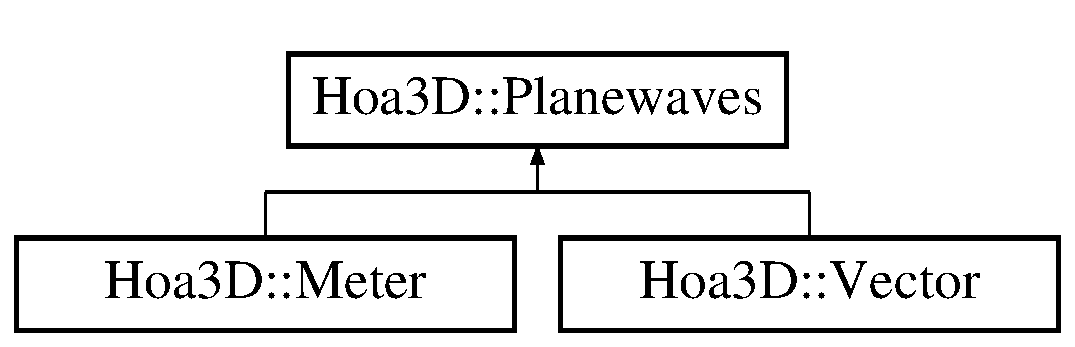
\includegraphics[height=2.000000cm]{class_hoa3_d_1_1_planewaves}
\end{center}
\end{figure}
\subsection*{Public Member Functions}
\begin{DoxyCompactItemize}
\item 
\hyperlink{class_hoa3_d_1_1_planewaves_ad190f41c56070493b4c55f4fcc9c6911}{Planewaves} (unsigned int number\-Of\-Loudspeakers)
\begin{DoxyCompactList}\small\item\em The planewaves constructor. \end{DoxyCompactList}\item 
\hyperlink{class_hoa3_d_1_1_planewaves_a51d3ba8bcdb8ad2e0c41e780f3c35d51}{$\sim$\-Planewaves} ()
\begin{DoxyCompactList}\small\item\em The planewaves destructor. \end{DoxyCompactList}\item 
void \hyperlink{class_hoa3_d_1_1_planewaves_ab39d630c1c191963cd35dd3b6a28ebc8}{set\-Loudspeaker\-Position} (unsigned int index, double azimuth, double elevation)
\begin{DoxyCompactList}\small\item\em Set the position of a loudspeaker. \end{DoxyCompactList}\item 
unsigned int \hyperlink{class_hoa3_d_1_1_planewaves_a467cdb1f079bb299225a9fac56a500e4}{get\-Number\-Of\-Loudspeakers} () const 
\begin{DoxyCompactList}\small\item\em Retrieve the number of loudspeakers. \end{DoxyCompactList}\item 
double \hyperlink{class_hoa3_d_1_1_planewaves_a8c0385dcf84e93ea035a91659122ce58}{get\-Loudspeaker\-Azimuth} (unsigned int index) const 
\begin{DoxyCompactList}\small\item\em Retrieve the azimuth of a loudspeaker. \end{DoxyCompactList}\item 
double \hyperlink{class_hoa3_d_1_1_planewaves_ae3b79c947e1923c5aad5067f7a2b29eb}{get\-Loudspeaker\-Elevation} (unsigned int index) const 
\begin{DoxyCompactList}\small\item\em Retrieve the elevation of a loudspeaker. \end{DoxyCompactList}\item 
double \hyperlink{class_hoa3_d_1_1_planewaves_ab88859d14af87a2766bcdb58f7d38b1c}{get\-Loudspeaker\-Abscissa} (unsigned int index) const 
\begin{DoxyCompactList}\small\item\em Retrieve the abscissa of a loudspeaker. \end{DoxyCompactList}\item 
double \hyperlink{class_hoa3_d_1_1_planewaves_a7bf08e3daaf9f9b1f66f5b8c7bde740f}{get\-Loudspeaker\-Ordinate} (unsigned int index) const 
\begin{DoxyCompactList}\small\item\em Retrieve the ordinate of a loudspeaker. \end{DoxyCompactList}\item 
double \hyperlink{class_hoa3_d_1_1_planewaves_acd3a7ad77d19ca916ecd8341bcf2c059}{get\-Loudspeaker\-Height} (unsigned int index) const 
\begin{DoxyCompactList}\small\item\em Retrieve the height of a loudspeaker. \end{DoxyCompactList}\item 
std\-::string \hyperlink{class_hoa3_d_1_1_planewaves_a264f20721feb71dd520a3ca115bfb141}{get\-Loudspeaker\-Name} (unsigned int index)
\begin{DoxyCompactList}\small\item\em Retrieve the number of loudspeaker. \end{DoxyCompactList}\end{DoxyCompactItemize}


\subsection{Detailed Description}
The planewaves class. 

The planewaves classes, that process on a set of loudspeakers, inherit from this class. It store basic informations like the number, the coordinates and the names of loudspeakers. 

Definition at line 19 of file Planewaves.\-h.



\subsection{Constructor \& Destructor Documentation}
\hypertarget{class_hoa3_d_1_1_planewaves_ad190f41c56070493b4c55f4fcc9c6911}{\index{Hoa3\-D\-::\-Planewaves@{Hoa3\-D\-::\-Planewaves}!Planewaves@{Planewaves}}
\index{Planewaves@{Planewaves}!Hoa3D::Planewaves@{Hoa3\-D\-::\-Planewaves}}
\subsubsection[{Planewaves}]{\setlength{\rightskip}{0pt plus 5cm}Hoa3\-D\-::\-Planewaves\-::\-Planewaves (
\begin{DoxyParamCaption}
\item[{unsigned int}]{number\-Of\-Loudspeakers}
\end{DoxyParamCaption}
)}}\label{class_hoa3_d_1_1_planewaves_ad190f41c56070493b4c55f4fcc9c6911}


The planewaves constructor. 

The lanewaves constructor allocates and initializes the general member values depending on a number of loudspeakers. The number of loudspkeakers must a least 1.


\begin{DoxyParams}{Parameters}
{\em number\-Of\-Loudspeakers} & The number of loudspeakers. \\
\hline
\end{DoxyParams}


Definition at line 11 of file Planewaves.\-cpp.

\hypertarget{class_hoa3_d_1_1_planewaves_a51d3ba8bcdb8ad2e0c41e780f3c35d51}{\index{Hoa3\-D\-::\-Planewaves@{Hoa3\-D\-::\-Planewaves}!$\sim$\-Planewaves@{$\sim$\-Planewaves}}
\index{$\sim$\-Planewaves@{$\sim$\-Planewaves}!Hoa3D::Planewaves@{Hoa3\-D\-::\-Planewaves}}
\subsubsection[{$\sim$\-Planewaves}]{\setlength{\rightskip}{0pt plus 5cm}Hoa3\-D\-::\-Planewaves\-::$\sim$\-Planewaves (
\begin{DoxyParamCaption}
{}
\end{DoxyParamCaption}
)}}\label{class_hoa3_d_1_1_planewaves_a51d3ba8bcdb8ad2e0c41e780f3c35d51}


The planewaves destructor. 

The \hyperlink{class_hoa3_d_1_1_planewaves}{Planewaves} destructor free the memorie allocated. 

Definition at line 26 of file Planewaves.\-cpp.



\subsection{Member Function Documentation}
\hypertarget{class_hoa3_d_1_1_planewaves_ab88859d14af87a2766bcdb58f7d38b1c}{\index{Hoa3\-D\-::\-Planewaves@{Hoa3\-D\-::\-Planewaves}!get\-Loudspeaker\-Abscissa@{get\-Loudspeaker\-Abscissa}}
\index{get\-Loudspeaker\-Abscissa@{get\-Loudspeaker\-Abscissa}!Hoa3D::Planewaves@{Hoa3\-D\-::\-Planewaves}}
\subsubsection[{get\-Loudspeaker\-Abscissa}]{\setlength{\rightskip}{0pt plus 5cm}double Hoa3\-D\-::\-Planewaves\-::get\-Loudspeaker\-Abscissa (
\begin{DoxyParamCaption}
\item[{unsigned int}]{index}
\end{DoxyParamCaption}
) const\hspace{0.3cm}{\ttfamily [inline]}}}\label{class_hoa3_d_1_1_planewaves_ab88859d14af87a2766bcdb58f7d38b1c}


Retrieve the abscissa of a loudspeaker. 

Retrieve the abscissa of a loudspeaker. The abscissa is between -\/1 and 1, -\/1 is the left of the soundfield, 0 is the center of the soundfield and 1 is the right of the soundfield. The maximum index must be the number of loudspeakers -\/ 1.


\begin{DoxyParams}{Parameters}
{\em index} & The index of the loudspeaker. \\
\hline
\end{DoxyParams}
\begin{DoxyReturn}{Returns}
The abscissa of the loudspeaker. 
\end{DoxyReturn}
\begin{DoxySeeAlso}{See Also}
\hyperlink{class_hoa3_d_1_1_planewaves_a7bf08e3daaf9f9b1f66f5b8c7bde740f}{get\-Loudspeaker\-Ordinate} 

\hyperlink{class_hoa3_d_1_1_planewaves_acd3a7ad77d19ca916ecd8341bcf2c059}{get\-Loudspeaker\-Height} 
\end{DoxySeeAlso}


Definition at line 91 of file Planewaves.\-h.

\hypertarget{class_hoa3_d_1_1_planewaves_a8c0385dcf84e93ea035a91659122ce58}{\index{Hoa3\-D\-::\-Planewaves@{Hoa3\-D\-::\-Planewaves}!get\-Loudspeaker\-Azimuth@{get\-Loudspeaker\-Azimuth}}
\index{get\-Loudspeaker\-Azimuth@{get\-Loudspeaker\-Azimuth}!Hoa3D::Planewaves@{Hoa3\-D\-::\-Planewaves}}
\subsubsection[{get\-Loudspeaker\-Azimuth}]{\setlength{\rightskip}{0pt plus 5cm}double Hoa3\-D\-::\-Planewaves\-::get\-Loudspeaker\-Azimuth (
\begin{DoxyParamCaption}
\item[{unsigned int}]{index}
\end{DoxyParamCaption}
) const\hspace{0.3cm}{\ttfamily [inline]}}}\label{class_hoa3_d_1_1_planewaves_a8c0385dcf84e93ea035a91659122ce58}


Retrieve the azimuth of a loudspeaker. 

Retrieve the azimuth of a loudspeaker. The azimuth of the loudspeaker is in radian, 0 radian is at the front of the soundfield and Pi is at the back of the sound field. The maximum index must be the number of loudspeakers -\/ 1.


\begin{DoxyParams}{Parameters}
{\em index} & The index of the loudspeaker. \\
\hline
\end{DoxyParams}
\begin{DoxyReturn}{Returns}
The azimuth of the loudspeaker. 
\end{DoxyReturn}
\begin{DoxySeeAlso}{See Also}
\hyperlink{class_hoa3_d_1_1_planewaves_ae3b79c947e1923c5aad5067f7a2b29eb}{get\-Loudspeaker\-Elevation} 
\end{DoxySeeAlso}


Definition at line 64 of file Planewaves.\-h.

\hypertarget{class_hoa3_d_1_1_planewaves_ae3b79c947e1923c5aad5067f7a2b29eb}{\index{Hoa3\-D\-::\-Planewaves@{Hoa3\-D\-::\-Planewaves}!get\-Loudspeaker\-Elevation@{get\-Loudspeaker\-Elevation}}
\index{get\-Loudspeaker\-Elevation@{get\-Loudspeaker\-Elevation}!Hoa3D::Planewaves@{Hoa3\-D\-::\-Planewaves}}
\subsubsection[{get\-Loudspeaker\-Elevation}]{\setlength{\rightskip}{0pt plus 5cm}double Hoa3\-D\-::\-Planewaves\-::get\-Loudspeaker\-Elevation (
\begin{DoxyParamCaption}
\item[{unsigned int}]{index}
\end{DoxyParamCaption}
) const\hspace{0.3cm}{\ttfamily [inline]}}}\label{class_hoa3_d_1_1_planewaves_ae3b79c947e1923c5aad5067f7a2b29eb}


Retrieve the elevation of a loudspeaker. 

Retrieve the elevation of a loudspeaker. The elevation is in radian between -\/1/2 Pi and 1/2 Pi, -\/1/2 Pi the the bottom of the sound field, 0 is the center of the sound field and 1/2 Pi is the top of the sound field. The maximum index must be the number of loudspeakers -\/ 1.


\begin{DoxyParams}{Parameters}
{\em index} & The index of the loudspeaker. \\
\hline
\end{DoxyParams}
\begin{DoxyReturn}{Returns}
The elevation of the loudspeaker. 
\end{DoxyReturn}
\begin{DoxySeeAlso}{See Also}
\hyperlink{class_hoa3_d_1_1_planewaves_a8c0385dcf84e93ea035a91659122ce58}{get\-Loudspeaker\-Azimuth} 
\end{DoxySeeAlso}


Definition at line 77 of file Planewaves.\-h.

\hypertarget{class_hoa3_d_1_1_planewaves_acd3a7ad77d19ca916ecd8341bcf2c059}{\index{Hoa3\-D\-::\-Planewaves@{Hoa3\-D\-::\-Planewaves}!get\-Loudspeaker\-Height@{get\-Loudspeaker\-Height}}
\index{get\-Loudspeaker\-Height@{get\-Loudspeaker\-Height}!Hoa3D::Planewaves@{Hoa3\-D\-::\-Planewaves}}
\subsubsection[{get\-Loudspeaker\-Height}]{\setlength{\rightskip}{0pt plus 5cm}double Hoa3\-D\-::\-Planewaves\-::get\-Loudspeaker\-Height (
\begin{DoxyParamCaption}
\item[{unsigned int}]{index}
\end{DoxyParamCaption}
) const\hspace{0.3cm}{\ttfamily [inline]}}}\label{class_hoa3_d_1_1_planewaves_acd3a7ad77d19ca916ecd8341bcf2c059}


Retrieve the height of a loudspeaker. 

Retrieve the height of a loudspeaker. The height is between -\/1 and 1, -\/1 is the bottom of the soundfield, 0 is the center of the soundfield and 1 is the top of the soundfield. The maximum index must be the number of loudspeakers -\/ 1.


\begin{DoxyParams}{Parameters}
{\em index} & The index of the loudspeaker. \\
\hline
\end{DoxyParams}
\begin{DoxyReturn}{Returns}
The height of the loudspeaker. 
\end{DoxyReturn}
\begin{DoxySeeAlso}{See Also}
\hyperlink{class_hoa3_d_1_1_planewaves_ab88859d14af87a2766bcdb58f7d38b1c}{get\-Loudspeaker\-Abscissa} 

\hyperlink{class_hoa3_d_1_1_planewaves_a7bf08e3daaf9f9b1f66f5b8c7bde740f}{get\-Loudspeaker\-Ordinate} 
\end{DoxySeeAlso}


Definition at line 119 of file Planewaves.\-h.

\hypertarget{class_hoa3_d_1_1_planewaves_a264f20721feb71dd520a3ca115bfb141}{\index{Hoa3\-D\-::\-Planewaves@{Hoa3\-D\-::\-Planewaves}!get\-Loudspeaker\-Name@{get\-Loudspeaker\-Name}}
\index{get\-Loudspeaker\-Name@{get\-Loudspeaker\-Name}!Hoa3D::Planewaves@{Hoa3\-D\-::\-Planewaves}}
\subsubsection[{get\-Loudspeaker\-Name}]{\setlength{\rightskip}{0pt plus 5cm}std\-::string Hoa3\-D\-::\-Planewaves\-::get\-Loudspeaker\-Name (
\begin{DoxyParamCaption}
\item[{unsigned int}]{index}
\end{DoxyParamCaption}
)\hspace{0.3cm}{\ttfamily [inline]}}}\label{class_hoa3_d_1_1_planewaves_a264f20721feb71dd520a3ca115bfb141}


Retrieve the number of loudspeaker. 

Retrieve a name for an loudspeaker in a std\-::string format that will be \char`\"{}\-Loudspeaker index azimuth elevation\char`\"{}.


\begin{DoxyParams}{Parameters}
{\em index} & The global index of a loudspeaker. \\
\hline
\end{DoxyParams}
\begin{DoxyReturn}{Returns}
The name of the loudspeaker 
\end{DoxyReturn}


Definition at line 131 of file Planewaves.\-h.

\hypertarget{class_hoa3_d_1_1_planewaves_a7bf08e3daaf9f9b1f66f5b8c7bde740f}{\index{Hoa3\-D\-::\-Planewaves@{Hoa3\-D\-::\-Planewaves}!get\-Loudspeaker\-Ordinate@{get\-Loudspeaker\-Ordinate}}
\index{get\-Loudspeaker\-Ordinate@{get\-Loudspeaker\-Ordinate}!Hoa3D::Planewaves@{Hoa3\-D\-::\-Planewaves}}
\subsubsection[{get\-Loudspeaker\-Ordinate}]{\setlength{\rightskip}{0pt plus 5cm}double Hoa3\-D\-::\-Planewaves\-::get\-Loudspeaker\-Ordinate (
\begin{DoxyParamCaption}
\item[{unsigned int}]{index}
\end{DoxyParamCaption}
) const\hspace{0.3cm}{\ttfamily [inline]}}}\label{class_hoa3_d_1_1_planewaves_a7bf08e3daaf9f9b1f66f5b8c7bde740f}


Retrieve the ordinate of a loudspeaker. 

Retrieve the ordinate of a loudspeaker. The ordinate is between -\/1 and 1, -\/1 is the back of the soundfield, 0 is the center of the soundfield and 1 is the front of the soundfield. The maximum index must be the number of loudspeakers -\/ 1.


\begin{DoxyParams}{Parameters}
{\em index} & The index of the loudspeaker. \\
\hline
\end{DoxyParams}
\begin{DoxyReturn}{Returns}
The ordinate of the loudspeaker. 
\end{DoxyReturn}
\begin{DoxySeeAlso}{See Also}
\hyperlink{class_hoa3_d_1_1_planewaves_ab88859d14af87a2766bcdb58f7d38b1c}{get\-Loudspeaker\-Abscissa} 

\hyperlink{class_hoa3_d_1_1_planewaves_acd3a7ad77d19ca916ecd8341bcf2c059}{get\-Loudspeaker\-Height} 
\end{DoxySeeAlso}


Definition at line 105 of file Planewaves.\-h.

\hypertarget{class_hoa3_d_1_1_planewaves_a467cdb1f079bb299225a9fac56a500e4}{\index{Hoa3\-D\-::\-Planewaves@{Hoa3\-D\-::\-Planewaves}!get\-Number\-Of\-Loudspeakers@{get\-Number\-Of\-Loudspeakers}}
\index{get\-Number\-Of\-Loudspeakers@{get\-Number\-Of\-Loudspeakers}!Hoa3D::Planewaves@{Hoa3\-D\-::\-Planewaves}}
\subsubsection[{get\-Number\-Of\-Loudspeakers}]{\setlength{\rightskip}{0pt plus 5cm}unsigned int Hoa3\-D\-::\-Planewaves\-::get\-Number\-Of\-Loudspeakers (
\begin{DoxyParamCaption}
{}
\end{DoxyParamCaption}
) const\hspace{0.3cm}{\ttfamily [inline]}}}\label{class_hoa3_d_1_1_planewaves_a467cdb1f079bb299225a9fac56a500e4}


Retrieve the number of loudspeakers. 

Retrieve the number of loudspeakers of the planewave class.

\begin{DoxyReturn}{Returns}
The number of loudspeakers. 
\end{DoxyReturn}


Definition at line 55 of file Planewaves.\-h.

\hypertarget{class_hoa3_d_1_1_planewaves_ab39d630c1c191963cd35dd3b6a28ebc8}{\index{Hoa3\-D\-::\-Planewaves@{Hoa3\-D\-::\-Planewaves}!set\-Loudspeaker\-Position@{set\-Loudspeaker\-Position}}
\index{set\-Loudspeaker\-Position@{set\-Loudspeaker\-Position}!Hoa3D::Planewaves@{Hoa3\-D\-::\-Planewaves}}
\subsubsection[{set\-Loudspeaker\-Position}]{\setlength{\rightskip}{0pt plus 5cm}void Hoa3\-D\-::\-Planewaves\-::set\-Loudspeaker\-Position (
\begin{DoxyParamCaption}
\item[{unsigned int}]{index, }
\item[{double}]{azimuth, }
\item[{double}]{elevation}
\end{DoxyParamCaption}
)}}\label{class_hoa3_d_1_1_planewaves_ab39d630c1c191963cd35dd3b6a28ebc8}


Set the position of a loudspeaker. 

Set the position of a loudspeaker with polar coordinates. The azimtuh is in radian between 0 and 2 Pi, O is the front of the soundfield and Pi is the back of the sound field. The elevation is in radian between -\/1/2 Pi and 1/2 Pi, -\/1/2 Pi the the bottom of the sound field, 0 is the center of the sound field and 1/2 Pi is the top of the sound field. The maximum index must be the number of loudspeakers -\/ 1.


\begin{DoxyParams}{Parameters}
{\em index} & The index of the loudspeaker. \\
\hline
{\em azimuth} & The azimuth. \\
\hline
{\em elevation} & The elevation. \\
\hline
\end{DoxyParams}


Definition at line 19 of file Planewaves.\-cpp.


\hypertarget{class_hoa2_d_1_1_rotate}{\section{Hoa2\-D\-:\-:Rotate Class Reference}
\label{class_hoa2_d_1_1_rotate}\index{Hoa2\-D\-::\-Rotate@{Hoa2\-D\-::\-Rotate}}
}


The ambisonic rotation.  




{\ttfamily \#include $<$Rotate.\-h$>$}

Inheritance diagram for Hoa2\-D\-:\-:Rotate\-:\begin{figure}[H]
\begin{center}
\leavevmode
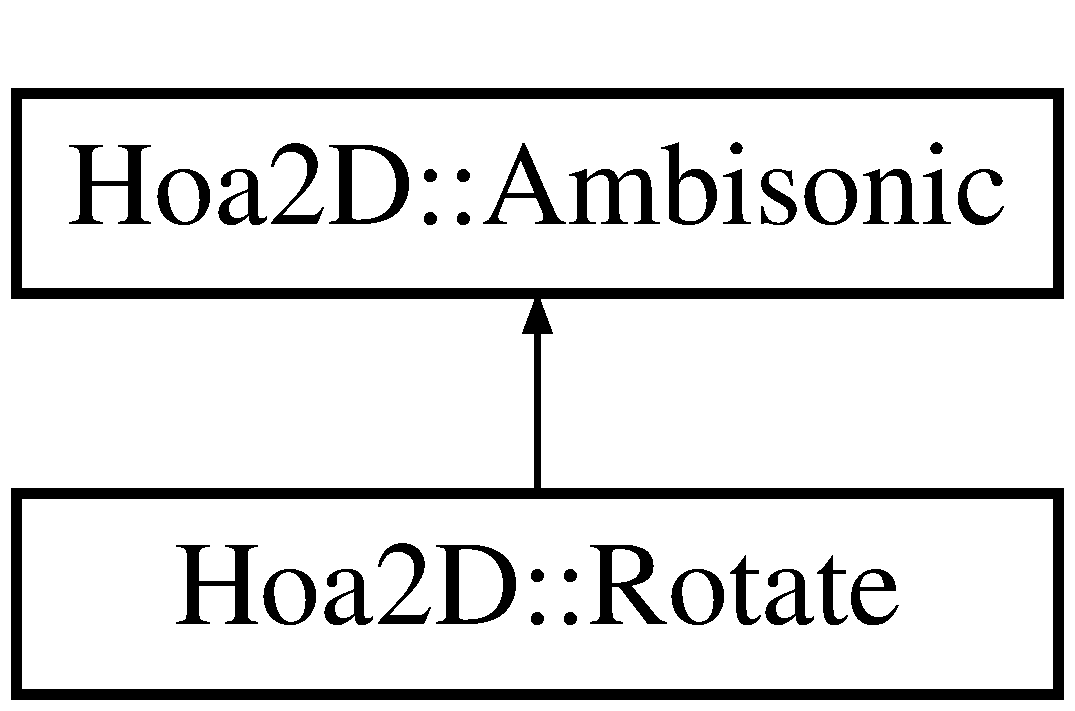
\includegraphics[height=2.000000cm]{class_hoa2_d_1_1_rotate}
\end{center}
\end{figure}
\subsection*{Public Member Functions}
\begin{DoxyCompactItemize}
\item 
\hyperlink{class_hoa2_d_1_1_rotate_a2aa145bb455c0538ce2ca2bd058d8800}{Rotate} (unsigned int order)
\begin{DoxyCompactList}\small\item\em The rotate constructor. \end{DoxyCompactList}\item 
\hyperlink{class_hoa2_d_1_1_rotate_a7e70e8d9099c1b8a2a42313e464130b2}{$\sim$\-Rotate} ()
\begin{DoxyCompactList}\small\item\em The \hyperlink{class_hoa2_d_1_1_rotate}{Rotate} destructor. \end{DoxyCompactList}\item 
void \hyperlink{class_hoa2_d_1_1_rotate_abc51eceaf32e9844d829a816094f6ac5}{set\-Yaw} (const double value)
\begin{DoxyCompactList}\small\item\em This method sets the angle of the rotation around the z axis, the yaw value,. \end{DoxyCompactList}\item 
double \hyperlink{class_hoa2_d_1_1_rotate_a5f40eff256bd5b845d6b4cfc046cd84e}{get\-Yaw} () const 
\begin{DoxyCompactList}\small\item\em Get the angle of the rotation around the z axis, the yaw value. \end{DoxyCompactList}\item 
void \hyperlink{class_hoa2_d_1_1_rotate_a88bfa68435d940b0c4c1ae0c97baeffd}{process} (const float $\ast$inputs, float $\ast$outputs)
\begin{DoxyCompactList}\small\item\em This method performs the rotation with single precision. \end{DoxyCompactList}\item 
void \hyperlink{class_hoa2_d_1_1_rotate_a8d5ecedca52ad2216efe218b5dcbf834}{process} (const double $\ast$inputs, double $\ast$outputs)
\begin{DoxyCompactList}\small\item\em This method performs the rotation with double precision. \end{DoxyCompactList}\end{DoxyCompactItemize}


\subsection{Detailed Description}
The ambisonic rotation. 

The rotate should be used to rotate the ambisonic soundfield. 

Definition at line 17 of file Rotate.\-h.



\subsection{Constructor \& Destructor Documentation}
\hypertarget{class_hoa2_d_1_1_rotate_a2aa145bb455c0538ce2ca2bd058d8800}{\index{Hoa2\-D\-::\-Rotate@{Hoa2\-D\-::\-Rotate}!Rotate@{Rotate}}
\index{Rotate@{Rotate}!Hoa2D::Rotate@{Hoa2\-D\-::\-Rotate}}
\subsubsection[{Rotate}]{\setlength{\rightskip}{0pt plus 5cm}Hoa2\-D\-::\-Rotate\-::\-Rotate (
\begin{DoxyParamCaption}
\item[{unsigned int}]{order}
\end{DoxyParamCaption}
)}}\label{class_hoa2_d_1_1_rotate_a2aa145bb455c0538ce2ca2bd058d8800}


The rotate constructor. 

The rotate constructor allocates and initialize the member values to computes spherical harmonics rotation depending on a decomposition order. The order must be at least 1.


\begin{DoxyParams}{Parameters}
{\em order} & The order. \\
\hline
\end{DoxyParams}


Definition at line 11 of file Rotate.\-cpp.

\hypertarget{class_hoa2_d_1_1_rotate_a7e70e8d9099c1b8a2a42313e464130b2}{\index{Hoa2\-D\-::\-Rotate@{Hoa2\-D\-::\-Rotate}!$\sim$\-Rotate@{$\sim$\-Rotate}}
\index{$\sim$\-Rotate@{$\sim$\-Rotate}!Hoa2D::Rotate@{Hoa2\-D\-::\-Rotate}}
\subsubsection[{$\sim$\-Rotate}]{\setlength{\rightskip}{0pt plus 5cm}Hoa2\-D\-::\-Rotate\-::$\sim$\-Rotate (
\begin{DoxyParamCaption}
{}
\end{DoxyParamCaption}
)}}\label{class_hoa2_d_1_1_rotate_a7e70e8d9099c1b8a2a42313e464130b2}


The \hyperlink{class_hoa2_d_1_1_rotate}{Rotate} destructor. 

The \hyperlink{class_hoa2_d_1_1_rotate}{Rotate} destructor free the memory. 

Definition at line 59 of file Rotate.\-cpp.



\subsection{Member Function Documentation}
\hypertarget{class_hoa2_d_1_1_rotate_a5f40eff256bd5b845d6b4cfc046cd84e}{\index{Hoa2\-D\-::\-Rotate@{Hoa2\-D\-::\-Rotate}!get\-Yaw@{get\-Yaw}}
\index{get\-Yaw@{get\-Yaw}!Hoa2D::Rotate@{Hoa2\-D\-::\-Rotate}}
\subsubsection[{get\-Yaw}]{\setlength{\rightskip}{0pt plus 5cm}double Hoa2\-D\-::\-Rotate\-::get\-Yaw (
\begin{DoxyParamCaption}
{}
\end{DoxyParamCaption}
) const\hspace{0.3cm}{\ttfamily [inline]}}}\label{class_hoa2_d_1_1_rotate_a5f40eff256bd5b845d6b4cfc046cd84e}


Get the angle of the rotation around the z axis, the yaw value. 

The method returns the angle of the rotation around the z axis, the yaw value, in radian between 0 and 2π.

\begin{DoxyReturn}{Returns}
The yaw value. 
\end{DoxyReturn}


Definition at line 51 of file Rotate.\-h.

\hypertarget{class_hoa2_d_1_1_rotate_a88bfa68435d940b0c4c1ae0c97baeffd}{\index{Hoa2\-D\-::\-Rotate@{Hoa2\-D\-::\-Rotate}!process@{process}}
\index{process@{process}!Hoa2D::Rotate@{Hoa2\-D\-::\-Rotate}}
\subsubsection[{process}]{\setlength{\rightskip}{0pt plus 5cm}void Hoa2\-D\-::\-Rotate\-::process (
\begin{DoxyParamCaption}
\item[{const float $\ast$}]{inputs, }
\item[{float $\ast$}]{outputs}
\end{DoxyParamCaption}
)}}\label{class_hoa2_d_1_1_rotate_a88bfa68435d940b0c4c1ae0c97baeffd}


This method performs the rotation with single precision. 

You should use this method for in-\/place or not-\/in-\/place processing and performs the rotation sample by sample. The inputs array and outputs array contains the spherical harmonics samples and the minimum size must be the number of harmonics.


\begin{DoxyParams}{Parameters}
{\em inputs} & The input array. \\
\hline
{\em outputs} & The output array. \\
\hline
\end{DoxyParams}


Definition at line 23 of file Rotate.\-cpp.

\hypertarget{class_hoa2_d_1_1_rotate_a8d5ecedca52ad2216efe218b5dcbf834}{\index{Hoa2\-D\-::\-Rotate@{Hoa2\-D\-::\-Rotate}!process@{process}}
\index{process@{process}!Hoa2D::Rotate@{Hoa2\-D\-::\-Rotate}}
\subsubsection[{process}]{\setlength{\rightskip}{0pt plus 5cm}void Hoa2\-D\-::\-Rotate\-::process (
\begin{DoxyParamCaption}
\item[{const double $\ast$}]{inputs, }
\item[{double $\ast$}]{outputs}
\end{DoxyParamCaption}
)}}\label{class_hoa2_d_1_1_rotate_a8d5ecedca52ad2216efe218b5dcbf834}


This method performs the rotation with double precision. 

You should use this method for in-\/place or not-\/in-\/place processing and performs the rotation sample by sample. The inputs array and outputs array contains the spherical harmonics samples and the minimum size must be the number of harmonics.


\begin{DoxyParams}{Parameters}
{\em inputs} & The input array. \\
\hline
{\em outputs} & The output array. \\
\hline
\end{DoxyParams}


Definition at line 41 of file Rotate.\-cpp.

\hypertarget{class_hoa2_d_1_1_rotate_abc51eceaf32e9844d829a816094f6ac5}{\index{Hoa2\-D\-::\-Rotate@{Hoa2\-D\-::\-Rotate}!set\-Yaw@{set\-Yaw}}
\index{set\-Yaw@{set\-Yaw}!Hoa2D::Rotate@{Hoa2\-D\-::\-Rotate}}
\subsubsection[{set\-Yaw}]{\setlength{\rightskip}{0pt plus 5cm}void Hoa2\-D\-::\-Rotate\-::set\-Yaw (
\begin{DoxyParamCaption}
\item[{const double}]{value}
\end{DoxyParamCaption}
)}}\label{class_hoa2_d_1_1_rotate_abc51eceaf32e9844d829a816094f6ac5}


This method sets the angle of the rotation around the z axis, the yaw value,. 

The yaw is equivalent to a rotation around the z axis, the value is in radian and should be between 0 and 2π.


\begin{DoxyParams}{Parameters}
{\em value} & The yaw value. \\
\hline
\end{DoxyParams}


Definition at line 16 of file Rotate.\-cpp.



The documentation for this class was generated from the following files\-:\begin{DoxyCompactItemize}
\item 
/\-Users/elioton/\-Documents/programmation/\-C\-I\-C\-M/source\-Tree/\-Hoa\-Library/\-Sources/\-Hoa2\-D/Rotate.\-h\item 
/\-Users/elioton/\-Documents/programmation/\-C\-I\-C\-M/source\-Tree/\-Hoa\-Library/\-Sources/\-Hoa2\-D/Rotate.\-cpp\end{DoxyCompactItemize}

\hypertarget{class_hoa3_d_1_1_rotate}{\section{Hoa3\-D\-:\-:Rotate Class Reference}
\label{class_hoa3_d_1_1_rotate}\index{Hoa3\-D\-::\-Rotate@{Hoa3\-D\-::\-Rotate}}
}


The ambisonic \hyperlink{class_hoa3_d_1_1_rotate}{Rotate}.  




{\ttfamily \#include $<$Rotate.\-h$>$}

Inheritance diagram for Hoa3\-D\-:\-:Rotate\-:\begin{figure}[H]
\begin{center}
\leavevmode
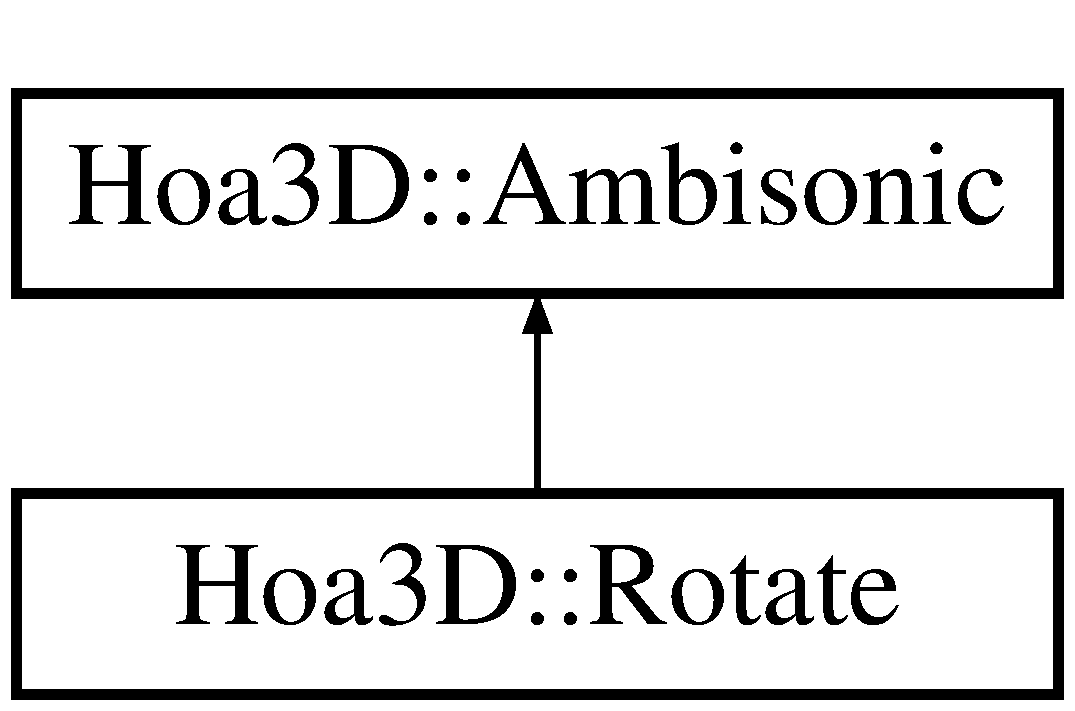
\includegraphics[height=2.000000cm]{class_hoa3_d_1_1_rotate}
\end{center}
\end{figure}
\subsection*{Public Member Functions}
\begin{DoxyCompactItemize}
\item 
\hyperlink{class_hoa3_d_1_1_rotate_a9a5750cbff8e0449b3de62e7de338a8b}{Rotate} (unsigned int order)
\begin{DoxyCompactList}\small\item\em The \hyperlink{class_hoa3_d_1_1_rotate}{Rotate} constructor. \end{DoxyCompactList}\item 
\hyperlink{class_hoa3_d_1_1_rotate_a13a37adfe31314b7d5844333a4e587ab}{$\sim$\-Rotate} ()
\begin{DoxyCompactList}\small\item\em The \hyperlink{class_hoa3_d_1_1_rotate}{Rotate} destructor. \end{DoxyCompactList}\item 
void \hyperlink{class_hoa3_d_1_1_rotate_a190ffb26419c5ab6c7935d48e9a7e23b}{set\-Rotations} (const double roll, const double pitch, const double yaw)
\begin{DoxyCompactList}\small\item\em This method sets the three rotation values at the same time (xyz axis). \end{DoxyCompactList}\item 
void \hyperlink{class_hoa3_d_1_1_rotate_a89599a9cd8c10240ce71b8fd7bdbb3b7}{set\-Roll} (const double value)
\begin{DoxyCompactList}\small\item\em This method sets the roll value (rotation on the x-\/axis). \end{DoxyCompactList}\item 
void \hyperlink{class_hoa3_d_1_1_rotate_aeb7e844c29c2f9bb9cc7de3ef89385f6}{set\-Pitch} (const double value)
\begin{DoxyCompactList}\small\item\em This method sets the pitch value (rotation on the y-\/axis). \end{DoxyCompactList}\item 
void \hyperlink{class_hoa3_d_1_1_rotate_a18df4eaec4e8c7c60f8234632af06d6f}{set\-Yaw} (const double value)
\begin{DoxyCompactList}\small\item\em This method sets the yaw value (rotation on the z-\/axis). \end{DoxyCompactList}\item 
double \hyperlink{class_hoa3_d_1_1_rotate_a4da29df01f2c7311490df11d4322b5f8}{get\-Roll} () const 
\begin{DoxyCompactList}\small\item\em Get the roll value (rotation on the x-\/axis). \end{DoxyCompactList}\item 
double \hyperlink{class_hoa3_d_1_1_rotate_afe1e5ccea5d375b082b7df2b8c8b972a}{get\-Pitch} () const 
\begin{DoxyCompactList}\small\item\em Get the pitch value (rotation on the y-\/axis). \end{DoxyCompactList}\item 
double \hyperlink{class_hoa3_d_1_1_rotate_a386f1fba4ceab4c2e243b7a222124d7e}{get\-Yaw} () const 
\begin{DoxyCompactList}\small\item\em Get the yaw value (rotation on the z-\/axis). \end{DoxyCompactList}\item 
void \hyperlink{class_hoa3_d_1_1_rotate_a9851055e9dbe808578e435c65f22c06a}{process} (const float $\ast$inputs, float $\ast$outputs)
\begin{DoxyCompactList}\small\item\em This method performs the rotation with single precision. \end{DoxyCompactList}\item 
void \hyperlink{class_hoa3_d_1_1_rotate_a395dafa6cc2d92562e6ac8044a438b2c}{process} (const double $\ast$inputs, double $\ast$outputs)
\begin{DoxyCompactList}\small\item\em This method performs the rotation with double precision. \end{DoxyCompactList}\end{DoxyCompactItemize}


\subsection{Detailed Description}
The ambisonic \hyperlink{class_hoa3_d_1_1_rotate}{Rotate}. 

The \hyperlink{class_hoa3_d_1_1_rotate}{Rotate} should be used to rotate an entire soundfield. 

Definition at line 18 of file Rotate.\-h.



\subsection{Constructor \& Destructor Documentation}
\hypertarget{class_hoa3_d_1_1_rotate_a9a5750cbff8e0449b3de62e7de338a8b}{\index{Hoa3\-D\-::\-Rotate@{Hoa3\-D\-::\-Rotate}!Rotate@{Rotate}}
\index{Rotate@{Rotate}!Hoa3D::Rotate@{Hoa3\-D\-::\-Rotate}}
\subsubsection[{Rotate}]{\setlength{\rightskip}{0pt plus 5cm}Hoa3\-D\-::\-Rotate\-::\-Rotate (
\begin{DoxyParamCaption}
\item[{unsigned int}]{order}
\end{DoxyParamCaption}
)}}\label{class_hoa3_d_1_1_rotate_a9a5750cbff8e0449b3de62e7de338a8b}


The \hyperlink{class_hoa3_d_1_1_rotate}{Rotate} constructor. 

The \hyperlink{class_hoa3_d_1_1_rotate}{Rotate} constructor allocates and initialize the member values to computes spherical harmonics rotation depending on a decomposition order. The order must be at least 1.


\begin{DoxyParams}{Parameters}
{\em order} & The order. \\
\hline
\end{DoxyParams}


Definition at line 11 of file Rotate.\-cpp.

\hypertarget{class_hoa3_d_1_1_rotate_a13a37adfe31314b7d5844333a4e587ab}{\index{Hoa3\-D\-::\-Rotate@{Hoa3\-D\-::\-Rotate}!$\sim$\-Rotate@{$\sim$\-Rotate}}
\index{$\sim$\-Rotate@{$\sim$\-Rotate}!Hoa3D::Rotate@{Hoa3\-D\-::\-Rotate}}
\subsubsection[{$\sim$\-Rotate}]{\setlength{\rightskip}{0pt plus 5cm}Hoa3\-D\-::\-Rotate\-::$\sim$\-Rotate (
\begin{DoxyParamCaption}
{}
\end{DoxyParamCaption}
)}}\label{class_hoa3_d_1_1_rotate_a13a37adfe31314b7d5844333a4e587ab}


The \hyperlink{class_hoa3_d_1_1_rotate}{Rotate} destructor. 

The \hyperlink{class_hoa3_d_1_1_rotate}{Rotate} destructor free the memory. 

Definition at line 85 of file Rotate.\-cpp.



\subsection{Member Function Documentation}
\hypertarget{class_hoa3_d_1_1_rotate_afe1e5ccea5d375b082b7df2b8c8b972a}{\index{Hoa3\-D\-::\-Rotate@{Hoa3\-D\-::\-Rotate}!get\-Pitch@{get\-Pitch}}
\index{get\-Pitch@{get\-Pitch}!Hoa3D::Rotate@{Hoa3\-D\-::\-Rotate}}
\subsubsection[{get\-Pitch}]{\setlength{\rightskip}{0pt plus 5cm}double Hoa3\-D\-::\-Rotate\-::get\-Pitch (
\begin{DoxyParamCaption}
{}
\end{DoxyParamCaption}
) const\hspace{0.3cm}{\ttfamily [inline]}}}\label{class_hoa3_d_1_1_rotate_afe1e5ccea5d375b082b7df2b8c8b972a}


Get the pitch value (rotation on the y-\/axis). 

The pitch is equivalent to a rotation on the y-\/axis (also named tumble).

\begin{DoxyReturn}{Returns}
value The pitch value between 0 and 2π. 
\end{DoxyReturn}


Definition at line 94 of file Rotate.\-h.

\hypertarget{class_hoa3_d_1_1_rotate_a4da29df01f2c7311490df11d4322b5f8}{\index{Hoa3\-D\-::\-Rotate@{Hoa3\-D\-::\-Rotate}!get\-Roll@{get\-Roll}}
\index{get\-Roll@{get\-Roll}!Hoa3D::Rotate@{Hoa3\-D\-::\-Rotate}}
\subsubsection[{get\-Roll}]{\setlength{\rightskip}{0pt plus 5cm}double Hoa3\-D\-::\-Rotate\-::get\-Roll (
\begin{DoxyParamCaption}
{}
\end{DoxyParamCaption}
) const\hspace{0.3cm}{\ttfamily [inline]}}}\label{class_hoa3_d_1_1_rotate_a4da29df01f2c7311490df11d4322b5f8}


Get the roll value (rotation on the x-\/axis). 

The roll is equivalent to a rotation on the x-\/axis (also named tilt).

\begin{DoxyReturn}{Returns}
value The roll value between 0 and 2π. 
\end{DoxyReturn}


Definition at line 87 of file Rotate.\-h.

\hypertarget{class_hoa3_d_1_1_rotate_a386f1fba4ceab4c2e243b7a222124d7e}{\index{Hoa3\-D\-::\-Rotate@{Hoa3\-D\-::\-Rotate}!get\-Yaw@{get\-Yaw}}
\index{get\-Yaw@{get\-Yaw}!Hoa3D::Rotate@{Hoa3\-D\-::\-Rotate}}
\subsubsection[{get\-Yaw}]{\setlength{\rightskip}{0pt plus 5cm}double Hoa3\-D\-::\-Rotate\-::get\-Yaw (
\begin{DoxyParamCaption}
{}
\end{DoxyParamCaption}
) const\hspace{0.3cm}{\ttfamily [inline]}}}\label{class_hoa3_d_1_1_rotate_a386f1fba4ceab4c2e243b7a222124d7e}


Get the yaw value (rotation on the z-\/axis). 

The yaw is equivalent to a rotation on the z-\/axis (also named rotation).

\begin{DoxyReturn}{Returns}
value The yaw value between 0 and 2π. 
\end{DoxyReturn}


Definition at line 101 of file Rotate.\-h.

\hypertarget{class_hoa3_d_1_1_rotate_a9851055e9dbe808578e435c65f22c06a}{\index{Hoa3\-D\-::\-Rotate@{Hoa3\-D\-::\-Rotate}!process@{process}}
\index{process@{process}!Hoa3D::Rotate@{Hoa3\-D\-::\-Rotate}}
\subsubsection[{process}]{\setlength{\rightskip}{0pt plus 5cm}void Hoa3\-D\-::\-Rotate\-::process (
\begin{DoxyParamCaption}
\item[{const float $\ast$}]{inputs, }
\item[{float $\ast$}]{outputs}
\end{DoxyParamCaption}
)}}\label{class_hoa3_d_1_1_rotate_a9851055e9dbe808578e435c65f22c06a}


This method performs the rotation with single precision. 

You should use this method for not-\/in-\/place processing and performs the rotation sample by sample. (warning \-: doesn't work with in-\/place vectors); The inputs array and outputs array contains the spherical harmonics samples and the minimum size must be the number of harmonics.


\begin{DoxyParams}{Parameters}
{\em inputs} & The input array. \\
\hline
{\em outputs} & The output array. \\
\hline
\end{DoxyParams}


Definition at line 47 of file Rotate.\-cpp.

\hypertarget{class_hoa3_d_1_1_rotate_a395dafa6cc2d92562e6ac8044a438b2c}{\index{Hoa3\-D\-::\-Rotate@{Hoa3\-D\-::\-Rotate}!process@{process}}
\index{process@{process}!Hoa3D::Rotate@{Hoa3\-D\-::\-Rotate}}
\subsubsection[{process}]{\setlength{\rightskip}{0pt plus 5cm}void Hoa3\-D\-::\-Rotate\-::process (
\begin{DoxyParamCaption}
\item[{const double $\ast$}]{inputs, }
\item[{double $\ast$}]{outputs}
\end{DoxyParamCaption}
)}}\label{class_hoa3_d_1_1_rotate_a395dafa6cc2d92562e6ac8044a438b2c}


This method performs the rotation with double precision. 

You should use this method for not-\/in-\/place processing and performs the rotation sample by sample. (warning \-: doesn't work with in-\/place vectors); The inputs array and outputs array contains the spherical harmonics samples and the minimum size must be the number of harmonics.


\begin{DoxyParams}{Parameters}
{\em inputs} & The input array. \\
\hline
{\em outputs} & The output array. \\
\hline
\end{DoxyParams}


Definition at line 53 of file Rotate.\-cpp.

\hypertarget{class_hoa3_d_1_1_rotate_aeb7e844c29c2f9bb9cc7de3ef89385f6}{\index{Hoa3\-D\-::\-Rotate@{Hoa3\-D\-::\-Rotate}!set\-Pitch@{set\-Pitch}}
\index{set\-Pitch@{set\-Pitch}!Hoa3D::Rotate@{Hoa3\-D\-::\-Rotate}}
\subsubsection[{set\-Pitch}]{\setlength{\rightskip}{0pt plus 5cm}void Hoa3\-D\-::\-Rotate\-::set\-Pitch (
\begin{DoxyParamCaption}
\item[{const double}]{value}
\end{DoxyParamCaption}
)}}\label{class_hoa3_d_1_1_rotate_aeb7e844c29c2f9bb9cc7de3ef89385f6}


This method sets the pitch value (rotation on the y-\/axis). 

The pitch is equivalent to a rotation on the y-\/axis (also named tumble).


\begin{DoxyParams}{Parameters}
{\em value} & The pitch value between 0 and 2π. \\
\hline
\end{DoxyParams}


Definition at line 34 of file Rotate.\-cpp.

\hypertarget{class_hoa3_d_1_1_rotate_a89599a9cd8c10240ce71b8fd7bdbb3b7}{\index{Hoa3\-D\-::\-Rotate@{Hoa3\-D\-::\-Rotate}!set\-Roll@{set\-Roll}}
\index{set\-Roll@{set\-Roll}!Hoa3D::Rotate@{Hoa3\-D\-::\-Rotate}}
\subsubsection[{set\-Roll}]{\setlength{\rightskip}{0pt plus 5cm}void Hoa3\-D\-::\-Rotate\-::set\-Roll (
\begin{DoxyParamCaption}
\item[{const double}]{value}
\end{DoxyParamCaption}
)}}\label{class_hoa3_d_1_1_rotate_a89599a9cd8c10240ce71b8fd7bdbb3b7}


This method sets the roll value (rotation on the x-\/axis). 

The roll is equivalent to a rotation on the x-\/axis (also named tilt).


\begin{DoxyParams}{Parameters}
{\em value} & The roll value between 0 and 2π. \\
\hline
\end{DoxyParams}


Definition at line 27 of file Rotate.\-cpp.

\hypertarget{class_hoa3_d_1_1_rotate_a190ffb26419c5ab6c7935d48e9a7e23b}{\index{Hoa3\-D\-::\-Rotate@{Hoa3\-D\-::\-Rotate}!set\-Rotations@{set\-Rotations}}
\index{set\-Rotations@{set\-Rotations}!Hoa3D::Rotate@{Hoa3\-D\-::\-Rotate}}
\subsubsection[{set\-Rotations}]{\setlength{\rightskip}{0pt plus 5cm}void Hoa3\-D\-::\-Rotate\-::set\-Rotations (
\begin{DoxyParamCaption}
\item[{const double}]{roll, }
\item[{const double}]{pitch, }
\item[{const double}]{yaw}
\end{DoxyParamCaption}
)}}\label{class_hoa3_d_1_1_rotate_a190ffb26419c5ab6c7935d48e9a7e23b}


This method sets the three rotation values at the same time (xyz axis). 

This method sets the three rotation values at the same time (xyz axis).


\begin{DoxyParams}{Parameters}
{\em roll} & The roll value is equivalent to a rotation on the x-\/axis (also named tilt), between 0 and 2π. \\
\hline
{\em pitch} & The pitch value is equivalent to a rotation on the y-\/axis (also named tumble), between 0 and 2π. \\
\hline
{\em yaw} & The yaw value is equivalent to a rotation on the z-\/axis (also named rotation), between 0 and 2π. \\
\hline
\end{DoxyParams}
\begin{DoxySeeAlso}{See Also}
\hyperlink{class_hoa3_d_1_1_rotate_a89599a9cd8c10240ce71b8fd7bdbb3b7}{set\-Roll}, \hyperlink{class_hoa3_d_1_1_rotate_aeb7e844c29c2f9bb9cc7de3ef89385f6}{set\-Pitch}, \hyperlink{class_hoa3_d_1_1_rotate_a18df4eaec4e8c7c60f8234632af06d6f}{set\-Yaw} 
\end{DoxySeeAlso}


Definition at line 20 of file Rotate.\-cpp.

\hypertarget{class_hoa3_d_1_1_rotate_a18df4eaec4e8c7c60f8234632af06d6f}{\index{Hoa3\-D\-::\-Rotate@{Hoa3\-D\-::\-Rotate}!set\-Yaw@{set\-Yaw}}
\index{set\-Yaw@{set\-Yaw}!Hoa3D::Rotate@{Hoa3\-D\-::\-Rotate}}
\subsubsection[{set\-Yaw}]{\setlength{\rightskip}{0pt plus 5cm}void Hoa3\-D\-::\-Rotate\-::set\-Yaw (
\begin{DoxyParamCaption}
\item[{const double}]{value}
\end{DoxyParamCaption}
)}}\label{class_hoa3_d_1_1_rotate_a18df4eaec4e8c7c60f8234632af06d6f}


This method sets the yaw value (rotation on the z-\/axis). 

The yaw is equivalent to a rotation on the z-\/axis (also named rotation).


\begin{DoxyParams}{Parameters}
{\em value} & The yaw value between 0 and 2π. \\
\hline
\end{DoxyParams}


Definition at line 39 of file Rotate.\-cpp.



The documentation for this class was generated from the following files\-:\begin{DoxyCompactItemize}
\item 
/\-Users/elioton/\-Documents/programmation/\-C\-I\-C\-M/source\-Tree/\-Hoa\-Library/\-Sources/\-Hoa3\-D/Rotate.\-h\item 
/\-Users/elioton/\-Documents/programmation/\-C\-I\-C\-M/source\-Tree/\-Hoa\-Library/\-Sources/\-Hoa3\-D/Rotate.\-cpp\end{DoxyCompactItemize}

\hypertarget{class_hoa3_d_1_1_scope}{\section{Hoa3\-D\-:\-:Scope Class Reference}
\label{class_hoa3_d_1_1_scope}\index{Hoa3\-D\-::\-Scope@{Hoa3\-D\-::\-Scope}}
}


The ambisonic scope.  




{\ttfamily \#include $<$Scope.\-h$>$}

Inheritance diagram for Hoa3\-D\-:\-:Scope\-:\begin{figure}[H]
\begin{center}
\leavevmode
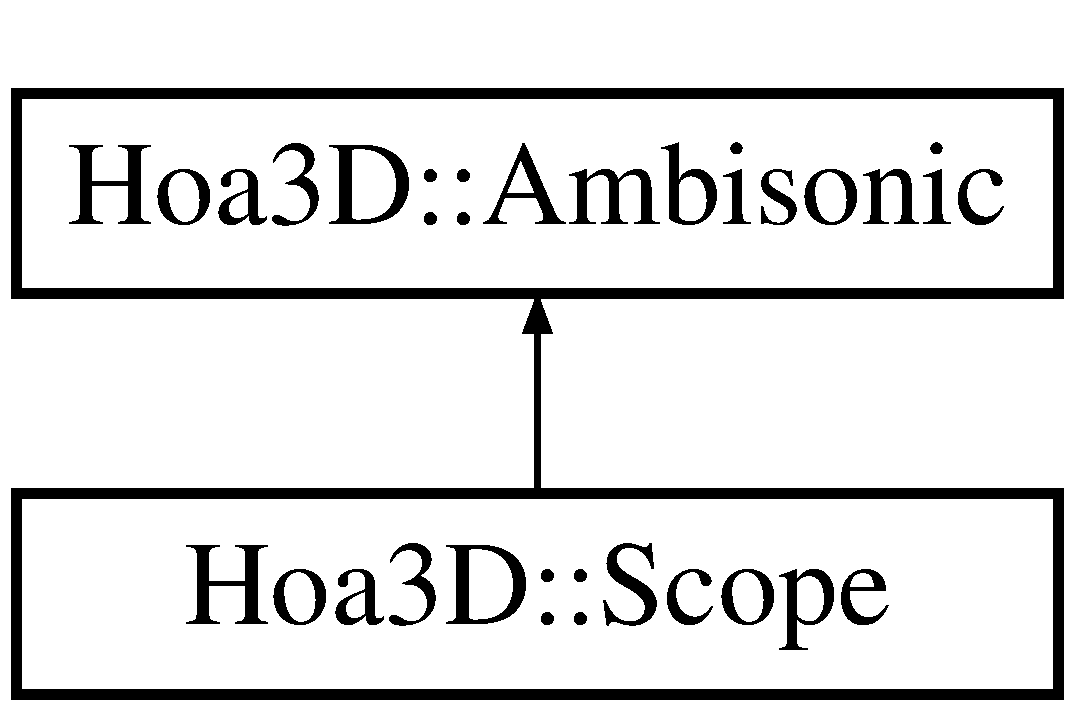
\includegraphics[height=2.000000cm]{class_hoa3_d_1_1_scope}
\end{center}
\end{figure}
\subsection*{Public Member Functions}
\begin{DoxyCompactItemize}
\item 
\hyperlink{class_hoa3_d_1_1_scope_ab4f5ff6674c4df165a1455e4648e1c35}{Scope} (unsigned int order, unsigned int number\-Of\-Rows, unsigned int number\-Of\-Columns)
\begin{DoxyCompactList}\small\item\em The \hyperlink{class_hoa3_d_1_1_scope}{Scope} constructor. \end{DoxyCompactList}\item 
\hyperlink{class_hoa3_d_1_1_scope_a84990cf90c7b3be0963f4cacbdab1df8}{$\sim$\-Scope} ()
\begin{DoxyCompactList}\small\item\em The \hyperlink{class_hoa3_d_1_1_scope}{Scope} destructor. \end{DoxyCompactList}\item 
unsigned int \hyperlink{class_hoa3_d_1_1_scope_aab635359344e855d855972752e6766c9}{get\-Number\-Of\-Rows} () const 
\begin{DoxyCompactList}\small\item\em Retrieve the number of rows. \end{DoxyCompactList}\item 
unsigned int \hyperlink{class_hoa3_d_1_1_scope_abdee40de6953ec537bbc72154ac93e6e}{get\-Number\-Of\-Columns} () const 
\begin{DoxyCompactList}\small\item\em Retrieve the number of column. \end{DoxyCompactList}\item 
double \hyperlink{class_hoa3_d_1_1_scope_a5dd62de174f903097d992da4f108037e}{get\-Value} (unsigned int row\-Index, unsigned int column\-Index) const 
\begin{DoxyCompactList}\small\item\em Retrieve the value of a point of the spherical harmonics projection. \end{DoxyCompactList}\item 
double \hyperlink{class_hoa3_d_1_1_scope_a2452963dd7f2ee7d61af6186d049db24}{get\-Radius} (unsigned int row\-Index, unsigned int column\-Index) const 
\begin{DoxyCompactList}\small\item\em Retrieve the radius of a point of the spherical harmonics projection. \end{DoxyCompactList}\item 
double \hyperlink{class_hoa3_d_1_1_scope_a9a0c8cf80dc5686b746fc3d5b742de45}{get\-Azimuth} (unsigned int column\-Index) const 
\begin{DoxyCompactList}\small\item\em Retrieve the azimuth of a point of the spherical harmonics projection. \end{DoxyCompactList}\item 
double \hyperlink{class_hoa3_d_1_1_scope_ab878f89077b6d2829bf00436aadd309b}{get\-Elevation} (unsigned int row\-Index) const 
\begin{DoxyCompactList}\small\item\em Retrieve the elevation of a point of the spherical harmonics projection. \end{DoxyCompactList}\item 
void \hyperlink{class_hoa3_d_1_1_scope_a4e9866933d1b863860ffd64b0514a6e6}{process} (const float $\ast$inputs)
\begin{DoxyCompactList}\small\item\em This method performs the spherical harmonics projection with single precision. \end{DoxyCompactList}\item 
void \hyperlink{class_hoa3_d_1_1_scope_ae9a788e0352011e3ad7ad5f88b5b12ed}{process} (const double $\ast$inputs)
\begin{DoxyCompactList}\small\item\em This method performs the spherical harmonics projection with double precision. \end{DoxyCompactList}\end{DoxyCompactItemize}


\subsection{Detailed Description}
The ambisonic scope. 

The scope discretize a sphere by a set of point and uses a decoder to project the spherical harmonics on it. This class should be used for graphical interfaces outside the digital signal processing if the number of points to discretize the sphere is very large. Then you should prefer to record snapshot of the spherical harmonics and to call the process method at an interval adapted to a graphical rendering. 

Definition at line 18 of file Scope.\-h.



\subsection{Constructor \& Destructor Documentation}
\hypertarget{class_hoa3_d_1_1_scope_ab4f5ff6674c4df165a1455e4648e1c35}{\index{Hoa3\-D\-::\-Scope@{Hoa3\-D\-::\-Scope}!Scope@{Scope}}
\index{Scope@{Scope}!Hoa3D::Scope@{Hoa3\-D\-::\-Scope}}
\subsubsection[{Scope}]{\setlength{\rightskip}{0pt plus 5cm}Hoa3\-D\-::\-Scope\-::\-Scope (
\begin{DoxyParamCaption}
\item[{unsigned int}]{order, }
\item[{unsigned int}]{number\-Of\-Rows, }
\item[{unsigned int}]{number\-Of\-Columns}
\end{DoxyParamCaption}
)}}\label{class_hoa3_d_1_1_scope_ab4f5ff6674c4df165a1455e4648e1c35}


The \hyperlink{class_hoa3_d_1_1_scope}{Scope} constructor. 

\begin{DoxyVerb}The Scope constructor allocates and initialize the member values to computes spherical harmonics projection on a sphere depending on a decomposition order and a sphere discretization. The sphere discretization is done by a set of points defined by rows and columns then the precision will be lower at the elevation center (0 radian) than at the top (1/2 Pi) or the bottom (-1/2 Pi) of the sphere. The number of row discretize the elevation then it set how many points are used between the bottom and the top. The number of column discretize the azimuth circle then it set how many points are used to make the turn from the front (O radian). Then the sphere is discretized by number of rows * number of columns points. The order must be at least 1. The number of rows and column should be at least 3 (but it's very low).
\end{DoxyVerb}



\begin{DoxyParams}{Parameters}
{\em order} & The order. \\
\hline
{\em number\-Of\-Row} & The number of rows. \\
\hline
{\em number\-Of\-Column} & The number of columns. \\
\hline
\end{DoxyParams}


Definition at line 11 of file Scope.\-cpp.

\hypertarget{class_hoa3_d_1_1_scope_a84990cf90c7b3be0963f4cacbdab1df8}{\index{Hoa3\-D\-::\-Scope@{Hoa3\-D\-::\-Scope}!$\sim$\-Scope@{$\sim$\-Scope}}
\index{$\sim$\-Scope@{$\sim$\-Scope}!Hoa3D::Scope@{Hoa3\-D\-::\-Scope}}
\subsubsection[{$\sim$\-Scope}]{\setlength{\rightskip}{0pt plus 5cm}Hoa3\-D\-::\-Scope\-::$\sim$\-Scope (
\begin{DoxyParamCaption}
{}
\end{DoxyParamCaption}
)}}\label{class_hoa3_d_1_1_scope_a84990cf90c7b3be0963f4cacbdab1df8}


The \hyperlink{class_hoa3_d_1_1_scope}{Scope} destructor. 

The \hyperlink{class_hoa3_d_1_1_scope}{Scope} destructor free the memory. 

Definition at line 54 of file Scope.\-cpp.



\subsection{Member Function Documentation}
\hypertarget{class_hoa3_d_1_1_scope_a9a0c8cf80dc5686b746fc3d5b742de45}{\index{Hoa3\-D\-::\-Scope@{Hoa3\-D\-::\-Scope}!get\-Azimuth@{get\-Azimuth}}
\index{get\-Azimuth@{get\-Azimuth}!Hoa3D::Scope@{Hoa3\-D\-::\-Scope}}
\subsubsection[{get\-Azimuth}]{\setlength{\rightskip}{0pt plus 5cm}double Hoa3\-D\-::\-Scope\-::get\-Azimuth (
\begin{DoxyParamCaption}
\item[{unsigned int}]{column\-Index}
\end{DoxyParamCaption}
) const\hspace{0.3cm}{\ttfamily [inline]}}}\label{class_hoa3_d_1_1_scope_a9a0c8cf80dc5686b746fc3d5b742de45}


Retrieve the azimuth of a point of the spherical harmonics projection. 

\begin{DoxyVerb}Retrieve the azimuth of the spherical harmonics projection for a given point defined by a row index and a column index. For the column index, 0 is the front (0 radian) and number of columns / 2 is the rear of the sphere. The maximum column index must be the number of columns - 1.
\end{DoxyVerb}



\begin{DoxyParams}{Parameters}
{\em row\-Index} & The row index of the point. \\
\hline
{\em column\-Index} & The column index of the point. \\
\hline
\end{DoxyParams}
\begin{DoxyReturn}{Returns}
This method returns the azimuth of a point of the ambisonic sphere. 
\end{DoxyReturn}
\begin{DoxySeeAlso}{See Also}
\hyperlink{class_hoa3_d_1_1_scope_a5dd62de174f903097d992da4f108037e}{get\-Value} 

\hyperlink{class_hoa3_d_1_1_scope_a2452963dd7f2ee7d61af6186d049db24}{get\-Radius} 

\hyperlink{class_hoa3_d_1_1_scope_ab878f89077b6d2829bf00436aadd309b}{get\-Elevation} 
\end{DoxySeeAlso}


Definition at line 106 of file Scope.\-h.

\hypertarget{class_hoa3_d_1_1_scope_ab878f89077b6d2829bf00436aadd309b}{\index{Hoa3\-D\-::\-Scope@{Hoa3\-D\-::\-Scope}!get\-Elevation@{get\-Elevation}}
\index{get\-Elevation@{get\-Elevation}!Hoa3D::Scope@{Hoa3\-D\-::\-Scope}}
\subsubsection[{get\-Elevation}]{\setlength{\rightskip}{0pt plus 5cm}double Hoa3\-D\-::\-Scope\-::get\-Elevation (
\begin{DoxyParamCaption}
\item[{unsigned int}]{row\-Index}
\end{DoxyParamCaption}
) const\hspace{0.3cm}{\ttfamily [inline]}}}\label{class_hoa3_d_1_1_scope_ab878f89077b6d2829bf00436aadd309b}


Retrieve the elevation of a point of the spherical harmonics projection. 

\begin{DoxyVerb}Retrieve the elevation of the spherical harmonics projection for a given point defined by a row index. For the row index, 0 is the bottom of the sphere, number of rows / 2 is at the center of the elevation and number of rows - 1 is at the top of the sphere. The maximum row index must be the number of row - 1.
\end{DoxyVerb}



\begin{DoxyParams}{Parameters}
{\em row\-Index} & The row index of the point. \\
\hline
{\em column\-Index} & The column index of the point. \\
\hline
\end{DoxyParams}
\begin{DoxyReturn}{Returns}
This method returns the elevation of a point of the ambisonic sphere. 
\end{DoxyReturn}
\begin{DoxySeeAlso}{See Also}
\hyperlink{class_hoa3_d_1_1_scope_a5dd62de174f903097d992da4f108037e}{get\-Value} 

\hyperlink{class_hoa3_d_1_1_scope_a2452963dd7f2ee7d61af6186d049db24}{get\-Radius} 

\hyperlink{class_hoa3_d_1_1_scope_a9a0c8cf80dc5686b746fc3d5b742de45}{get\-Azimuth} 
\end{DoxySeeAlso}


Definition at line 122 of file Scope.\-h.

\hypertarget{class_hoa3_d_1_1_scope_abdee40de6953ec537bbc72154ac93e6e}{\index{Hoa3\-D\-::\-Scope@{Hoa3\-D\-::\-Scope}!get\-Number\-Of\-Columns@{get\-Number\-Of\-Columns}}
\index{get\-Number\-Of\-Columns@{get\-Number\-Of\-Columns}!Hoa3D::Scope@{Hoa3\-D\-::\-Scope}}
\subsubsection[{get\-Number\-Of\-Columns}]{\setlength{\rightskip}{0pt plus 5cm}unsigned int Hoa3\-D\-::\-Scope\-::get\-Number\-Of\-Columns (
\begin{DoxyParamCaption}
{}
\end{DoxyParamCaption}
) const\hspace{0.3cm}{\ttfamily [inline]}}}\label{class_hoa3_d_1_1_scope_abdee40de6953ec537bbc72154ac93e6e}


Retrieve the number of column. 

\begin{DoxyVerb}Retrieve the number of column used to discretize the ambisonic sphere.
\end{DoxyVerb}


\begin{DoxyReturn}{Returns}
This method returns the number of column used to discretize the sphere. 
\end{DoxyReturn}


Definition at line 57 of file Scope.\-h.

\hypertarget{class_hoa3_d_1_1_scope_aab635359344e855d855972752e6766c9}{\index{Hoa3\-D\-::\-Scope@{Hoa3\-D\-::\-Scope}!get\-Number\-Of\-Rows@{get\-Number\-Of\-Rows}}
\index{get\-Number\-Of\-Rows@{get\-Number\-Of\-Rows}!Hoa3D::Scope@{Hoa3\-D\-::\-Scope}}
\subsubsection[{get\-Number\-Of\-Rows}]{\setlength{\rightskip}{0pt plus 5cm}unsigned int Hoa3\-D\-::\-Scope\-::get\-Number\-Of\-Rows (
\begin{DoxyParamCaption}
{}
\end{DoxyParamCaption}
) const\hspace{0.3cm}{\ttfamily [inline]}}}\label{class_hoa3_d_1_1_scope_aab635359344e855d855972752e6766c9}


Retrieve the number of rows. 

\begin{DoxyVerb}Retrieve the number of rows used to discretize the ambisonic sphere.
\end{DoxyVerb}


\begin{DoxyReturn}{Returns}
This method returns the number of rows used to discretize the sphere. 
\end{DoxyReturn}


Definition at line 47 of file Scope.\-h.

\hypertarget{class_hoa3_d_1_1_scope_a2452963dd7f2ee7d61af6186d049db24}{\index{Hoa3\-D\-::\-Scope@{Hoa3\-D\-::\-Scope}!get\-Radius@{get\-Radius}}
\index{get\-Radius@{get\-Radius}!Hoa3D::Scope@{Hoa3\-D\-::\-Scope}}
\subsubsection[{get\-Radius}]{\setlength{\rightskip}{0pt plus 5cm}double Hoa3\-D\-::\-Scope\-::get\-Radius (
\begin{DoxyParamCaption}
\item[{unsigned int}]{row\-Index, }
\item[{unsigned int}]{column\-Index}
\end{DoxyParamCaption}
) const\hspace{0.3cm}{\ttfamily [inline]}}}\label{class_hoa3_d_1_1_scope_a2452963dd7f2ee7d61af6186d049db24}


Retrieve the radius of a point of the spherical harmonics projection. 

\begin{DoxyVerb}Retrieve the radius of the spherical harmonics projection for a given point defined by a row index and a column index. This the absolute of the result of the projection. For the row index, 0 is the bottom of the sphere, number of rows / 2 is at the center of the elevation and number of rows - 1 is at the top of the sphere. For the column index, 0 is the front (0 radian) and number of columns / 2 is the rear of the sphere. The maximum row index must be the number of row - 1 and the maximum column index must be the number of columns - 1.
\end{DoxyVerb}



\begin{DoxyParams}{Parameters}
{\em row\-Index} & The row index of the point. \\
\hline
{\em column\-Index} & The column index of the point. \\
\hline
\end{DoxyParams}
\begin{DoxyReturn}{Returns}
This method returns the radius of a point of the ambisonic sphere. 
\end{DoxyReturn}
\begin{DoxySeeAlso}{See Also}
\hyperlink{class_hoa3_d_1_1_scope_a9a0c8cf80dc5686b746fc3d5b742de45}{get\-Azimuth} 

\hyperlink{class_hoa3_d_1_1_scope_ab878f89077b6d2829bf00436aadd309b}{get\-Elevation} 

\hyperlink{class_hoa3_d_1_1_scope_a5dd62de174f903097d992da4f108037e}{get\-Value} 
\end{DoxySeeAlso}


Definition at line 89 of file Scope.\-h.

\hypertarget{class_hoa3_d_1_1_scope_a5dd62de174f903097d992da4f108037e}{\index{Hoa3\-D\-::\-Scope@{Hoa3\-D\-::\-Scope}!get\-Value@{get\-Value}}
\index{get\-Value@{get\-Value}!Hoa3D::Scope@{Hoa3\-D\-::\-Scope}}
\subsubsection[{get\-Value}]{\setlength{\rightskip}{0pt plus 5cm}double Hoa3\-D\-::\-Scope\-::get\-Value (
\begin{DoxyParamCaption}
\item[{unsigned int}]{row\-Index, }
\item[{unsigned int}]{column\-Index}
\end{DoxyParamCaption}
) const\hspace{0.3cm}{\ttfamily [inline]}}}\label{class_hoa3_d_1_1_scope_a5dd62de174f903097d992da4f108037e}


Retrieve the value of a point of the spherical harmonics projection. 

\begin{DoxyVerb}Retrieve the result value of the spherical harmonics projection for a given point defined by a row index and a column index. The absolute of the value can be used as the radius of the point for a 3 dimentionnal representation. For the row index, 0 is the bottom of the sphere, number of rows / 2 is at the center of the elevation and number of rows - 1 is at the top of the sphere. For the column index, 0 is the front (0 radian) and number of columns / 2 is the rear of the sphere. The maximum row index must be the number of row - 1 and the maximum column index must be the number of columns - 1.
\end{DoxyVerb}



\begin{DoxyParams}{Parameters}
{\em row\-Index} & The row index of the point. \\
\hline
{\em column\-Index} & The column index of the point. \\
\hline
\end{DoxyParams}
\begin{DoxyReturn}{Returns}
This method returns the value of a point of the ambisonic sphere. 
\end{DoxyReturn}
\begin{DoxySeeAlso}{See Also}
getradius 

\hyperlink{class_hoa3_d_1_1_scope_a9a0c8cf80dc5686b746fc3d5b742de45}{get\-Azimuth} 

\hyperlink{class_hoa3_d_1_1_scope_ab878f89077b6d2829bf00436aadd309b}{get\-Elevation} 
\end{DoxySeeAlso}


Definition at line 72 of file Scope.\-h.

\hypertarget{class_hoa3_d_1_1_scope_a4e9866933d1b863860ffd64b0514a6e6}{\index{Hoa3\-D\-::\-Scope@{Hoa3\-D\-::\-Scope}!process@{process}}
\index{process@{process}!Hoa3D::Scope@{Hoa3\-D\-::\-Scope}}
\subsubsection[{process}]{\setlength{\rightskip}{0pt plus 5cm}void Hoa3\-D\-::\-Scope\-::process (
\begin{DoxyParamCaption}
\item[{const float $\ast$}]{inputs}
\end{DoxyParamCaption}
)}}\label{class_hoa3_d_1_1_scope_a4e9866933d1b863860ffd64b0514a6e6}


This method performs the spherical harmonics projection with single precision. 

\begin{DoxyVerb}You should use this method to compute the projection of the spherical harmonics over an ambisonics sphere. The inputs array contains the spherical harmonics samples and the minimum size must be the number of harmonics.
\end{DoxyVerb}



\begin{DoxyParams}{Parameters}
{\em inputs} & The inputs array. \\
\hline
\end{DoxyParams}


Definition at line 28 of file Scope.\-cpp.

\hypertarget{class_hoa3_d_1_1_scope_ae9a788e0352011e3ad7ad5f88b5b12ed}{\index{Hoa3\-D\-::\-Scope@{Hoa3\-D\-::\-Scope}!process@{process}}
\index{process@{process}!Hoa3D::Scope@{Hoa3\-D\-::\-Scope}}
\subsubsection[{process}]{\setlength{\rightskip}{0pt plus 5cm}void Hoa3\-D\-::\-Scope\-::process (
\begin{DoxyParamCaption}
\item[{const double $\ast$}]{inputs}
\end{DoxyParamCaption}
)}}\label{class_hoa3_d_1_1_scope_ae9a788e0352011e3ad7ad5f88b5b12ed}


This method performs the spherical harmonics projection with double precision. 

\begin{DoxyVerb}You should use this method to compute the projection of the spherical harmonics over an ambisonics sphere. The inputs array contains the spherical harmonics samples and the minimum size must be the number of harmonics.
\end{DoxyVerb}



\begin{DoxyParams}{Parameters}
{\em inputs} & The inputs array. \\
\hline
\end{DoxyParams}


Definition at line 43 of file Scope.\-cpp.



The documentation for this class was generated from the following files\-:\begin{DoxyCompactItemize}
\item 
/\-Users/\-Pierre/\-Source\-Tree/\-Hoa\-Library/\-Sources/\-Hoa3\-D/Scope.\-h\item 
/\-Users/\-Pierre/\-Source\-Tree/\-Hoa\-Library/\-Sources/\-Hoa3\-D/Scope.\-cpp\end{DoxyCompactItemize}

\hypertarget{class_sources_manager}{\section{Sources\-Manager Class Reference}
\label{class_sources_manager}\index{Sources\-Manager@{Sources\-Manager}}
}


{\ttfamily \#include $<$Ambisonic\-Sources\-Manager.\-h$>$}

\subsection*{Public Member Functions}
\begin{DoxyCompactItemize}
\item 
\hyperlink{class_sources_manager_a333ef82bab70b995bf0f658c894bee1b}{Sources\-Manager} (double a\-Maximum\-Limit\-Value=-\/1., long dead\-Or\-Alive=1)
\end{DoxyCompactItemize}


\subsection{Detailed Description}
\hyperlink{interface_hoa_library}{Hoa\-Library} \-: A High Order Ambisonics Library Copyright (c) 2012-\/2013 Julien Colafrancesco, Pierre Guillot, Eliott Paris, C\-I\-C\-M, Universite Paris-\/8. All rights reserved.

Website \-: \href{http://www.mshparisnord.fr/hoalibrary/}{\tt http\-://www.\-mshparisnord.\-fr/hoalibrary/} Contacts \-: \href{mailto:cicm.mshparisnord@gmail.com}{\tt cicm.\-mshparisnord@gmail.\-com}

Redistribution and use in source and binary forms, with or without modification, are permitted provided that the following conditions are met\-:


\begin{DoxyItemize}
\item Redistributions may not be sold, nor may they be used in a commercial product or activity.
\item Redistributions of source code must retain the above copyright notice, this list of conditions and the following disclaimer.
\item Redistributions in binary form must reproduce the above copyright notice, this list of conditions and the following disclaimer in the documentation and/or other materials provided with the distribution.
\item Neither the name of the C\-I\-C\-M nor the names of its contributors may be used to endorse or promote products derived from this software without specific prior written permission.
\end{DoxyItemize}

T\-H\-I\-S S\-O\-F\-T\-W\-A\-R\-E I\-S P\-R\-O\-V\-I\-D\-E\-D B\-Y T\-H\-E C\-O\-P\-Y\-R\-I\-G\-H\-T H\-O\-L\-D\-E\-R\-S A\-N\-D C\-O\-N\-T\-R\-I\-B\-U\-T\-O\-R\-S \char`\"{}\-A\-S I\-S\char`\"{} A\-N\-D A\-N\-Y E\-X\-P\-R\-E\-S\-S O\-R I\-M\-P\-L\-I\-E\-D W\-A\-R\-R\-A\-N\-T\-I\-E\-S, I\-N\-C\-L\-U\-D\-I\-N\-G, B\-U\-T N\-O\-T L\-I\-M\-I\-T\-E\-D T\-O, T\-H\-E I\-M\-P\-L\-I\-E\-D W\-A\-R\-R\-A\-N\-T\-I\-E\-S O\-F M\-E\-R\-C\-H\-A\-N\-T\-A\-B\-I\-L\-I\-T\-Y A\-N\-D F\-I\-T\-N\-E\-S\-S F\-O\-R A P\-A\-R\-T\-I\-C\-U\-L\-A\-R P\-U\-R\-P\-O\-S\-E A\-R\-E D\-I\-S\-C\-L\-A\-I\-M\-E\-D. I\-N N\-O E\-V\-E\-N\-T S\-H\-A\-L\-L T\-H\-E C\-O\-P\-Y\-R\-I\-G\-H\-T H\-O\-L\-D\-E\-R O\-R C\-O\-N\-T\-R\-I\-B\-U\-T\-O\-R\-S B\-E L\-I\-A\-B\-L\-E F\-O\-R A\-N\-Y D\-I\-R\-E\-C\-T, I\-N\-D\-I\-R\-E\-C\-T, I\-N\-C\-I\-D\-E\-N\-T\-A\-L, S\-P\-E\-C\-I\-A\-L, E\-X\-E\-M\-P\-L\-A\-R\-Y, O\-R C\-O\-N\-S\-E\-Q\-U\-E\-N\-T\-I\-A\-L D\-A\-M\-A\-G\-E\-S (I\-N\-C\-L\-U\-D\-I\-N\-G, B\-U\-T N\-O\-T L\-I\-M\-I\-T\-E\-D T\-O, P\-R\-O\-C\-U\-R\-E\-M\-E\-N\-T O\-F S\-U\-B\-S\-T\-I\-T\-U\-T\-E G\-O\-O\-D\-S O\-R S\-E\-R\-V\-I\-C\-E\-S; L\-O\-S\-S O\-F U\-S\-E, D\-A\-T\-A, O\-R P\-R\-O\-F\-I\-T\-S; O\-R B\-U\-S\-I\-N\-E\-S\-S I\-N\-T\-E\-R\-R\-U\-P\-T\-I\-O\-N) H\-O\-W\-E\-V\-E\-R C\-A\-U\-S\-E\-D A\-N\-D O\-N A\-N\-Y T\-H\-E\-O\-R\-Y O\-F L\-I\-A\-B\-I\-L\-I\-T\-Y, W\-H\-E\-T\-H\-E\-R I\-N C\-O\-N\-T\-R\-A\-C\-T, S\-T\-R\-I\-C\-T L\-I\-A\-B\-I\-L\-I\-T\-Y, O\-R T\-O\-R\-T (I\-N\-C\-L\-U\-D\-I\-N\-G N\-E\-G\-L\-I\-G\-E\-N\-C\-E O\-R O\-T\-H\-E\-R\-W\-I\-S\-E) A\-R\-I\-S\-I\-N\-G I\-N A\-N\-Y W\-A\-Y O\-U\-T O\-F T\-H\-E U\-S\-E O\-F T\-H\-I\-S S\-O\-F\-T\-W\-A\-R\-E, E\-V\-E\-N I\-F A\-D\-V\-I\-S\-E\-D O\-F T\-H\-E P\-O\-S\-S\-I\-B\-I\-L\-I\-T\-Y O\-F S\-U\-C\-H D\-A\-M\-A\-G\-E. 

Definition at line 32 of file Ambisonic\-Sources\-Manager.\-h.



\subsection{Constructor \& Destructor Documentation}
\hypertarget{class_sources_manager_a333ef82bab70b995bf0f658c894bee1b}{\index{Sources\-Manager@{Sources\-Manager}!Sources\-Manager@{Sources\-Manager}}
\index{Sources\-Manager@{Sources\-Manager}!SourcesManager@{Sources\-Manager}}
\subsubsection[{Sources\-Manager}]{\setlength{\rightskip}{0pt plus 5cm}Sources\-Manager\-::\-Sources\-Manager (
\begin{DoxyParamCaption}
\item[{double}]{a\-Maximum\-Limit\-Value = {\ttfamily -\/1.}, }
\item[{long}]{dead\-Or\-Alive = {\ttfamily 1}}
\end{DoxyParamCaption}
)}}\label{class_sources_manager_a333ef82bab70b995bf0f658c894bee1b}
\hyperlink{interface_hoa_library}{Hoa\-Library} \-: A High Order Ambisonics Library Copyright (c) 2012-\/2013 Julien Colafrancesco, Pierre Guillot, Eliott Paris, C\-I\-C\-M, Universite Paris-\/8. All rights reserved.

Website \-: \href{http://www.mshparisnord.fr/hoalibrary/}{\tt http\-://www.\-mshparisnord.\-fr/hoalibrary/} Contacts \-: \href{mailto:cicm.mshparisnord@gmail.com}{\tt cicm.\-mshparisnord@gmail.\-com}

Redistribution and use in source and binary forms, with or without modification, are permitted provided that the following conditions are met\-:


\begin{DoxyItemize}
\item Redistributions may not be sold, nor may they be used in a commercial product or activity.
\item Redistributions of source code must retain the above copyright notice, this list of conditions and the following disclaimer.
\item Redistributions in binary form must reproduce the above copyright notice, this list of conditions and the following disclaimer in the documentation and/or other materials provided with the distribution.
\item Neither the name of the C\-I\-C\-M nor the names of its contributors may be used to endorse or promote products derived from this software without specific prior written permission.
\end{DoxyItemize}

T\-H\-I\-S S\-O\-F\-T\-W\-A\-R\-E I\-S P\-R\-O\-V\-I\-D\-E\-D B\-Y T\-H\-E C\-O\-P\-Y\-R\-I\-G\-H\-T H\-O\-L\-D\-E\-R\-S A\-N\-D C\-O\-N\-T\-R\-I\-B\-U\-T\-O\-R\-S \char`\"{}\-A\-S I\-S\char`\"{} A\-N\-D A\-N\-Y E\-X\-P\-R\-E\-S\-S O\-R I\-M\-P\-L\-I\-E\-D W\-A\-R\-R\-A\-N\-T\-I\-E\-S, I\-N\-C\-L\-U\-D\-I\-N\-G, B\-U\-T N\-O\-T L\-I\-M\-I\-T\-E\-D T\-O, T\-H\-E I\-M\-P\-L\-I\-E\-D W\-A\-R\-R\-A\-N\-T\-I\-E\-S O\-F M\-E\-R\-C\-H\-A\-N\-T\-A\-B\-I\-L\-I\-T\-Y A\-N\-D F\-I\-T\-N\-E\-S\-S F\-O\-R A P\-A\-R\-T\-I\-C\-U\-L\-A\-R P\-U\-R\-P\-O\-S\-E A\-R\-E D\-I\-S\-C\-L\-A\-I\-M\-E\-D. I\-N N\-O E\-V\-E\-N\-T S\-H\-A\-L\-L T\-H\-E C\-O\-P\-Y\-R\-I\-G\-H\-T H\-O\-L\-D\-E\-R O\-R C\-O\-N\-T\-R\-I\-B\-U\-T\-O\-R\-S B\-E L\-I\-A\-B\-L\-E F\-O\-R A\-N\-Y D\-I\-R\-E\-C\-T, I\-N\-D\-I\-R\-E\-C\-T, I\-N\-C\-I\-D\-E\-N\-T\-A\-L, S\-P\-E\-C\-I\-A\-L, E\-X\-E\-M\-P\-L\-A\-R\-Y, O\-R C\-O\-N\-S\-E\-Q\-U\-E\-N\-T\-I\-A\-L D\-A\-M\-A\-G\-E\-S (I\-N\-C\-L\-U\-D\-I\-N\-G, B\-U\-T N\-O\-T L\-I\-M\-I\-T\-E\-D T\-O, P\-R\-O\-C\-U\-R\-E\-M\-E\-N\-T O\-F S\-U\-B\-S\-T\-I\-T\-U\-T\-E G\-O\-O\-D\-S O\-R S\-E\-R\-V\-I\-C\-E\-S; L\-O\-S\-S O\-F U\-S\-E, D\-A\-T\-A, O\-R P\-R\-O\-F\-I\-T\-S; O\-R B\-U\-S\-I\-N\-E\-S\-S I\-N\-T\-E\-R\-R\-U\-P\-T\-I\-O\-N) H\-O\-W\-E\-V\-E\-R C\-A\-U\-S\-E\-D A\-N\-D O\-N A\-N\-Y T\-H\-E\-O\-R\-Y O\-F L\-I\-A\-B\-I\-L\-I\-T\-Y, W\-H\-E\-T\-H\-E\-R I\-N C\-O\-N\-T\-R\-A\-C\-T, S\-T\-R\-I\-C\-T L\-I\-A\-B\-I\-L\-I\-T\-Y, O\-R T\-O\-R\-T (I\-N\-C\-L\-U\-D\-I\-N\-G N\-E\-G\-L\-I\-G\-E\-N\-C\-E O\-R O\-T\-H\-E\-R\-W\-I\-S\-E) A\-R\-I\-S\-I\-N\-G I\-N A\-N\-Y W\-A\-Y O\-U\-T O\-F T\-H\-E U\-S\-E O\-F T\-H\-I\-S S\-O\-F\-T\-W\-A\-R\-E, E\-V\-E\-N I\-F A\-D\-V\-I\-S\-E\-D O\-F T\-H\-E P\-O\-S\-S\-I\-B\-I\-L\-I\-T\-Y O\-F S\-U\-C\-H D\-A\-M\-A\-G\-E. 

Definition at line 28 of file Ambisonic\-Sources\-Manager.\-cpp.



The documentation for this class was generated from the following files\-:\begin{DoxyCompactItemize}
\item 
/\-Users/\-Pierre/\-Source\-Tree/\-Hoa\-Library/\-Sources/hoa\-Map/Ambisonic\-Sources\-Manager.\-h\item 
/\-Users/\-Pierre/\-Source\-Tree/\-Hoa\-Library/\-Sources/hoa\-Map/Ambisonic\-Sources\-Manager.\-cpp\end{DoxyCompactItemize}

\hypertarget{class_sources_preset}{\section{Sources\-Preset Class Reference}
\label{class_sources_preset}\index{Sources\-Preset@{Sources\-Preset}}
}


{\ttfamily \#include $<$Ambisonic\-Sources\-Preset.\-h$>$}

Inheritance diagram for Sources\-Preset\-:\begin{figure}[H]
\begin{center}
\leavevmode
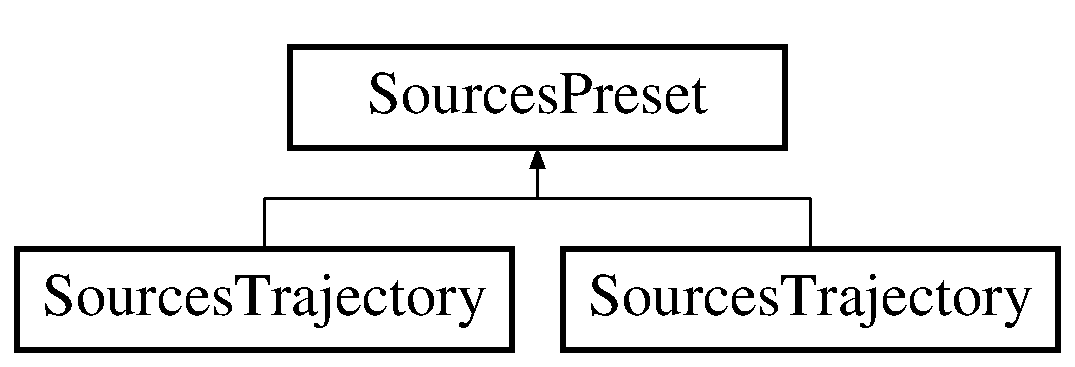
\includegraphics[height=2.000000cm]{class_sources_preset}
\end{center}
\end{figure}
\subsection*{Public Member Functions}
\begin{DoxyCompactItemize}
\item 
\hyperlink{class_sources_preset_a0a4203349327d10bb6afe35156126d8a}{Sources\-Preset} ()
\end{DoxyCompactItemize}


\subsection{Detailed Description}
Hoa\-Library \-: A High Order Ambisonics Library Copyright (c) 2012-\/2013 Julien Colafrancesco, Pierre Guillot, Eliott Paris, C\-I\-C\-M, Universite Paris-\/8. All rights reserved.

Website \-: \href{http://www.mshparisnord.fr/hoalibrary/}{\tt http\-://www.\-mshparisnord.\-fr/hoalibrary/} Contacts \-: \href{mailto:cicm.mshparisnord@gmail.com}{\tt cicm.\-mshparisnord@gmail.\-com}

Redistribution and use in source and binary forms, with or without modification, are permitted provided that the following conditions are met\-:


\begin{DoxyItemize}
\item Redistributions may not be sold, nor may they be used in a commercial product or activity.
\item Redistributions of source code must retain the above copyright notice, this list of conditions and the following disclaimer.
\item Redistributions in binary form must reproduce the above copyright notice, this list of conditions and the following disclaimer in the documentation and/or other materials provided with the distribution.
\item Neither the name of the C\-I\-C\-M nor the names of its contributors may be used to endorse or promote products derived from this software without specific prior written permission.
\end{DoxyItemize}

T\-H\-I\-S S\-O\-F\-T\-W\-A\-R\-E I\-S P\-R\-O\-V\-I\-D\-E\-D B\-Y T\-H\-E C\-O\-P\-Y\-R\-I\-G\-H\-T H\-O\-L\-D\-E\-R\-S A\-N\-D C\-O\-N\-T\-R\-I\-B\-U\-T\-O\-R\-S \char`\"{}\-A\-S I\-S\char`\"{} A\-N\-D A\-N\-Y E\-X\-P\-R\-E\-S\-S O\-R I\-M\-P\-L\-I\-E\-D W\-A\-R\-R\-A\-N\-T\-I\-E\-S, I\-N\-C\-L\-U\-D\-I\-N\-G, B\-U\-T N\-O\-T L\-I\-M\-I\-T\-E\-D T\-O, T\-H\-E I\-M\-P\-L\-I\-E\-D W\-A\-R\-R\-A\-N\-T\-I\-E\-S O\-F M\-E\-R\-C\-H\-A\-N\-T\-A\-B\-I\-L\-I\-T\-Y A\-N\-D F\-I\-T\-N\-E\-S\-S F\-O\-R A P\-A\-R\-T\-I\-C\-U\-L\-A\-R P\-U\-R\-P\-O\-S\-E A\-R\-E D\-I\-S\-C\-L\-A\-I\-M\-E\-D. I\-N N\-O E\-V\-E\-N\-T S\-H\-A\-L\-L T\-H\-E C\-O\-P\-Y\-R\-I\-G\-H\-T H\-O\-L\-D\-E\-R O\-R C\-O\-N\-T\-R\-I\-B\-U\-T\-O\-R\-S B\-E L\-I\-A\-B\-L\-E F\-O\-R A\-N\-Y D\-I\-R\-E\-C\-T, I\-N\-D\-I\-R\-E\-C\-T, I\-N\-C\-I\-D\-E\-N\-T\-A\-L, S\-P\-E\-C\-I\-A\-L, E\-X\-E\-M\-P\-L\-A\-R\-Y, O\-R C\-O\-N\-S\-E\-Q\-U\-E\-N\-T\-I\-A\-L D\-A\-M\-A\-G\-E\-S (I\-N\-C\-L\-U\-D\-I\-N\-G, B\-U\-T N\-O\-T L\-I\-M\-I\-T\-E\-D T\-O, P\-R\-O\-C\-U\-R\-E\-M\-E\-N\-T O\-F S\-U\-B\-S\-T\-I\-T\-U\-T\-E G\-O\-O\-D\-S O\-R S\-E\-R\-V\-I\-C\-E\-S; L\-O\-S\-S O\-F U\-S\-E, D\-A\-T\-A, O\-R P\-R\-O\-F\-I\-T\-S; O\-R B\-U\-S\-I\-N\-E\-S\-S I\-N\-T\-E\-R\-R\-U\-P\-T\-I\-O\-N) H\-O\-W\-E\-V\-E\-R C\-A\-U\-S\-E\-D A\-N\-D O\-N A\-N\-Y T\-H\-E\-O\-R\-Y O\-F L\-I\-A\-B\-I\-L\-I\-T\-Y, W\-H\-E\-T\-H\-E\-R I\-N C\-O\-N\-T\-R\-A\-C\-T, S\-T\-R\-I\-C\-T L\-I\-A\-B\-I\-L\-I\-T\-Y, O\-R T\-O\-R\-T (I\-N\-C\-L\-U\-D\-I\-N\-G N\-E\-G\-L\-I\-G\-E\-N\-C\-E O\-R O\-T\-H\-E\-R\-W\-I\-S\-E) A\-R\-I\-S\-I\-N\-G I\-N A\-N\-Y W\-A\-Y O\-U\-T O\-F T\-H\-E U\-S\-E O\-F T\-H\-I\-S S\-O\-F\-T\-W\-A\-R\-E, E\-V\-E\-N I\-F A\-D\-V\-I\-S\-E\-D O\-F T\-H\-E P\-O\-S\-S\-I\-B\-I\-L\-I\-T\-Y O\-F S\-U\-C\-H D\-A\-M\-A\-G\-E. 

Definition at line 31 of file Ambisonic\-Sources\-Preset.\-h.



\subsection{Constructor \& Destructor Documentation}
\hypertarget{class_sources_preset_a0a4203349327d10bb6afe35156126d8a}{\index{Sources\-Preset@{Sources\-Preset}!Sources\-Preset@{Sources\-Preset}}
\index{Sources\-Preset@{Sources\-Preset}!SourcesPreset@{Sources\-Preset}}
\subsubsection[{Sources\-Preset}]{\setlength{\rightskip}{0pt plus 5cm}Sources\-Preset\-::\-Sources\-Preset (
\begin{DoxyParamCaption}
{}
\end{DoxyParamCaption}
)}}\label{class_sources_preset_a0a4203349327d10bb6afe35156126d8a}
Hoa\-Library \-: A High Order Ambisonics Library Copyright (c) 2012-\/2013 Julien Colafrancesco, Pierre Guillot, Eliott Paris, C\-I\-C\-M, Universite Paris-\/8. All rights reserved.

Website \-: \href{http://www.mshparisnord.fr/hoalibrary/}{\tt http\-://www.\-mshparisnord.\-fr/hoalibrary/} Contacts \-: \href{mailto:cicm.mshparisnord@gmail.com}{\tt cicm.\-mshparisnord@gmail.\-com}

Redistribution and use in source and binary forms, with or without modification, are permitted provided that the following conditions are met\-:


\begin{DoxyItemize}
\item Redistributions may not be sold, nor may they be used in a commercial product or activity.
\item Redistributions of source code must retain the above copyright notice, this list of conditions and the following disclaimer.
\item Redistributions in binary form must reproduce the above copyright notice, this list of conditions and the following disclaimer in the documentation and/or other materials provided with the distribution.
\item Neither the name of the C\-I\-C\-M nor the names of its contributors may be used to endorse or promote products derived from this software without specific prior written permission.
\end{DoxyItemize}

T\-H\-I\-S S\-O\-F\-T\-W\-A\-R\-E I\-S P\-R\-O\-V\-I\-D\-E\-D B\-Y T\-H\-E C\-O\-P\-Y\-R\-I\-G\-H\-T H\-O\-L\-D\-E\-R\-S A\-N\-D C\-O\-N\-T\-R\-I\-B\-U\-T\-O\-R\-S \char`\"{}\-A\-S I\-S\char`\"{} A\-N\-D A\-N\-Y E\-X\-P\-R\-E\-S\-S O\-R I\-M\-P\-L\-I\-E\-D W\-A\-R\-R\-A\-N\-T\-I\-E\-S, I\-N\-C\-L\-U\-D\-I\-N\-G, B\-U\-T N\-O\-T L\-I\-M\-I\-T\-E\-D T\-O, T\-H\-E I\-M\-P\-L\-I\-E\-D W\-A\-R\-R\-A\-N\-T\-I\-E\-S O\-F M\-E\-R\-C\-H\-A\-N\-T\-A\-B\-I\-L\-I\-T\-Y A\-N\-D F\-I\-T\-N\-E\-S\-S F\-O\-R A P\-A\-R\-T\-I\-C\-U\-L\-A\-R P\-U\-R\-P\-O\-S\-E A\-R\-E D\-I\-S\-C\-L\-A\-I\-M\-E\-D. I\-N N\-O E\-V\-E\-N\-T S\-H\-A\-L\-L T\-H\-E C\-O\-P\-Y\-R\-I\-G\-H\-T H\-O\-L\-D\-E\-R O\-R C\-O\-N\-T\-R\-I\-B\-U\-T\-O\-R\-S B\-E L\-I\-A\-B\-L\-E F\-O\-R A\-N\-Y D\-I\-R\-E\-C\-T, I\-N\-D\-I\-R\-E\-C\-T, I\-N\-C\-I\-D\-E\-N\-T\-A\-L, S\-P\-E\-C\-I\-A\-L, E\-X\-E\-M\-P\-L\-A\-R\-Y, O\-R C\-O\-N\-S\-E\-Q\-U\-E\-N\-T\-I\-A\-L D\-A\-M\-A\-G\-E\-S (I\-N\-C\-L\-U\-D\-I\-N\-G, B\-U\-T N\-O\-T L\-I\-M\-I\-T\-E\-D T\-O, P\-R\-O\-C\-U\-R\-E\-M\-E\-N\-T O\-F S\-U\-B\-S\-T\-I\-T\-U\-T\-E G\-O\-O\-D\-S O\-R S\-E\-R\-V\-I\-C\-E\-S; L\-O\-S\-S O\-F U\-S\-E, D\-A\-T\-A, O\-R P\-R\-O\-F\-I\-T\-S; O\-R B\-U\-S\-I\-N\-E\-S\-S I\-N\-T\-E\-R\-R\-U\-P\-T\-I\-O\-N) H\-O\-W\-E\-V\-E\-R C\-A\-U\-S\-E\-D A\-N\-D O\-N A\-N\-Y T\-H\-E\-O\-R\-Y O\-F L\-I\-A\-B\-I\-L\-I\-T\-Y, W\-H\-E\-T\-H\-E\-R I\-N C\-O\-N\-T\-R\-A\-C\-T, S\-T\-R\-I\-C\-T L\-I\-A\-B\-I\-L\-I\-T\-Y, O\-R T\-O\-R\-T (I\-N\-C\-L\-U\-D\-I\-N\-G N\-E\-G\-L\-I\-G\-E\-N\-C\-E O\-R O\-T\-H\-E\-R\-W\-I\-S\-E) A\-R\-I\-S\-I\-N\-G I\-N A\-N\-Y W\-A\-Y O\-U\-T O\-F T\-H\-E U\-S\-E O\-F T\-H\-I\-S S\-O\-F\-T\-W\-A\-R\-E, E\-V\-E\-N I\-F A\-D\-V\-I\-S\-E\-D O\-F T\-H\-E P\-O\-S\-S\-I\-B\-I\-L\-I\-T\-Y O\-F S\-U\-C\-H D\-A\-M\-A\-G\-E. 

Definition at line 28 of file Ambisonic\-Sources\-Preset.\-cpp.



The documentation for this class was generated from the following files\-:\begin{DoxyCompactItemize}
\item 
/\-Users/elioton/\-Documents/programmation/\-C\-I\-C\-M/source\-Tree/\-Hoa\-Library/\-Sources/hoa\-Map/Ambisonic\-Sources\-Preset.\-h\item 
/\-Users/elioton/\-Documents/programmation/\-C\-I\-C\-M/source\-Tree/\-Hoa\-Library/\-Sources/hoa\-Map/Ambisonic\-Sources\-Preset.\-cpp\end{DoxyCompactItemize}

\hypertarget{class_sources_trajectory}{\section{Sources\-Trajectory Class Reference}
\label{class_sources_trajectory}\index{Sources\-Trajectory@{Sources\-Trajectory}}
}


{\ttfamily \#include $<$Ambisonic\-Sources\-Trajectory.\-h$>$}

Inheritance diagram for Sources\-Trajectory\-:\begin{figure}[H]
\begin{center}
\leavevmode
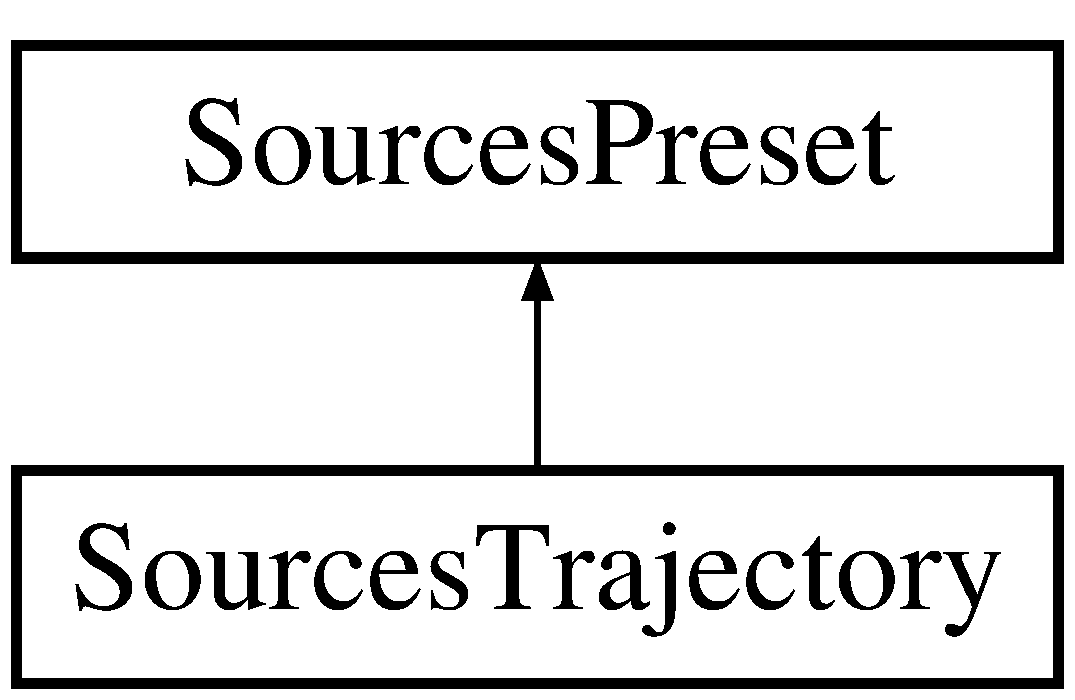
\includegraphics[height=2.000000cm]{class_sources_trajectory}
\end{center}
\end{figure}
\subsection*{Public Member Functions}
\begin{DoxyCompactItemize}
\item 
\hyperlink{class_sources_trajectory_a6e0838cc0ab29b5462cc624958498c4d}{Sources\-Trajectory} ()
\end{DoxyCompactItemize}


\subsection{Detailed Description}
Hoa\-Library \-: A High Order Ambisonics Library Copyright (c) 2012-\/2013 Julien Colafrancesco, Pierre Guillot, Eliott Paris, C\-I\-C\-M, Universite Paris-\/8. All rights reserved.

Website \-: \href{http://www.mshparisnord.fr/hoalibrary/}{\tt http\-://www.\-mshparisnord.\-fr/hoalibrary/} Contacts \-: \href{mailto:cicm.mshparisnord@gmail.com}{\tt cicm.\-mshparisnord@gmail.\-com}

Redistribution and use in source and binary forms, with or without modification, are permitted provided that the following conditions are met\-:


\begin{DoxyItemize}
\item Redistributions may not be sold, nor may they be used in a commercial product or activity.
\item Redistributions of source code must retain the above copyright notice, this list of conditions and the following disclaimer.
\item Redistributions in binary form must reproduce the above copyright notice, this list of conditions and the following disclaimer in the documentation and/or other materials provided with the distribution.
\item Neither the name of the C\-I\-C\-M nor the names of its contributors may be used to endorse or promote products derived from this software without specific prior written permission.
\end{DoxyItemize}

T\-H\-I\-S S\-O\-F\-T\-W\-A\-R\-E I\-S P\-R\-O\-V\-I\-D\-E\-D B\-Y T\-H\-E C\-O\-P\-Y\-R\-I\-G\-H\-T H\-O\-L\-D\-E\-R\-S A\-N\-D C\-O\-N\-T\-R\-I\-B\-U\-T\-O\-R\-S \char`\"{}\-A\-S I\-S\char`\"{} A\-N\-D A\-N\-Y E\-X\-P\-R\-E\-S\-S O\-R I\-M\-P\-L\-I\-E\-D W\-A\-R\-R\-A\-N\-T\-I\-E\-S, I\-N\-C\-L\-U\-D\-I\-N\-G, B\-U\-T N\-O\-T L\-I\-M\-I\-T\-E\-D T\-O, T\-H\-E I\-M\-P\-L\-I\-E\-D W\-A\-R\-R\-A\-N\-T\-I\-E\-S O\-F M\-E\-R\-C\-H\-A\-N\-T\-A\-B\-I\-L\-I\-T\-Y A\-N\-D F\-I\-T\-N\-E\-S\-S F\-O\-R A P\-A\-R\-T\-I\-C\-U\-L\-A\-R P\-U\-R\-P\-O\-S\-E A\-R\-E D\-I\-S\-C\-L\-A\-I\-M\-E\-D. I\-N N\-O E\-V\-E\-N\-T S\-H\-A\-L\-L T\-H\-E C\-O\-P\-Y\-R\-I\-G\-H\-T H\-O\-L\-D\-E\-R O\-R C\-O\-N\-T\-R\-I\-B\-U\-T\-O\-R\-S B\-E L\-I\-A\-B\-L\-E F\-O\-R A\-N\-Y D\-I\-R\-E\-C\-T, I\-N\-D\-I\-R\-E\-C\-T, I\-N\-C\-I\-D\-E\-N\-T\-A\-L, S\-P\-E\-C\-I\-A\-L, E\-X\-E\-M\-P\-L\-A\-R\-Y, O\-R C\-O\-N\-S\-E\-Q\-U\-E\-N\-T\-I\-A\-L D\-A\-M\-A\-G\-E\-S (I\-N\-C\-L\-U\-D\-I\-N\-G, B\-U\-T N\-O\-T L\-I\-M\-I\-T\-E\-D T\-O, P\-R\-O\-C\-U\-R\-E\-M\-E\-N\-T O\-F S\-U\-B\-S\-T\-I\-T\-U\-T\-E G\-O\-O\-D\-S O\-R S\-E\-R\-V\-I\-C\-E\-S; L\-O\-S\-S O\-F U\-S\-E, D\-A\-T\-A, O\-R P\-R\-O\-F\-I\-T\-S; O\-R B\-U\-S\-I\-N\-E\-S\-S I\-N\-T\-E\-R\-R\-U\-P\-T\-I\-O\-N) H\-O\-W\-E\-V\-E\-R C\-A\-U\-S\-E\-D A\-N\-D O\-N A\-N\-Y T\-H\-E\-O\-R\-Y O\-F L\-I\-A\-B\-I\-L\-I\-T\-Y, W\-H\-E\-T\-H\-E\-R I\-N C\-O\-N\-T\-R\-A\-C\-T, S\-T\-R\-I\-C\-T L\-I\-A\-B\-I\-L\-I\-T\-Y, O\-R T\-O\-R\-T (I\-N\-C\-L\-U\-D\-I\-N\-G N\-E\-G\-L\-I\-G\-E\-N\-C\-E O\-R O\-T\-H\-E\-R\-W\-I\-S\-E) A\-R\-I\-S\-I\-N\-G I\-N A\-N\-Y W\-A\-Y O\-U\-T O\-F T\-H\-E U\-S\-E O\-F T\-H\-I\-S S\-O\-F\-T\-W\-A\-R\-E, E\-V\-E\-N I\-F A\-D\-V\-I\-S\-E\-D O\-F T\-H\-E P\-O\-S\-S\-I\-B\-I\-L\-I\-T\-Y O\-F S\-U\-C\-H D\-A\-M\-A\-G\-E. 

Definition at line 31 of file Ambisonic\-Sources\-Trajectory.\-h.



\subsection{Constructor \& Destructor Documentation}
\hypertarget{class_sources_trajectory_a6e0838cc0ab29b5462cc624958498c4d}{\index{Sources\-Trajectory@{Sources\-Trajectory}!Sources\-Trajectory@{Sources\-Trajectory}}
\index{Sources\-Trajectory@{Sources\-Trajectory}!SourcesTrajectory@{Sources\-Trajectory}}
\subsubsection[{Sources\-Trajectory}]{\setlength{\rightskip}{0pt plus 5cm}Sources\-Trajectory\-::\-Sources\-Trajectory (
\begin{DoxyParamCaption}
{}
\end{DoxyParamCaption}
)}}\label{class_sources_trajectory_a6e0838cc0ab29b5462cc624958498c4d}
Hoa\-Library \-: A High Order Ambisonics Library Copyright (c) 2012-\/2013 Julien Colafrancesco, Pierre Guillot, Eliott Paris, C\-I\-C\-M, Universite Paris-\/8. All rights reserved.

Website \-: \href{http://www.mshparisnord.fr/hoalibrary/}{\tt http\-://www.\-mshparisnord.\-fr/hoalibrary/} Contacts \-: \href{mailto:cicm.mshparisnord@gmail.com}{\tt cicm.\-mshparisnord@gmail.\-com}

Redistribution and use in source and binary forms, with or without modification, are permitted provided that the following conditions are met\-:


\begin{DoxyItemize}
\item Redistributions may not be sold, nor may they be used in a commercial product or activity.
\item Redistributions of source code must retain the above copyright notice, this list of conditions and the following disclaimer.
\item Redistributions in binary form must reproduce the above copyright notice, this list of conditions and the following disclaimer in the documentation and/or other materials provided with the distribution.
\item Neither the name of the C\-I\-C\-M nor the names of its contributors may be used to endorse or promote products derived from this software without specific prior written permission.
\end{DoxyItemize}

T\-H\-I\-S S\-O\-F\-T\-W\-A\-R\-E I\-S P\-R\-O\-V\-I\-D\-E\-D B\-Y T\-H\-E C\-O\-P\-Y\-R\-I\-G\-H\-T H\-O\-L\-D\-E\-R\-S A\-N\-D C\-O\-N\-T\-R\-I\-B\-U\-T\-O\-R\-S \char`\"{}\-A\-S I\-S\char`\"{} A\-N\-D A\-N\-Y E\-X\-P\-R\-E\-S\-S O\-R I\-M\-P\-L\-I\-E\-D W\-A\-R\-R\-A\-N\-T\-I\-E\-S, I\-N\-C\-L\-U\-D\-I\-N\-G, B\-U\-T N\-O\-T L\-I\-M\-I\-T\-E\-D T\-O, T\-H\-E I\-M\-P\-L\-I\-E\-D W\-A\-R\-R\-A\-N\-T\-I\-E\-S O\-F M\-E\-R\-C\-H\-A\-N\-T\-A\-B\-I\-L\-I\-T\-Y A\-N\-D F\-I\-T\-N\-E\-S\-S F\-O\-R A P\-A\-R\-T\-I\-C\-U\-L\-A\-R P\-U\-R\-P\-O\-S\-E A\-R\-E D\-I\-S\-C\-L\-A\-I\-M\-E\-D. I\-N N\-O E\-V\-E\-N\-T S\-H\-A\-L\-L T\-H\-E C\-O\-P\-Y\-R\-I\-G\-H\-T H\-O\-L\-D\-E\-R O\-R C\-O\-N\-T\-R\-I\-B\-U\-T\-O\-R\-S B\-E L\-I\-A\-B\-L\-E F\-O\-R A\-N\-Y D\-I\-R\-E\-C\-T, I\-N\-D\-I\-R\-E\-C\-T, I\-N\-C\-I\-D\-E\-N\-T\-A\-L, S\-P\-E\-C\-I\-A\-L, E\-X\-E\-M\-P\-L\-A\-R\-Y, O\-R C\-O\-N\-S\-E\-Q\-U\-E\-N\-T\-I\-A\-L D\-A\-M\-A\-G\-E\-S (I\-N\-C\-L\-U\-D\-I\-N\-G, B\-U\-T N\-O\-T L\-I\-M\-I\-T\-E\-D T\-O, P\-R\-O\-C\-U\-R\-E\-M\-E\-N\-T O\-F S\-U\-B\-S\-T\-I\-T\-U\-T\-E G\-O\-O\-D\-S O\-R S\-E\-R\-V\-I\-C\-E\-S; L\-O\-S\-S O\-F U\-S\-E, D\-A\-T\-A, O\-R P\-R\-O\-F\-I\-T\-S; O\-R B\-U\-S\-I\-N\-E\-S\-S I\-N\-T\-E\-R\-R\-U\-P\-T\-I\-O\-N) H\-O\-W\-E\-V\-E\-R C\-A\-U\-S\-E\-D A\-N\-D O\-N A\-N\-Y T\-H\-E\-O\-R\-Y O\-F L\-I\-A\-B\-I\-L\-I\-T\-Y, W\-H\-E\-T\-H\-E\-R I\-N C\-O\-N\-T\-R\-A\-C\-T, S\-T\-R\-I\-C\-T L\-I\-A\-B\-I\-L\-I\-T\-Y, O\-R T\-O\-R\-T (I\-N\-C\-L\-U\-D\-I\-N\-G N\-E\-G\-L\-I\-G\-E\-N\-C\-E O\-R O\-T\-H\-E\-R\-W\-I\-S\-E) A\-R\-I\-S\-I\-N\-G I\-N A\-N\-Y W\-A\-Y O\-U\-T O\-F T\-H\-E U\-S\-E O\-F T\-H\-I\-S S\-O\-F\-T\-W\-A\-R\-E, E\-V\-E\-N I\-F A\-D\-V\-I\-S\-E\-D O\-F T\-H\-E P\-O\-S\-S\-I\-B\-I\-L\-I\-T\-Y O\-F S\-U\-C\-H D\-A\-M\-A\-G\-E. 

Definition at line 28 of file Ambisonic\-Sources\-Trajectory.\-cpp.



The documentation for this class was generated from the following files\-:\begin{DoxyCompactItemize}
\item 
/\-Users/elioton/\-Documents/programmation/\-C\-I\-C\-M/source\-Tree/\-Hoa\-Library/\-Sources/hoa\-Map/Ambisonic\-Sources\-Trajectory.\-h\item 
/\-Users/elioton/\-Documents/programmation/\-C\-I\-C\-M/source\-Tree/\-Hoa\-Library/\-Sources/hoa\-Map/Ambisonic\-Sources\-Trajectory.\-cpp\end{DoxyCompactItemize}

\hypertarget{class_tools}{\section{Tools Class Reference}
\label{class_tools}\index{Tools@{Tools}}
}


\subsection{Detailed Description}


Definition at line 68 of file Cicm\-Tools.\-h.



The documentation for this class was generated from the following file\-:\begin{DoxyCompactItemize}
\item 
/\-Users/\-Pierre/\-Source\-Tree/\-Hoa\-Library/\-Sources/\-Cicm\-Library/Cicm\-Tools.\-h\end{DoxyCompactItemize}

\hypertarget{class_hoa3_d_1_1_vector}{\section{Hoa3\-D\-:\-:Vector Class Reference}
\label{class_hoa3_d_1_1_vector}\index{Hoa3\-D\-::\-Vector@{Hoa3\-D\-::\-Vector}}
}


The ambisonic vector.  




{\ttfamily \#include $<$Vector.\-h$>$}

Inheritance diagram for Hoa3\-D\-:\-:Vector\-:\begin{figure}[H]
\begin{center}
\leavevmode
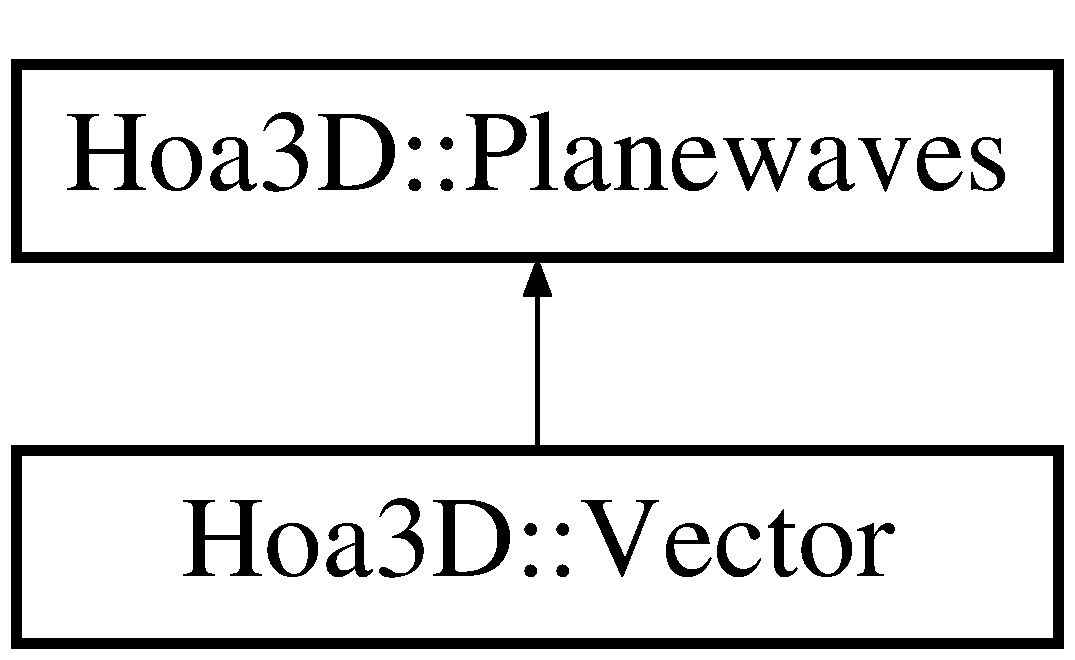
\includegraphics[height=2.000000cm]{class_hoa3_d_1_1_vector}
\end{center}
\end{figure}
\subsection*{Public Member Functions}
\begin{DoxyCompactItemize}
\item 
\hyperlink{class_hoa3_d_1_1_vector_a0a3ee9bd9477f9d20e123691c2e80315}{Vector} (unsigned int number\-Of\-Loudspeakers)
\begin{DoxyCompactList}\small\item\em The vector constructor. \end{DoxyCompactList}\item 
\hyperlink{class_hoa3_d_1_1_vector_a0f7403e0ae42fe40f54fcb35977bf95c}{$\sim$\-Vector} ()
\begin{DoxyCompactList}\small\item\em The optimization destructor. \end{DoxyCompactList}\item 
void \hyperlink{class_hoa3_d_1_1_vector_afab0f404886f74f5a139210d1a497936}{set\-Loudspeaker\-Position} (unsigned int index, double azimuth, double elevation)
\begin{DoxyCompactList}\small\item\em Set the position of a loudspeaker. \end{DoxyCompactList}\item 
void \hyperlink{class_hoa3_d_1_1_vector_a7818f4b944e66d27f08de1965c18e2bd}{process} (const float $\ast$inputs, float $\ast$outputs)
\begin{DoxyCompactList}\small\item\em This method compute the energy and velocity vectors with single precision. \end{DoxyCompactList}\item 
void \hyperlink{class_hoa3_d_1_1_vector_abf7d541dea71e683dda0aa494d843a64}{process} (const double $\ast$inputs, double $\ast$outputs)
\begin{DoxyCompactList}\small\item\em This method compute the energy and velocity vectors with double precision. \end{DoxyCompactList}\item 
void \hyperlink{class_hoa3_d_1_1_vector_a9c875cc6ac2171c5d8e1b8c1d466a844}{process\-Velocity} (const float $\ast$inputs, float $\ast$outputs)
\begin{DoxyCompactList}\small\item\em This method compute the velocity vector with single precision. \end{DoxyCompactList}\item 
void \hyperlink{class_hoa3_d_1_1_vector_a34ae72be81e72815e057e716a0f24d36}{process\-Velocity} (const double $\ast$inputs, double $\ast$outputs)
\begin{DoxyCompactList}\small\item\em This method compute the velocity vector with double precision. \end{DoxyCompactList}\item 
void \hyperlink{class_hoa3_d_1_1_vector_a7abd76a93ade46d069c922064f14c1b7}{process\-Energy} (const float $\ast$inputs, float $\ast$outputs)
\begin{DoxyCompactList}\small\item\em This method compute the energy vector with single precision. \end{DoxyCompactList}\item 
void \hyperlink{class_hoa3_d_1_1_vector_a28ad63d95b4d2c1ccabdada1955f5f96}{process\-Energy} (const double $\ast$inputs, double $\ast$outputs)
\begin{DoxyCompactList}\small\item\em This method compute the energy vector with double precision. \end{DoxyCompactList}\item 
\hyperlink{class_hoa3_d_1_1_vector_a0a3ee9bd9477f9d20e123691c2e80315}{Vector} (unsigned int number\-Of\-Loudspeakers)
\begin{DoxyCompactList}\small\item\em The vector constructor. \end{DoxyCompactList}\item 
\hyperlink{class_hoa3_d_1_1_vector_a0f7403e0ae42fe40f54fcb35977bf95c}{$\sim$\-Vector} ()
\begin{DoxyCompactList}\small\item\em The optimization destructor. \end{DoxyCompactList}\item 
void \hyperlink{class_hoa3_d_1_1_vector_afab0f404886f74f5a139210d1a497936}{set\-Loudspeaker\-Position} (unsigned int index, double azimuth, double elevation)
\begin{DoxyCompactList}\small\item\em Set the position of a loudspeaker. \end{DoxyCompactList}\item 
void \hyperlink{class_hoa3_d_1_1_vector_a7818f4b944e66d27f08de1965c18e2bd}{process} (const float $\ast$inputs, float $\ast$outputs)
\begin{DoxyCompactList}\small\item\em This method compute the energy and velocity vectors with single precision. \end{DoxyCompactList}\item 
void \hyperlink{class_hoa3_d_1_1_vector_abf7d541dea71e683dda0aa494d843a64}{process} (const double $\ast$inputs, double $\ast$outputs)
\begin{DoxyCompactList}\small\item\em This method compute the energy and velocity vectors with double precision. \end{DoxyCompactList}\item 
void \hyperlink{class_hoa3_d_1_1_vector_a9c875cc6ac2171c5d8e1b8c1d466a844}{process\-Velocity} (const float $\ast$inputs, float $\ast$outputs)
\begin{DoxyCompactList}\small\item\em This method compute the velocity vector with single precision. \end{DoxyCompactList}\item 
void \hyperlink{class_hoa3_d_1_1_vector_a34ae72be81e72815e057e716a0f24d36}{process\-Velocity} (const double $\ast$inputs, double $\ast$outputs)
\begin{DoxyCompactList}\small\item\em This method compute the velocity vector with double precision. \end{DoxyCompactList}\item 
void \hyperlink{class_hoa3_d_1_1_vector_a7abd76a93ade46d069c922064f14c1b7}{process\-Energy} (const float $\ast$inputs, float $\ast$outputs)
\begin{DoxyCompactList}\small\item\em This method compute the energy vector with single precision. \end{DoxyCompactList}\item 
void \hyperlink{class_hoa3_d_1_1_vector_a28ad63d95b4d2c1ccabdada1955f5f96}{process\-Energy} (const double $\ast$inputs, double $\ast$outputs)
\begin{DoxyCompactList}\small\item\em This method compute the energy vector with double precision. \end{DoxyCompactList}\end{DoxyCompactItemize}


\subsection{Detailed Description}
The ambisonic vector. 

The planewaves vector.

The vector class compute the energy and the velocity vector of a soudfield with signal of a spjerical set of loudspeakers. It is an useful tool to characterize the quality of the sound field resitution. For futher information \-: Michael A. Gerzon, General metatheorie of auditory localisation. Audio Engineering Society Preprint, 3306, 1992. This class retreive the cartesian coordinates of the vectors, the abscissa, the ordinate and the height. 

Definition at line 17 of file Vector.\-h.



\subsection{Constructor \& Destructor Documentation}
\hypertarget{class_hoa3_d_1_1_vector_a0a3ee9bd9477f9d20e123691c2e80315}{\index{Hoa3\-D\-::\-Vector@{Hoa3\-D\-::\-Vector}!Vector@{Vector}}
\index{Vector@{Vector}!Hoa3D::Vector@{Hoa3\-D\-::\-Vector}}
\subsubsection[{Vector}]{\setlength{\rightskip}{0pt plus 5cm}Hoa3\-D\-::\-Vector\-::\-Vector (
\begin{DoxyParamCaption}
\item[{unsigned int}]{number\-Of\-Loudspeakers}
\end{DoxyParamCaption}
)}}\label{class_hoa3_d_1_1_vector_a0a3ee9bd9477f9d20e123691c2e80315}


The vector constructor. 

The optimization constructor allocates and initialize the member values to computes vectors. The number\-Of\-Loudspeakers must be at least 1.


\begin{DoxyParams}{Parameters}
{\em number\-Of\-Loudspeakers} & The number of loudspeakers. \\
\hline
\end{DoxyParams}


Definition at line 11 of file Vector.\-cpp.

\hypertarget{class_hoa3_d_1_1_vector_a0f7403e0ae42fe40f54fcb35977bf95c}{\index{Hoa3\-D\-::\-Vector@{Hoa3\-D\-::\-Vector}!$\sim$\-Vector@{$\sim$\-Vector}}
\index{$\sim$\-Vector@{$\sim$\-Vector}!Hoa3D::Vector@{Hoa3\-D\-::\-Vector}}
\subsubsection[{$\sim$\-Vector}]{\setlength{\rightskip}{0pt plus 5cm}Hoa3\-D\-::\-Vector\-::$\sim$\-Vector (
\begin{DoxyParamCaption}
{}
\end{DoxyParamCaption}
)}}\label{class_hoa3_d_1_1_vector_a0f7403e0ae42fe40f54fcb35977bf95c}


The optimization destructor. 

The optimization destructor free the memory. 

Definition at line 151 of file Vector.\-cpp.

\hypertarget{class_hoa3_d_1_1_vector_a0a3ee9bd9477f9d20e123691c2e80315}{\index{Hoa3\-D\-::\-Vector@{Hoa3\-D\-::\-Vector}!Vector@{Vector}}
\index{Vector@{Vector}!Hoa3D::Vector@{Hoa3\-D\-::\-Vector}}
\subsubsection[{Vector}]{\setlength{\rightskip}{0pt plus 5cm}Hoa3\-D\-::\-Vector\-::\-Vector (
\begin{DoxyParamCaption}
\item[{unsigned int}]{number\-Of\-Loudspeakers}
\end{DoxyParamCaption}
)}}\label{class_hoa3_d_1_1_vector_a0a3ee9bd9477f9d20e123691c2e80315}


The vector constructor. 

The optimization constructor allocates and initialize the member values to computes vectors. The number\-Of\-Loudspeakers must be at least 1.


\begin{DoxyParams}{Parameters}
{\em number\-Of\-Loudspeakers} & The number of loudspeakers. \\
\hline
\end{DoxyParams}
\hypertarget{class_hoa3_d_1_1_vector_a0f7403e0ae42fe40f54fcb35977bf95c}{\index{Hoa3\-D\-::\-Vector@{Hoa3\-D\-::\-Vector}!$\sim$\-Vector@{$\sim$\-Vector}}
\index{$\sim$\-Vector@{$\sim$\-Vector}!Hoa3D::Vector@{Hoa3\-D\-::\-Vector}}
\subsubsection[{$\sim$\-Vector}]{\setlength{\rightskip}{0pt plus 5cm}Hoa3\-D\-::\-Vector\-::$\sim$\-Vector (
\begin{DoxyParamCaption}
{}
\end{DoxyParamCaption}
)}}\label{class_hoa3_d_1_1_vector_a0f7403e0ae42fe40f54fcb35977bf95c}


The optimization destructor. 

The optimization destructor free the memory. 

\subsection{Member Function Documentation}
\hypertarget{class_hoa3_d_1_1_vector_a7818f4b944e66d27f08de1965c18e2bd}{\index{Hoa3\-D\-::\-Vector@{Hoa3\-D\-::\-Vector}!process@{process}}
\index{process@{process}!Hoa3D::Vector@{Hoa3\-D\-::\-Vector}}
\subsubsection[{process}]{\setlength{\rightskip}{0pt plus 5cm}void Hoa3\-D\-::\-Vector\-::process (
\begin{DoxyParamCaption}
\item[{const float $\ast$}]{inputs, }
\item[{float $\ast$}]{outputs}
\end{DoxyParamCaption}
)}}\label{class_hoa3_d_1_1_vector_a7818f4b944e66d27f08de1965c18e2bd}


This method compute the energy and velocity vectors with single precision. 

You should use this method for in-\/place or not-\/in-\/place processing and compute the vectors sample by sample. The inputs array and contains the spherical harmonics samples and the minimum size must be the number of harmonics. The outputs array contains the vectors cartesian coordinates and the minimum size must be 6. The coordinates arrengement in the outputs array is velocity abscissa, velocity ordinate, velocity height, energy abscissa, energy ordinate, energy height.


\begin{DoxyParams}{Parameters}
{\em inputs} & The inputs array. \\
\hline
{\em outputs} & The outputs array. \\
\hline
\end{DoxyParams}


Definition at line 139 of file Vector.\-cpp.

\hypertarget{class_hoa3_d_1_1_vector_a7818f4b944e66d27f08de1965c18e2bd}{\index{Hoa3\-D\-::\-Vector@{Hoa3\-D\-::\-Vector}!process@{process}}
\index{process@{process}!Hoa3D::Vector@{Hoa3\-D\-::\-Vector}}
\subsubsection[{process}]{\setlength{\rightskip}{0pt plus 5cm}void Hoa3\-D\-::\-Vector\-::process (
\begin{DoxyParamCaption}
\item[{const float $\ast$}]{inputs, }
\item[{float $\ast$}]{outputs}
\end{DoxyParamCaption}
)}}\label{class_hoa3_d_1_1_vector_a7818f4b944e66d27f08de1965c18e2bd}


This method compute the energy and velocity vectors with single precision. 

You should use this method for in-\/place or not-\/in-\/place processing and compute the vectors sample by sample. The inputs array and contains the spherical harmonics samples and the minimum size must be the number of harmonics. The outputs array contains the vectors cartesian coordinates and the minimum size must be 6. The coordinates arrengement in the outputs array is velocity abscissa, velocity ordinate, velocity height, energy abscissa, energy ordinate, energy height.


\begin{DoxyParams}{Parameters}
{\em inputs} & The inputs array. \\
\hline
{\em outputs} & The outputs array. \\
\hline
\end{DoxyParams}
\hypertarget{class_hoa3_d_1_1_vector_abf7d541dea71e683dda0aa494d843a64}{\index{Hoa3\-D\-::\-Vector@{Hoa3\-D\-::\-Vector}!process@{process}}
\index{process@{process}!Hoa3D::Vector@{Hoa3\-D\-::\-Vector}}
\subsubsection[{process}]{\setlength{\rightskip}{0pt plus 5cm}void Hoa3\-D\-::\-Vector\-::process (
\begin{DoxyParamCaption}
\item[{const double $\ast$}]{inputs, }
\item[{double $\ast$}]{outputs}
\end{DoxyParamCaption}
)}}\label{class_hoa3_d_1_1_vector_abf7d541dea71e683dda0aa494d843a64}


This method compute the energy and velocity vectors with double precision. 

You should use this method for in-\/place or not-\/in-\/place processing and compute the vectors sample by sample. The inputs array and contains the spherical harmonics samples and the minimum size must be the number of harmonics. The outputs array contains the vectors cartesian coordinates and the minimum size must be 6. The coordinates arrengement in the outputs array is velocity abscissa, velocity ordinate, velocity height, energy abscissa, energy ordinate, energy height.


\begin{DoxyParams}{Parameters}
{\em inputs} & The inputs array. \\
\hline
{\em outputs} & The outputs array. \\
\hline
\end{DoxyParams}
\hypertarget{class_hoa3_d_1_1_vector_abf7d541dea71e683dda0aa494d843a64}{\index{Hoa3\-D\-::\-Vector@{Hoa3\-D\-::\-Vector}!process@{process}}
\index{process@{process}!Hoa3D::Vector@{Hoa3\-D\-::\-Vector}}
\subsubsection[{process}]{\setlength{\rightskip}{0pt plus 5cm}void Hoa3\-D\-::\-Vector\-::process (
\begin{DoxyParamCaption}
\item[{const double $\ast$}]{inputs, }
\item[{double $\ast$}]{outputs}
\end{DoxyParamCaption}
)}}\label{class_hoa3_d_1_1_vector_abf7d541dea71e683dda0aa494d843a64}


This method compute the energy and velocity vectors with double precision. 

You should use this method for in-\/place or not-\/in-\/place processing and compute the vectors sample by sample. The inputs array and contains the spherical harmonics samples and the minimum size must be the number of harmonics. The outputs array contains the vectors cartesian coordinates and the minimum size must be 6. The coordinates arrengement in the outputs array is velocity abscissa, velocity ordinate, velocity height, energy abscissa, energy ordinate, energy height.


\begin{DoxyParams}{Parameters}
{\em inputs} & The inputs array. \\
\hline
{\em outputs} & The outputs array. \\
\hline
\end{DoxyParams}


Definition at line 145 of file Vector.\-cpp.

\hypertarget{class_hoa3_d_1_1_vector_a7abd76a93ade46d069c922064f14c1b7}{\index{Hoa3\-D\-::\-Vector@{Hoa3\-D\-::\-Vector}!process\-Energy@{process\-Energy}}
\index{process\-Energy@{process\-Energy}!Hoa3D::Vector@{Hoa3\-D\-::\-Vector}}
\subsubsection[{process\-Energy}]{\setlength{\rightskip}{0pt plus 5cm}void Hoa3\-D\-::\-Vector\-::process\-Energy (
\begin{DoxyParamCaption}
\item[{const float $\ast$}]{inputs, }
\item[{float $\ast$}]{outputs}
\end{DoxyParamCaption}
)}}\label{class_hoa3_d_1_1_vector_a7abd76a93ade46d069c922064f14c1b7}


This method compute the energy vector with single precision. 

\begin{DoxyVerb}You should use this method for in-place or not-in-place processing and compute the vectors sample by sample. The inputs array and contains the spherical harmonics samples and the minimum size must be the number of harmonics. The outputs array contains the vectors cartesian coordinates and the minimum size must be 3. The coordinates arrengement in the outputs array is energy abscissa, energy ordinate, energy height.
\end{DoxyVerb}



\begin{DoxyParams}{Parameters}
{\em inputs} & The inputs array. \\
\hline
{\em outputs} & The outputs array. \\
\hline
\end{DoxyParams}
\hypertarget{class_hoa3_d_1_1_vector_a7abd76a93ade46d069c922064f14c1b7}{\index{Hoa3\-D\-::\-Vector@{Hoa3\-D\-::\-Vector}!process\-Energy@{process\-Energy}}
\index{process\-Energy@{process\-Energy}!Hoa3D::Vector@{Hoa3\-D\-::\-Vector}}
\subsubsection[{process\-Energy}]{\setlength{\rightskip}{0pt plus 5cm}void Hoa3\-D\-::\-Vector\-::process\-Energy (
\begin{DoxyParamCaption}
\item[{const float $\ast$}]{inputs, }
\item[{float $\ast$}]{outputs}
\end{DoxyParamCaption}
)}}\label{class_hoa3_d_1_1_vector_a7abd76a93ade46d069c922064f14c1b7}


This method compute the energy vector with single precision. 

\begin{DoxyVerb}You should use this method for in-place or not-in-place processing and compute the vectors sample by sample. The inputs array and contains the spherical harmonics samples and the minimum size must be the number of harmonics. The outputs array contains the vectors cartesian coordinates and the minimum size must be 3. The coordinates arrengement in the outputs array is energy abscissa, energy ordinate, energy height.
\end{DoxyVerb}



\begin{DoxyParams}{Parameters}
{\em inputs} & The inputs array. \\
\hline
{\em outputs} & The outputs array. \\
\hline
\end{DoxyParams}


Definition at line 86 of file Vector.\-cpp.

\hypertarget{class_hoa3_d_1_1_vector_a28ad63d95b4d2c1ccabdada1955f5f96}{\index{Hoa3\-D\-::\-Vector@{Hoa3\-D\-::\-Vector}!process\-Energy@{process\-Energy}}
\index{process\-Energy@{process\-Energy}!Hoa3D::Vector@{Hoa3\-D\-::\-Vector}}
\subsubsection[{process\-Energy}]{\setlength{\rightskip}{0pt plus 5cm}void Hoa3\-D\-::\-Vector\-::process\-Energy (
\begin{DoxyParamCaption}
\item[{const double $\ast$}]{inputs, }
\item[{double $\ast$}]{outputs}
\end{DoxyParamCaption}
)}}\label{class_hoa3_d_1_1_vector_a28ad63d95b4d2c1ccabdada1955f5f96}


This method compute the energy vector with double precision. 

\begin{DoxyVerb}You should use this method for in-place or not-in-place processing and compute the vectors sample by sample. The inputs array and contains the spherical harmonics samples and the minimum size must be the number of harmonics. The outputs array contains the vectors cartesian coordinates and the minimum size must be 3. The coordinates arrengement in the outputs array is energy abscissa, energy ordinate, energy height.
\end{DoxyVerb}



\begin{DoxyParams}{Parameters}
{\em inputs} & The inputs array. \\
\hline
{\em outputs} & The outputs array. \\
\hline
\end{DoxyParams}
\hypertarget{class_hoa3_d_1_1_vector_a28ad63d95b4d2c1ccabdada1955f5f96}{\index{Hoa3\-D\-::\-Vector@{Hoa3\-D\-::\-Vector}!process\-Energy@{process\-Energy}}
\index{process\-Energy@{process\-Energy}!Hoa3D::Vector@{Hoa3\-D\-::\-Vector}}
\subsubsection[{process\-Energy}]{\setlength{\rightskip}{0pt plus 5cm}void Hoa3\-D\-::\-Vector\-::process\-Energy (
\begin{DoxyParamCaption}
\item[{const double $\ast$}]{inputs, }
\item[{double $\ast$}]{outputs}
\end{DoxyParamCaption}
)}}\label{class_hoa3_d_1_1_vector_a28ad63d95b4d2c1ccabdada1955f5f96}


This method compute the energy vector with double precision. 

\begin{DoxyVerb}You should use this method for in-place or not-in-place processing and compute the vectors sample by sample. The inputs array and contains the spherical harmonics samples and the minimum size must be the number of harmonics. The outputs array contains the vectors cartesian coordinates and the minimum size must be 3. The coordinates arrengement in the outputs array is energy abscissa, energy ordinate, energy height.
\end{DoxyVerb}



\begin{DoxyParams}{Parameters}
{\em inputs} & The inputs array. \\
\hline
{\em outputs} & The outputs array. \\
\hline
\end{DoxyParams}


Definition at line 112 of file Vector.\-cpp.

\hypertarget{class_hoa3_d_1_1_vector_a9c875cc6ac2171c5d8e1b8c1d466a844}{\index{Hoa3\-D\-::\-Vector@{Hoa3\-D\-::\-Vector}!process\-Velocity@{process\-Velocity}}
\index{process\-Velocity@{process\-Velocity}!Hoa3D::Vector@{Hoa3\-D\-::\-Vector}}
\subsubsection[{process\-Velocity}]{\setlength{\rightskip}{0pt plus 5cm}void Hoa3\-D\-::\-Vector\-::process\-Velocity (
\begin{DoxyParamCaption}
\item[{const float $\ast$}]{inputs, }
\item[{float $\ast$}]{outputs}
\end{DoxyParamCaption}
)}}\label{class_hoa3_d_1_1_vector_a9c875cc6ac2171c5d8e1b8c1d466a844}


This method compute the velocity vector with single precision. 

\begin{DoxyVerb}You should use this method for in-place or not-in-place processing and compute the vectors sample by sample. The inputs array and contains the spherical harmonics samples and the minimum size must be the number of harmonics. The outputs array contains the vectors cartesian coordinates and the minimum size must be 3. The coordinates arrengement in the outputs array is velocity abscissa, velocity ordinate, velocity height.
\end{DoxyVerb}



\begin{DoxyParams}{Parameters}
{\em inputs} & The inputs array. \\
\hline
{\em outputs} & The outputs array. \\
\hline
\end{DoxyParams}


Definition at line 41 of file Vector.\-cpp.

\hypertarget{class_hoa3_d_1_1_vector_a9c875cc6ac2171c5d8e1b8c1d466a844}{\index{Hoa3\-D\-::\-Vector@{Hoa3\-D\-::\-Vector}!process\-Velocity@{process\-Velocity}}
\index{process\-Velocity@{process\-Velocity}!Hoa3D::Vector@{Hoa3\-D\-::\-Vector}}
\subsubsection[{process\-Velocity}]{\setlength{\rightskip}{0pt plus 5cm}void Hoa3\-D\-::\-Vector\-::process\-Velocity (
\begin{DoxyParamCaption}
\item[{const float $\ast$}]{inputs, }
\item[{float $\ast$}]{outputs}
\end{DoxyParamCaption}
)}}\label{class_hoa3_d_1_1_vector_a9c875cc6ac2171c5d8e1b8c1d466a844}


This method compute the velocity vector with single precision. 

\begin{DoxyVerb}You should use this method for in-place or not-in-place processing and compute the vectors sample by sample. The inputs array and contains the spherical harmonics samples and the minimum size must be the number of harmonics. The outputs array contains the vectors cartesian coordinates and the minimum size must be 3. The coordinates arrengement in the outputs array is velocity abscissa, velocity ordinate, velocity height.
\end{DoxyVerb}



\begin{DoxyParams}{Parameters}
{\em inputs} & The inputs array. \\
\hline
{\em outputs} & The outputs array. \\
\hline
\end{DoxyParams}
\hypertarget{class_hoa3_d_1_1_vector_a34ae72be81e72815e057e716a0f24d36}{\index{Hoa3\-D\-::\-Vector@{Hoa3\-D\-::\-Vector}!process\-Velocity@{process\-Velocity}}
\index{process\-Velocity@{process\-Velocity}!Hoa3D::Vector@{Hoa3\-D\-::\-Vector}}
\subsubsection[{process\-Velocity}]{\setlength{\rightskip}{0pt plus 5cm}void Hoa3\-D\-::\-Vector\-::process\-Velocity (
\begin{DoxyParamCaption}
\item[{const double $\ast$}]{inputs, }
\item[{double $\ast$}]{outputs}
\end{DoxyParamCaption}
)}}\label{class_hoa3_d_1_1_vector_a34ae72be81e72815e057e716a0f24d36}


This method compute the velocity vector with double precision. 

\begin{DoxyVerb}You should use this method for in-place or not-in-place processing and compute the vectors sample by sample. The inputs array and contains the spherical harmonics samples and the minimum size must be the number of harmonics. The outputs array contains the vectors cartesian coordinates and the minimum size must be 3. The coordinates arrengement in the outputs array is velocity abscissa, velocity ordinate, velocity height.
\end{DoxyVerb}



\begin{DoxyParams}{Parameters}
{\em inputs} & The inputs array. \\
\hline
{\em outputs} & The outputs array. \\
\hline
\end{DoxyParams}


Definition at line 64 of file Vector.\-cpp.

\hypertarget{class_hoa3_d_1_1_vector_a34ae72be81e72815e057e716a0f24d36}{\index{Hoa3\-D\-::\-Vector@{Hoa3\-D\-::\-Vector}!process\-Velocity@{process\-Velocity}}
\index{process\-Velocity@{process\-Velocity}!Hoa3D::Vector@{Hoa3\-D\-::\-Vector}}
\subsubsection[{process\-Velocity}]{\setlength{\rightskip}{0pt plus 5cm}void Hoa3\-D\-::\-Vector\-::process\-Velocity (
\begin{DoxyParamCaption}
\item[{const double $\ast$}]{inputs, }
\item[{double $\ast$}]{outputs}
\end{DoxyParamCaption}
)}}\label{class_hoa3_d_1_1_vector_a34ae72be81e72815e057e716a0f24d36}


This method compute the velocity vector with double precision. 

\begin{DoxyVerb}You should use this method for in-place or not-in-place processing and compute the vectors sample by sample. The inputs array and contains the spherical harmonics samples and the minimum size must be the number of harmonics. The outputs array contains the vectors cartesian coordinates and the minimum size must be 3. The coordinates arrengement in the outputs array is velocity abscissa, velocity ordinate, velocity height.
\end{DoxyVerb}



\begin{DoxyParams}{Parameters}
{\em inputs} & The inputs array. \\
\hline
{\em outputs} & The outputs array. \\
\hline
\end{DoxyParams}
\hypertarget{class_hoa3_d_1_1_vector_afab0f404886f74f5a139210d1a497936}{\index{Hoa3\-D\-::\-Vector@{Hoa3\-D\-::\-Vector}!set\-Loudspeaker\-Position@{set\-Loudspeaker\-Position}}
\index{set\-Loudspeaker\-Position@{set\-Loudspeaker\-Position}!Hoa3D::Vector@{Hoa3\-D\-::\-Vector}}
\subsubsection[{set\-Loudspeaker\-Position}]{\setlength{\rightskip}{0pt plus 5cm}void Hoa3\-D\-::\-Vector\-::set\-Loudspeaker\-Position (
\begin{DoxyParamCaption}
\item[{unsigned int}]{index, }
\item[{double}]{azimuth, }
\item[{double}]{elevation}
\end{DoxyParamCaption}
)}}\label{class_hoa3_d_1_1_vector_afab0f404886f74f5a139210d1a497936}


Set the position of a loudspeaker. 

Set the position of a loudspeaker with polar coordinates. The azimtuh is in radian between 0 and 2 Pi, O is the front of the soundfield and Pi is the back of the sound field. The elevation is in radian between -\/1/2 Pi and 1/2 Pi, -\/1/2 Pi the the bottom of the sound field, 0 is the center of the sound field and 1/2 Pi is the top of the sound field. The maximum index must be the number of loudspeakers -\/ 1.


\begin{DoxyParams}{Parameters}
{\em index} & The index of the loudspeaker. \\
\hline
{\em azimuth} & The azimuth. \\
\hline
{\em elevation} & The elevation. \\
\hline
\end{DoxyParams}


Definition at line 30 of file Vector.\-cpp.

\hypertarget{class_hoa3_d_1_1_vector_afab0f404886f74f5a139210d1a497936}{\index{Hoa3\-D\-::\-Vector@{Hoa3\-D\-::\-Vector}!set\-Loudspeaker\-Position@{set\-Loudspeaker\-Position}}
\index{set\-Loudspeaker\-Position@{set\-Loudspeaker\-Position}!Hoa3D::Vector@{Hoa3\-D\-::\-Vector}}
\subsubsection[{set\-Loudspeaker\-Position}]{\setlength{\rightskip}{0pt plus 5cm}void Hoa3\-D\-::\-Vector\-::set\-Loudspeaker\-Position (
\begin{DoxyParamCaption}
\item[{unsigned int}]{index, }
\item[{double}]{azimuth, }
\item[{double}]{elevation}
\end{DoxyParamCaption}
)}}\label{class_hoa3_d_1_1_vector_afab0f404886f74f5a139210d1a497936}


Set the position of a loudspeaker. 

Set the position of a loudspeaker with polar coordinates. The azimtuh is in radian between 0 and 2 Pi, O is the front of the soundfield and Pi is the back of the sound field. The elevation is in radian between -\/1/2 Pi and 1/2 Pi, -\/1/2 Pi the the bottom of the sound field, 0 is the center of the sound field and 1/2 Pi is the top of the sound field. The maximum index must be the number of loudspeakers -\/ 1.


\begin{DoxyParams}{Parameters}
{\em index} & The index of the loudspeaker. \\
\hline
{\em azimuth} & The azimuth. \\
\hline
{\em elevation} & The elevation. \\
\hline
\end{DoxyParams}


The documentation for this class was generated from the following files\-:\begin{DoxyCompactItemize}
\item 
/\-Users/\-Pierre/\-Source\-Tree/\-Hoa\-Library/\-Sources/\-Hoa2\-D/Vector.\-h\item 
/\-Users/\-Pierre/\-Source\-Tree/\-Hoa\-Library/\-Sources/\-Hoa3\-D/Vector.\-h\item 
/\-Users/\-Pierre/\-Source\-Tree/\-Hoa\-Library/\-Sources/\-Hoa2\-D/Vector.\-cpp\item 
/\-Users/\-Pierre/\-Source\-Tree/\-Hoa\-Library/\-Sources/\-Hoa3\-D/Vector.\-cpp\end{DoxyCompactItemize}

\hypertarget{class_hoa3_d_1_1_wider}{\section{Hoa3\-D\-:\-:Wider Class Reference}
\label{class_hoa3_d_1_1_wider}\index{Hoa3\-D\-::\-Wider@{Hoa3\-D\-::\-Wider}}
}


The ambisonic wider.  




{\ttfamily \#include $<$Wider.\-h$>$}

Inheritance diagram for Hoa3\-D\-:\-:Wider\-:\begin{figure}[H]
\begin{center}
\leavevmode
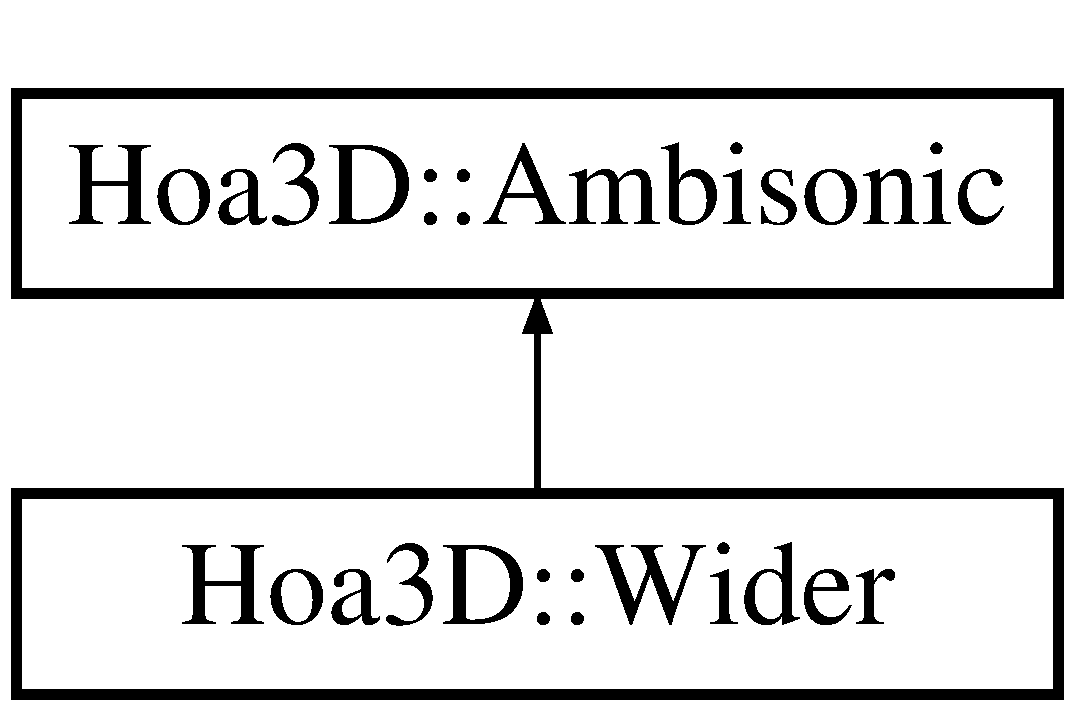
\includegraphics[height=2.000000cm]{class_hoa3_d_1_1_wider}
\end{center}
\end{figure}
\subsection*{Public Member Functions}
\begin{DoxyCompactItemize}
\item 
\hyperlink{class_hoa3_d_1_1_wider_a7f1f80e3329872d06f8e81f60f24e102}{Wider} (unsigned int order)
\begin{DoxyCompactList}\small\item\em The wider constructor. \end{DoxyCompactList}\item 
\hyperlink{class_hoa3_d_1_1_wider_a4a2770414c2753a9c92740f02641db38}{$\sim$\-Wider} ()
\begin{DoxyCompactList}\small\item\em The wider destructor. \end{DoxyCompactList}\item 
void \hyperlink{class_hoa3_d_1_1_wider_a5981d4dafbb0d2ce4ea20ec7cd1fb114}{set\-Widening\-Value} (const double value)
\begin{DoxyCompactList}\small\item\em This method set the widening value. \end{DoxyCompactList}\item 
void \hyperlink{class_hoa3_d_1_1_wider_a605d68c56ca7a541a9e91bd2aa9a9ea0}{process} (const float $\ast$inputs, float $\ast$outputs)
\begin{DoxyCompactList}\small\item\em This method performs the widening with single precision. \end{DoxyCompactList}\item 
void \hyperlink{class_hoa3_d_1_1_wider_a94fa445b540cbafeaafa05d4ed1a20bf}{process} (const double $\ast$inputs, double $\ast$outputs)
\begin{DoxyCompactList}\small\item\em This method performs the widening with double precision. \end{DoxyCompactList}\item 
\hyperlink{class_hoa3_d_1_1_wider_a7f1f80e3329872d06f8e81f60f24e102}{Wider} (unsigned int order)
\begin{DoxyCompactList}\small\item\em The wider constructor. \end{DoxyCompactList}\item 
\hyperlink{class_hoa3_d_1_1_wider_a4a2770414c2753a9c92740f02641db38}{$\sim$\-Wider} ()
\begin{DoxyCompactList}\small\item\em The wider destructor. \end{DoxyCompactList}\item 
void \hyperlink{class_hoa3_d_1_1_wider_a5981d4dafbb0d2ce4ea20ec7cd1fb114}{set\-Widening\-Value} (const double value)
\begin{DoxyCompactList}\small\item\em This method set the widening value. \end{DoxyCompactList}\item 
void \hyperlink{class_hoa3_d_1_1_wider_a605d68c56ca7a541a9e91bd2aa9a9ea0}{process} (const float $\ast$inputs, float $\ast$outputs)
\begin{DoxyCompactList}\small\item\em This method performs the widening with single precision. \end{DoxyCompactList}\item 
void \hyperlink{class_hoa3_d_1_1_wider_a94fa445b540cbafeaafa05d4ed1a20bf}{process} (const double $\ast$inputs, double $\ast$outputs)
\begin{DoxyCompactList}\small\item\em This method performs the widening with double precision. \end{DoxyCompactList}\end{DoxyCompactItemize}


\subsection{Detailed Description}
The ambisonic wider. 

The wider should be used to widen the sound propagation. 

Definition at line 17 of file Wider.\-h.



\subsection{Constructor \& Destructor Documentation}
\hypertarget{class_hoa3_d_1_1_wider_a7f1f80e3329872d06f8e81f60f24e102}{\index{Hoa3\-D\-::\-Wider@{Hoa3\-D\-::\-Wider}!Wider@{Wider}}
\index{Wider@{Wider}!Hoa3D::Wider@{Hoa3\-D\-::\-Wider}}
\subsubsection[{Wider}]{\setlength{\rightskip}{0pt plus 5cm}Hoa3\-D\-::\-Wider\-::\-Wider (
\begin{DoxyParamCaption}
\item[{unsigned int}]{order}
\end{DoxyParamCaption}
)}}\label{class_hoa3_d_1_1_wider_a7f1f80e3329872d06f8e81f60f24e102}


The wider constructor. 

The wider constructor allocates and initialize the member values to computes spherical harmonics weighted coefficients depending of a decomposition order. The order must be at least 1.


\begin{DoxyParams}{Parameters}
{\em order} & The order. \\
\hline
\end{DoxyParams}


Definition at line 11 of file Wider.\-cpp.

\hypertarget{class_hoa3_d_1_1_wider_a4a2770414c2753a9c92740f02641db38}{\index{Hoa3\-D\-::\-Wider@{Hoa3\-D\-::\-Wider}!$\sim$\-Wider@{$\sim$\-Wider}}
\index{$\sim$\-Wider@{$\sim$\-Wider}!Hoa3D::Wider@{Hoa3\-D\-::\-Wider}}
\subsubsection[{$\sim$\-Wider}]{\setlength{\rightskip}{0pt plus 5cm}Hoa3\-D\-::\-Wider\-::$\sim$\-Wider (
\begin{DoxyParamCaption}
{}
\end{DoxyParamCaption}
)}}\label{class_hoa3_d_1_1_wider_a4a2770414c2753a9c92740f02641db38}


The wider destructor. 

The wider destructor free the memory. 

Definition at line 65 of file Wider.\-cpp.

\hypertarget{class_hoa3_d_1_1_wider_a7f1f80e3329872d06f8e81f60f24e102}{\index{Hoa3\-D\-::\-Wider@{Hoa3\-D\-::\-Wider}!Wider@{Wider}}
\index{Wider@{Wider}!Hoa3D::Wider@{Hoa3\-D\-::\-Wider}}
\subsubsection[{Wider}]{\setlength{\rightskip}{0pt plus 5cm}Hoa3\-D\-::\-Wider\-::\-Wider (
\begin{DoxyParamCaption}
\item[{unsigned int}]{order}
\end{DoxyParamCaption}
)}}\label{class_hoa3_d_1_1_wider_a7f1f80e3329872d06f8e81f60f24e102}


The wider constructor. 

The wider constructor allocates and initialize the member values to computes spherical harmonics weighted coefficients depending of a decomposition order. The order must be at least 1.


\begin{DoxyParams}{Parameters}
{\em order} & The order. \\
\hline
\end{DoxyParams}
\hypertarget{class_hoa3_d_1_1_wider_a4a2770414c2753a9c92740f02641db38}{\index{Hoa3\-D\-::\-Wider@{Hoa3\-D\-::\-Wider}!$\sim$\-Wider@{$\sim$\-Wider}}
\index{$\sim$\-Wider@{$\sim$\-Wider}!Hoa3D::Wider@{Hoa3\-D\-::\-Wider}}
\subsubsection[{$\sim$\-Wider}]{\setlength{\rightskip}{0pt plus 5cm}Hoa3\-D\-::\-Wider\-::$\sim$\-Wider (
\begin{DoxyParamCaption}
{}
\end{DoxyParamCaption}
)}}\label{class_hoa3_d_1_1_wider_a4a2770414c2753a9c92740f02641db38}


The wider destructor. 

The wider destructor free the memory. 

\subsection{Member Function Documentation}
\hypertarget{class_hoa3_d_1_1_wider_a605d68c56ca7a541a9e91bd2aa9a9ea0}{\index{Hoa3\-D\-::\-Wider@{Hoa3\-D\-::\-Wider}!process@{process}}
\index{process@{process}!Hoa3D::Wider@{Hoa3\-D\-::\-Wider}}
\subsubsection[{process}]{\setlength{\rightskip}{0pt plus 5cm}void Hoa3\-D\-::\-Wider\-::process (
\begin{DoxyParamCaption}
\item[{const float $\ast$}]{inputs, }
\item[{float $\ast$}]{outputs}
\end{DoxyParamCaption}
)}}\label{class_hoa3_d_1_1_wider_a605d68c56ca7a541a9e91bd2aa9a9ea0}


This method performs the widening with single precision. 

You should use this method for in-\/place or not-\/in-\/place processing and performs the widening sample by sample. The inputs array and outputs array contains the spherical harmonics samples and the minimum size must be the number of harmonics.


\begin{DoxyParams}{Parameters}
{\em inputs} & The input array. \\
\hline
{\em outputs} & The output array. \\
\hline
\end{DoxyParams}


Definition at line 53 of file Wider.\-cpp.

\hypertarget{class_hoa3_d_1_1_wider_a605d68c56ca7a541a9e91bd2aa9a9ea0}{\index{Hoa3\-D\-::\-Wider@{Hoa3\-D\-::\-Wider}!process@{process}}
\index{process@{process}!Hoa3D::Wider@{Hoa3\-D\-::\-Wider}}
\subsubsection[{process}]{\setlength{\rightskip}{0pt plus 5cm}void Hoa3\-D\-::\-Wider\-::process (
\begin{DoxyParamCaption}
\item[{const float $\ast$}]{inputs, }
\item[{float $\ast$}]{outputs}
\end{DoxyParamCaption}
)}}\label{class_hoa3_d_1_1_wider_a605d68c56ca7a541a9e91bd2aa9a9ea0}


This method performs the widening with single precision. 

You should use this method for in-\/place or not-\/in-\/place processing and performs the widening sample by sample. The inputs array and outputs array contains the spherical harmonics samples and the minimum size must be the number of harmonics.


\begin{DoxyParams}{Parameters}
{\em inputs} & The input array. \\
\hline
{\em outputs} & The output array. \\
\hline
\end{DoxyParams}
\hypertarget{class_hoa3_d_1_1_wider_a94fa445b540cbafeaafa05d4ed1a20bf}{\index{Hoa3\-D\-::\-Wider@{Hoa3\-D\-::\-Wider}!process@{process}}
\index{process@{process}!Hoa3D::Wider@{Hoa3\-D\-::\-Wider}}
\subsubsection[{process}]{\setlength{\rightskip}{0pt plus 5cm}void Hoa3\-D\-::\-Wider\-::process (
\begin{DoxyParamCaption}
\item[{const double $\ast$}]{inputs, }
\item[{double $\ast$}]{outputs}
\end{DoxyParamCaption}
)}}\label{class_hoa3_d_1_1_wider_a94fa445b540cbafeaafa05d4ed1a20bf}


This method performs the widening with double precision. 

You should use this method for in-\/place or not-\/in-\/place processing and performs the widening sample by sample. The inputs array and outputs array contains the spherical harmonics samples and the minimum size must be the number of harmonics.


\begin{DoxyParams}{Parameters}
{\em inputs} & The input array. \\
\hline
{\em outputs} & The output array. \\
\hline
\end{DoxyParams}
\hypertarget{class_hoa3_d_1_1_wider_a94fa445b540cbafeaafa05d4ed1a20bf}{\index{Hoa3\-D\-::\-Wider@{Hoa3\-D\-::\-Wider}!process@{process}}
\index{process@{process}!Hoa3D::Wider@{Hoa3\-D\-::\-Wider}}
\subsubsection[{process}]{\setlength{\rightskip}{0pt plus 5cm}void Hoa3\-D\-::\-Wider\-::process (
\begin{DoxyParamCaption}
\item[{const double $\ast$}]{inputs, }
\item[{double $\ast$}]{outputs}
\end{DoxyParamCaption}
)}}\label{class_hoa3_d_1_1_wider_a94fa445b540cbafeaafa05d4ed1a20bf}


This method performs the widening with double precision. 

You should use this method for in-\/place or not-\/in-\/place processing and performs the widening sample by sample. The inputs array and outputs array contains the spherical harmonics samples and the minimum size must be the number of harmonics.


\begin{DoxyParams}{Parameters}
{\em inputs} & The input array. \\
\hline
{\em outputs} & The output array. \\
\hline
\end{DoxyParams}


Definition at line 59 of file Wider.\-cpp.

\hypertarget{class_hoa3_d_1_1_wider_a5981d4dafbb0d2ce4ea20ec7cd1fb114}{\index{Hoa3\-D\-::\-Wider@{Hoa3\-D\-::\-Wider}!set\-Widening\-Value@{set\-Widening\-Value}}
\index{set\-Widening\-Value@{set\-Widening\-Value}!Hoa3D::Wider@{Hoa3\-D\-::\-Wider}}
\subsubsection[{set\-Widening\-Value}]{\setlength{\rightskip}{0pt plus 5cm}void Hoa3\-D\-::\-Wider\-::set\-Widening\-Value (
\begin{DoxyParamCaption}
\item[{const double}]{value}
\end{DoxyParamCaption}
)}}\label{class_hoa3_d_1_1_wider_a5981d4dafbb0d2ce4ea20ec7cd1fb114}


This method set the widening value. 

The widening value is clipped between 0 and 1. At 1, the sound field has no changes. At 0, all the sound field is omni directionnal.


\begin{DoxyParams}{Parameters}
{\em value} & The widening value. \\
\hline
\end{DoxyParams}
\hypertarget{class_hoa3_d_1_1_wider_a5981d4dafbb0d2ce4ea20ec7cd1fb114}{\index{Hoa3\-D\-::\-Wider@{Hoa3\-D\-::\-Wider}!set\-Widening\-Value@{set\-Widening\-Value}}
\index{set\-Widening\-Value@{set\-Widening\-Value}!Hoa3D::Wider@{Hoa3\-D\-::\-Wider}}
\subsubsection[{set\-Widening\-Value}]{\setlength{\rightskip}{0pt plus 5cm}void Hoa3\-D\-::\-Wider\-::set\-Widening\-Value (
\begin{DoxyParamCaption}
\item[{const double}]{value}
\end{DoxyParamCaption}
)}}\label{class_hoa3_d_1_1_wider_a5981d4dafbb0d2ce4ea20ec7cd1fb114}


This method set the widening value. 

The widening value is clipped between 0 and 1. At 1, the sound field has no changes. At 0, all the sound field is omni directionnal.


\begin{DoxyParams}{Parameters}
{\em value} & The widening value. \\
\hline
\end{DoxyParams}


Definition at line 48 of file Wider.\-cpp.



The documentation for this class was generated from the following files\-:\begin{DoxyCompactItemize}
\item 
/\-Users/elioton/\-Documents/programmation/\-C\-I\-C\-M/source\-Tree/\-Hoa\-Library/\-Sources/\-Hoa3\-D/Wider.\-h\item 
/\-Users/elioton/\-Documents/programmation/\-C\-I\-C\-M/source\-Tree/\-Hoa\-Library/\-Sources/hoa\-Wider/Hoa3\-D\-Wider.\-h\item 
/\-Users/elioton/\-Documents/programmation/\-C\-I\-C\-M/source\-Tree/\-Hoa\-Library/\-Sources/\-Hoa3\-D/Wider.\-cpp\item 
/\-Users/elioton/\-Documents/programmation/\-C\-I\-C\-M/source\-Tree/\-Hoa\-Library/\-Sources/hoa\-Wider/Hoa3\-D\-Wider.\-cpp\end{DoxyCompactItemize}

%--- End generated contents ---

% Index
\newpage
\phantomsection
\addcontentsline{toc}{part}{Index}
\printindex

\end{document}
